%!TEX TS-program = xelatex
%!TEX encoding = UTF-8 Unicode

\documentclass[a4paper, 11pt, twoside]{StyleThese}
\usepackage{psl-cover}
\DeclareGraphicsExtensions{.pdf, .jpeg, .png}
%!TEX root = ./main.tex

\usepackage{acronym}

\newacro{DNA}{Deoxyribonucleic Acid}
\newacro{RNA}{Ribonucleic Acid}
\newacro{mRNA}{Messenger RNA}
\newacro{rRNA}{Ribosomal RNA}
\newacro{tRNA}{Transfer RNA}
\newacro{CBIO}{Center for Computational Biology}
\newacro{Inserm}{French National Institute of Health and Medical Research}
\newacro{IGMM}{Institute of Molecular Genetics of Montpellier}
\newacro{FISH}{Fluorescence In Situ Hybridization}
\newacro{smFISH}{single molecule FISH}
\newacro{smiFISH}{single molecule inexpensive FISH}
\newacro{SeqFISH}{Sequential FISH}
\newacro{MERFISH}{Multiplexed Error-Robust FISH}
\newacro{PCA}{Principal Component Analysis}
\newacro{LoG}{Laplacian of Gaussian}
\newacro{DoG}{Difference of Gaussians}
\newacro{GAN}{Generative Adversarial Network}
\newacro{PSF}{Point-Spread-Function}
\newacro{GFP}{Green Fluorescent Protein}
\newacro{SNR}{Signal-to-Noise Ratio}
\newacro{FoV}{Field of View}
\newacro{GUI}{Graphical User Interface}
\newacro{CASO}{Context Aggregation for Small Objects}
\newacro{MTOC}{Main Microtubule Organizing Center}
%!TEX root = ./main.tex

\usepackage{lipsum}
\usepackage{amsmath, amssymb, amsthm, amsfonts, dsfont, mathabx}
\usepackage{cancel}
\usepackage{cite}
\usepackage[english]{babel}
\usepackage[utf8x]{inputenc}
\usepackage[T1]{fontenc}
\usepackage{lmodern}
\usepackage[left=3.5cm, right=3.0cm, top=2.2cm, bottom=2.2cm, includefoot, includehead, headheight=13.6pt]{geometry}
\renewcommand{\baselinestretch}{1.05}

% Table of contents for each chapter
\usepackage[nottoc, notlof, notlot]{tocbibind}
\usepackage[english]{minitoc}
\setcounter{minitocdepth}{2}
\mtcindent=15pt  % use \minitoc where to put a table of contents
\usepackage{aecompl}

% Glossary / list of abbreviations
\usepackage{multicol}
\usepackage[intoc]{nomencl}
\renewcommand{\nomname}{Glossary of terms, Abbreviations, \\ Acronyms and Symbols}
\makenomenclature
\makenomenclature
\setlength{\nomitemsep}{-\parsep}
\setlength{\nomitemsep}{0.05pt}

% python code
\usepackage{listings}
\usepackage{xcolor}
\definecolor{red}{rgb}{0.698, 0.1333, 0.1333}
\definecolor{green}{rgb}{0.1333, 0.5451, 0.1333}
\definecolor{blue}{rgb}{0.275, 0.51, 0.706}
\definecolor{gray}{rgb}{0.45, 0.45, 0.45}
\definecolor{lightgray}{rgb}{0.97, 0.97, 0.97}
\definecolor{black}{rgb}{0, 0, 0}
\lstdefinestyle{mystyle}{
    backgroundcolor=\color{lightgray},
    commentstyle=\color{gray},
    keywordstyle=\color{green},
    numberstyle=\color{black},
    stringstyle=\color{red},
    basicstyle=\ttfamily\footnotesize,
	rulecolor=\color{black},
	frame=single,
    breakatwhitespace=false,
    breaklines=false,
    captionpos=b,
    keepspaces=true,
    numbers=none,
    numbersep=0pt,
    showspaces=false,
    showstringspaces=false,
    showtabs=false,
    tabsize=4
}
\lstset{style=mystyle}

\usepackage{wrapfig}

%----------------------------------------------

\setcounter{secnumdepth}{2}
\setcounter{tocdepth}{2}

\usepackage{rotating}
\usepackage{fancyhdr}

% Fancy Header Style Options
\pagestyle{fancy}
\fancyfoot{}
\fancyhead[LE, RO]{\bfseries\thepage}

% Pages and right on odd pages
\fancyhead[RE]{\bfseries\nouppercase{\leftmark}}
\fancyhead[LO]{\bfseries\nouppercase{\rightmark}}

\let\headruleORIG\headrule
\renewcommand{\headrule}{\color{black} \headruleORIG}
\renewcommand{\headrulewidth}{1.0pt}
\usepackage{colortbl}
\arrayrulecolor{black}

\fancypagestyle{plain}{
  \fancyhead{}
  \fancyfoot{}
  \fancyhf{}
  \renewcommand{\headrulewidth}{0pt}
}

%----------------------------------------------

% Clear Header Style on the Last Empty Odd pages
\makeatletter

\def\cleardoublepage{\clearpage\if@twoside \ifodd\c@page\else%
  \hbox{}%
  \thispagestyle{empty}%              % Empty header styles
  \newpage%
  \if@twocolumn\hbox{}\newpage\fi\fi\fi}

\makeatother
 
%%%%%%%%%%%%%%%%%%%%%%%%%%%%%%%%%%%%%%%%%%%%%%%%%%%%%%%%%%%%%%%%%%%%%%%%%%%%%%% 
% Prints your review date and 'Draft Version' (From Josullvn, CS, CMU)
\newcommand{\reviewtimetoday}[2]{\special{!userdict begin
    /bop-hook{gsave 20 710 translate 45 rotate 0.8 setgray
      /Times-Roman findfont 12 scalefont setfont 0 0   moveto (#1) show
      0 -12 moveto (#2) show grestore}def end}}
% You can turn on or off this option.
\reviewtimetoday{\today}{Draft Version}
%%%%%%%%%%%%%%%%%%%%%%%%%%%%%%%%%%%%%%%%%%%%%%%%%%%%%%%%%%%%%%%%%%%%%%%%%%%%%%% 

\newenvironment{maxime}[1]
{
\vspace*{0cm}
\hfill
\begin{minipage}{0.5\textwidth}%
%\rule[0.5ex]{\textwidth}{0.1mm}\\%
\hrulefill $\:$ {\bf #1}\\
%\vspace*{-0.25cm}
\it 
}%
{%

\hrulefill
\vspace*{0.5cm}%
\end{minipage}
}

\let\minitocORIG\minitoc
\renewcommand{\minitoc}{\minitocORIG \vspace{1.5em}}

\usepackage{multirow}
\usepackage{diagbox}

\newenvironment{bulletList}%
{ \begin{list}%
	{$\bullet$}%
	{\setlength{\labelwidth}{25pt}%
	 \setlength{\leftmargin}{30pt}%
	 \setlength{\itemsep}{\parsep}}}%
{ \end{list} }

\newtheorem{definition}{Definition}
\renewcommand{\epsilon}{\varepsilon}

% centered page environment

\newenvironment{vcenterpage}
{\newpage\vspace*{\fill}\thispagestyle{empty}\renewcommand{\headrulewidth}{0pt}}
{\vspace*{\fill}}

% Change this to change the informations included in the pdf file

\usepackage[palatino]{quotchap}
\usepackage{tikz}
\usepackage{adjustbox} % scaling pictures
\usepackage{afterpage} % allows for the rotation

\usepackage{pifont}
\usepackage{subcaption}

% \usepackage{fontspec}

\usepackage{setspace}

% %%\usepackage[pdftex]{graphicx}
%\usepackage{subfig} %for subfloat images
\usepackage{stmaryrd}

\usepackage{algorithmic}
\usepackage{algorithm}
\usepackage[titletoc]{appendix}

% \usepackage{floatpag} % so that with sideway figures i can remove the page number
\newcommand{\acknowledgments}{
  \chapter*{Acknowledgments}
  \noindent

      %!TEX root = ./main.tex

% acknowledgments section
\chapter*{Aknowledgment} \addcontentsline{toc}{chapter}{Aknowledgment} \adjustmtc
\markboth{Aknowledgement}{Aknowledgement}

Au moment d'écrire les derniers mots de ce manuscrit, l'occasion se présente d'apprécier le chemin parcouru.
Si l'exercice d'une thèse reste une tâche solitaire, sa réussite n'en demeure pas moins liée aux rencontres que l'on fait.
J'aimerais remercier ici toutes les personnes qui ont pu compter ces dernières années, par leur présence et leur soutien.\\

Mes premiers remerciements vont bien évidemment à Thomas et Florian.
Un très grand merci pour m'avoir fait confiance et avoir accepté d'encadrer ma thèse.
Merci d'avoir fait le chercheur que je suis aujourd'hui, merci pour votre bonne humeur, votre optimisme et votre écoute.
Je trouve que nous avons formé une belle équipe et nos (parfois trop longues) réunions vont me manquer !
J'aimerais également exprimer ma gratitude envers Edouard Bertrand et son équipe, notamment Adham, Xavier et Emeline.
Notre collaboration n'aurait pas été aussi réussie sans votre accueil enthousiaste à Montpellier, ni votre expertise.
Enfin, c'est aux membres de mon jury que je souhaite adresser de sincères remerciements.
Etienne Decencière, Carolina Wählby, Marcelo Nollmann et Perrine Paul-Gilloteaux, merci de me faire l'honneur de lire et de juger mes travaux de thèse.\\

Ces dernières années si particulières ont pu mettre en évidence à quel point la vie d'un laboratoire pouvait être importante pour notre recherche.
Merci à la grande famille du CBIO pour votre enthousiasme, les discussions, les pauses cafés, et tout simplement pour partager les bons et les mauvais moments d'une thèse.

Mes pensées vont tout particulièrement à Chloé, Florian et Véronique pour leur leadership et leur bienveillance au quotidien.
J'aimerais mentionner Asma, avec qui j'ai commencé cette aventure au CBIO, ainsi que la vieille garde composée de Benoit, Judith, Lotfi, Romain, Joseph et surtout Peter, pour votre accueil chaleureux à mon arrivée dans l'équipe.
Merci à Thomas B. et Mélanie, pour cette improbable conférence en Terre Sainte, à Thomas D. qui, plus que tout autre dans l'équipe, a pu partager mes joies et mes peines du FISH et à Maxence, dont je garde un très bon souvenir de notre \emph{paper reading group} du vendredi.
Pouvoir encadrer ton stage a été une très belle expérience, malgré des conditions qui n'ont pas été toujours évidentes.
Je remercie également Gwenaëlle, Julie, Aurélie et Philippe pour m'avoir fait découvrir vos talents de danseur, Matthieu N. (avec qui j'ai l'impression de partager 950 amis et connaissances) pour faire Movember sur 12 mois de l'année, Maguette pour tes précieux conseils en cuisine, Gwenn pour nos débats politiques et discussions hautement philosophiques, Tristan toujours prêt à "jouer" avec le nouveau modèle à la mode, Elise, dont je regrette de n'avoir pas pu assister à ta superbe soutenance, même si j'avais une très bonne raison ce jour là, Marvin, \emph{a hell of a researcher}, Adeline pour ton énergie et tes \emph{good vibes} au quotidien, Daniel R. pour ta motivation et ton assiduité à participer aux book clubs et autres séminaires, Vincent pour ta curiosité, ton enthousiasme et ta patience lorsqu'il s'agit de nous (ré)apprendre la géométrie et Anne qui a décidé de mener de front une carrière de chercheuse et de médecin (parce qu'une seule des deux aurait été trop facile).
La vie d'un laboratoire ne se limite pas à la recherche et c'est pourquoi je remercie grandement Caroline, Katy et Pamela pour leur aide quotidienne aux Mines ou à l'Institut Curie, et surtout pour m'avoir supporté avec ma phobie administrative.\\

Ma dernière salve de remerciements est réservée aux personnes extérieures au CBIO qui m'ont accompagnée, formée et soutenue.

Merci Mr. Peltan et Mr. Brochier, je vous dois beaucoup.
Quand je suis venu vous voir il y a quelques années avec l'idée un peu loufoque de passer un concours en candidat libre, à ma grande surprise, vous avez accepté de m'aider.
Sans vous, mon parcours aurait été bien différent.
Irène, Gaël et Catherine, merci de m'avoir mentoré.
Tous les trois docteurs, tous les trois extrêmement compétents et bienveillants, c'est avec vos conseils et votre exemple en tête que je me suis lancé dans cette thèse.

Un grand merci enfin à mes amis et à ma famille.
Merci à Thibaut toujours présent malgré l'éloignement et le temps qui passe et que je ne saurais classer parmi les amis ou la famille.
Merci à Guillaume, Lucas, Théo, Florian V., Mathieu M., Hugo, Mathieu G., Adrien, Claire, Victor, Florian L. et Alexandre pour tous les weekends, les soirées (oubliées ou à oublier), les brunchs, les vacances et autres souvenirs partagés avec vous.
Merci à la famille du Caire, Elisa et Gauthier, pour avoir rendu la vie parisienne si agréable.
Merci à mes grand-parents.
Néné, comme tu me l'as si bien dit, cette thèse c'est aussi un peu grâce à toi.
Papa et Maman, merci pour votre soutien et votre amour.
Merci Juna, merci Poppy, pour me donner la meilleure des raisons pour descendre les weekends à Marseille.

Finalement, ces remerciements ne seraient pas complets sans un dernier mot pour Mary, celle dont le soutien a été si important pour moi ces dernières années.
L'aventure n'aurait pas été aussi belle sans toi.
Du fond du coeur, merci.

  \vspace*{\fill} \newpage
  \setcounter{page}{1}
  \pagenumbering{arabic}
}

\usepackage[mathscr]{eucal}
\usepackage{textcomp}

\newenvironment{theabstract}[1]%
{\markboth{#1}{#1}%
{\large\noindent\rule{1ex}{1ex}\hspace{\stretch{1}}%
{\textbf{\textit{#1}}}%
\hspace{\stretch{1}}\rule{1ex}{1ex}}
\addcontentsline{toc}{chapter}{#1} \adjustmtc
\vskip 0.2in
\begin{large}}%
{\end{large}}

\newcolumntype{R}[2]{%
    >{\adjustbox{angle=#1,lap=\width-(#2)}\bgroup}%
    l%
    <{\egroup}%
}
\newcommand*\rot{\multicolumn{1}{R{70}{1em}}}  % no optional argument here, please!

%----------------------------------------------

% Links in pdf
\usepackage{xcolor}
\definecolor{linkcol}{rgb}{0,0,0.4} 
\definecolor{citecol}{rgb}{0.5,0,0}
\usepackage{hyperref}
\hypersetup
{
pdftitle="manuscript",
pdfauthor="Arthur Imbert", %auteur du document
pdfsubject="Bioinformatic", %sujet du document
pdfmenubar=true, %barre de menu visible
pdfhighlight=/O, %effect of clicking on a link
colorlinks=true, %couleurs sur les liens hypertextes
pdfpagemode=UseNone, %aucun mode de page
pdfpagelayout=SinglePage, %ouverture en simple page
pdffitwindow=true, %pages ouvertes entierement dans toute la fenetre
linkcolor=linkcol, %couleur des liens hypertextes internes
citecolor=citecol, %couleur des liens pour les citations
urlcolor=linkcol %couleur des liens pour les url
}

%----------------------------------------------

\begin{document}
\dominitoc

% frontmatter
%!TEX root = ./main.tex

% Some details about the dissertation.
\title{Next generation tools for image based transcriptomics}

\author{Arthur Imbert}

\doctoralschool{Ingénierie des Systèmes, Matériaux, Mécaniques, Énergétique}{621}
\specialty{Bio-informatique}
\date{}

\jurymember{1}{Prenom1 NOM1}{Titre \\ Ecole, Pays}{President}

\jurymember{2}{Prenom2 NOM2}{Titre \\ Ecole, Pays}{Rapporteur}

\jurymember{3}{Prenom3 NOM3}{Titre \\ Ecole, Pays}{Rapporteur}

\jurymember{4}{Prenom4 NOM4}{Titre \\ Ecole, Pays}{Examinateur}

\jurymember{5}{Prenom5 NOM5}{Titre \\ Ecole, Pays}{Examinateur}

\jurymember{6}{Florian Mueller}{Titre \\ Institut Pasteur, France}{Directeur de thèse}

\jurymember{7}{Thomas Walter}{Titre \\ Mines ParisTech, France}{Directeur de thèse}

%\maketitle{}
\frontmatter
%%!TEX root = ./main.tex

\frkeywords{French keywords}
\frabstract{ 
French abstract
}
%%!TEX root = ./main.tex

\enkeywords{Key words}
\enabstract{ 
English abstract
}

%%!TEX root = ./main.tex

% acknowledgments section
\chapter*{Aknowledgment} \addcontentsline{toc}{chapter}{Aknowledgment} \adjustmtc
\markboth{Aknowledgement}{Aknowledgement}

Au moment d'écrire les derniers mots de ce manuscrit, l'occasion se présente d'apprécier le chemin parcouru.
Si l'exercice d'une thèse reste une tâche solitaire, sa réussite n'en demeure pas moins liée aux rencontres que l'on fait.
J'aimerais remercier ici toutes les personnes qui ont pu compter ces dernières années, par leur présence et leur soutien.\\

Mes premiers remerciements vont bien évidemment à Thomas et Florian.
Un très grand merci pour m'avoir fait confiance et avoir accepté d'encadrer ma thèse.
Merci d'avoir fait le chercheur que je suis aujourd'hui, merci pour votre bonne humeur, votre optimisme et votre écoute.
Je trouve que nous avons formé une belle équipe et nos (parfois trop longues) réunions vont me manquer !
J'aimerais également exprimer ma gratitude envers Edouard Bertrand et son équipe, notamment Adham, Xavier et Emeline.
Notre collaboration n'aurait pas été aussi réussie sans votre accueil enthousiaste à Montpellier, ni votre expertise.
Enfin, c'est aux membres de mon jury que je souhaite adresser de sincères remerciements.
Etienne Decencière, Carolina Wählby, Marcelo Nollmann et Perrine Paul-Gilloteaux, merci de me faire l'honneur de lire et de juger mes travaux de thèse.\\

Ces dernières années si particulières ont pu mettre en évidence à quel point la vie d'un laboratoire pouvait être importante pour notre recherche.
Merci à la grande famille du CBIO pour votre enthousiasme, les discussions, les pauses cafés, et tout simplement pour partager les bons et les mauvais moments d'une thèse.

Mes pensées vont tout particulièrement à Chloé, Florian et Véronique pour leur leadership et leur bienveillance au quotidien.
J'aimerais mentionner Asma, avec qui j'ai commencé cette aventure au CBIO, ainsi que la vieille garde composée de Benoit, Judith, Lotfi, Romain, Joseph et surtout Peter, pour votre accueil chaleureux à mon arrivée dans l'équipe.
Merci à Thomas B. et Mélanie, pour cette improbable conférence en Terre Sainte, à Thomas D. qui, plus que tout autre dans l'équipe, a pu partager mes joies et mes peines du FISH et à Maxence, dont je garde un très bon souvenir de notre \emph{paper reading group} du vendredi.
Pouvoir encadrer ton stage a été une très belle expérience, malgré des conditions qui n'ont pas été toujours évidentes.
Je remercie également Gwenaëlle, Julie, Aurélie et Philippe pour m'avoir fait découvrir vos talents de danseur, Matthieu N. (avec qui j'ai l'impression de partager 950 amis et connaissances) pour faire Movember sur 12 mois de l'année, Maguette pour tes précieux conseils en cuisine, Gwenn pour nos débats politiques et discussions hautement philosophiques, Tristan toujours prêt à "jouer" avec le nouveau modèle à la mode, Elise, dont je regrette de n'avoir pas pu assister à ta superbe soutenance, même si j'avais une très bonne raison ce jour là, Marvin, \emph{a hell of a researcher}, Adeline pour ton énergie et tes \emph{good vibes} au quotidien, Daniel R. pour ta motivation et ton assiduité à participer aux book clubs et autres séminaires, Vincent pour ta curiosité, ton enthousiasme et ta patience lorsqu'il s'agit de nous (ré)apprendre la géométrie et Anne qui a décidé de mener de front une carrière de chercheuse et de médecin (parce qu'une seule des deux aurait été trop facile).
La vie d'un laboratoire ne se limite pas à la recherche et c'est pourquoi je remercie grandement Caroline, Katy et Pamela pour leur aide quotidienne aux Mines ou à l'Institut Curie, et surtout pour m'avoir supporté avec ma phobie administrative.\\

Ma dernière salve de remerciements est réservée aux personnes extérieures au CBIO qui m'ont accompagnée, formée et soutenue.

Merci Mr. Peltan et Mr. Brochier, je vous dois beaucoup.
Quand je suis venu vous voir il y a quelques années avec l'idée un peu loufoque de passer un concours en candidat libre, à ma grande surprise, vous avez accepté de m'aider.
Sans vous, mon parcours aurait été bien différent.
Irène, Gaël et Catherine, merci de m'avoir mentoré.
Tous les trois docteurs, tous les trois extrêmement compétents et bienveillants, c'est avec vos conseils et votre exemple en tête que je me suis lancé dans cette thèse.

Un grand merci enfin à mes amis et à ma famille.
Merci à Thibaut toujours présent malgré l'éloignement et le temps qui passe et que je ne saurais classer parmi les amis ou la famille.
Merci à Guillaume, Lucas, Théo, Florian V., Mathieu M., Hugo, Mathieu G., Adrien, Claire, Victor, Florian L. et Alexandre pour tous les weekends, les soirées (oubliées ou à oublier), les brunchs, les vacances et autres souvenirs partagés avec vous.
Merci à la famille du Caire, Elisa et Gauthier, pour avoir rendu la vie parisienne si agréable.
Merci à mes grand-parents.
Néné, comme tu me l'as si bien dit, cette thèse c'est aussi un peu grâce à toi.
Papa et Maman, merci pour votre soutien et votre amour.
Merci Juna, merci Poppy, pour me donner la meilleure des raisons pour descendre les weekends à Marseille.

Finalement, ces remerciements ne seraient pas complets sans un dernier mot pour Mary, celle dont le soutien a été si important pour moi ces dernières années.
L'aventure n'aurait pas été aussi belle sans toi.
Du fond du coeur, merci.

\cleardoublepage
\tableofcontents

\cleardoublepage
\listoffigures \addcontentsline{toc}{chapter}{\listfigurename} \adjustmtc
\listoftables \addcontentsline{toc}{chapter}{\listtablename} \adjustmtc

% mainmatter
\mainmatter

\setcounter{chapter}{0}  % start chapter numbering at 0

%\part{Introduction}
%%!TEX root = ../main.tex

\graphicspath{{./figures/introduction/}}

\chapter{FISH-based transcriptomics}
\label{ch:introduction}

\minitoc
\newpage

In this introduction, I will present the gene expression process in order to describe the biological context where \ac{RNA} localization happens.
Then, I will present the experimental protocols that allows us to visualize and analyse \ac{RNA} molecules as well as the machine learning tools I applied.
I will finish this introduction with an overview of my thesis goals, a list of the contributions I made and a summary of this manuscript to guide the reader.

\section{Gene expression process}
\label{sec:gene_expression}

Cells are the basic unit of all living organisms.
Yet, a diversity of cell-type exists, performing different actions.
Some of those are common among all cells (cell division for example), but others can be very specific.
Most of the time, different cell-types perform diverse actions through a different set of functional molecules.
In order to implement these different cellular processes and to fulfill the variety of diverse functions, a cell gets its instructions from the \ac{DNA}.
The latter contains all the cell's genetic information and it is common for all cells of the same organism.
A \ac{DNA} strand presents a succession of genes, defined as long sequences of nucleotides.
They are organics molecules composed of a five-carbon sugar, a phosphate group and one of the four nucleobases: Adenine, Cytosine, Guanine and Thymine.
Together, these nucleobases form a genetic alphabet of 4 letters (A, C, G and  T).
Each gene encodes the blueprint of a functional molecule with a specific sequence of nucleobases.

Gene expression is the process by which genetic information is transformed into functional products.
\ac{RNA} molecules, or transcripts, are essential for this process.
They are either the functional gene products themselves or they serve as an intermediate molecule prior to the production of other functional products, namely the proteins.
A change in gene expression gives cells enough flexibility to adapt and react to different external stimuli.
It also drives cells differentiation, allows them to run their basic functions, modulate their activities and therefore appears to be one of the most fundamental processes of life.
On the contrary, its deregulation can lead to various diseases.
This explains the interest of the scientific community to study and decode gene expression processes.

In the living world, cells can be divided in two categories: prokaryotic cells and eukaryotic cells.
The prokaryotic cells, which do not have a nucleus and typically form a unicellular organism, and the eukaryotic cells, with a well-organized nucleus.
An eukaryote (a living organism with eukaryotic cells) is usually composed of cells with a higher level of compartmentalization through membrane-bound organelles.
The nucleus is obviously the most important of these organelles, with the \ac{DNA} inside.
The rest of the organelles are located in the cytoplasm, such as the mitochondria, the lysosomes, or the Golgi apparatus (see Figure~\ref{fig:eukaryotic_cell}).

For an eukaryote cell, the expression of a gene includes two main steps: the transcription of a \ac{DNA} sequence into a \ac{RNA} (in the nucleus) and the translation of a \ac{RNA} into a protein.
Between these two major steps, there is a phase of maturation for the transcript, before a potential exports outside the nucleus and a transport somewhere in the cytoplasm.
A cell can regulate either the transcription or the translation step to control the production of its functional molecules and thereby the biological process to which the proteins or \ac{RNA} contribute\footnote{For a complete and general introduction about cellular biology, an interested reader could see~\cite{alberts_molecular_2017}.}.

\begin{figure}[]
    \centering
    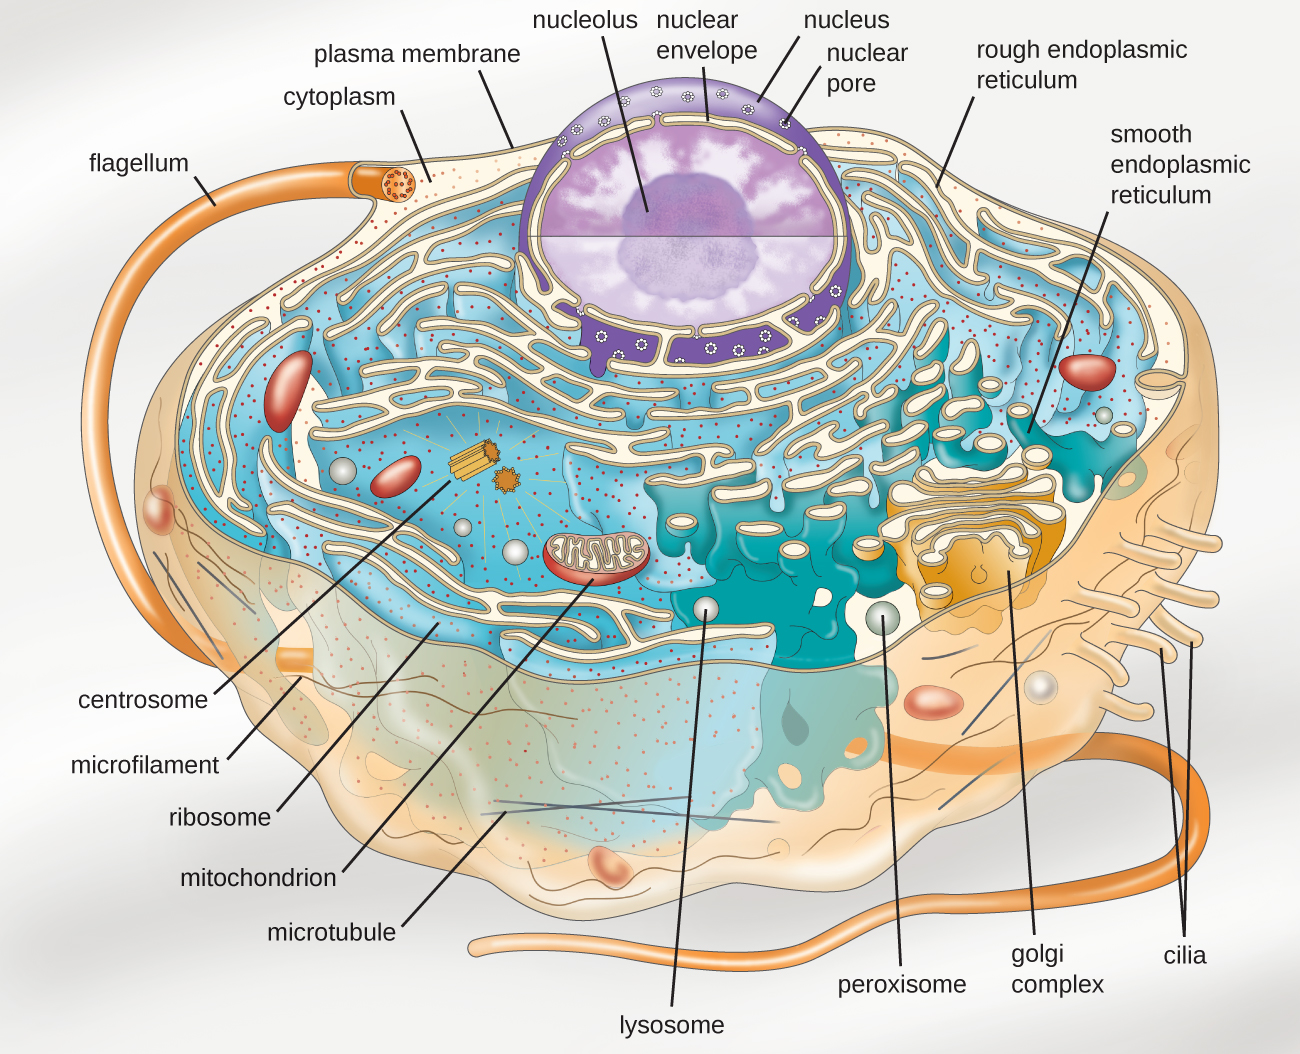
\includegraphics[width=0.8\textwidth]{figures/introduction/cell_eukaryotic.jpg}
    \caption[Illustration of an eukaryotic cell]{Illustration of an eukaryotic cell, from~\cite{parker2017microbiology}}
    \label{fig:eukaryotic_cell}
\end{figure}

\subsection{Transcription}
\label{subsec:intro_transcription}

\subsubsection{The primary transcripts}

This step consists in copying a gene (a sequence of nucleotides along the \ac{DNA} strands) into another biomolecules composed of nucleotides: a \ac{RNA}.
While the \ac{DNA} is stuck within the nucleus, the \ac{RNA} can convey the blueprint of the future protein outside.
In many cases, \ac{RNA} can be non-coding (they do not lead to the synthesis of a protein) and fulfill a variety of functions itself, for instance the regulation of gene expression.
In a \ac{RNA}, the nucleotide Uracil (U) replaces the Thymine (T) and a ribose sugar serves as backbone instead of a desoxyribose sugar.
If both \ac{DNA} and \ac{RNA} contain genetic information, \ac{RNA} is a shorter single-stranded molecule, compared to the double-stranded \ac{DNA}, and, therefore, is less stable.
However, they both have two distinctive untranslated regions at their ends: 5'UTR and 3'UTR (corresponding to the number of carbon atoms in their sugar backbone extremities).\\

\noindent
Transcription proceeds as follows:
\begin{enumerate}
	\setlength\itemsep{0.1em}
	\item Proteins that serve as transcription factors bind to a specific sequence of \ac{DNA} (the promoter sequence) and recruit an enzyme (the \ac{RNA} polymerase) to initiate the transcription.
	\item The \ac{RNA} polymerase breaks the hydrogen bounds between the two \ac{DNA} strands to separate them.
	\item The \ac{RNA} polymerase moves along one \ac{DNA} strand, from 3' to 5' extremity, synthesizing a complementary nucleotides sequence on the way.
	\item The \ac{RNA} polymerase disengages from the strand when it meets a specific sequence of \ac{DNA} (the terminator sequence) and the newly synthesized nucleotides sequence (the primary transcribed \ac{RNA}) is released.
\end{enumerate}

\noindent
At this point, different sorts of \ac{RNA} are transcribed, depending of \ac{RNA} polymerase recruited:
\begin{itemize}
	\setlength\itemsep{0.1em}
	\item \ac{mRNA}, composed of coding (exon) and non-coding (intron) nucleotides, which conveys the blueprint of a future protein.
	\item \ac{rRNA} which, associated with ribosomal proteins, forms ribosomes, a macromolecular machine used by the cell to synthesize proteins.
	\item \ac{tRNA}, the most abundant \ac{RNA} molecule, which carries amino acids to the ribosome.
\end{itemize}

\begin{figure}[]
    \centering
    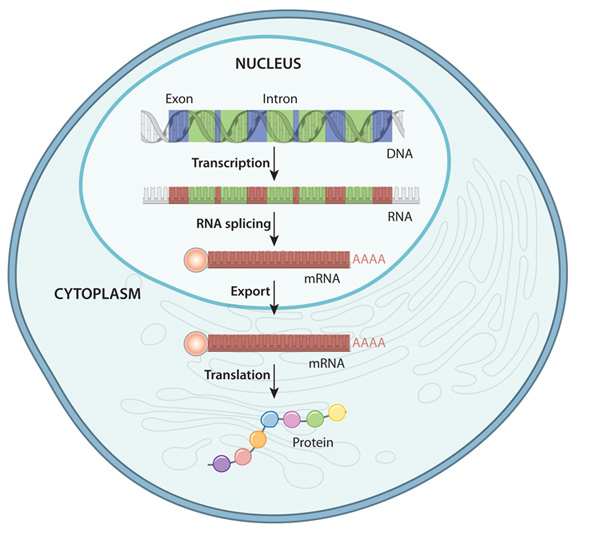
\includegraphics[width=0.8\textwidth]{figures/introduction/gene_expression_process.jpg}
    \caption[Schema of gene expression process]{Overview of gene expression process, from~\cite{cell_essential_nature}}
    \label{fig:gene_expression}
\end{figure}

\subsubsection{RNA maturation}

For the rest of the manuscript, I mainly focus on the \ac{mRNA}s.
They do not fit translation requirements yet and need to undergo three processes before leaving the nucleus:
\begin{itemize}
	\setlength\itemsep{0.1em}
	\item the 5' end is transformed (\ac{RNA} capping)
	\item a poly(A) tail (repeated adenine-based molecules) is added at the 3' end (polyadenylation)
	\item the non-coding parts of the \ac{RNA} sequence are removed (splicing)
\end{itemize}

\noindent
Those transformations enable to move the \ac{mRNA} out of the nucleus, regulate its degradation and promote the translation.
Figure~\ref{fig:gene_expression} shows a simplified illustration of the gene expression process.

%%%%%%%%%%%%%%%%%%%%%%%%%%%%%%%%%%%%%%%%%%%%%%%%%%%%%%%%%%%%%%%%%%%%%%%%%%%%%%%%%%%%%%%%%%%%%%%%%%%%%%%%%%%%%%%%%%%%%%%%%%%%%%%%%%%%%%%%%%%%%%%%%%%%%%%%%%%%
%%%%%%%%%%%%%%%%%%%%%%%%%%%%%%%%%%%%%%%%%%%%%%%%%%%%%%%%%%%%%%%%%%%%%%%%%%%%%%%%%%%%%%%%%%%%%%%%%%%%%%%%%%%%%%%%%%%%%%%%%%%%%%%%%%%%%%%%%%%%%%%%%%%%%%%%%%%%
%%%%%%%%%%%%%%%%%%%%%%%%%%%%%%%%%%%%%%%%%%%%%%%%%%%%%%%%%%%%%%%%%%%%%%%%%%%%%%%%%%%%%%%%%%%%%%%%%%%%%%%%%%%%%%%%%%%%%%%%%%%%%%%%%%%%%%%%%%%%%%%%%%%%%%%%%%%%

\subsection{mRNA transport and localization}
\label{subsec:intro_rna_transport}

When an \ac{mRNA} is ready for export, it is moved out of the nucleus through the nuclear pore complex.
This complex recognizes a mature \ac{mRNA} if a specific set of proteins is bounded to it - poly(a) binding proteins, cap binding proteins, and proteins related to the splicing step.
Once in the cytoplasm, an \ac{mRNA} is not necessarily exploited by a ribosome for translation.
It can also be silenced by translational repressors and stored, transported in a specific region of the cell or degraded.

Until recently, the scientific community thought translation mostly occurred at the endoplasmic reticulum and then proteins were transported where they were needed.
New evidence suggests on the contrary that \ac{mRNA} localization within the cell is not always random and \ac{mRNA}s-proteins colocalization could be an important aspect of cell organization and gene expression regulation~\cite{lecuyer_global_2007}.
However, the involved mechanisms are not well understood yet and the extend of \ac{mRNA}s concerned by a specific localization pattern is still unknown.
Beyond the number of \ac{mRNA} molecules within a cell (the expression level of a gene), researchers manifest now an increasing interest for \ac{mRNA} localization.

\subsubsection{mRNA transport}

Some mechanisms used by the cell to transport or locally enrich \ac{mRNA} have been identified:
\begin{itemize}
	\item Usage of motor proteins to move the \ac{mRNA}s along the cytoskeleton.
	\item Prevention of \ac{mRNA} degradation at a precise location.
	\item Local entrapment to anchor the \ac{mRNA}s.
\end{itemize}

\begin{figure}[]
    \centering
    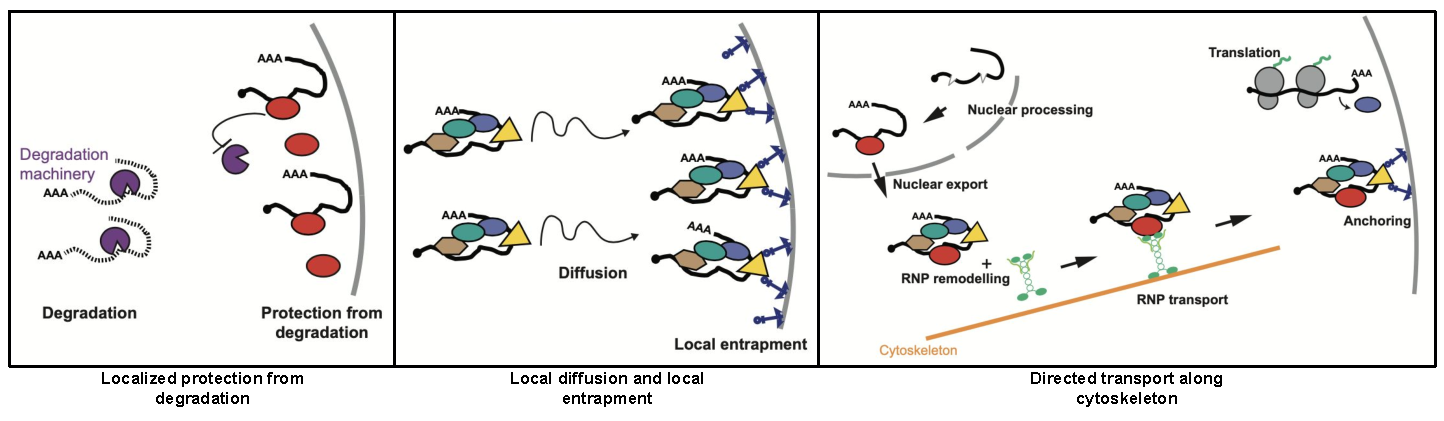
\includegraphics[width=\textwidth]{figures/introduction/rna_transport}
    \caption[Schema of RNA transport or locally enrichment mechanisms]{Schema of RNA transport or locally enrichment mechanisms, adapted from~\cite{Medioni_2012}.
	(\textit{Left}) RNAs are locally protected from degradation.
	(\textit{Center}) RNAs diffuse randomly, then they are locally entrapped.
	(\textit{Right}) RNAs are actively transported along cytoskeleton, thanks to RNP complexes and molecular motors.
	Directed transport can be coupled with an anchoring mechanism}
    \label{fig:rna_transport}
\end{figure}

Figure~\ref{fig:rna_transport}

%%%%%%%%%%%%%%%%%%%%%%%%%%%%%%%%%%%%%%%%%%%%%%%%%%%%%%%%%%%%%%%%%%%%%%%%%%%%%%%%%%%%%%%%%%%%%%%%%%%%%%%%%%%%%%%%%%%%%%%%%%%%%%%%%%%%%%%%%%%%%%%%%%%%%%%%%%%%

%~\cite{Medioni_2012}

% Three distinct mechanisms have been proposed to account for the asymmetric distribution of mRNAs within cells: localized protection from degradation,
% diffusion-coupled local entrapment, and directed transport along a polarized cytoskeleton (Fig. 2).

% Experimentally, distinguishing these mechanisms often requires combining analyses of RNA regulatory sequences with live imaging (Box 1).
% Generalized RNA degradation coupled to local protection has been described in Drosophila, where Hsp83 mRNA is uniformly distributed in early fertilized eggs,
% but restricted to the posteriorly localized germ plasm at later stages (Ding et al., 1993). In the absence of the RNA degradation machinery,
% this selective accumulation is lost and Hsp83 transcripts are stabilized throughout the embryo (Semotok et al., 2005). How the posterior pool of Hsp83 transcripts
% is protected from decay in wild-type conditions is, however, still unclear.
% Localization through diffusion/entrapment has been illustrated for Drosophila nanos mRNA, accumulation of which at the posterior pole of late-stage oocytes
% does not depend on a polarized cytoskeleton, but rather on cortical actin-dependent entrapment and anchoring (Forrest and Gavis, 2003). In early Xenopus oocytes,
% localization of the germ plasm RNAs Xcat2 (Nanos1) and Xdazl has also been proposed to rely on entrapment and association of freely diffusing RNA molecules with
% a densely packed endoplasmic reticulum (ER) concentrated in the vegetally localized mitochondrial cloud (Chang et al., 2004).
% Directed transport of transcripts along a polarized cytoskeletal network is a predominant mechanism to direct mRNA localization (Bullock, 2011) that has been
% observed in a variety of cell types, including Drosophila oocytes and embryos, Xenopus oocytes, migrating mammalian cells and vertebrate neurons (Gagnon and Mowry, 2011).
% A surprising finding from live-imaging analyses (Box 1) was that active motion is not restricted to localizing mRNAs, as uniformly distributed transcripts also undergo
% cytoskeleton-dependent movements (Fusco et al., 2003; Bullock et al., 2006). Rather, the unique feature of localized mRNA movement is that it is non-random, exhibiting
% a net bias explained by increased frequency and duration of directed transport events. How is this net transport achieved? As described below, key

% features appear to involve specific recognition by trans-acting factors, assembly of localization-competent ribonucleoprotein (RNP) complexes, recruitment of molecular
% motors and transport along the cytoskeleton, as well as anchoring of the mRNA at the final destination. Finally, tight coupling with translational regulation
% is required to achieve spatially restricted protein synthesis.

%%%%%%%%%%%%%%%%%%%%%%%%%%%%%%%%%%%%%%%%%%%%%%%%%%%%%%%%%%%%%%%%%%%%%%%%%%%%%%%%%%%%%%%%%%%%%%%%%%%%%%%%%%%%%%%%%%%%%%%%%%%%%%%%%%%%%%%%%%%%%%%%%%%%%%%%%%%%

%~\cite{das_intracellular_2021}

%%%%%%%%%%%%%%%%%%%%%%%%%%%%%%%%%%%%%%%%%%%%%%%%%%%%%%%%%%%%%%%%%%%%%%%%%%%%%%%%%%%%%%%%%%%%%%%%%%%%%%%%%%%%%%%%%%%%%%%%%%%%%%%%%%%%%%%%%%%%%%%%%%%%%%%%%%%%

% aubin thesis

% It is now well appreciated that non-random sub-cellular mRNA localization is important for cellular organization and its misregulation
% is linked to an increasing number of dis- eases [23]. It has been shown that in large and highly polarized cells - like neurons - mRNA localization
% is beneficial for translation. Indeed, it is advantageous for the cell to synthesize the protein at the site of action, rather than at random
% locations in the cytoplasm, requiring thus transport to specific sites [29]. Recent evidence suggests that sub-cellular mRNA localization is
% not restricted to a certain cell or mRNA type, but seems to be generalizable to most cell and mRNAs and is not only linked to local transla- tion [7,12,77].
% It has been shown that central to mRNA localization is an mRNA sequence called zipcode, located mainly in the 3’UTR [18,78]. These zipcodes are recognized
% by RNA-binding proteins (RBP) forming a ribonucleo-protein complex (RNP) when bound
% to the mRNA. The regulation of the transport, translation and degradation of the mRNA is then coordinated by the RBP.
% Active transport and anchorage
% Directed mRNA transport through the cytoskeleton is the predominant mechanism for mRNA localization. Here, the RNP interacts with specific motor proteins via the zipcode [18,78].
% Important examples include the localization of β actin mRNA at the lamelopodia of motile fibroblasts (Fig 1.10, [45]), or the localization of multiple mRNAs in drosophila
% in the apical cytoplasm of epithelial cells [13].
% Selective degradation
% Here, cell locally enrich an mRNA by protecting it from the degradation machinery in a specific location. For instance, it has been shown that HSP83 mRNA
% localizes at the posterior pole of the Drosophilia embryo [6]. However, when the degradation machinery is not functional, this specific localization is
% lost and HSP83 is present uniformly in the embryo [74]. It has been further shown that the RNA degradation is induced by the RNA-binding protein Smaug
% targeting the 3’UTR of the mRNA, again establishing an important link between the 3’UTR and mRNA localization.
% Diffusion and anchorage
% Localization occurs by diffusion of the mRNAs and achoring at a specific cellular com- partment. A well studied example is XCAT2 mRNA which localizes at the
% vegetal cortex (Fig 1.11, [19]).

%%%%%%%%%%%%%%%%%%%%%%%%%%%%%%%%%%%%%%%%%%%%%%%%%%%%%%%%%%%%%%%%%%%%%%%%%%%%%%%%%%%%%%%%%%%%%%%%%%%%%%%%%%%%%%%%%%%%%%%%%%%%%%%%%%%%%%%%%%%%%%%%%%%%%%%%%%%%

% google
% Ribonucleoprotein (RNP) granules are non-membrane bound compartments that form from RNA molecules and
% RNA-binding proteins. Different classes of RNPs carry out diverse roles: for example, some can regulate gene expression while another (the nucleolus) produces ribosomes.

%%%%%%%%%%%%%%%%%%%%%%%%%%%%%%%%%%%%%%%%%%%%%%%%%%%%%%%%%%%%%%%%%%%%%%%%%%%%%%%%%%%%%%%%%%%%%%%%%%%%%%%%%%%%%%%%%%%%%%%%%%%%%%%%%%%%%%%%%%%%%%%%%%%%%%%%%%%%
%%%%%%%%%%%%%%%%%%%%%%%%%%%%%%%%%%%%%%%%%%%%%%%%%%%%%%%%%%%%%%%%%%%%%%%%%%%%%%%%%%%%%%%%%%%%%%%%%%%%%%%%%%%%%%%%%%%%%%%%%%%%%%%%%%%%%%%%%%%%%%%%%%%%%%%%%%%%
%%%%%%%%%%%%%%%%%%%%%%%%%%%%%%%%%%%%%%%%%%%%%%%%%%%%%%%%%%%%%%%%%%%%%%%%%%%%%%%%%%%%%%%%%%%%%%%%%%%%%%%%%%%%%%%%%%%%%%%%%%%%%%%%%%%%%%%%%%%%%%%%%%%%%%%%%%%%

\subsubsection{mRNA localization}

\begin{center}
	\textit{(To be completed)}
\end{center}

%%%%%%%%%%%%%%%%%%%%%%%%%%%%%%%%%%%%%%%%%%%%%%%%%%%%%%%%%%%%%%%%%%%%%%%%%%%%%%%%%%%%%%%%%%%%%%%%%%%%%%%%%%%%%%%%%%%%%%%%%%%%%%%%%%%%%%%%%%%%%%%%%%%%%%%%%%%%

%~\cite{Medioni_2012}

% Transporting mRNAs rather than proteins presents several significant advantages for a cell.
% First, transport costs are reduced, as several protein molecules can be translated from a single RNA molecule.
% Second, transporting mRNAs can prevent proteins from acting ectopically before they reach the appropriate site,
% which is particularly important in the case of maternal determinants, as spatially inappropriate expression disrupts embryonic patterning.
% Third, localized translation can facilitate incorporation of proteins into macromolecular complexes by generating high local
% protein concentrations and allowing co-translation of different subunits (Mingle et al., 2005).
% Fourth, nascent proteins may have properties distinct from pre-existing copies, by virtue of post-translational
% modifications or through chaperone-aided folding pathways (Lin and Holt, 2007).
% Lastly, a major advantage of mRNA targeting is that it allows fine-tuning of gene expression in both space and time.
% Examples of this include targeting of different splice variants to distinct cellular compartments (Baj et al., 2011)
% and activation of localized mRNA translation specifically at their destination, in response to signals
% such as guidance cues, neurotransmitter release or fertilization (Besse and Ephrussi, 2008).

%%%%%%%%%%%%%%%%%%%%%%%%%%%%%%%%%%%%%%%%%%%%%%%%%%%%%%%%%%%%%%%%%%%%%%%%%%%%%%%%%%%%%%%%%%%%%%%%%%%%%%%%%%%%%%%%%%%%%%%%%%%%%%%%%%%%%%%%%%%%%%%%%%%%%%%%%%%%

% chpater 5 intro racha

% Most of \ac{mRNA}s have a random distribution throughout the cytoplasm, but some localize in specific subcellular regions~\cite{Blower_2013, Jung_2014, Eliscovich_2017, Bovaird_2018}.

% Such localization can be related to either \ac{RNA} metabolism, for example with untranslated \ac{mRNA}s stored and repressed in \ac{P-bodies} (but not degraded~\cite{Hubstenberger_2017}), or  protein metabolism with locally translated proteins.
% This local synthesis concerns both mature proteins and nascent peptides.
% Different cellular processes imply the delivery of mature proteins in specific subcellular regions and a local regulation of the proteome.
% Local translation can contributes to cell fate determination during metazoan development, as observed in~\cite{melton_translocation_1987} with a clear modification of the Vg1 \ac{RNA} spatial distribution between mature and immature Xenopus oocytes.
% In mammalian cells, \ac{RNA} localization influences cell polarization and motility, usually through actin localization at the cell edge~\cite{Lawrence_1986}.
% Locally translated proteins are also known to be involved in axonal growth and so neural plasticity~\cite{VanDriesche_2018}.
% Finally, by precisely controlling the \ac{mRNA} localization and the subsequent translation process, cells can avoid to release proteins at inappropriate places~\cite{Muller_myelin_2013} and help the synthesis of protein complexes~\cite{pichon_visualization_2016}.

% Several mechanisms drive the localization of \ac{mRNA}s.
% Sometimes the nascent peptide can serve as a targeting signal, but most of the time the \ac{RNA} molecule itself will initiate its localization.
% The molecule often include a zip-code sequence that is read by a \ac{RBP} and starts the assembly of a transport complex comprising different organelles or motor proteins.
% Such complex can then directly transport the \ac{RNA} along the cytoskeleton~\cite{Blower_2013}.
% Coupled with an anchoring mechanism at the targeted destination, it provides a better stability of the \ac{RNA} localization.
% Following a random diffusion across the cell, a transcript can also be trapped in specific subcellular compartments.
% Likewise, a local protection from degradation will bias the \ac{RNA} spatial distribution.

%%%%%%%%%%%%%%%%%%%%%%%%%%%%%%%%%%%%%%%%%%%%%%%%%%%%%%%%%%%%%%%%%%%%%%%%%%%%%%%%%%%%%%%%%%%%%%%%%%%%%%%%%%%%%%%%%%%%%%%%%%%%%%%%%%%%%%%%%%%%%%%%%%%%%%%%%%%%

% thesis adham

%2. mRNA localization in cell lines: generalities
%The two mRNA localization screens provided insights into general mRNA localization features in cell lines:

%First, even in the case of mRNAs that produce a strong pattern (DYNC1H1 mRNAs localizing in foci for example), a non-negligible fraction of mRNA molecules
% always seems to have random distribution. This is not the case in other systems such as developing embryos or oocytes in which most molecules of a
% localized transcript actually display the pattern. The reasons behind this difference are unclear; but (i) they could be a general aspect of mRNA
% localization in cell lines, in which they are much less stereotyped than embryos, especially cancer ones like HeLa; (ii) they could arise due to
% the relatively smaller size of HeLa cells (although similar observations are made in neurons which argues against this); (iii) localizing only a
% fraction of mRNA molecules is sufficient to carry out the intended biological function (discussed in detail below), in which there is no need to
% localize all transcripts for the cell to function properly.

%mRNA localization occurs in a wide range of subcellular locations in cell lines. These include cellular protrusions, the Golgi apparatus,
% endosomes, the nuclear envelope, cell edges, centrosomes, and even the cytosolic space itself (as in the case of mRNA foci and polarized distributions).
% This demonstrates the variety of mRNA trafficking and the diverse functions of mRNA localization.

%Most localized mRNAs display ìsimpleî localization patterns in which they belong to one of the described localization classes (intranuclear, nuclear envelope,
% cell edge, cell extension, polarized, foci, centrosomes). However, some transcripts show ìcomplexî patterns in which they localize to multiple compartments
% either simultaneously or at different times. An example of this is HMMR mRNA that localizes to both centrosomes and P-bodies during interphase.
% This difference is probably related to the function of each transcript but it implies that mRNA localization can be complex and can involve multiple
% sub-cellular compartments at once (see ASPM below for a detailed example).

%mRNA localization often exhibits cellular heterogeneity. Indeed, not all cells exhibit the pattern, and the strength of the pattern could vary between cells that display it.
% The is probably related to:
% (i) cells having different physiological states and thus different gene expression needs;
% (ii) cells being in different stages of the cell cycle;
% (iii) variations in mRNA
%expression levels; (iv) variation in motors protein availability, RBP expression, cytoskeletal arrangements; or (v) a stochastic process yet unidentified.

%3. A variety of local translation flavors
% In many cases, mRNAs co-localized with the protein they encode suggesting local translation. This was observed in a variety of regions such as cell extensions,
% cell edges, centrosomes, endosomes, and the Golgi network. Local translation could function in:

% Protein targeting: ASPM mRNA for instance was the first case of local translation at the nuclear pore during interphase and this could facilitate nucleoplasmic
% targeting of the mature ASPM protein.

% Preventing aberrant dispersal of proteins that could have harmful effects. For example, NUMA1 mRNA and protein are only localized on centrosomes during mitosis.
% Targeting NUMA1 protein to centrosomes during interphase could have deleterious effects.

% Enhancing translation efficiencies: this applies to mRNAs that are localized and translated in cytoplasmic foci referred to as translation factories.
% These structures could host an environment more suitable for translation (a more favorable concentration of translation factors for instance).
% In fact, DYNC1H1 mRNAs are translated as both single molecules and mRNA foci. However, mRNAs in the foci are more often found engaged in translation than ones that
% exist as single molecules. Here, it is tempting to speculate that translation factories harbor specialized ribosomes or components of the translation machinery that
% are dedicated for localized cases of protein synthesis.

% Nascent peptide metabolism: synthesizing components of a protein complex locally can enhance the efficiency of complex assembly for example. Another possibility
% is co- translational assembly at certain organelles. For instance, translating mRNAs encoding centrosomal proteins such as PCNT, CEP350, NIN, and HMMR could help
% to incorporate the mature protein into centrosomes during the expansion of the pericentriolar material that occurs during the late G2 phase of the cell cycle.
% Finally, local translation could allow certain

%%%%%%%%%%%%%%%%%%%%%%%%%%%%%%%%%%%%%%%%%%%%%%%%%%%%%%%%%%%%%%%%%%%%%%%%%%%%%%%%%%%%%%%%%%%%%%%%%%%%%%%%%%%%%%%%%%%%%%%%%%%%%%%%%%%%%%%%%%%%%%%%%%%%%%%%%%%%
%%%%%%%%%%%%%%%%%%%%%%%%%%%%%%%%%%%%%%%%%%%%%%%%%%%%%%%%%%%%%%%%%%%%%%%%%%%%%%%%%%%%%%%%%%%%%%%%%%%%%%%%%%%%%%%%%%%%%%%%%%%%%%%%%%%%%%%%%%%%%%%%%%%%%%%%%%%%
%%%%%%%%%%%%%%%%%%%%%%%%%%%%%%%%%%%%%%%%%%%%%%%%%%%%%%%%%%%%%%%%%%%%%%%%%%%%%%%%%%%%%%%%%%%%%%%%%%%%%%%%%%%%%%%%%%%%%%%%%%%%%%%%%%%%%%%%%%%%%%%%%%%%%%%%%%%%

\subsection{Translation}
\label{subsec:intro_translation}

Finally, a cell synthesizes a protein through the translation process.
A ribosome is assembled around a \ac{mRNA} and moves along its nucleotides.
At the same time, \ac{tRNA}s carry amino acids matching the \ac{mRNA} sequence.
According to the genetic code, three successive nucleotides of the \ac{mRNA} (a codon) correspond to an amino acid.
The ribosome sequentially chains the amino acids, which then fold into a functional protein with a specific 3-dimensional structure.

%%%%%%%%%%%%%%%%%%%%%%%%%%%%%%%%%%%%%%%%%%%%%%%%%%%%%%%%%%%%%%%%%%%%%%%%%%%%%%%%%%%%%%%%%%%%%%%%%%%%%%%%%%%%%%%%%%%%%%%%%%%%%%%%%%%%%%%%%%%%%%%%%%%%%%%%%%%%
%%%%%%%%%%%%%%%%%%%%%%%%%%%%%%%%%%%%%%%%%%%%%%%%%%%%%%%%%%%%%%%%%%%%%%%%%%%%%%%%%%%%%%%%%%%%%%%%%%%%%%%%%%%%%%%%%%%%%%%%%%%%%%%%%%%%%%%%%%%%%%%%%%%%%%%%%%%%
%%%%%%%%%%%%%%%%%%%%%%%%%%%%%%%%%%%%%%%%%%%%%%%%%%%%%%%%%%%%%%%%%%%%%%%%%%%%%%%%%%%%%%%%%%%%%%%%%%%%%%%%%%%%%%%%%%%%%%%%%%%%%%%%%%%%%%%%%%%%%%%%%%%%%%%%%%%%

\section{Imaging cells and RNAs}
\label{sec:fish}

\begin{figure}[]
    \centering
    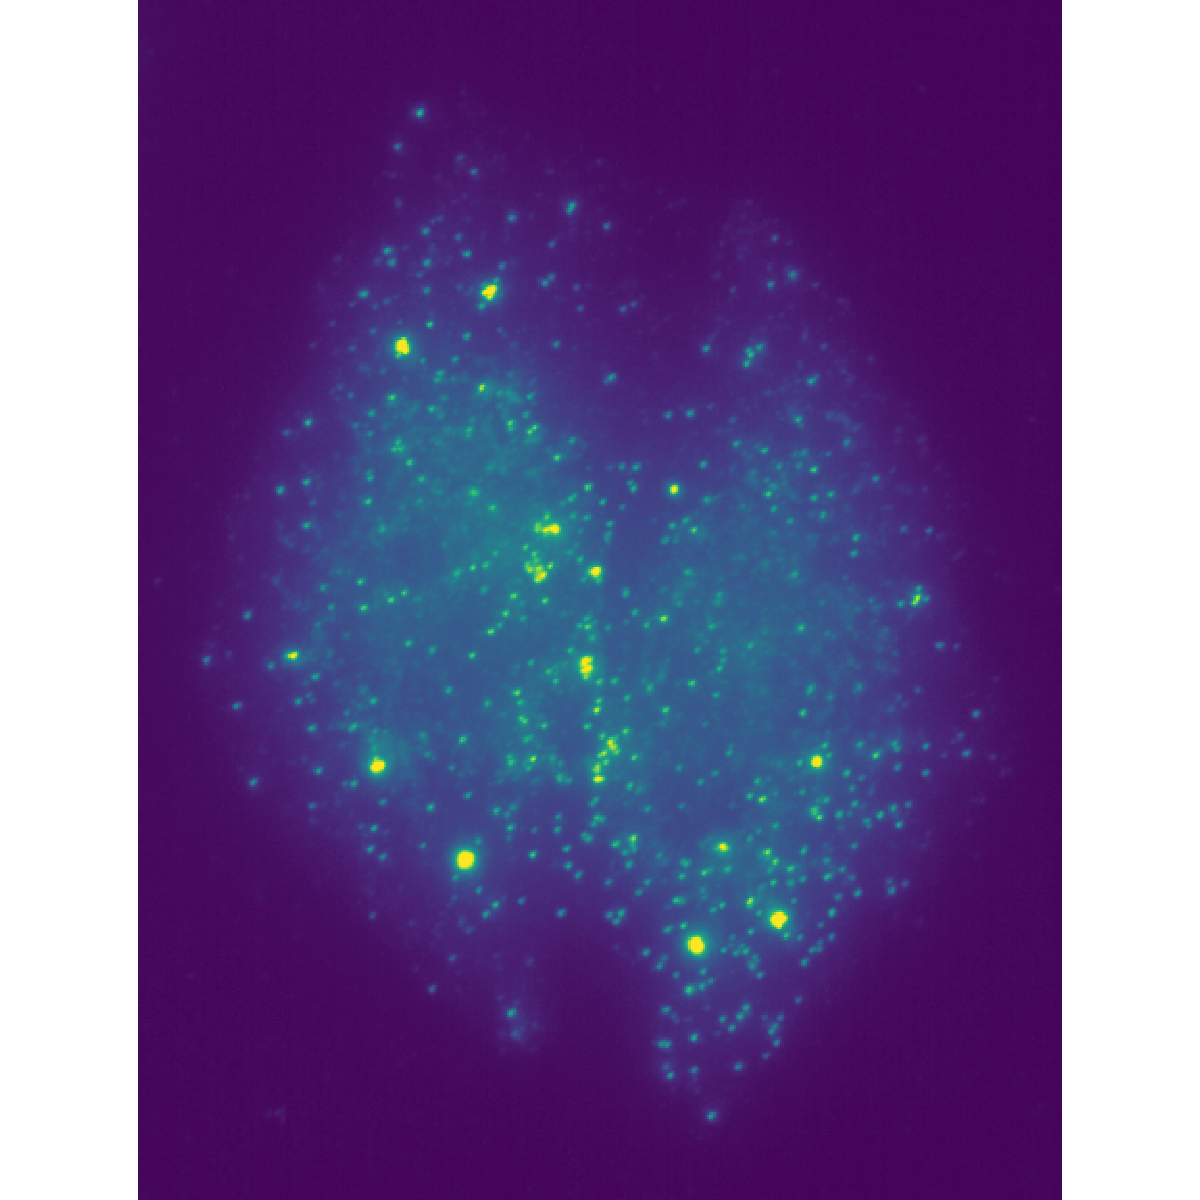
\includegraphics[width=\textwidth]{figures/introduction/multichannel_input}
    \caption[Example of DAPI and smiFISH images]{Example of DAPI (\textit{left}) and smiFISH (\textit{right}) images}
    \label{fig:multichannel_input}
\end{figure}

\subsection{Fluorescent proteins}
\label{subsec:intro_fluorescence}

\begin{center}
	\textit{(To be completed)}
\end{center}

\subsection{A zoo of FISH}
\label{subsec:intro_fish}

\begin{center}
	\textit{(To be completed)}
\end{center}

%%%%%%%%%%%%%%%%%%%%%%%%%%%%%%%%%%%%%%%%%%%%%%%%%%%%%%%%%%%%%%%%%%%%%%%%%%%%%%%%%%%%%%%%%%%%%%%%%%%%%%%%%%%%%%%%%%%%%%%%%%%%%%%%%%%%%%%%%%%%%%%%%%%%%%%%%%%%

% thesis adham: "the invention of single molecule FISH (Femino et al., 1998)"
% ~\cite{Femino_1998}

%%%%%%%%%%%%%%%%%%%%%%%%%%%%%%%%%%%%%%%%%%%%%%%%%%%%%%%%%%%%%%%%%%%%%%%%%%%%%%%%%%%%%%%%%%%%%%%%%%%%%%%%%%%%%%%%%%%%%%%%%%%%%%%%%%%%%%%%%%%%%%%%%%%%%%%%%%%%

% paper racha (dual protein-rna localization screens)

% In order to simultaneously visualize mRNAs with their encoded proteins, we based our screen on a library of HeLa cell lines,
% each containing a bacterial artificial chromosome (BAC) stably integrated in their genome (Poser et al., 2008).
% Each BAC con- tains a GFP-tagged gene harboring all its regulatory sequences (promoter, enhancers, introns, and 50 and 30 UTRs; Figure 1A).
% The resulting mRNAs are, thus, identical to the endogenous mol- ecules in terms of sequence and isoform diversity, except for the added tag.
% Previous studies showed that such tagged genes are expressed at near endogenous levels and with the proper spatio- temporal pattern (Poser et al., 2008).
% Since the tagged mRNAs contain all the regulatory sequences, we hypothesized that they would localize like the endogenous ones,
% provided that the tag does not interfere with localization. Using BACs offers two advantages. First, a single smFISH probe set
% against the GFP sequence is sufficient to detect all the studied mRNAs. Sec- ond, using mild hybridization conditions,
% GFP fluorescence can be detected together with the smFISH signal (Fusco et al., 2003), and thus, both the mRNA and the encoded protein can be detected in the same cell.

%%%%%%%%%%%%%%%%%%%%%%%%%%%%%%%%%%%%%%%%%%%%%%%%%%%%%%%%%%%%%%%%%%%%%%%%%%%%%%%%%%%%%%%%%%%%%%%%%%%%%%%%%%%%%%%%%%%%%%%%%%%%%%%%%%%%%%%%%%%%%%%%%%%%%%%%%%%%

\begin{wrapfigure}{R}{0.60\textwidth}
	\begin{center}
	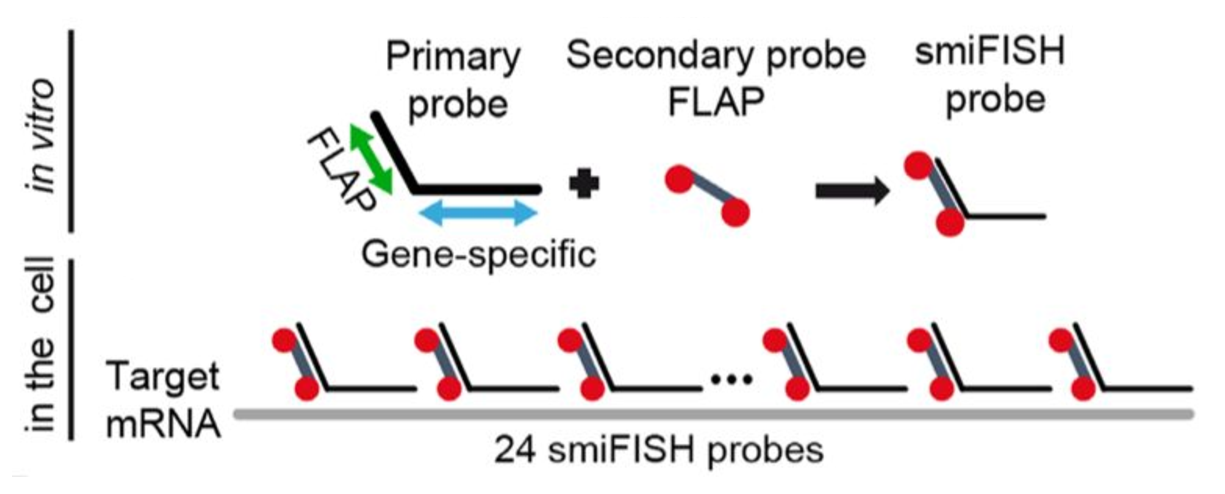
\includegraphics[width=\linewidth]{figures/introduction/smiFISH}
	\caption[Schema of smiFISH protocol]{Schema of smiFISH protocol from~\cite{tsanov_smifish_2016}}
	\label{fig:smiFISH}
	\end{center}
\end{wrapfigure}

%%%%%%%%%%%%%%%%%%%%%%%%%%%%%%%%%%%%%%%%%%%%%%%%%%%%%%%%%%%%%%%%%%%%%%%%%%%%%%%%%%%%%%%%%%%%%%%%%%%%%%%%%%%%%%%%%%%%%%%%%%%%%%%%%%%%%%%%%%%%%%%%%%%%%%%%%%%%
%%%%%%%%%%%%%%%%%%%%%%%%%%%%%%%%%%%%%%%%%%%%%%%%%%%%%%%%%%%%%%%%%%%%%%%%%%%%%%%%%%%%%%%%%%%%%%%%%%%%%%%%%%%%%%%%%%%%%%%%%%%%%%%%%%%%%%%%%%%%%%%%%%%%%%%%%%%%
%%%%%%%%%%%%%%%%%%%%%%%%%%%%%%%%%%%%%%%%%%%%%%%%%%%%%%%%%%%%%%%%%%%%%%%%%%%%%%%%%%%%%%%%%%%%%%%%%%%%%%%%%%%%%%%%%%%%%%%%%%%%%%%%%%%%%%%%%%%%%%%%%%%%%%%%%%%%

\section{Measuring images: from pixels to numbers}
\label{sec:computation_biology}

\subsection{Working with bioimages}
\label{subsec:intro_bioimages}

Recent developments in life sciences and technological breakthroughs greatly increase the importance of quantitative approaches.
A typical example is the Human Genome Project~\cite{lander_initial_2001} that aims to decipher human genome by the use of novel sequencing techniques.
Data collection and maintenance, as well as development of methods to extract valuable insights from it, is transforming biology in depth.
Current experimental platforms allow us to perform a large number of experiments under varied conditions and highly informative content.
These techniques are referred as High Content Screening and pave the way for a systematic analysis of living systems.
Finally, the increasing degree of automation of experimental protocols justifies the development of bioinformatics as a discipline in its own right to assist biologists.

The use of images in biology brings several advantages.
It enables the study of morphological patterns that could subsequently be related to phenotypes.
It also preserves the spatial dimension of the living system studied, as well as its temporal dimension in the case of repeated image acquisitions or live imaging experiments.
Last but not least, an analysis can be performed at different scales, from the molecule to the whole organ, through the tissues.
Overall, the tasks addressed with these bioimages can be
In general, the tasks performed with these bioimages can be as varied as the visualization of a living system, the reconstruction of a microscopy images, its denoising or the recognition of specific phenotypes.

One word to summarize bioimages would be \emph{heterogeneity}.
A living system can be imaged at different scales, with different modalities of acquisition and evolving technology.
In addition, the fluorescent markers used in microscopy or the question investigated by researcher could differ, making images of the same object from two different studies not necessarily compatible.
As a consequence, the subsequent computational analysis should be adapted for one set of images to another.

\subsection{Machine learning for bioimages}
\label{subsec:intro_ml_tools}

\subsubsection{A machine learning boom}

The recent years have seen a renewed interest for machine learning research, the cornerstone of current artificial intelligence era, driven by successful applications in vision, language understanding, speech recognition, etc\dots
This term of machine learning was coined to describe the set of techniques and models that make automatic decision based on patterns \emph{learned} and found in data.
For some specific tasks (like image classification) these algorithms have reached human-like capabilities.
For other fields, the gap between computer and human performances keeps decreasing.
In computer vision, the success of machine learning models makes their use legitimate for bioinformatics applications.\\

\noindent
Overall, three ingredients make these successes possible:
\begin{enumerate}
	\setlength\itemsep{0.1em}
	\item models fitted with learning algorithms
	\item large annotated datasets
	\item increased computing power to process an ever growing number of operations
\end{enumerate}

\noindent
The first ingredient is not necessarily new.
Machine learning and deep learning models (a family of machine learning models based on artificial neural networks), as well as learning algorithms have been studied and developed for decades (see~\cite{Bishop_2006, Tibshirani_2009} for a review of different machine learning methods).
As a symbol, the release of a large dataset with manual annotations for natural image classification problem~\cite{Deng_2009}, followed by a breakthrough performance with a \ac{CNN}~\cite{alexnet_2012}, marks the beginning of a new era for deep learning.
Obviously, the impact of these models has been consequent for every computational field.
In biomedical community, machine learning techniques are disseminating and address more challenges every year (see~\cite{jumper_highly_2021} for an example with the protein folding problem).

\subsubsection{Neural networks as the next generation tool}

In case of deep learning, model architecture is based on a neural network with successive layers of artificial neurons.
Each neuron is defined by a set of weights and perform a linear combination of the input signal with its weights, followed by a potential non linear transformation (usually a \emph{maxout}, \emph{sigmoid} or \emph{tanh} function).
A complete network usually combines these layers of neurons with normalization steps.
It can be seen as a parametrized model, whose weights need to be optimized to minimize for a specific task.

Given an input, a loss function enables to compare the output signal of the model with a ground truth (the expected output signal) and thus compute a gradient (the first order derivative of the loss function).
The backpropagation of this gradient to the rest of the network makes it possible to update the weights of the layers in order to minimize the loss~\cite{rumelhart_learning_1986}.
This process defines a training step.
After several iterations, the loss and the gradient should decrease, and the network progressively stabilizes its weights.
The weights are ultimately frozen and the model is trained.

Such architecture is highly flexible and different variants have been developed, with convolutional or recurrent layers to name a few~\cite{lecun_deep_2015}.
For a general introduction to deep learning techniques, one can refer to~\cite{Goodfellow_2016}.

\subsubsection{Limitations and caveats}

Beyond the great performances returned by machine learning models, a number of limitations and caveats should be consider.

First, they require annotated datasets to train and evaluate the models.
Compare to natural images, this ground truth is particularly costly to obtained with biomedical images as it often involves the assignation of experts (medical doctor or biologists) to a time-consuming, repetitive and annoying task.
As a consequence, datasets available for a given biomedical problem are often too small, highly diversified or released without any useful manual annotations.

Second, machine learning algorithms require robust evaluation protocol, strong benchmarks and a rigorous choice of evaluation metrics\footnote{One can see~\cite{varoquaux_machine_2022} for a description of these evaluation caveats when machine learning models are applied to medical images.}.
It is necessary to prevent data leakage and firmly separate the train set from the test set in our dataset, otherwise models overfit to the training samples and badly generalize to unknown data.
If the test set is not representative of the data distribution, or too small, the evaluation will be biased and hardly reproducible~\cite{Varoquaux_cv_2018}.
Obviously, all these limitations are worsen by the inherent heterogeneity of bioimages and the difficulty to assemble manual annotations.
Working with machine learning models, one needs strong and diversified baselines that reflect the state-of-the-art of performances, as well as the right choice of metrics to compare his methods to the rest of the literature.

Third, flexibility of some models comes at a price: a sensitivity to the selected hyperparameters, which makes the evaluation all the more important.

Last but not least, most of the deep learning models appear like a black box solution with an internal process that cannot be easily or directly interpreted.
If this problem is more critical for direct medical applications than biological ones, yet it requires an important pedagogical effort to diffuse deep learning techniques to the rest of the scientific community.

\section{Goals and contributions}
\label{sec:contributions}

\subsection{Goals}
\label{subsec:intro_goals}

\begin{figure}[]
	\centering
	\minipage{0.2\textwidth}
		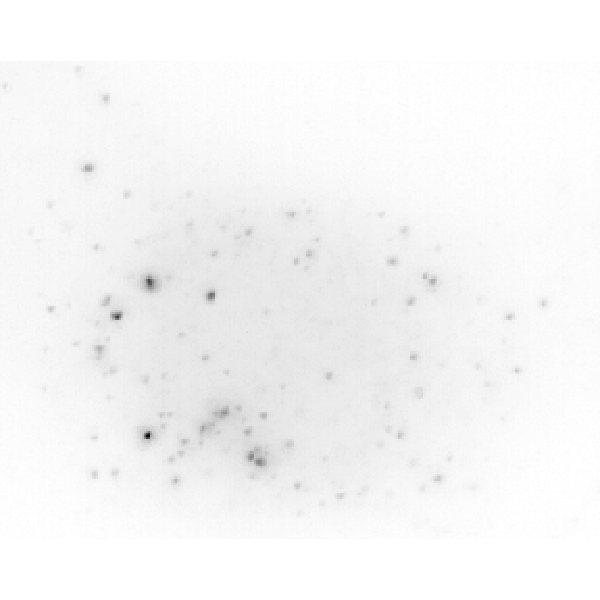
\includegraphics[width=0.95\linewidth]{figures/introduction/real_image_foci}
		\vfill
		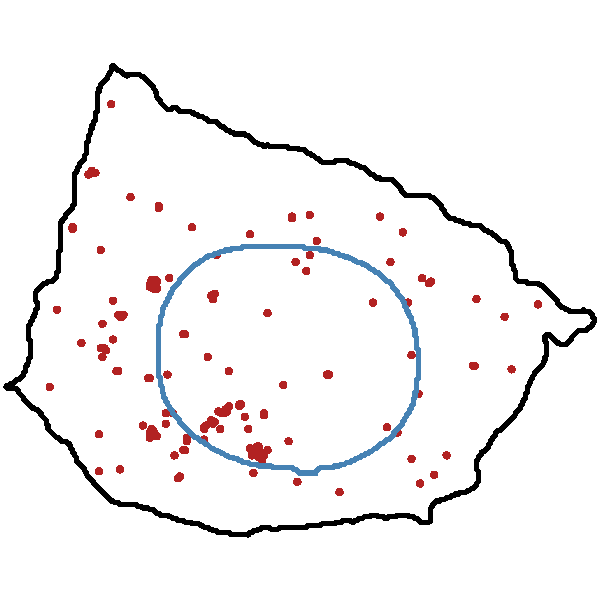
\includegraphics[width=0.95\linewidth]{figures/introduction/real_coord_foci}
		\subcaption{Foci}
	\endminipage\hfill
	\minipage{0.2\textwidth}
		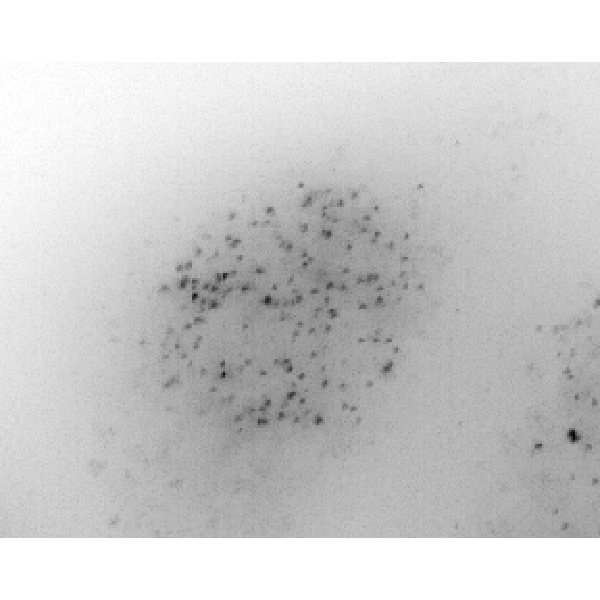
\includegraphics[width=0.95\linewidth]{figures/introduction/real_image_intranuclear}
		\vfill
		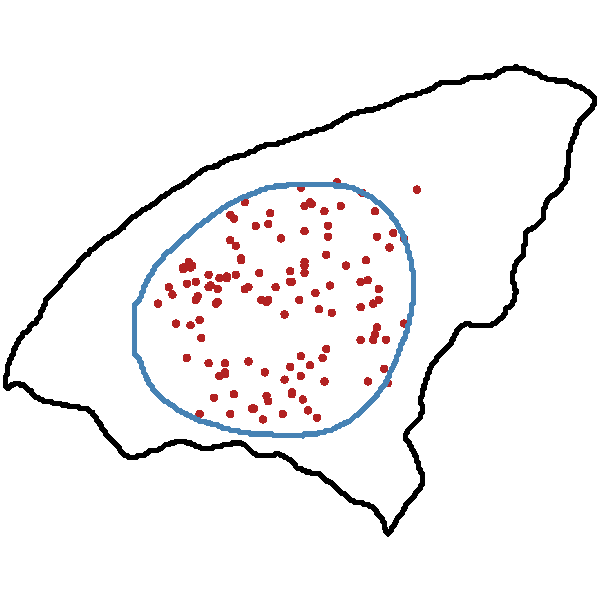
\includegraphics[width=0.95\linewidth]{figures/introduction/real_coord_intranuclear}
		\subcaption{Intranuclear}
	\endminipage\hfill
	\minipage{0.2\textwidth}
		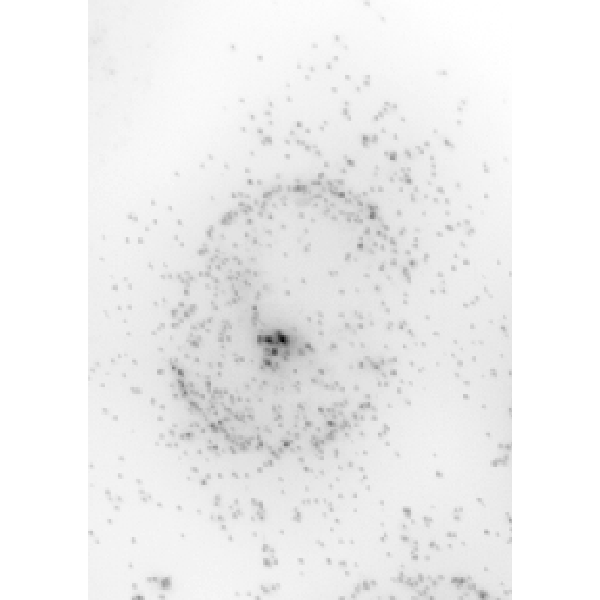
\includegraphics[width=0.95\linewidth]{figures/introduction/real_image_nuclear_edge}
		\vfill
		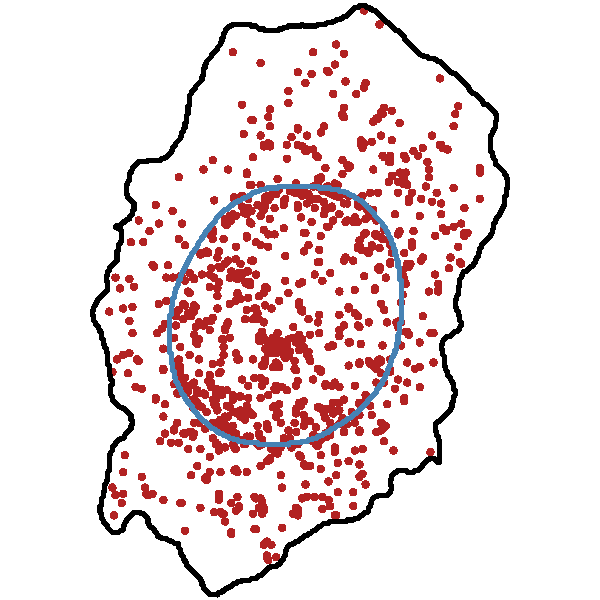
\includegraphics[width=0.95\linewidth]{figures/introduction/real_coord_nuclear_edge}
		\subcaption{Nuclear edge}
	\endminipage\hfill
	\minipage{0.2\textwidth}
		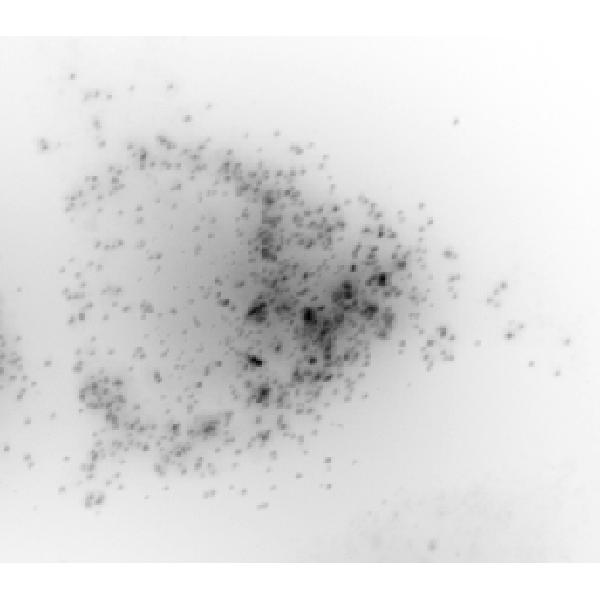
\includegraphics[width=0.95\linewidth]{figures/introduction/real_image_perinuclear}
		\vfill
		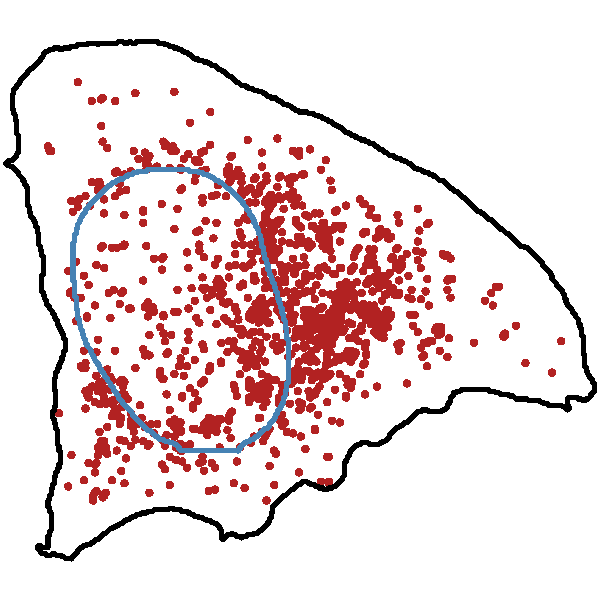
\includegraphics[width=0.95\linewidth]{figures/introduction/real_coord_perinuclear}
		\subcaption{Perinuclear}
	\endminipage\hfill
	\minipage{0.2\textwidth}
		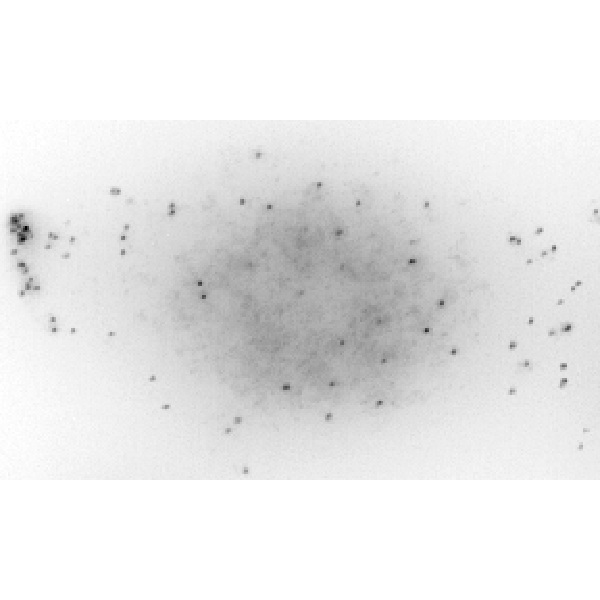
\includegraphics[width=0.95\linewidth]{figures/introduction/real_image_protrusion}
		\vfill
		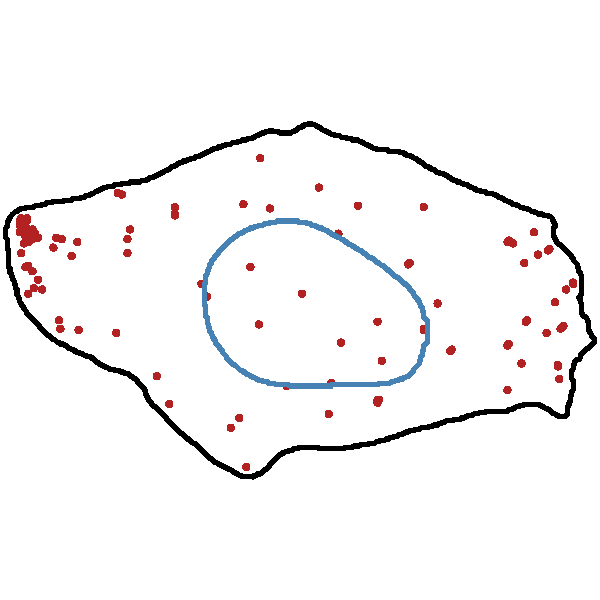
\includegraphics[width=0.95\linewidth]{figures/introduction/real_coord_protrusion}
		\subcaption{Protrusion}
	\endminipage
	\caption[RNA localization patterns from pixels to numbers]{RNA localization patterns from~\cite{pointfish_2022}.
	(\textit{Top}) Typical smFISH images with different RNA localization patterns.
	(\textit{Bottom}) Coordinate representations with RNA spots (\textit{red}), cell membrane (\textit{black}) and nuclear membrane (\textit{blue}).
	Detection and segmentation results are extracted and visualized with FISH-quant~\cite{Imbert_fq_2022}}
	\label{fig:intro_localization_patterns}
\end{figure}

At the beginning of my PhD, three main goals were defined with my supervisors.
The first one was the development and the implementation of a complete pipeline to process \ac{smFISH} images and return valuable insights about \ac{RNA} localization.
In particular, it was expected to integrate and adapt the latest successful developments in computer vision.
Figure~\ref{fig:intro_localization_patterns} illustrates the gap that needs to be bridged between the input images and an adequate representation of the \ac{RNA} localization, making their quantitative analysis possible.
The second goal was the identification of bottlenecks that would prevent scaling the analysis to thousands images, in high content screening assays.
Such bottlenecks should be minimized or solved during the thesis to be able to scale any computational analysis based on \ac{smFISH} experiments.
Lastly, this complete framework would be applied to real experimental datasets in ongoing biological studies.

\subsection{Contributions}
\label{subsec:intro_contributions}

Beyond this own manuscript, my contributions are essentially lines of code.
With a effort of transparency, reproducibility and documentation, I try to develop computational tools as useful as possible for any biologist interested in \ac{FISH} experiments.
My PhD results in three major contributions.

\begin{itemize}
	\setlength\itemsep{0.1em}
	\item My first and main contribution is FISH-quant V2.
	This online framework gathers Python packages and a \ac{GUI} to process \ac{FISH} images, build robust analysis pipelines and even perform simulations.
	\item My second important contribution is an alternative method to compute relevant features in order to discriminate \ac{RNA} localization patterns.
	This method implies the development of PointFISH, a dedicated deep learning model for point cloud.
	\item My third contribution is my participation to biological studies with meaningful results.
	These studies leveraged high content screening assays and \ac{smFISH} techniques to perform a systemic analysis of \ac{RNA} localization and investigate local translation phenomenons.
\end{itemize}

\noindent
Some other contributions are also mentioned throughout this manuscript.
It includes a dataset I annotated for nucleus and cell segmentation with thousands of instances and my supervision of an intern.
The work performed during this internship was the seed for the first publication of another PhD student in the team, about in silico labeling and segmentation.
Lastly, a list of my publications are available at the very end of the manuscript.

\subsection{Manuscript summary}
\label{subsec:intro_manuscript}

The manuscript is composed of two parts.
The first four chapters are a presentation of the analysis pipeline with a focus on every critical stage.
It includes systematic reviews of the existing methods and details about solutions I implemented.
In addition, code snippets, ready to be imported and run, are interspersed with descriptions of the related algorithms.
The second part details several applications of my tools, where quantification of \ac{RNA} localization patterns supports biological insights.

In \textbf{Chapter~\ref{ch:chapter1}}, I present the general computational framework I developed and published: FISH-quant v2.
It includes methods for every stages of a \ac{FISH}-based analysis, with an effort to make them scalable and modular.
I also describe the improvements from the original FISH-quant version, and how it addresses the requirements of a modern software tool.

In \textbf{Chapter~\ref{ch:chapter2}}, I focus on the \ac{RNA} detection stage.
With \ac{smFISH} experiments, the \ac{RNA} molecules are spotted and reduced to discrete data points in space.
I describe detection algorithms and their extensions available in FISH-quant.
In the end, the set of all \ac{RNA} molecules is reduced to a point cloud with spatial coordinates.

In \textbf{Chapter~\ref{ch:chapter3}}, I review and describe algorithms for nucleus and cell segmentation.
Most of them are deep learning models, trained on vast datasets of annotated images.
Beside my own implemented methods, I also present refinement techniques to improve and format segmentation masks.
Two other projects for which I contributed (including one published) are also discussed at the end of the chapter.
They aim at improving the efficiency and consistency of segmentation on specific aspects.

In \textbf{Chapter~\ref{ch:chapter4}}, I compare two different approaches to quantify \ac{RNA} localization patterns.
Once the \ac{RNA} molecules are detected and cell morphology is segmented, the pixel domain gives way to Euclidean space and cells can be represented with a coordinate representation.
Then, spatial features are computed in order to discriminate relevant localization pattern.
I present two different methods of feature engineering.
The first method consists in manually designing features to characterize specific localization patterns.
I then list and describe every hand-crafted feature implemented in FISH-quant.
The second (published) method consists in learning features.
They are extracted from a deep learning model fed with the \ac{RNA} point cloud as input and trained on a simulated pretext task.

In \textbf{Chapter~\ref{ch:chapter5}}, I present several applications of my quantitative pipeline.
These applications come from three publications where we study different \ac{RNA} localization patterns and cases of local translation.
My analyses support and validates biological insights claimed in these studies about \ac{RNA} localization.
I design a classification pipeline to recognize generic localization patterns.
I evaluate the impact of translation inhibitor on \ac{RNA} localization and help identifying a singular translation-dependent pattern.
I quantify a cell cycle dependent pattern, which is related to centrosomes.
Finally, I also contribute to a a study focused on the protrusion pattern.

%%%%%%%%%%%%%%%%%%%%%%%%%%%%%%%%%%%%%%%%%%%%%%%%%%%%%%%%%%%%%%%%%%%%%%%%%%%%%%%%%%%%%%%%%%%%%%%%%%%%%%%%%%%%%%%%%%%%%%%%%%%%%%%%%%%%%%%%%%%%%%%%%%%%%%%%%%%%
%%%%%%%%%%%%%%%%%%%%%%%%%%%%%%%%%%%%%%%%%%%%%%%%%%%%%%%%%%%%%%%%%%%%%%%%%%%%%%%%%%%%%%%%%%%%%%%%%%%%%%%%%%%%%%%%%%%%%%%%%%%%%%%%%%%%%%%%%%%%%%%%%%%%%%%%%%%%
%%%%%%%%%%%%%%%%%%%%%%%%%%%%%%%%%%%%%%%%%%%%%%%%%%%%%%%%%%%%%%%%%%%%%%%%%%%%%%%%%%%%%%%%%%%%%%%%%%%%%%%%%%%%%%%%%%%%%%%%%%%%%%%%%%%%%%%%%%%%%%%%%%%%%%%%%%%%

% plots

% (RNA maturation)
% RNA transport mechanism

% smFISH + microscope
% multichannel images (dapi + smfish)
% multiplexed FISH

% (deep learning architecture)

% add presentation of the localization patterns (from pixel to coord + patterns)
% mention Weeks et al. (1985) as firstpublication about RNA localization
% adham thesis: "Messenger localization was first discovered in Xenopus oocytes (Weeks et al., 1985)."


%%%%%%%%%%%%%%%%%%%%%%%%%%%%%%%%%%%%%%%%%%%%%%%%%%%%%%%%%%%%%%%%%%%%%%%%%%%%%%%%%%%%%%%%%%%%%%%%%%%%%%%%%%%%%%%%%%%%%%%%%%%%%%%%%%%%%%%%%%%%%%%%%%%%%%%%%%%%

% paper racha (introduction)

%how
%- rna metabolism
%- protein metabolism (mature protein or nascent protein)

%why
%- storage of untranslated rna
%- local translation
%- rapid cell division cycle (linked to local translation of cyclin B mRNAs)
%- cell polarization
%- cell motility (actin at the leading edge)
%- axonal growth and synaptic plasticity of neurons
%- assembly of protein complexes
%- avoid proteins in wrong place

%how
%- targeting signal of nascent protein
%- targeting from rna zip-code sequence (with RNA-binding proteins)
%- direct transport on the cytoskeleton by molecular motors
%- anchoring mechanism
%- diffusion, trapping, degradation and local rna stabilization

%claim
%- lack a global view of local translation in the entire cellular space or at the genomic level
%- need a systematic manner

%examples
%- pioneering study in Drosophila
%- human cell lines

%limitations
%- information on RNA localization but did not directly investigate local translation as the encoded proteins were not detected

%%%%%%%%%%%%%%%%%%%%%%%%%%%%%%%%%%%%%%%%%%%%%%%%%%%%%%%%%%%%%%%%%%%%%%%%%%%%%%%%%%%%%%%%%%%%%%%%%%%%%%%%%%%%%%%%%%%%%%%%%%%%%%%%%%%%%%%%%%%%%%%%%%%%%%%%%%%%

% paper racha (introduction)

% Most mRNAs are distributed randomly throughout the cytoplasm, but some localize to specific
% subcellular areas (Blower, 2013; Bovaird et al., 2018; Eliscovich and Singer, 2017; Jung et al., 2014 for reviews).

% This phenomenon is linked to either RNA metabolism, when untranslated mRNAs are stored in P- bodies or other cellular structures (Hubstenberger et al., 2017),
% or to protein metabolism, when a protein is synthesized locally.

% Local translation has been observed from bacteria and yeast to humans (Blower, 2013; Jung et al., 2014; Eliscovich and Singer, 2017; Bovaird et al., 2018).

% It is commonly involved in the delivery of mature proteins to specific cellular compartments, while allowing local regulation, and this is involved in many processes.
% For instance, it contributes to patterning and cell fate determination during metazoan development, mainly through asymmetric cell division
% (Melton, 1987; Driever and Nu€sslein- Volhard, 1988).
% In Xenopus embryos, local translation of cyclin B mRNAs at the mitotic spindle is also believed to be important for the rapid cell
% division cycles occurring during early embryo- genesis (Groisman et al., 2000).
% In mammals, mRNA localization is involved in cell polarization and motility, mainly through the localization of actin and related mRNAs at the leading edge (Lawrence and Singer, 1986), and it is also involved in axonal
% growth and synaptic plasticity of neurons (Van Driesche and Martin, 2018).

% Importantly, local translation can also be linked to the
% metabolism of the nascent peptide rather than to directly localize the mature protein. For instance, translation of secreted proteins
% at the endoplasmic reticulum (ER) allows nascent pro- teins to translocate through the membrane to reach the ER lumen (Aviram and Schuldiner, 2017).
% Translation of mRNAs at specific sites may also be important for the assembly of protein complexes (Pichon et al., 2016) or
% to avoid the deleterious effects of releasing free proteins at inappropriate places (Mu€ller et al., 2013).

% RNA localization can be accomplished through several mech- anisms. In the case of secreted proteins, the nascent peptide serves as a
% targeting signal, via the signal recognition particle (SRP) and its receptor on the ER (Aviram and Schuldiner, 2017).

% In most other cases, targeting is an RNA-driven process (Blower, 2013; Jung et al., 2014; Eliscovich and Singer, 2017; Bovaird et al., 2018 for reviews).
% Localized mRNAs often contain a zip-code sequence, frequently located within their 30-UTR, which is necessary and sufficient to transport them to their destination.
% The zip code is recognized by one or several RNA-binding proteins (RBPs), and it drives the formation of a transport complex sometimes called locasome.
% This complex can be transported by centrosomes, endosomal vesicles, or other cellular structures (Blower, 2013; Jung et al., 2014; Eliscovich and Singer, 2017; Bovaird et al., 2018).

% However, direct transport on the cytoskeleton by molecular motors is a frequent mechanism (Blower, 2013; Bovaird et al., 2018; Eliscovich and Singer, 2017; Jung et al., 2014).

% Once at destination, an anchoring mechanism may limit diffusion away from the target site.

% Alternatives to these transport mechanisms include diffusion and trap- ping at specific locations and degradation coupled to local RNA stabilization.

% Localized mRNAs are often subjected to a spatial control of translation (Besse and Ephrussi, 2008).
% In the case of Ash1 mRNA in yeast and b-actin mRNA in neurons, translation is repressed during transport and
% is activated at their final location by phosphorylation-dependent mechanisms (Hu€ttelmaier et al., 2005; Paquin et al., 2007).
% This spatial regulation of translation provides an additional layer of control ensuring that mRNAs are translated only at the desired location.

% The first locally translated mRNAs were found by chance or using a candidate approach.
% Purification of cellular structures and localized RBPs have significantly increased the number of known localized mRNAs
% (Blower, 2013; Jung et al., 2014; Eliscovich and Singer, 2017; Bovaird et al., 2018).

% However, only specific compartments or RBPs were examined, and we currently lack a global view of local translation in the entire cellular space or at the genomic level.
% Few reports described attempts to characterize mRNA localization in a systematic manner.

% A pioneering study in Drosophila used whole-mount fluorescent in situ hybrid- ization (FISH) to analyze the localization of more than 2,000 mRNAs (Lecuyer et al., 2007).
% As many as 71\% of them had a non-random distribution, and a range of new localization patterns were observed.
% More recent reports confirmed that RNA localization is widespread during Drosophila development (Jam- bor et al., 2015; Wilk et al., 2016).

% However, it is not known whether this is also true in other organisms, particularly in humans. Few recent studies addressed this question in cell lines
% using the more sensitive single-molecule FISH technique (smFISH). Several thousands of mRNAs were analyzed, which
% showed a correlation of intracellular mRNA distribution with gene annotation (Battich et al., 2013; Chen et al., 2015; Eng et al., 2019; Xia et al., 2019).
% Specifically, these studies identified three groups of localized mRNAs, in the perinuclear area, the mitochondria, and the cell periphery,
% the latter being possibly linked to actin metabolism (Chen et al., 2015).

% These studies provided information on RNA localization but did not directly investigate local translation as the encoded proteins were not detected.
% Thus, we still lack a good understanding of the various functions played by local translation at the cellular level.

% In this study, we developed a smFISH screen to specifically address this issue. Using a set of 523 GFP-tagged cell lines spanning
% a variety of cellular functions and an approach that allows simultaneous visualization of mRNA and proteins,
% we found that local translation occurs at various unanticipated locations. In particular, we discovered specialized
% translation factories, where specific mRNAs are translated. These factories are remarkable in that they provide
% a unique mean to regulate the metabolism of nascent proteins and also create a fine granular compartmentalization of translation.

%%%%%%%%%%%%%%%%%%%%%%%%%%%%%%%%%%%%%%%%%%%%%%%%%%%%%%%%%%%%%%%%%%%%%%%%%%%%%%%%%%%%%%%%%%%%%%%%%%%%%%%%%%%%%%%%%%%%%%%%%%%%%%%%%%%%%%%%%%%%%%%%%%%%%%%%%%%%
 %
%\part{Pipeline}
%%!TEX root = ../main.tex

\graphicspath{{./figures/chapter1/}}

\chapter{FISH-quant}
\label{ch:chapter1}

%!TEX root = ../main.tex

\textbf{Abstract:}
\hspace{0.5cm}

\textit{
FISH-quant v2 is a Python-based computational framework dedicated to the analysis of smFISH images.
The framework includes a Python package with a fully automated spot detection algorithm as well as pre-trained deep learning models for cell and nucleus segmentation.
It also includes a set of hand-crafted features to quantitatively describe the spatial distribution of RNAs within cells.
A Python simulation package, a graphical user interface, and interactive examples complete the framework.
Finally, the software architecture allows for the development of modular and scalable workflows, is open-source and documented.
}

\vspace{0.5cm}

\noindent
\textbf{Résumé:}
\hspace{0.5cm}

\textit{
FISH-quant v2 est un logiciel Python dédié à l'analyse d'images smFISH.
Le logiciel comprend une bibliothèque Python avec un algorithme de détection de spots entièrement automatisé ainsi que des modèles d'apprentissage profond pré-entraînés pour la segmentation des cellules et des noyaux.
Il comprend également un ensemble d'indicateurs permettant de décrire quantitativement la distribution spatiale des ARNs dans les cellules.
Une bibliothèque de simulation Python, une interface graphique et des exemples interactifs complètent le logiciel.
Enfin, l'organisation de FISH-quant permet le développement de pipeline modulaire et à grande échelle.
L'outil est open-source et documenté.
}
\newpage
\minitoc
\newpage

In this chapter I present FISH-quant v2, a computational framework for the analysis of \ac{smFISH} images.
FISH-quant v2 contains methods for every step of a \ac{FISH}-based study.
Based on a previous MATLAB package~\cite{mueller_fish-quant_2013}, I developed an improved and extended version, that is both scalable and modular and thus fulfills the requirement of a modern software tool.
The chapter mainly describes the work presented in the paper~\cite{Imbert_fq_2022}:

\begin{center}
	\color{green}
	A. Imbert, W. Ouyang et al. (2022), \textit{FISH-quant v2: a scalable and modular tool for smFISH image analysis}, RNA, pp. $\operatorname{786--795}$, iSSN: $\operatorname{1355--8382, 1469--9001}$.
\end{center}

\section{A Computational Framework for smFISH analysis}
\label{sec:framework}

In this section, I present the functionalities expected from a modern and efficient computational analysis framework for \ac{smFISH} images. 
%and review existing solutions.

\subsection{Detection, segmentation and pattern recognition}
\label{subsec:pipeline_stages}

% FISH in screening mode 
\ac{smFISH} permits the visualization of single \ac{RNA}s in cells and tissues and thus allows the exploration of the subcellular spatial distribution of \ac{RNA} molecules.
The analysis of \ac{smFISH} images aims at localizing and counting individual \ac{RNA}s in single cells and analyze their spatial configuration with respect to subcellular landmarks (e.g.~nuclear and cytoplasmic membranes).
It typically encompasses a sequence of interconnected steps, as illustrated in Figure~\ref{fig:pipeline}:
\begin{itemize}
	\setlength\itemsep{0.1em}
	\item detecting isolated and clustered \ac{RNA} molecules
	\item segmenting cells and the relevant cellular compartments such as nuclear and cytoplasmic membranes, mitochondria, centrosomes, etc. (depending on the focus of the study and the markers used)
	\item performing cell-level analysis of expression levels and \ac{RNA} localization patterns
\end{itemize}
%In multiplex smFISH studies, which are not subject of this PhD thesis, these steps are usually complemented by jointly analyzing different smFISH signals, i.e. point clouds of different types.

With recent technological advances, \ac{FISH} can be scaled up and therefore be applied in screening projects, where hundreds or thousands of experiments can be performed using a high degree of automation~\cite{safieddine_ht_smfish_2022}.
This then results in large and complex image datasets.

While such large-scale imaging methods can provide experimental data to understand \ac{RNA} localization at a systems level, they come at a price: the need for fully automated, robust image analysis and user-friendly software tools to analyze such data sets and to fully exploit their potential.
Several specifications can be defined a priori for such an analysis tool.
It should be simple enough to be mastered by non-experts, especially noncoders.
Yet, it should be flexible enough to address different experimental designs and rely on a common algorithmic backbone.
With the same modules, users should be able to both perform a high content screening analysis on a remote cluster, and a local analysis of a single image.
Finally, the software should integrate the latest generation of computer vision algorithms, in particular deep-learning-based methods for image segmentation.

\begin{figure}[]
    \centering
    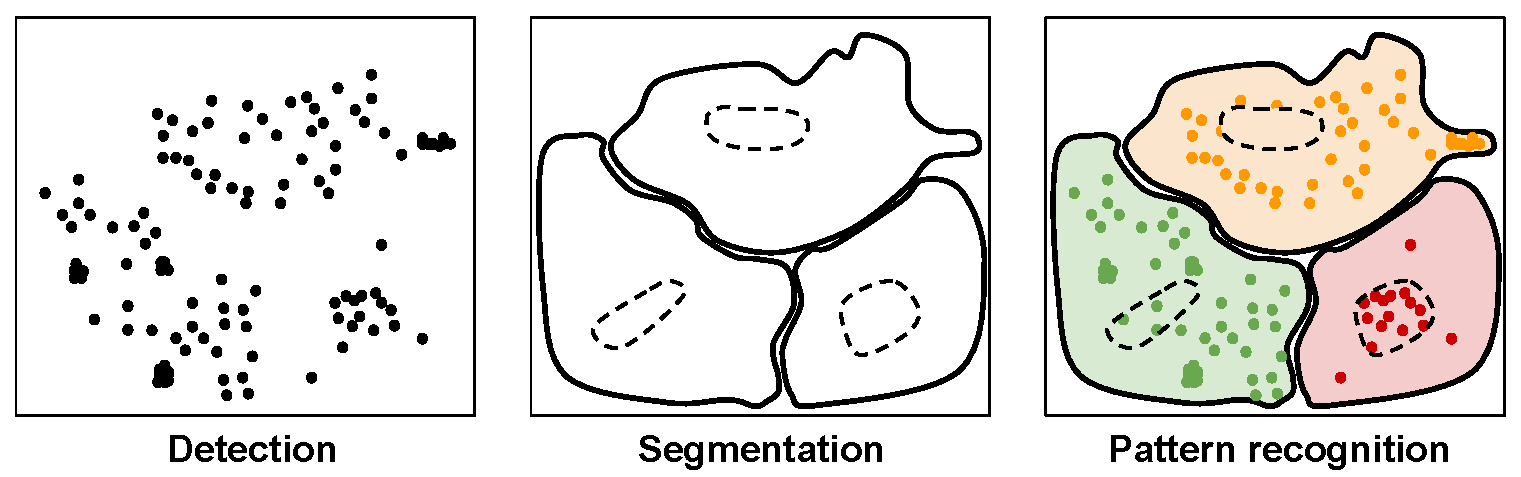
\includegraphics[width=\textwidth]{figures/chapter1/schema_pipeline}
    \caption[Computational pipeline for a smFISH study]{Computational pipeline I use as reference for a smFISH study}
    \label{fig:pipeline}
\end{figure}

\subsection{Related work}
\label{subsec:related_work_fishquant}

Processing a large-scale \ac{smFISH} study requires both specific methods to analyze \ac{RNA} distribution and more general techniques to read and manipulate images based on robust computer vision algorithms.
A \ac{FISH} analysis pipeline hence has to include several inter-dependent subtasks: an accurate \ac{RNA} detection method, the segmentation of relevant subcellular regions such as the cytoplasm and the nucleus, and preprocessing techniques to prepare the images (such that filtering, denoising or projection algorithms).
The obtained results can then be exploited to compute gene expression levels, by counting \ac{RNA} molecules, or develop localization features, to study non-random \ac{RNA} localization.

Specialized solutions for many of these subtasks exist, like BlobFinder~\cite{ALLALOU200958} for spot detection, but using them requires the end-user to assemble a complex analysis workflow, often across different programming languages.
This can be a daunting task, especially for wet-lab biologists with no formal training in computer science.

As an alternative, the development of complete analysis workflows can provide a modular and extensible pipeline for the analysis of \ac{RNA} abundance and localization.
As an example, the Pelkmans Lab published several papers illustrating the need for such complete and robust pipelines.
In~\cite{battich_image-based_2013, stoeger_computer_2015}, the authors develop a modular analysis pipeline permitting to analyze subcellular \ac{RNA} localization from their high-content screen.
The latter paper is a detailed protocol, that permits new users to perform their analysis quickly by providing a detailed description of the implemented approaches.
Further, the advantage of their modular approach, is that additional analysis tasks can be integrated to study related biological questions.
In latter work~\cite{battich_control_2015}, they reused parts of this pipeline to infer \ac{RNA} abundance per cell, and completed this analysis with morphological and phenotypic analysis to explain the observed heterogeneity in \ac{RNA} abundance.

These examples can provide several guidelines for future developments.
First, it is preferable to have a modular framework addressing every step in the \ac{smFISH} analysis pipeline, to facilitate usage.
Second, there is a balance to find between the scope of a framework, its flexibility, its scalability and the amount of user input required.
Lastly, to increase usability of a flexible framework, the analysis steps should be kept modular and be clearly explained.

While several tools exist for each stage illustrated in Figure~\ref{fig:pipeline}, there was - to our knowledge - no tool available that permits performing the entire analysis in one framework.
A complete analysis pipeline has then to be built by mixing these tools and requires some in-house developments, which can be daunting for non-specialists and may provide solutions that are unstable and difficult to scale.
For the segmentation, deep learning has become the method of choice with dramatic improvements in segmentation accuracy as compared to traditional methods.
Spot detection can be performed with different Python or Matlab packages.
However, assigning spot counts to segmentation results and the subsequent analysis of \ac{RNA} levels and RNA localization require custom-written code~\cite{stoeger_computer_2015, samacoits_computational_2018}.
General image analysis tools, such as CellProfiler~\cite{mcquin_cellprofiler_2018}, CellCognition~\cite{held_cellcognition_2010} or Trackmate~\cite{ershov_trackmate_2022}, permit us to establish an analysis framework daisy-chaining some of these analysis steps, but do not permit us to perform the entire analysis.
Steps are missing, usually the ones focused on the \ac{RNA} distribution and localization features computation.

A first attempt to build a software self-sufficient for a \ac{smFISH} analysis was the Matlab version of FISH-quant~\cite{mueller_fish-quant_2013}.
Coupled with a flexible \ac{smiFISH} approach~\cite{tsanov_smifish_2016}, FISH-quant progressively integrated detection and segmentation solutions, in addition to dedicated localization features~\cite{samacoits_computational_2018}.
Today, a number of approaches specifically dedicated to the analysis of \ac{smFISH} are available or in development.
DypFISH~\cite{savulescu_dypfish_2019,savulescu_interrogating_2021} permits the study of the spatial distribution of \ac{mRNA}s and proteins of micropatterned cells.
They mix tools implemented in Python and Icy~\cite{de_chaumont_icy_2012}.
Recently, Bento~\cite{mah_bento_2022} was released to process \ac{SeqFISH}+ and \ac{MERFISH} images, explore and compute spatial features like FISH-quant, with a single-molecule accuracy.
Lastly, StarFISH~\cite{perkel_starfish_2019} is an ongoing software development mainly aiming at solving problems related to multiplex \ac{smFISH} data for application in spatial transcriptomics.
They made a significant effort to be able to read and process images generated by any \ac{FISH} method.

\section{A new framework}
\label{sec:fqv2}

While an impressive range of computational methods already exists, a unified framework dedicated to \ac{smFISH} experiments was lacking.
This prevents users, especially non-specialist, from performing an accurate and large-scale analysis.
To address this, I designed a Python-based version of FISH-quant to fulfill the above-described requirements in a flexible and efficient way~\cite{Imbert_fq_2022}.
Contrary to the first version of FISH-quant in Matlab, I address and improve on each of the specifications mentioned in section~\ref{subsec:pipeline_stages}.
The switch to Python allows me to develop a flexible, free and fully open-source software.
FISH-quant v2 enjoys a better integration to other open source tools and frameworks, from data analysis to web-based user interaction.
Importantly, FISH-quant v2 facilitates the use of machine learning or deep learning algorithms with the import of dedicated packages, such as scikit-learn~\cite{scikit-learn} or TensorFlow~\cite{tensorflow_2015}.
I also improve the scalability and the modularity of the package: the software has now been applied to several High Content Screening projects~\cite{CHOUAIB_2020,safieddine_choreography_2021,pichon_kinesin_2021}.
Lastly, by using ImJoy~\cite{ouyang_imjoy_2019}, a recently developed data analysis framework, we provide browser-based \ac{GUI} for both launching image analysis and downstream analysis of the results, and the computation can be performed locally or seamlessly scale to powerful remote computing servers.

In this section, I will describe the overall organisation of FISH-quant v2 and the architecture of its main components: \emph{bigfish}, \emph{simfish} and the ImJoy plugins.

\subsection{Scalability and modularity}
\label{subsec:framework}

\begin{figure}[]
    \centering
    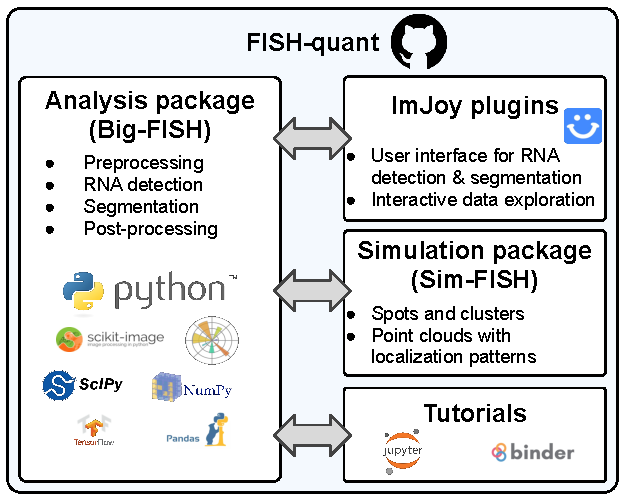
\includegraphics[width=0.8\textwidth]{figures/chapter1/schema_fishquant}
    \caption[Overview of FISH-quant]{Overview of FISH-quant.
	The software is hosted on GitHub and consists of several interconnected repositories.
	The Python core package \emph{bigfish} contains the entire analysis code, which is used by the ImJoy GUIs, the tutorial repository and a simulation package \emph{simfish}}
    \label{fig:fishquant}
\end{figure}

FISH-quant v2 is entirely open-source and hosted on GitHub under the FISH-quant organization\footnote{\url{https://github.com/fish-quant}}.
Using a GitHub organization allowed me to provide dedicated repositories with well defined and dedicated scope (see Figure~\ref{fig:fishquant}).
Further, it gives the flexibility for future extension where new projects can be integrated as new, independent repositories, without affecting and complexifying the already existing code.
The user can choose the adequate code for the analysis needs, without the overhead of installing unnecessary packages.
This GitHub organization is organized in several resources with dedicated repositories and documentation.

First, I implemented a Python package (\emph{bigfish}) providing the core code for performing scalable computation and analysis.
Second, I provide detailed interactive examples with test data for each analysis step that are available in Jupyter notebooks.
These examples can also be run directly on Binder~\cite{Jupyter2018Binder2}, a free and reproducible Jupyter notebook service, without local installation.
Third, a Python package (\emph{simfish}) allows the simulation of different subcellular \ac{RNA} localization patterns.
Fourth, ImJoy plugins~\cite{ouyang_imjoy_2019} provide a \ac{GUI} for the most commonly used workflows, and an interactive tutorial that can also run directly without local installation.
Lastly, a landing page\footnote{\url{https://fish-quant.github.io/}} centralizes implemented tools and directs new users to the most relevant resource for their analysis needs.

Dependencies for the Python packages are limited to standard Python scientific libraries: scientific computing (numpy~\cite{2020NumPy}, SciPy~\cite{2020SciPy}), data wrangling (pandas~\cite{mckinney_pandas_2010}), image analysis (scikit-image~\cite{walt_scikit-image_2014}), visualization (matplotlib~\cite{hunter_matplotlib_2007}), parallel computing (joblib\footnote{\url{https://github.com/joblib/joblib}})and machine learning (scikit-learn~\cite{scikit-learn}, TensorFlow~\cite{tensorflow_2015}).
The GitHub repositories are using continuous integration providing increased robustness of the released code, through unitary testing, version control and automatically generated up-to-date documentation.
Finally, packages are hosted under a BSD 3-Clause License.

\subsection{Big-FISH}
\label{subsec:bigfish}

\subsubsection{\emph{pip install big-fish}}

We chose to implement the core analysis package \emph{bigfish} in Python.
Compared to MATLAB, Python allows the development of a free and fully open-source software.
It also provides access to established libraries for data and image analysis, in addition to the most popular deep learning frameworks.
Lastly, Python packages can be interfaced with other tools and frameworks, from data analysis to web design, to provide interactive tools for user interaction and data inspection.

As shown in Figure~\ref{fig:bigfish}, \emph{bigfish} includes several independent subpackages for the different steps in a \ac{smFISH} analysis workflow: preprocessing, detection, segmentation, and analysis.
I designed each subpackage with clearly defined input and output data formats, which are automatically checked.
Each of these packages can be used independently in a modular fashion.
Users can thus create a customized analysis workflow, starting from preprocessing of images to statistical interpretation of results.
These workflows can be implemented in Python and Bash scripts and run both on local and remote computational resources.
The modular design also permits the easy integration of external methods, for instance, a new segmentation method can be combined with this spot detection algorithm.

More specifically, the Python code used in \emph{bigfish} package is organized in 7 subpackages performing dedicated steps:
\begin{itemize}
	\setlength\itemsep{0.1em}
	\item \emph{bigfish.stack} - I/O operations and images preprocessing
	\item \emph{bigfish.detection} - \ac{mRNA} spot detection
	\item \emph{bigfish.segmentation} - nucleus and cell segmentation
	\item \emph{bigfish.multistack} - post-processing and analysis of results from different channels, such as the merging of \ac{RNA} detections and segmentation masks or colocalization analysis
	\item \emph{bigfish.classification} - localization feature computation
	\item \emph{bigfish.plot} - visual reports of the obtained results
	\item \emph{bigfish.deep\_learning} - deep learning algorithms and pretrained models for segmentation or point cloud analysis
\end{itemize}

In this chapter, I provide only an overview of these subpackages.
More details can be found in subsequent chapters where I discuss particular algorithms that I have designed or implemented, or both.
I would also like to refer interested readers to the package documentation\footnote{\url{https://big-fish.readthedocs.io/en/stable/}} or the GitHub repository\footnote{\url{https://github.com/fish-quant/big-fish}}.
Dedicated notebook tutorials are also available\footnote{\url{https://github.com/fish-quant/big-fish-examples}}.
They can be run directly in the browser with Binder~\cite{Jupyter2018Binder2} and provided sample data, and thus allows new users to immediately test the package.

\begin{figure}[]
    \centering
    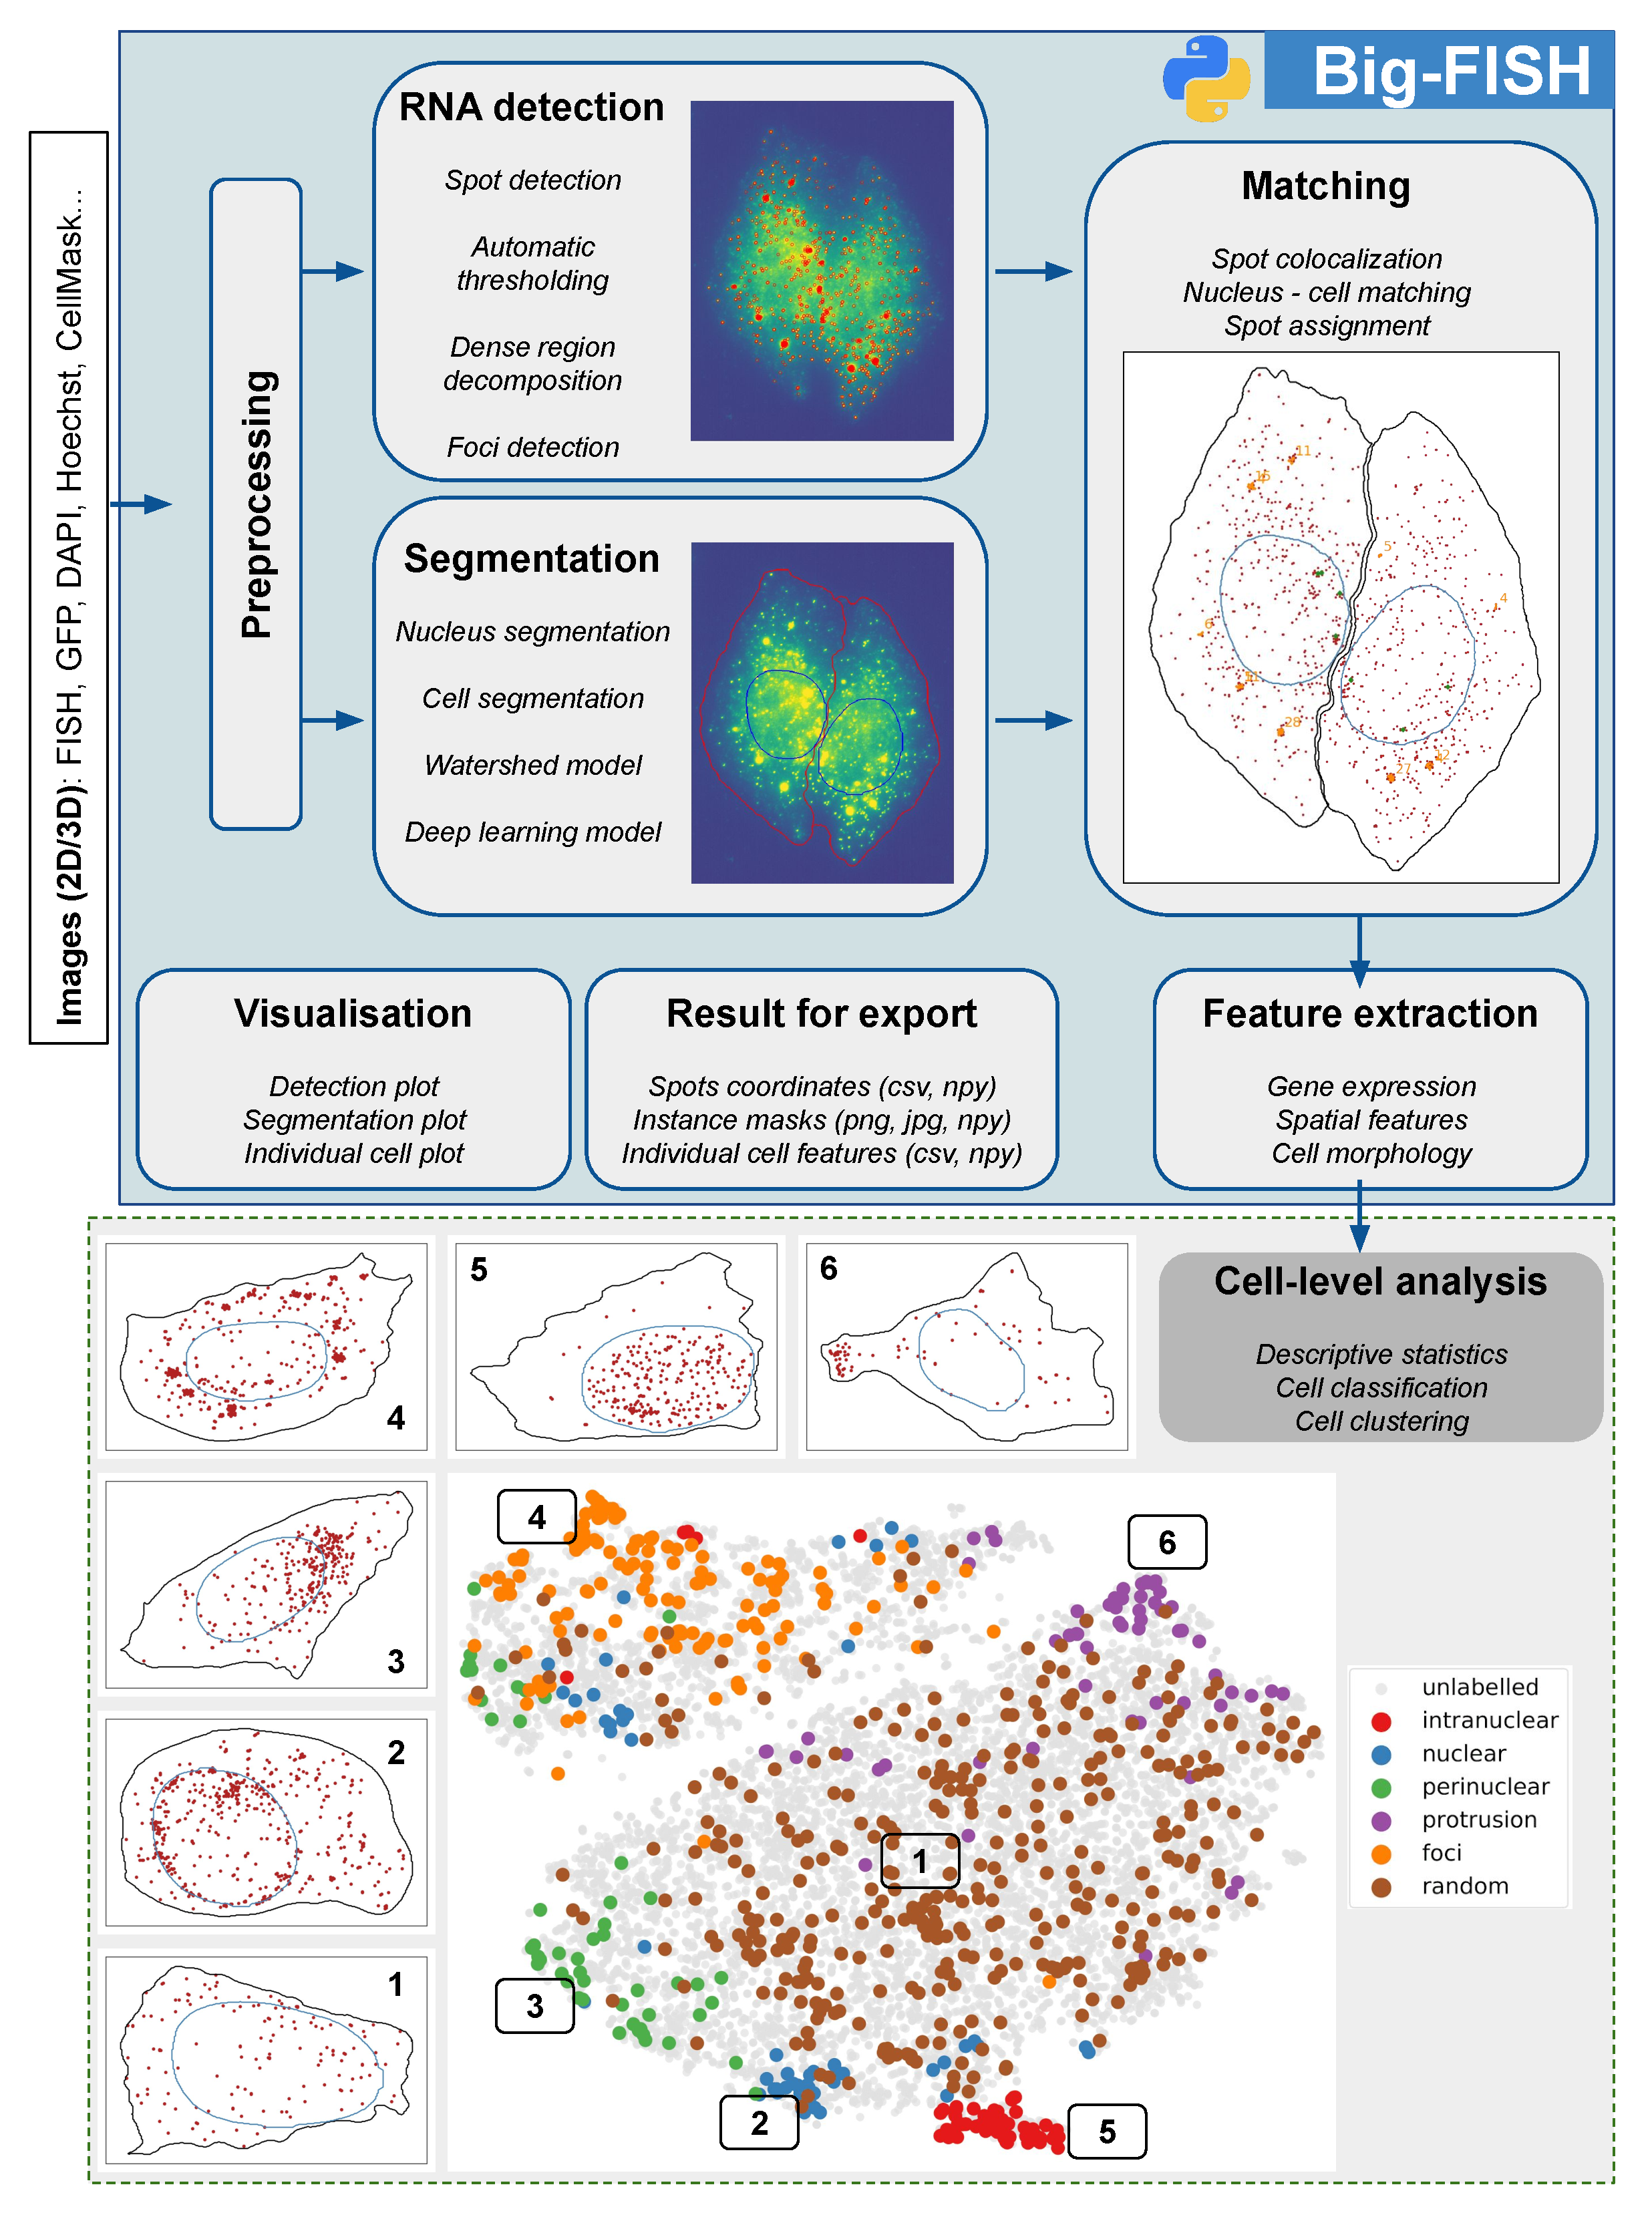
\includegraphics[width=0.95\textwidth]{figures/chapter1/schema_bigfish_full}
    \caption[Overview of \emph{bigfish}]{Overview of \emph{bigfish}.
	(\textit{Upper part}) Main modules illustrated with a typical analysis workflow.
	Shown are also the inputs and outputs that are created at the different steps.
	(\textit{Lower part}) Not directly included in \emph{bigfish}.
	As a final result, each cell is described with a set of features reflecting RNA abundance and localization.
	These features can then be used to perform analysis on the cell population.
	Results from~\cite{CHOUAIB_2020} are illustrated as example (see chapter~\ref{ch:chapter5} for more details).
	The t-SNE plot projects 15 localization features for smFISH experiments against 27 different genes.
	Each dot is one cell.
	The color-coded dots are manual annotations of six different localization patterns.
	Images are examples of individual cells displaying a typical localization pattern of this region of the t-SNE plot}
    \label{fig:bigfish}
\end{figure}

\subsubsection{Building blocks for a full analysis pipeline}

The package \emph{bigfish} aims at addressing the main challenges in \ac{smFISH} analysis.

First, for image handling and preprocessing, I implemented a number of different utility functions to read, write, normalize, cast, filter, and project images.
Different image file formats are natively supported and both 2D and 3D images can be processed.
These methods are gathered in \textbf{bigfish.stack}.

Second, the detection subpackage (\textbf{bigfish.detection}) provides methods required to detect spots in 2D or 3D images.
An important aspect of my implementation is its ability to detect spots without setting any pixel intensity threshold.
I propose a method to automatically infer this threshold from the image.
Such automatization overcomes human intervention and allows scaling to large data sets, such that the subpackage can process thousands of images.
While initially designed to detect individual \ac{mRNA}s, this subpackage permits the detection of larger spot-like structures like P-bodies or centrosomes (see applications in chapter~\ref{ch:chapter5} for more details).
Furthermore, I provide a fitting method to localize spots with a subpixel accuracy, a colocalization algorithm and cluster detection.
Strong local accumulation of \ac{RNA}s can lead to an underdetection since such accumulations are counted as single \ac{RNA}s.
For such cases, I also provide tools to decompose these dense regions and estimate the right number of spots.
The chapter~\ref{ch:chapter2} gives a comprehensive description of the implemented detection methods.

Third, the segmentation subpackage (\textbf{bigfish.segmentation}) contains several algorithms and utility functions for segmentation and post-processing.
It provides a simple deep-learning-based approach to segment cells and nuclei, but also traditional methods such as thresholding or watershed.
Furthermore, different post-processing tools are available to refine and clean the segmentation result, such as boundary smoothing, removal of small objects or filling of small holes.
These algorithms are presented with more details in the chapter~\ref{ch:chapter3}.

Forth, detected \ac{RNA} point clouds need to be matched to their cellular or subcellular environment.
For this, the subpackage \textbf{bigfish.multistack} enables to combine detection and segmentation results, obtained from different input channels.
It permits the analysis of \ac{RNA} abundance and distribution at the single-cell level.
Detected spots can be assigned to a specific region of interest, for instance, a cell or a nucleus.
Using the same method, \ac{RNA} clusters can be assigned to a nucleus and thus be considered as transcription sites.
\ac{RNA} expression levels are computed within this subpackage, as this is usually the minimum information that is extracted from a spatial transcriptomics study.

Finally, the subpackage \textbf{bigfish.classification} computes features at the single cell level from the spot positions and the coordinates of cellular landmarks.
These features allow a statistical description of the cell population or can feed a classification model allowing for the discrimination of individual cells according to their RNA localization patterns.
More information about the cell matching step and the feature engineering are presented in chapter~\ref{ch:chapter4}.

In \emph{bigfish}, I also provide a subpackage (\textbf{bigfish.plot}) to visualize the results of each intermediate step in the analysis workflow and thus provide valuable visual quality control.
A last subpackage (\textbf{bigfish.deep\_learning}) gathers the utility functions and model architectures to run deep learning solutions.
The use of such techniques implies more complex dependencies in the back-end like TensorFlow~\cite{tensorflow_2015}.
By isolating pieces of code related to deep learning, I make the import of these frameworks optional for the user.
Indeed, the majority of the methods provided by \emph{bigfish} does not require artificial neural networks.

\subsection{Sim-FISH}
\label{subsec:simfish}

The Python package \emph{simfish} is dedicated to the simulation of \ac{FISH} images.
These simulations come in two flavors: simulation of \ac{smFISH} image simulation and simulation of point cloud coordinates with a specific localization patterns.

Spots or clusters of spots with various intensities and shapes can be simulated, in 2D or 3D, optionally with subpixel accuracy.
Different parameters, such as the number of spots, the size of the clusters and even the background noise level or randomness in the image can be controlled by the user.
These simulated images can be used to validate spot or cluster detection methods, for instance to evaluate the impact of varying noise levels.
I refer to the chapter~\ref{ch:chapter2} for the details about the generation of these images.

The simulated point clouds are used to build a large dataset with different \ac{RNA} localization patterns.
They can be used for benchmarking and ultimately for the training of neural networks for classification of localization patterns.
The output of the simulation is not an image, but a list of 3D \ac{RNA} coordinates as well as the 2D cell and nuclear boundaries.
The localization pattern can be chosen among 9 predefined patterns, and the strength of the pattern (and thus the difficulty of recognizing the pattern) can be controlled by one parameter.
Chapter~\ref{ch:chapter4} provides a thorough description of the simulations.

More generally, such simulations can be helpful to validate, calibrate or pre-train algorithms.
This is particularly true when we deal with experimental data difficult to generate or annotate.
Lastly, online information about the simulation package are available in the documentation\footnote{\url{https://sim-fish.readthedocs.io/en/stable/}} or in the GitHub repository\footnote{\url{https://github.com/fish-quant/sim-fish}}.

\subsection{ImJoy}
\label{subsec:imjoy}

\begin{figure}[]
    \centering
    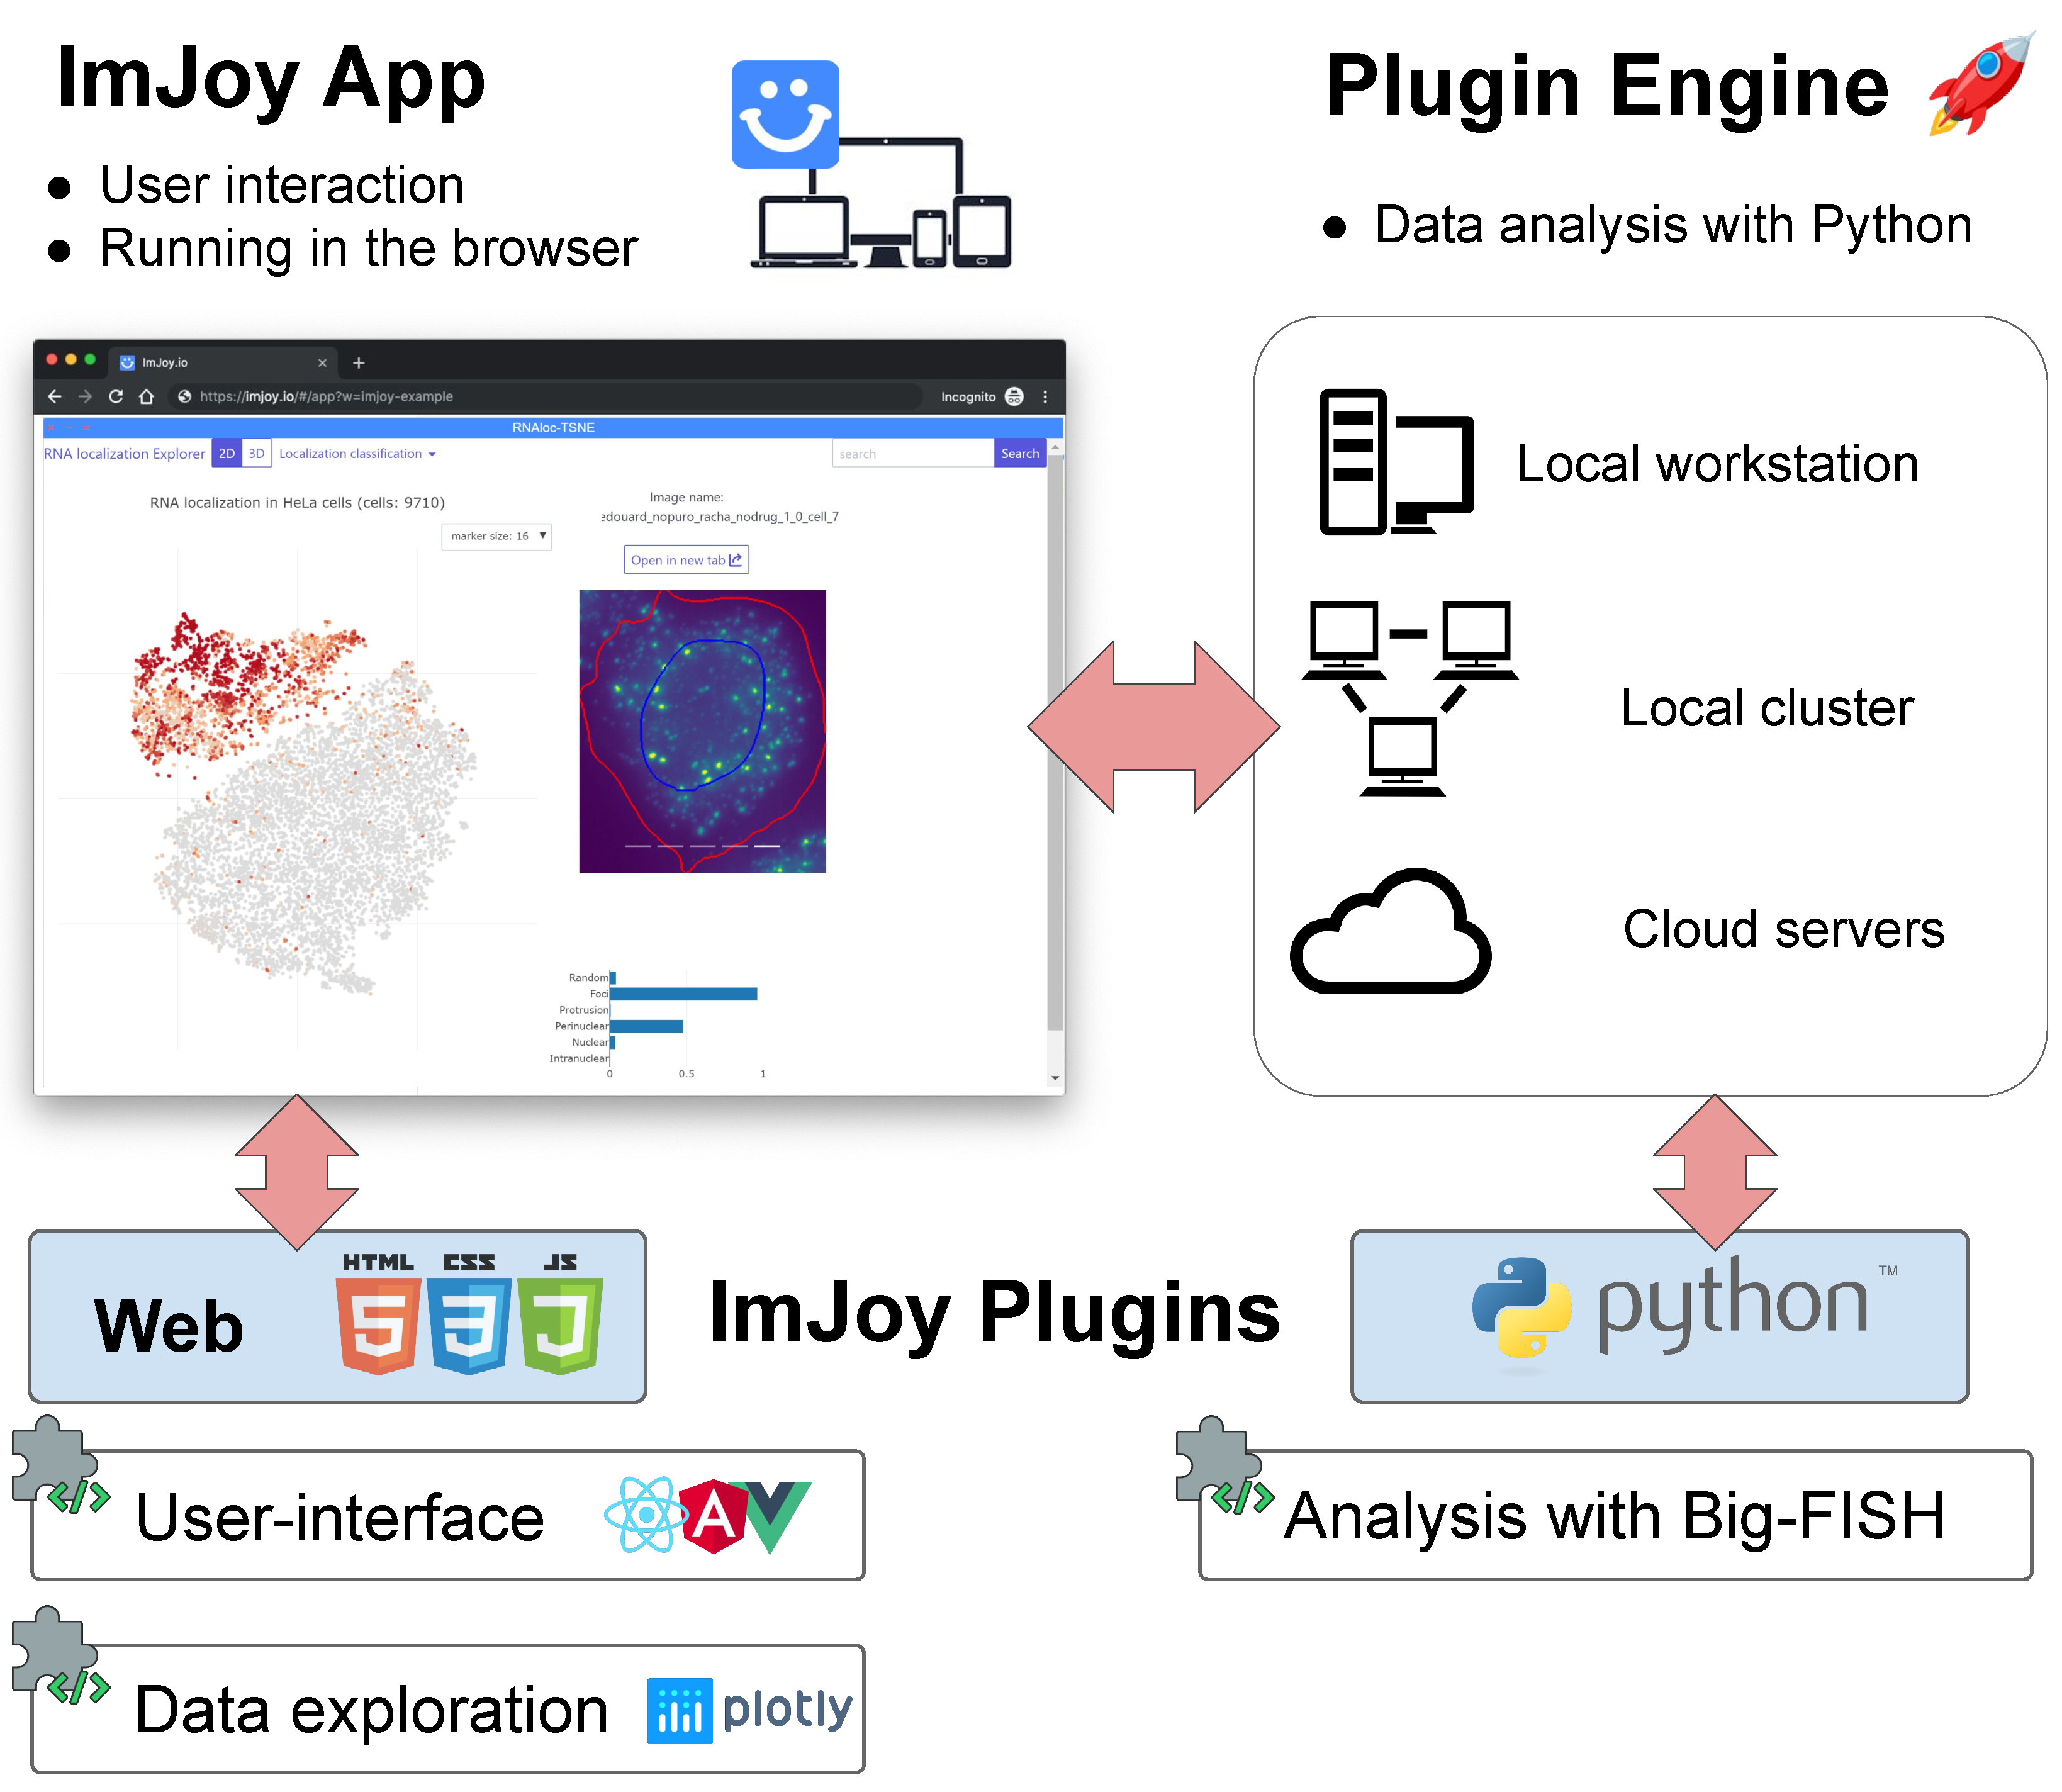
\includegraphics[width=0.8\textwidth]{figures/chapter1/schema_imjoy}
    \caption[Overview of ImJoy]{Overview of ImJoy.
	(\textit{Top}) ImJoy's core is a Progressive Web App whose functionalities are provided by plugins run directly in the browser or on a plugin engine (local or remote).
	Plugin engines support the scientific Python ecosystem and dependency management is handled with Conda.
	(\textit{Bottom}) Browser plugins are implemented with HTML, CSS or JavaScript.
	They allow user interaction, data visualization and computation in the browser.
	Heavier computations can be run from a Python plugin engine before being displayed in the web app}
    \label{fig:imjoy}
\end{figure}

The \emph{bigfish} package provides flexibility and scalability since its components can be adapted to the specific analysis needs of a given project.
However, it requires at least a minimum knowledge of Python to establish a complete workflow by using the provided tutorials.
We thus implemented several plugins with a \ac{GUI} for ImJoy ~\cite{ouyang_imjoy_2019}.
A general organization of ImJoy is illustrated in Figure~\ref{fig:imjoy}.
It provides simpler access for users with no computational background and no programming skills.
These plugins provide the most commonly used analysis workflow, as determined from the usage of the Matlab version of FISH-quant~\cite{mueller_fish-quant_2013}, and will thus be suited for a large number of use cases.
It mostly includes segmentation and detection tools.

First, we implemented a plugin to perform segmentation on top of CellPose model~\cite{stringer_cellpose_2021}.
Thanks to the modular design, this model can be easily exchanged if more performant methods are available in the future.
A documentation is available online to launch and run the plugin\footnote{\url{https://fq-segmentation.readthedocs.io/en/latest/}}.

We also implemented a detection plugin based on \emph{bigfish} modules.
Both isolated and clustered \ac{RNA} can be detected and detection results can be inspected with the Kaibu image viewer plugin in ImJoy.
While \emph{bigfish} is developed to be scalable without the need to fine tune parameters, different detection settings can be interactively investigated through the \ac{GUI}.
Batch processing of entire folders is also possible.
Lastly, detection results can be assigned to segmented cells and nuclei if segmentation masks are available.
An online documentation is available for this plugin\footnote{\url{https://fq-imjoy.readthedocs.io/en/latest/}}, and also an interactive demo\footnote{\url{https://fish-quant.github.io/fq-interactive-docs/\#/fq-imjoy}}.
This demo can be run directly in the browser without any local installation.

Using ImJoy provides several advantages compared to a stand-alone \ac{GUI}.
Due to its distributed design that separates \ac{GUI} from computation plugins, it natively supports user-friendly remote computing which allows access to massive data storage and powerful computation resources including GPUs.
ImJoy is a Progressive Web App where the user interface plugin is implemented with front-end languages like HTML, CSS or JavaScript.
It then transparently calls the \emph{bigfish} methods running on a Python plugin engine (for example a Jupyter notebook server) to perform the actual \ac{smFISH} analysis task.
While this plugin can run on a local workstation, it can be executed on a computational cluster or even in the cloud or seamlessly switching between them.
For example in our demo version, the engine is running on Binder~\cite{Jupyter2018Binder2}.
Once the plugin engine is installed on the remote resource, the end-user can connect with ImJoy and will be confronted with the same interface (the browser plugin), independently of where the analysis is actually performed.
Interestingly, this front-end interface can also be opened with mobile devices.
ImJoy plugins implemented in JavaScript not only provide modern and reactive user interfaces, but also profit from the extensive JavaScript resources in terms of data visualization and interactivity.
Such interactivity is becoming increasingly important, especially when large and complex data sets are analyzed where static plots are too limited.
As a case example, we provide an interactive t-SNE plot\footnote{\url{https://fish-quant.github.io/fq-interactive-docs/\#/rnaloc-tsne}} for the data analyzed in~\cite{CHOUAIB_2020} and detailed in chapter~\ref{ch:chapter5}.
This plugin can be run without local installation and enables the user to explore and interact with these complex data.

\section{Conclusion}
\label{sec:conclusion}

In this chapter I present the second version of FISH-quant, a user-friendly Python based framework for the complete analysis of \ac{smFISH} images.
It is built around \emph{bigfish}, a core-analysis package, implemented following rigorous software development guidelines, with detailed interactive documentation and tutorials.
This package consists of several interchangeable modules whose organization matches key steps in \ac{smFISH} image analysis: preprocessing, \ac{RNA} detection, cell segmentation and analysis.
Its modularity permits the creation of flexible workflows ranging from the analysis of small data sets with the help of a \ac{GUI} to custom-tailored investigation of large-scale screens requiring computational clusters.
Indeed, I also provide user interfaces in ImJoy accessible to biologists without programming skills, which can be used locally or scaled to larger remote computational resources, and displayed in the browser.
A last package, \emph{simfish}, allows the simulation of \ac{smFISH} images with non random \ac{RNA} localization patterns.
These simulations can be used to develop and evaluate analysis pipelines.
Lastly, the use of Python scientific ecosystem, as well as strict version control and minimal dependencies, facilitate installation, maintenance and integration with other analysis or visualization frameworks.
All dependencies, as well as FISH-quant v2, are open-source, thus can be used free of charge.

In the chapters~\ref{ch:chapter2},~\ref{ch:chapter3} and~\ref{ch:chapter4}, I detail the different functions available in FISH-quant.
Throughout the manuscripts, I thus include several snippets with the few lines of code related to the described methods. %
%%!TEX root = ../main.tex

\graphicspath{{./figures/chapter2/}}

\chapter{Single RNA Detection}
\label{ch:chapter2}

\minitoc
\newpage

In \ac{smFISH} images, \ac{RNA} molecules appear as diffraction limited spots
For this reason, the detection of individual \ac{RNA} molecules boils down to spot detection, a problem that has been largely addressed by different scientific communities.

After a review of different techniques for spot detection, I will discuss shortcomings of existing methods when applied to High Content Screening by \ac{FISH} and describe the solution I have developed and implemented in \mbox{\emph{bigfish.detection}}.
Finally I evaluate robustness and accuracy of this implementation by applying the algorithm on simulated data under different noise conditions.
These results are published in the paper~\cite{Imbert_fq_2022}:

\begin{center}
	\color{green}
	A. Imbert, W. Ouyang et al. (2022), \textit{FISH-quant v2: a scalable and modular tool for smFISH image analysis}, RNA, pp. $\operatorname{786--795}$, iSSN: $\operatorname{1355--8382, 1469--9001}$.
\end{center}

\section{Spot detection as a signal processing problem}
\label{sec:detection_introduction}

This introductory section is devoted to a description of the spot detection problem, and a review of solution proposed in the literature.  

\subsection{Problem description}
\label{subsec:detection}

From an image with identifiable point sources, the aim of spot detection is to extract an array of spatial coordinates corresponding to the spot centers.
This task is performed in two or three dimensions, depending of the input image.\\

\noindent
Detecting an object as small as an \ac{RNA} molecule faces several challenges:
\begin{enumerate}
	\setlength\itemsep{0.1em}
	\item The optical system does not capture the original light signal emitted by the fluorescence probes, but its convolution with a \ac{PSF}.
	In this thesis, I will assume that the \ac{PSF} can be approximately described by a Gaussian in 2 or 3 dimensions.
	Such simplification is reasonable for a detection with pixel accuracy, given a good \ac{SNR}.
	\item As we can observe in Figure~\ref{fig:detection_results}, a \ac{smFISH} image often presents a background fluorescence, stemming from reporter molecules that are not specifically binding to target \ac{RNA} and which are uniformly distributed in the cytoplasm.
	In 2D images, we thus observe that the background signal is roughly proportional to the local height of the cell.
	\item We can observe noise that actually resembles the signal we wish to detect, but at lower intensity.
	\item Both signal and noise can be highly heterogeneous and vary between images and between cells inside the same image.
	\item Depending on the density and the localization patterns, \ac{RNA} molecules might be in close proximity.
	They might form clusters, for which no individual spots are distinguishable.
	In this case, the detection of individual \ac{RNA} molecules might not be possible without simplifying assumptions.
\end{enumerate}

In the context of a high content screening, a large number of images are acquired, with various biological samples or conditions.
For this reason, heterogeneity regarding pixel intensity and spot distributions represent a serious problem.
At the same time, the number of images is such that we cannot reasonably manually adapt parameters for individual images (let alone individual cells).
It thus requires a robust approach to tackle this problem and extract accurate coordinates of the spot positions.

\begin{figure}[]
    \centering
    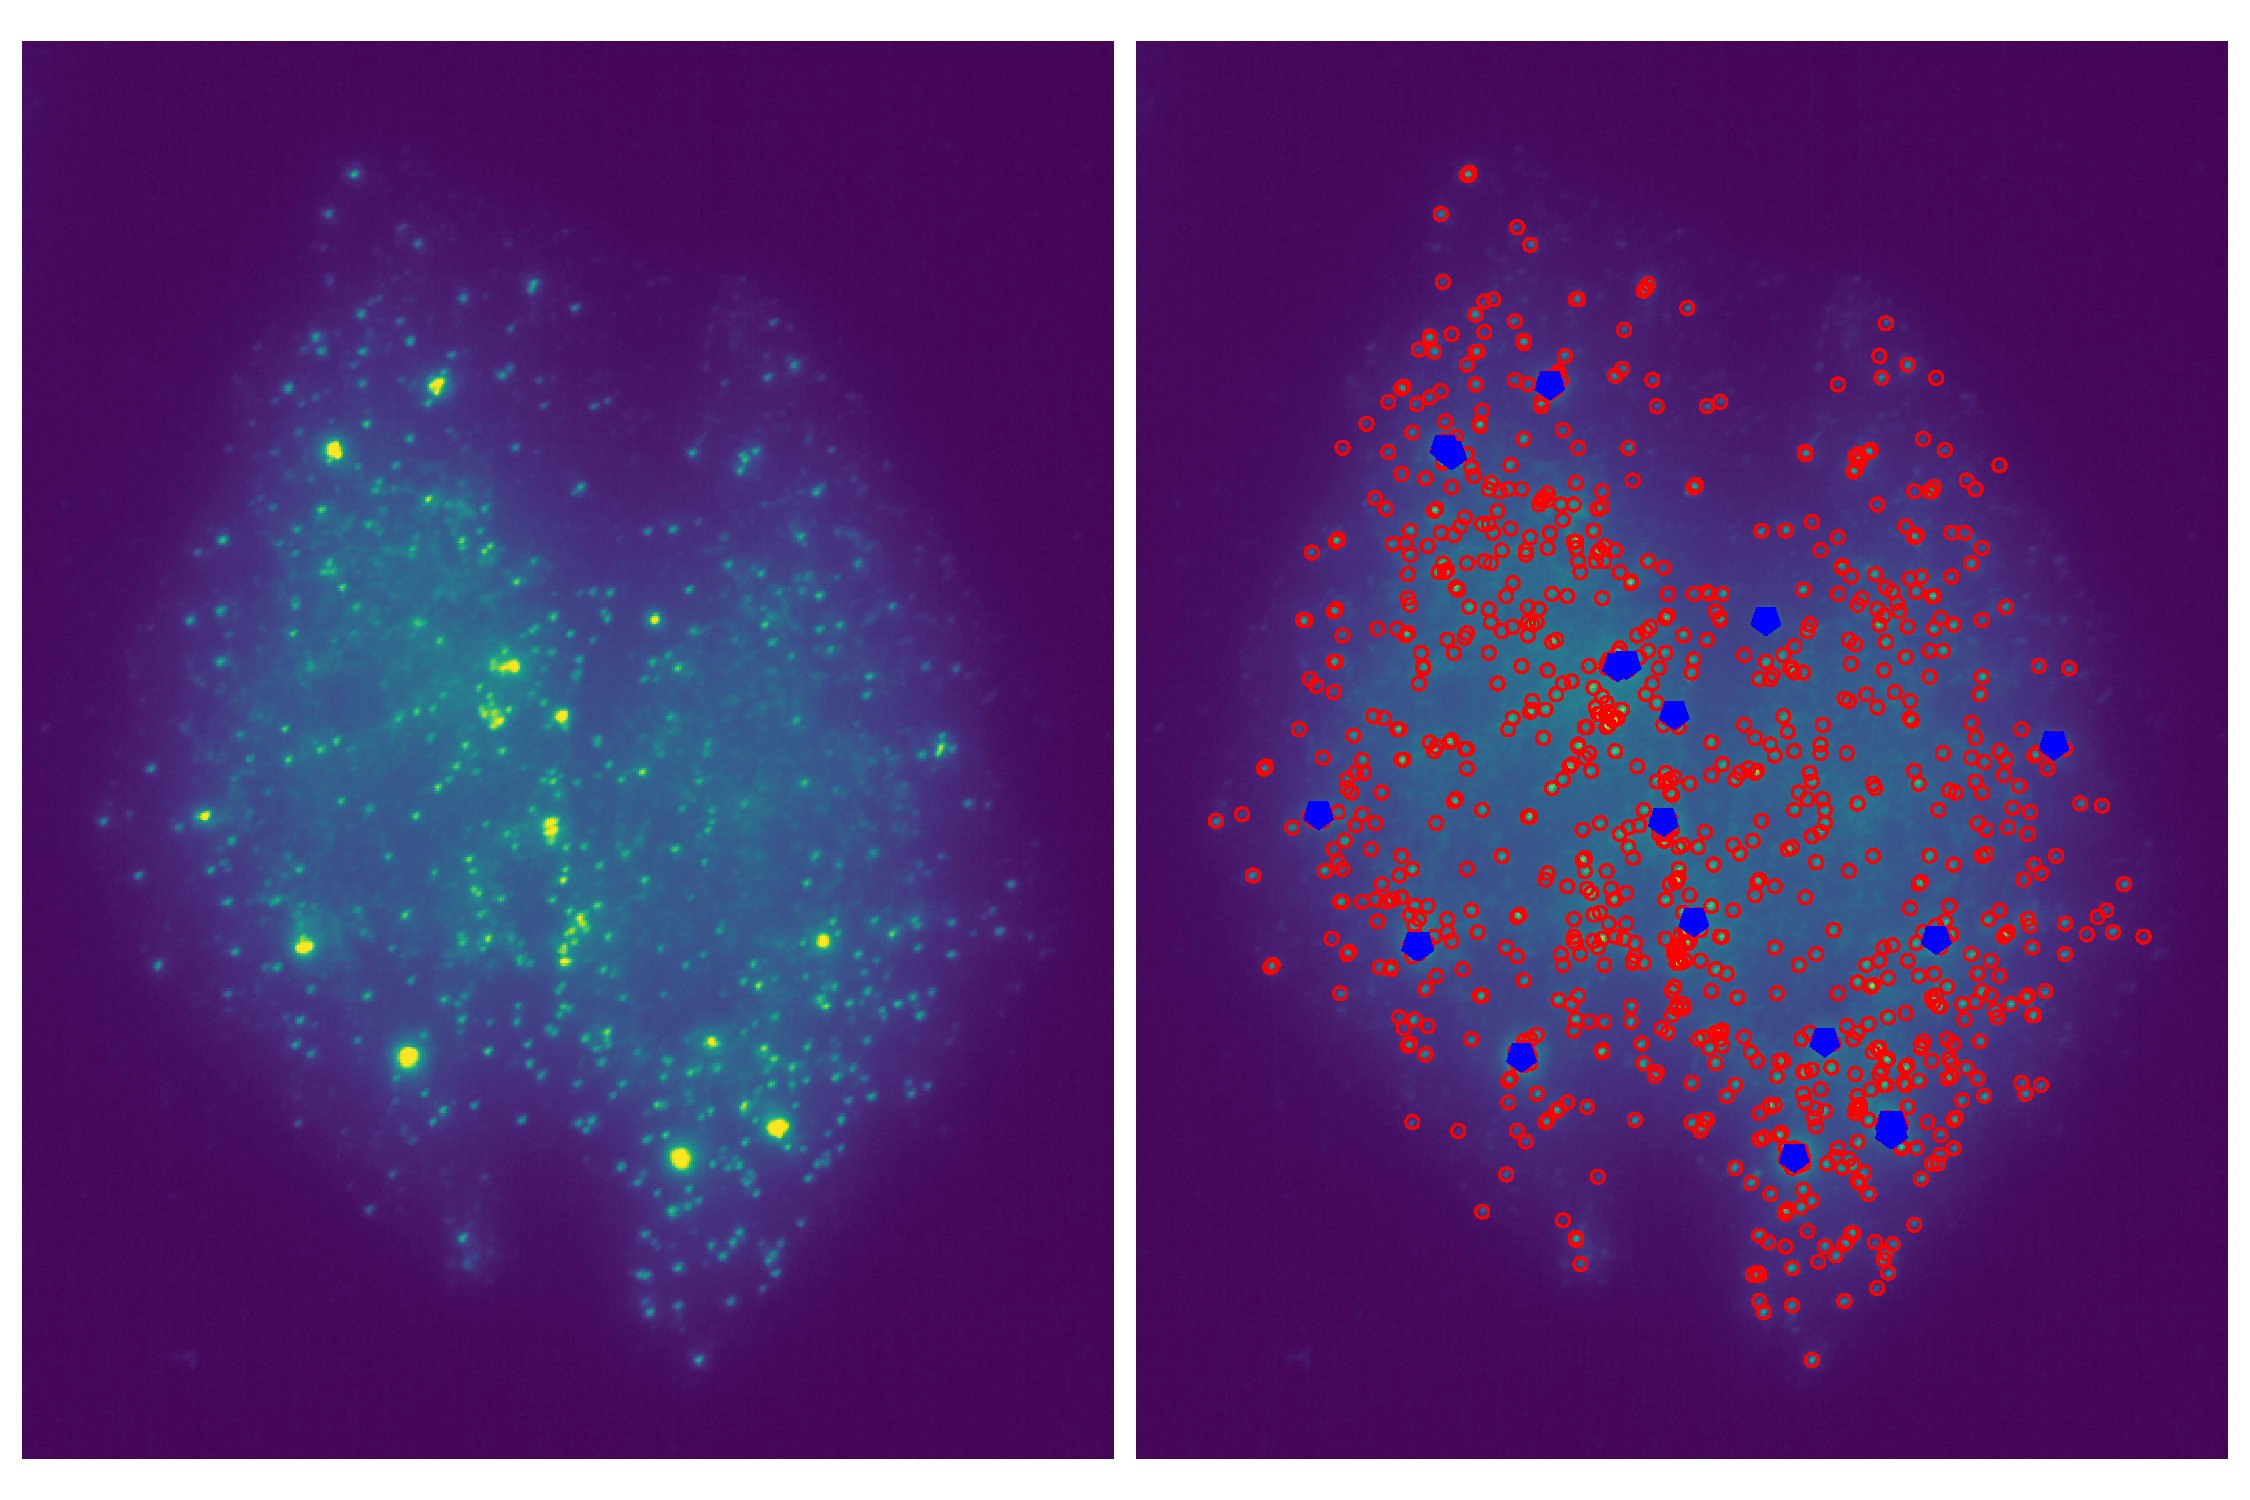
\includegraphics[width=1\textwidth]{figures/chapter2/cluster_detection_results}
	\caption[Example of spot detection results]{Detection results.
	(\textit{Left}) Original smFISH image.
	(\textit{Right}) Spots in \textit{red} and clusters in \textit{blue}, detected with \emph{bigfish.detection}}
    \label{fig:detection_results}
\end{figure}

\subsection{Related work}
\label{subsec:detection_related_work}

\subsubsection{Traditional approaches based on filtering and thresholding}

Spot detection, especially for fluorescent images, has been addressed by the scientific community through different approaches.
Classical approaches usually rely on filtering approaches that specifically enhance spot-like features, and binarization by thresholding or maxima detection.

\paragraph{Methods}

Most spot detection methods can be decomposed into 3 steps: reduction of noise, signal enhancement and signal thresholding~\cite{smal_quantitative_2010}.

A popular method to reduce noise while enhancing spot-like structures is the convolution with a Gaussian filter.
Filtering enhances the structures that resemble the filter itself, while attenuating high-frequency noise.
Under the assumption of a Gaussian \ac{PSF}, a Gaussian filter is supposed to be particularly efficient.
Alternative methods for noise reduction and signal enhancement include wavelet-based filtering, where the signal is decomposed with the Wavelet transform and non-significant Wavelet coefficients are discarded~\cite{Olivo-Marin2002}.

Signal enhancement refers to the specific enhancement of spot-like structures.
As the spots we aim at detecting are small with respect to all other structures in the image, a popular strategy is to remove spots by some filter operation $\psi$ and to consider the residue $g - \psi(g)$ for further processing, where $g$ is the prefiltered image from the first step.
Here, $\psi$ might be a Gaussian filter (thus leading to the classical \ac{DoG} filter~\cite{Lindeberg2015}) or a morphological filter, such as the h-dome image~\cite{smal_quantitative_2010}, or diameter openings~\cite{Walter2007}.
An alternative consists in evaluating the second order derivative by calculating the \ac{LoG}.
It can be shown that this approach is closely related to the \ac{DoG} filter~\cite{Lindeberg2015}.

The third step is binarization.
This is usually achieved by either thresholding the enhanced image or identification of local maxima, usually followed by application of additional criteria, such as intensity (which is also a form of thresholding).

These three steps can be complemented by additional post-processing methods to disentangle close spots and refine the positions of the detected spots by \ac{PSF} fitting or exploitation of radial symmetry~\cite{bahry_rs-fish_2021}.
Overall, it can be said that smFISH usually provides high \ac{SNR} images for cell culture, and differences between these detection methods are often marginal~\cite{smal_quantitative_2010}. 

\paragraph{Implementations}

In general, software for \ac{RNA} detection can rely on several spot detection algorithms that are already implemented and available in popular Python packages like \emph{scikit-image}~\cite{walt_scikit-image_2014} or \emph{astropy}~\cite{astropy_2018}.
Astropy community developed an affiliated package \emph{photutils}~\cite{larry_bradley_2020_4044744} with helpful functions for photometry of astronomical sources like \ac{PSF} matching or source detection.
Software tools for \ac{RNA} detection in Python can thus rely on these libraries.

There are also existing dedicated software solutions for the detection of RNAs, implemented in the three ecosystems used in bioimage informatics: Java, Python and MATLAB.
For instance, Icy (implemented in Java), proposes a wavelet-based method for spot detection~\cite{de_chaumont_icy_2012}, the ImageJ/FIJI plugin Trackmate (also implemented in Java) implements a blob detection pipeline with \ac{LoG} filters~\cite{ershov_trackmate_2022}, the recently published RS-FISH~\cite{bahry_rs-fish_2021} proposes \ac{DoG} filters with refined localizations as a FIJI plugin~\cite{schindelin_fiji_2012} (implemented in Java).
The recent Python library \emph{starfish}~\cite{perkel_starfish_2019} wraps existing \emph{scikit-image} functions and the first FISH-quant version~\cite{mueller_fish-quant_2013} (implemented in MATLAB) includes a blob detection pipeline with a \ac{LoG} filter.
This last pipeline is the one we implemented and improved in our work for \emph{bigfish.detection}.

Besides the processing capabilities and the specific implementations, most of the cited solutions also come with a \ac{GUI}, namely Icy, Trackmate, FISH-quant and RS-FISH.
One important aspect of these \ac{GUI}s is to manually adapt algorithmic parameters, in particular the detection threshold.

This last point is a major limitation for us.
The need for parameter tuning is a critical bottleneck for scaling detection.
When we apply an algorithm to thousands of images, with noise and intensity heterogeneity, most parameters need to be set once (or automatically) and not recalibrated between images.
In particular most of the presented methods require a threshold or a size parameter at some point.

\subsubsection{Learning-based methods}

Spot detection has also been addressed by recent deep learning methods.
Deep learning (or more generally computer vision), allows one to perform spot detection without the a-priori definition of filters, models and criteria, and prevent parameter tuning on a cell-by-cell or image-by-image basis at the cost of a training stage, thus implying the establishment of ground-truth data.

A first study~\cite{bouilhol_deepspot_2022} proposes to preprocess images to make spot intensity homogeneous.
A convolutional network (named DeepSpot) is trained to enhance spot signal to the same intensity.
The network has two main components: a \ac{CASO} module followed by a customized ResNet~\cite{He_2016}.
\ac{CASO} mixes standard convolution blocks with strided and atrous (or dilated) convolutions~\cite{Hamaguchi_2018}.
Small objects like spots do not contain enough semantic information to be captured.
Standard convolution blocks (with max pooling) are great to learn semantic information, but at the expense of lower intensity spots and a potential spatial information loss.
One the one hand, replacing the pooling layer with strided convolution compensates the lower intensity.
On the other, the use of atrous convolution increases receptive field and thus improves context information with a minimal spatial information loss.

Another model, DeepBlink~\cite{eichenberger_deepblink_2021}, is based on a U-Net architecture~\cite{Ronneberger_2015} and directly detects spots.
The U-Net component extracts intermediate features.
Then it maps the original image into \emph{grid-cells} (small bounding-boxes) for which model predicts the probability of a spot localization and the potential 2D coordinates.
Size of the \emph{grid-cell} is critical.
With a small size, too many cells might be empty, resulting in an imbalanced dataset for the classification head of the model.
On the opposite, with a larger size, one cell could contain multiple spots (for only one prediction per \emph{grid-cell}).
This process is directly inspired by the detection model YOLO~\cite{Redmon_2016_CVPR}.

\section{Scaling mRNA detection}
\label{sec:method}

We now describe at depth the algorithms currently implemented in \emph{bigfish.detection}.

\subsection{Spot detection}
\label{subsec:spot_detection}

The method we use is directly adapted from the original version of FISH-quant~\cite{mueller_fish-quant_2013} and the blob detection algorithms~\cite{walt_scikit-image_2014}.
Detection is performed in 2D or 3D. Images are filtered in order to increase \ac{SNR}, then each spot is defined as a local maximum above a specific threshold.

\subsubsection{Filtering}

\begin{figure}[]
    \centering
    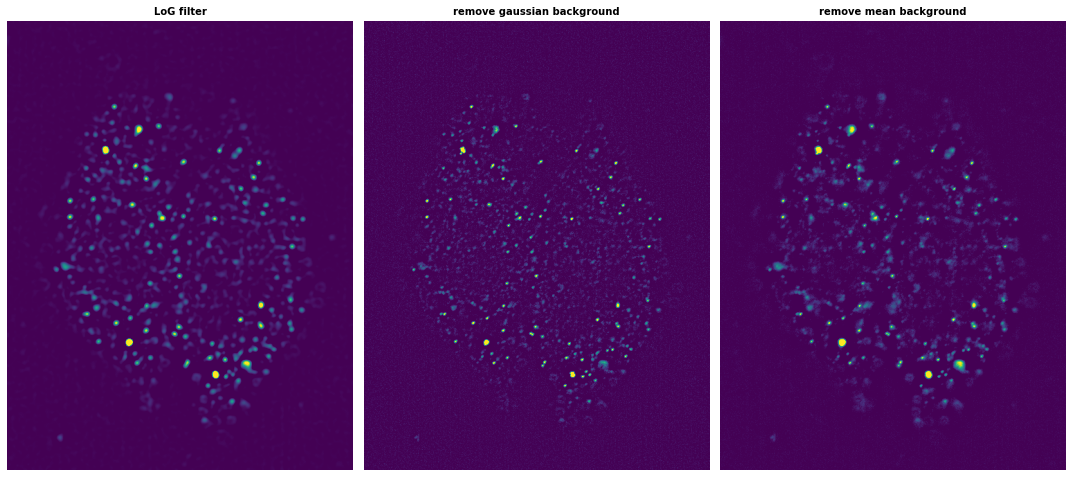
\includegraphics[width=1\textwidth]{figures/chapter2/filter_background}
    \caption[Filtered images with LoG and DoG filters]{Filtered images with LoG filter (\textit{Left}) and DoG filter (\textit{Right})}
    \label{fig:filters_detection}
\end{figure}

We apply a \ac{LoG} filter (Gaussian filter followed by a Laplacian).
This is a two-step algorithm that enhances the spot signals.

The Gaussian filter smooths the image and removes the high frequency noise.
By choosing the Gaussian weights, it gives maximal output if the image structure under the filter is perfectly correlated to a Gaussian \ac{PSF}.
Consequently, we apply this operator at a single scale because we assume a unique size for the spots, defined by the optical system.
By default, the size of the Gaussian kernel is thus set to match the expected size of the spot which is assumed to be known for a given experiment.

The Laplacian filter approximates the second derivative of the image.
Indeed, spots are supposed to correspond to local minima of the second derivative.
If we consider a 2D image $f(x,y)$, the \ac{LoG} filter consists in computing the second derivative of the smoothed image $L(x, y, \sigma^2)$:

\begin{equation}
	{\displaystyle \nabla^{2}L(x, y, \sigma^2) = \frac{\partial^{2}L(x, y, \sigma^2)}{\partial x^2} + \frac{\partial^{2}L(x, y, \sigma^2)}{\partial y^2}}
\end{equation}

\noindent
with $L(x, y, \sigma^2)$ the convolve image:

\begin{equation}
	{\displaystyle L(x, y, \sigma^2) = g(x, y, \sigma^2) * f(x, y)}
\end{equation}

\noindent
and $g(x, y, \sigma^2)$ the Gaussian kernel with a scale $\sigma^2$:

\begin{equation}
	{\displaystyle g(x, y, \sigma^2) = \frac{1}{2\pi \sigma^2} e^{-{\frac{x^{2} + y^{2}}{2\sigma^2}}}}
\end{equation}

An alternative filter is the \ac{DoG} filter.
We estimate the background of the image with a large Gaussian kernel, then we subtract it from the original image or one smoothed with a narrower Gaussian kernel.
\ac{LoG} and \ac{DoG} filters are closely related.
As illustrated in Figure~\ref{fig:filters_detection}, both methods aim to remove the background noise and enhance the spot signal.

\subsubsection{Peak detection}

A Local Maximum detection algorithm follows the filtering.
We apply a maximum filter on the \ac{LoG}-filtered image and compare the result to the original one.
A pixel with the same value in the original and filtered images is defined as a local maximum.
If, by chance, a spot has several identical pixels at its peak, we only keep one to define the spot coordinate.

\subsubsection{Thresholding}

At this stage, actual spots and noisy fluorescent blobs (e.g.~off-site binding of oligos) are both detected.
From all previously detected local peaks, we only keep those above a specific threshold.
The problem is how to set this threshold.
Manual setting of the threshold does not allow application of the detection method at a large scale, as the signal intensities can be very different between different images.
Indeed, while image acquisition can be homogenized, the efficiency of the probes is necessarily heterogeneous.
Thus, we use a heuristic technique to set a threshold per image in a automated way.

\begin{wrapfigure}{L}{0.35\textwidth}
	\begin{center}
		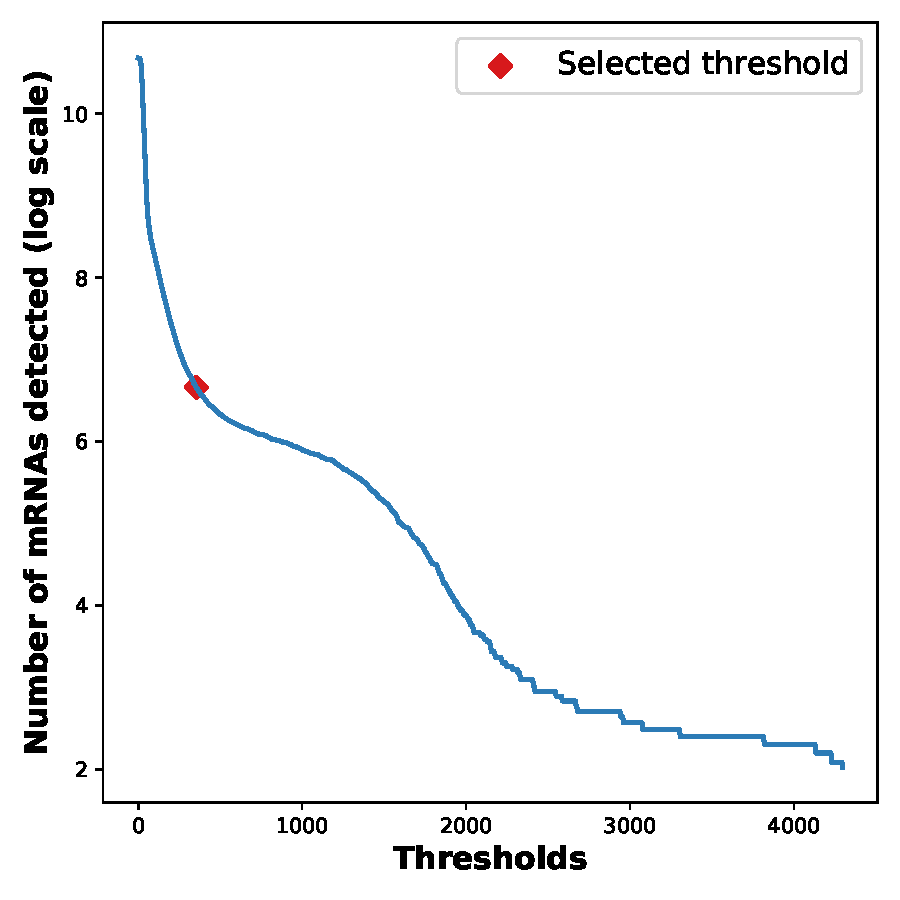
\includegraphics[width=0.33\textwidth]{figures/chapter2/elbow_curve_real}
	\caption[Elbow curve]{Elbow curve}
	\label{fig:elbow_detection}
	\end{center}
\end{wrapfigure}

We know that the major discriminative feature between spots originating from \ac{mRNA} and those from off-site binding of oligos is their intensity: real \ac{mRNA}s have significantly higher intensity values since an \ac{mRNA} molecule is targeted by multiple oligos.
Conversely, the actual shape and size of true \ac{mRNA}s and false positives is not necessarily different (see Figure~\ref{fig:filters_detection}).
In the Figure~\ref{fig:elbow_detection}, we plot the relation between different thresholds and the number of selected spots (with a log scale).
We observe a sharp and monotone decrease in the number of detected spots with increasing detection threshold.
The \emph{spots} removed are mostly background noise at these low threshold levels.
Actual spots are too bright to be filtered out.
At the opposite, if we increase the threshold too much, we start removing real spots and the sensitivity of the detection decreases.

In addition, we assume that wrong detections due to noise are much more frequent than actual \ac{mRNA}s.
This is a reasonable assumption, as off-site binding of a low number of probes is frequent.
This means that the decrease in spot number when the threshold increases should be large and relatively steady.
As soon as the number of removed spots by a further increase drops dramatically (see red point in Figure~\ref{fig:elbow_detection}), we can assume that we are reaching a point where we have removed most of the low-intensity noise and start removing spots originating from real \ac{mRNA}s.
We can thus argue that the right threshold value is reached when the reduction in spot number is beyond this first steep decrease and reaches a \emph{plateau}.
This plateau is reached when the tangent's slope equals the average slope of the curve (for the first time).
We have observed that even if this plateau is less pronounced than in Figure~\ref{fig:elbow_detection}, for instance if there is a particularly high level of noise, an abrupt change in the slope of the curve is still identifiable.
This difference of slope describes a clear separation between the regimes of overdetection and underdetection.
Additional elbow curves can be observed in appendix~\ref{sec:appendix_detection}, with different conditioning.\\

\begin{minipage}{0.9\textwidth}
\begin{lstlisting}[language=Python]
import bigfish.detection as detection

# spot detection with automated thresholding
spots, threshold = detection.detect_spots(
    images=smfish,
    return_threshold=True,
    voxel_size=(300, 103, 103),  # in nanometer
    spot_radius=(350, 150, 150))  # in nanometer
\end{lstlisting}
\end{minipage}

\subsection{Managing high spot density}
\label{subsec:dense_decomposition}

A second challenge in spot detection is the presence of clustered spots and high density areas, like active transcription sites or \ac{RNA} foci.
The method described above in~\ref{subsec:spot_detection} works well with isolated spots.
When spots are agglomerated, they might not be possible resolve anymore.
In practice, an accumulation of spots looks like a large and bright fluorescent region where our detection will underestimate the number of individual spots.

One option might be to use blob detection at different scales~\cite{walt_scikit-image_2014}, which would allow to identify these clusters as one spot.
However, we could still not represent them as an agglomeration of individual spots.
In \emph{bigfish.detection} we adapt the solution proposed in a previous version of MATLAB FISH-quant~\cite{mueller_fish-quant_2013, samacoits_computational_2018}.
We handle high spot density regions in two independent steps:

\begin{itemize}
	\setlength\itemsep{0.1em}
	\item In order to deal with \ac{RNA} underdetection in dense regions, we identify potential dense regions and decompose them into individual spots.
	This step increases the number of detected spots in the image (see figure~\ref{fig:dense_decomposition}).
	\item For subsequent analysis of the presence of clusters, we detect \ac{RNA} clusters by applying a clustering algorithm to the \ac{RNA} point cloud.
	This step can be performed with or without the dense region decomposition.
\end{itemize}

While somehow related, we stress that the first step tackles a technical issue of underdetection, while the second step allows us to separately define \ac{RNA} clusters for further analysis, as the number of clusters is an important feature of \ac{RNA} localization.

\subsubsection{Dense region detection}

\begin{wrapfigure}{R}{0.35\textwidth}
	\begin{center}
		
\includegraphics[width=0.33\textwidth]{figures/chapter2/reference_spot}
	\caption[Reference spot]{Reference spot}
	\label{fig:reference_spot}
	\end{center}
\end{wrapfigure}

The first step consists in localizing regions in the image with a high density of spots.
We know that for such regions our detection might miss several spots.

We remove the low-frequency noise from the image by subtracting its background intensity.
The latter is approximated with a large Gaussian filtering.
From this image we then extract the detected spots and compute the median spot signal.
This median signal allows us to define criteria for the identification of high density regions.
We expect high density regions to be brighter than individual spots, so they should at least be brighter than the median spot intensity.
A second criterion is the size of the regions.
Furthermore, they should be larger than an individual spot.
To match these criteria, we first threshold the denoised image with the median spot intensity, then we apply a connected component algorithm~\cite{wu_connected_component_2005} to the binary mask obtained.
Each group of connected pixels represents a region.
Because the mask is the result of a thresholding above the median spot signal, every region (or connected component) with at least 2 pixels are larger and brighter than the median spot for this image.

\subsubsection{Dense region decomposition}

The candidate regions can contain one individual \ac{RNA} spot brighter than the average, but they can also contain one large spot, corresponding to an agglomeration of very close \ac{RNA}s.
We reuse the denoised image and aggregate the detected spots to compute a reference spot like in Figure~\ref{fig:reference_spot}.
By default this reference is the median spot, but another percentile can be chosen.
We fit a Gaussian signal on the reference spot.
This model can then be used to simulate new spots.

The decomposition process consists in populating our candidate regions by simulating as many spots as possible until we match the pixel intensity we observe.
Starting with an empty image, we iteratively add a new simulated spot in the region until we minimize the residual sum of square (RSS):

\begin{equation}
	{\displaystyle \operatorname{RSS} = \sum _{x, y}(\hat{f}(x, y) - f(x, y))^{2}}
\end{equation}

\noindent
with $\hat{f}(x, y)$ the simulated image intensity and $f(x, y)$ the denoised image.

\begin{figure}[]
    \centering
    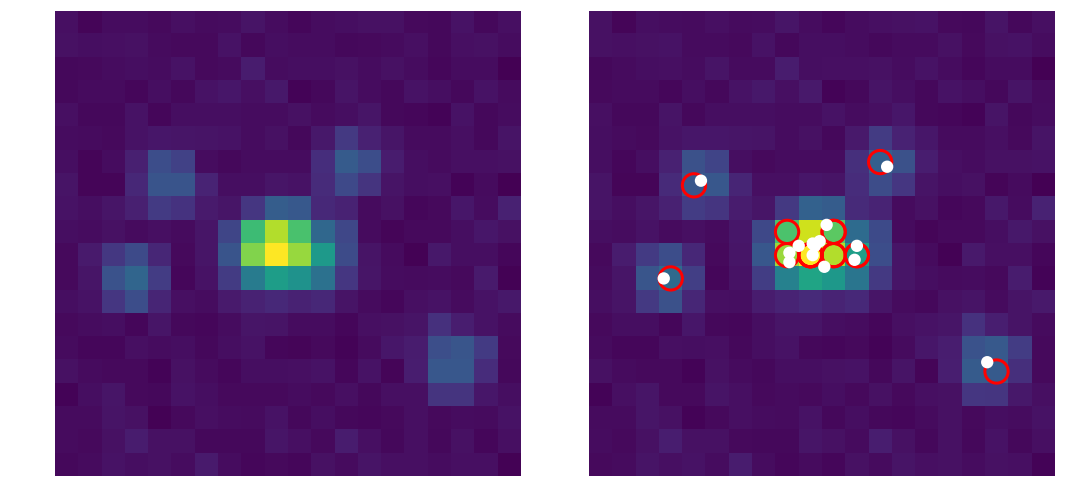
\includegraphics[width=1\textwidth]{figures/chapter2/plot_dense_decomposition}
    \caption[Example of dense region decomposition]{Decomposition results.
	(\textit{Left}) Original smFISH image zoomed in a dense region.
	(\textit{Right}) Detected spots in \textit{red} and actual clustered spots in \textit{white}}
    \label{fig:dense_decomposition}
\end{figure}

\subsubsection{Cluster detection}

The second (independent) step consists in applying a clustering algorithm on the spatial positions, in order to identify clusters according to a clearly understandable, biological meaningful definition, only based on spatial coordinates.

To this end we use a DBSCAN algorithm~\cite{ester_density-based_1996, scikit-learn}.
Two parameters need to be set: a minimum number of spots $k$ and a threshold distance $d$.
Every pair of \ac{RNA}s closer than $d$ are connected.
If an \ac{RNA} is connected to at least $k$ neighbors \ac{RNA}, it's a \emph{core sample} and with its connections it defines a cluster.
Such a method allows us to detect clusters as ''areas of high density separated by areas of low density''\footnote{\url{https://scikit-learn.org/stable/modules/clustering.html}}.

Different users might may have a different definition of what they expect to be a cluster.
For the rest of the manuscript and throughout our studies, we usually consider a minimum group of 4 or 5 \ac{RNA}s within a radius of 350nm.
These are the default parameters in \emph{bigfish.detection} and the ones we use in Figure~\ref{fig:detection_results}.\\

\begin{minipage}{0.9\textwidth}
\begin{lstlisting}[language=Python]
import bigfish.detection as detection

# dense decomposition
spots_post_decomposition, _, _ = detection.decompose_dense(
    image=smfish,
    spots=spots,
    voxel_size=(300, 103, 103),  # in nanometer
    spot_radius=(350, 150, 150))  # in nanometer

# cluster detection
spots_post_clustering, clusters = detection.detect_clusters(
    spots=spots_post_decomposition,
    voxel_size=(300, 103, 103),  # in nanometer
    radius=350,  # in nanometer
    nb_min_spots=4)
\end{lstlisting}
\end{minipage}

\subsection{Going beyond pixel accuracy}
\label{subsec:subpixel}

Two additional methods for reaching subpixel accuracy have been integrated in FISH-quant.
They were already present in the first version of FISH-quant~\cite{mueller_fish-quant_2013}.

\subsubsection{Subpixel fitting}

So far, the spot detection and the dense region decomposition and the cluster detection return coordinates with pixel accuracy.
In our applications, we were only interested in overall \ac{RNA} distribution, but for some applications, subpixel accuracy is critical.
Such error can be observed in the Figure~\ref{fig:dense_decomposition} between the detected spots (with pixel accuracy) and the ground truth (with subpixel accuracy).

The possibility to refine the coordinate on individual spots solves this limitation.
For this, we loop over the detected spots, crop the image and fit a gaussian signal on each of them individually.
We then correct the spot coordinates with the coordinates of the fitted gaussian.
Obviously, such method might return inaccurate results in high density areas when spots can't be resolved.\\

\begin{minipage}{0.9\textwidth}
\begin{lstlisting}[language=Python]
import bigfish.detection as detection

# subpixel fitting
spots_subpixel = detection.fit_subpixel(
    image=smfish,
    spots=spots,
    voxel_size=(300, 103, 103),  # in nanometer
    spot_radius=(350, 150, 150))  # in nanometer
\end{lstlisting}
\end{minipage}

\subsubsection{Spot colocalization}

\begin{wrapfigure}{R}{0.35\textwidth}
	\begin{center}
		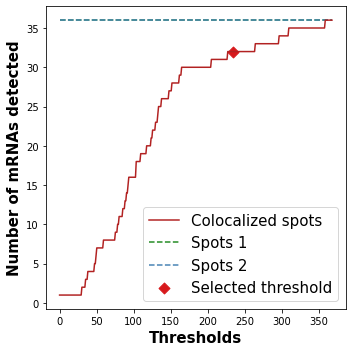
\includegraphics[width=0.33\textwidth]{figures/chapter2/colocalization_elbow}
	\caption[Impact of threshold on colocalization]{Impact of threshold on colocalization}
	\label{fig:elbow_colocalization}
	\end{center}
\end{wrapfigure}

Another method requested by the community is the possibility to detect adjacent spots in different channels then match their coordinates.
This could be the same \ac{RNA} detected with two different fluorescent probes or techniques in order to validate experimental protocols, or different \ac{RNA} for which we would like to investigate the co-localization.
As an example, in the Figure~\ref{fig:elbow_colocalization}, we detect colocalized spots between a sample of spots detected with pixel accuracy and the same sample with subpixel accuracy.

Our implementation is based on the methods published by ~\cite{CORNES_2022}.
First we compute the euclidean distance matrix between the two sets of spot coordinates, then we solve a linear sum assignment problem~\cite{crouse_linear_assignment_2016, 2020SciPy-NMeth}.
We obtain a matching between the two sets of spots, that minimizes the overall euclidean distance between assigned pairs.
Finally, we only keep pairs with a distance below a specific threshold.
The Figure~\ref{fig:elbow_colocalization} illustrates the impact of the threshold parameter on the number of colocalized spots.
Like for the spot detection, we implement our heuristic~\ref{subsec:spot_detection} to infer an optimal threshold if none is provided.\\

\begin{minipage}{0.9\textwidth}
\begin{lstlisting}[language=Python]
import bigfish.multistack as multistack

# spot colocalization
(spots_1_colocalized, spots_2_colocalized,
 distances) = multistack.detect_spots_colocalization(
	spots_1=spots_crop,
	spots_2=spots_subpixel_crop,
	voxel_size=(300, 103, 103))  # in nanometer
\end{lstlisting}
\end{minipage}

% \cite{lagache_statistical_2015}
% Colocalization methods are traditionally divided into pixel-based methods
% that measure global correlation coefficients from the overlap between pixel
% intensities in different color channels, and object-based methods that first
% segment molecule spots and then analyze their spatial distributions with
% second-order statistics.

\section{Evaluation with simulated spots}
\label{sec:detection_evaluation}

Finally we describe our evaluation of \emph{bigfish.detection}.
In addition to qualitative assessment of spot detection throughout our studies, we quantify the error from simulated images.
Performances for both spot and cluster detections are measured with different image qualities.

\subsection{Simulations}
\label{subsec:simulation}

To measure the error of a spot detection we need a ground truth.
A manual annotation of a regular 3D \ac{smFISH} image is intractable: such a strategy would be extremely time-consuming and prone to human error.
The alternative is to simulate realistic images of spots under different noise conditions in order to assess the performance of our algorithms and to study its limitations depending on image quality.
To this end, we built the simulation package \emph{simfish} that allows us to precisely control the level of noise and the number of spots we want to simulate in the image.

\subsubsection{Spot simulation}

The simulation process aims to return both an image and the ground truth coordinates of the spots we simulated.\\

\noindent
Our images are generated with three main steps:
\begin{enumerate}
	\item We randomly draw the number of spots and their localization.
	This is our ground truth.
	The number of spots is sampled from a Poisson distribution and the localizations from a uniform distribution all over the frame.
	Alternatively the number of spots can be set manually.
	\item For each spot in the image we simulate its pixel intensity.
	Instead of directly sample the intensity value from a Gaussian distribution, we reuse the simulation process from~\cite{bahry_rs-fish_2021}.
	With a Gaussian distribution centered on every spot, we simulate the average number of photons collected by each pixel in the image.
	The amplitude and the standard deviation of this Gaussian signals are manually or randomly predetermined.
	The final intensity of every pixel is then sampled from a Poisson distribution with the number of photons as expectation.
	\item (Optional) We add a background white noise to the entire image.
	It follows a Normal distribution centered around a predefined noise level.
\end{enumerate}

% add a schema of the cluster simulation process if necessary

The process detailed above generate spots with pixel accuracy.
A simulation with a subpixel accuracy follows the same steps, but with a larger image (4 to 20 times larger).
Before saving the image and the ground truth, it is downsized by local averaging.
The ground truth coordinates are adapted accordingly.

In order to produce a noisier image we can decrease the ratio between the spot amplitudes and the background noise.
A second option is to increase the variance of the different parameters: spot standard deviation and amplitude, background noise standard deviations.

\begin{figure}[]
    \centering
    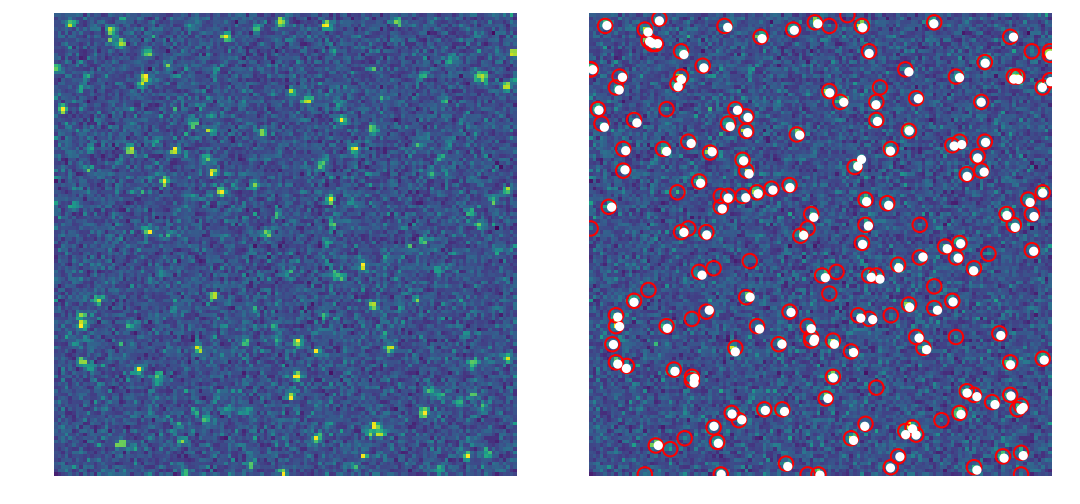
\includegraphics[width=1\textwidth]{figures/chapter2/plot_spot_detection}
    \caption[Simulation of noisy spots with \emph{simfish}]{Simulation of noisy spots with \emph{simfish}.
	(\textit{Left}) Original simulated image.
	(\textit{Right}) Detected spots in \textit{red} and actual spots in \textit{white}}
    \label{fig:spot_detection_high_noise}
\end{figure}

\subsubsection{Signal-to-Noise Ratio}

We can tune the different parameters mentioned to simulate spots with an increasing level of difficulty to detect.
To quantify the noise of an image and graduate the challenge it offers in terms of detection, we compute its \ac{SNR} for every spot.

\noindent
For a 2D image, we define the $\operatorname{SNR}$ of an image as the median of the $\operatorname{SNR_i}$ we compute for each spot $i$, such that:

\begin{equation}
	{\displaystyle \operatorname{SNR_i} = \frac{\max(a(x, y)) - \mu(b(x, y))}{\sigma(b(x, y))}}
\end{equation}

\noindent
with $\mu(.)$ the mean, $\sigma(.)$ the standard deviation, $a(x, y)$ the cropped spot image and $b(x, y)$ the spot background (a crop twice larger than the spot image).

In consequence, our measure of noise is based on the spot coordinates.
We quantify how distinct the spot is from its background.
A spot with a low amplitude or a noisy background will decrease the \ac{SNR} of the image.
To correctly quantify the image noise during our evaluation, we use the ground truth coordinates of the spots to compute the \ac{SNR}.
Indeed, a noisy image would impact the detection and bias the measure of noise itself.
We simulate different images with a range of \ac{SNR} between 2 and 26.
The higher the \ac{SNR} is, the better.

For example, in Figure~\ref{fig:spot_detection_high_noise} we simulate an extreme case with a highly noisy image (\ac{SNR} below 5).
On the right panel we can observe some contrasted background blobs misdetected as spot.
Despite a small amount of false positives, the detection remains correct in this badly conditioned image.

\subsubsection{Cluster simulation}

The user can also decide to simulate clusters.
In this case, the first step of our simulation process is adapted.
First the number of clusters and the number of spots per cluster are drawn from a Poisson distribution (or manually set).
The cluster centers are then localized like spots, with a uniform distribution over the entire image, or fixed at the center of the frame.
Finally, different spot localizations are randomly generated around the centers, using polar coordinates.
The result can be observed in Figure~\ref{fig:dense_decomposition} which is actually a simulated cluster.
In addition, several simulations are available in appendix~\ref{sec:appendix_simulations_spots}, with different conditioning.\\

\begin{minipage}{0.9\textwidth}
\begin{lstlisting}[language=Python]
import simfish as sim

# image simulation
image, ground_truth = sim.simulate_image(
	ndim=3,
	n_spots=100,
	image_shape=(128, 128),
	voxel_size=(100, 100, 100),  # in nanometer
	sigma=(150, 150, 150),  # in nanometer
	amplitude=5000,
	noise_level=300)
\end{lstlisting}
\end{minipage}

\subsection{Results}
\label{subsec:detection_results}

We simulated batches of 100 images with high, medium and low noise levels (roughly, with a \ac{SNR} below 5, between 5 and 15 and above 15).

\subsubsection{Impact of noise}

Our method is overall pretty robust.
If the image quality deteriorates, with a lower \ac{SNR} for example, our algorithms can return a moderate overestimation of detected spots.
This overestimation is estimated below 5\% and 10\% for images with a low or medium \ac{SNR} value, respectively.

These measures are illustrated on the left panel of Figure~\ref{fig:detection_error}.
We compared the number of spots detected with the actual number of spots simulated.
Each dot corresponds to one image.
For each noise regime, 100 images are generated.
Above the plain line, the detection overestimates the number of spots.
Logically, these overestimations increase with the noise level (and decrease with increasing \ac{SNR}).

On the right panel, we summarize the impact of noise with our detection technique.
Each dot represents again an image, with 100 simulated spots and a varying level of noise.
Below a \ac{SNR} of 5, with poorly contrasted spots, a fully automated detection might remain challenging.

\begin{figure}[]
    \centering
    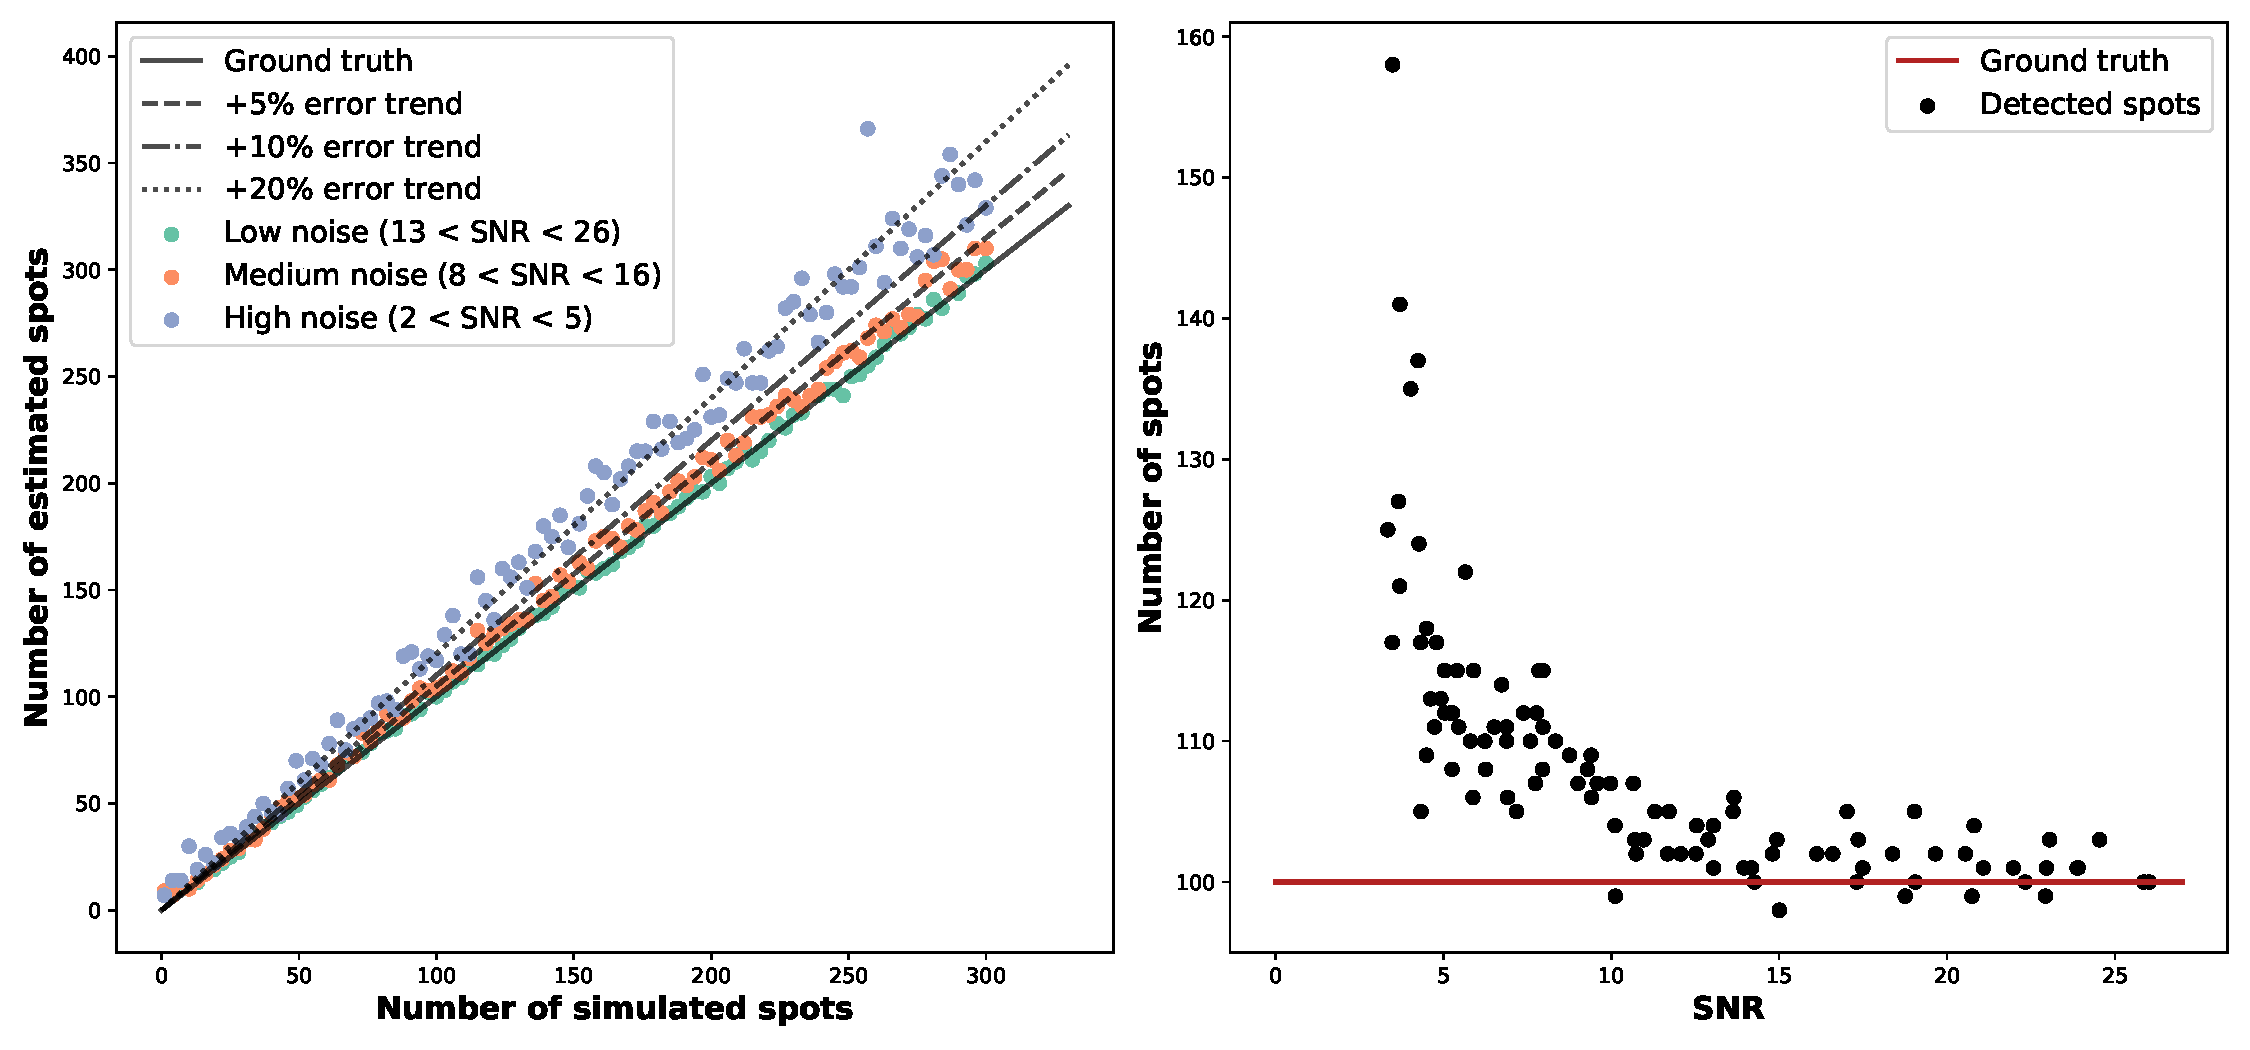
\includegraphics[width=1\textwidth]{figures/chapter2/fused_spot_detection_noise}
    \caption[Impact of noise on automated detection]{Impact of noise on automated detection.
	(\textit{Left}) Number of detected spots for different numbers of simulated spots.
	(\textit{Right}) Number of detected spots for different levels of noise (with 100 simulated spots)}
    \label{fig:detection_error}
\end{figure}

\subsubsection{Accuracy of the cluster detection}

We simulate images with a unique cluster in order to test the performance of our method to decompose the dense regions and detect the clusters.
Such images can be observed in appendix~\ref{sec:appendix_simulations_spots}.
In Figure~\ref{fig:cluster_results} we report the number of spots we estimate in the clusters.
Each dot represents an image with a cluster.
Our decomposition is quite robust with the noise level, even with the lower \ac{SNR} values.
However, for the largest clusters, with 15 spots or more, we tend to slightly underestimate the number of spots.
In this case, the average error is 1.6.
In comparison, with 5 spots and 10 spots per cluster, we measure an average error of 0.83 and 0.82, respectively.

\subsection{What if the PSF is not Gaussian?}
\label{subsec:psf}

In this chapter we assume our \ac{mRNA} spots can be modelled with a Gaussian signal.
This simplification was relevant during my PhD and did not lead to exaggerated errors in our different analysis.
However, it is always possible to exploit a more complex \ac{PSF} to fit with a specific spot signal.
To this end, the former \emph{psf} package\footnote{\url{https://github.com/cgohlke/psf/}} allows to generate more complex \ac{PSF} for specific fluorescent microscopic experiments.
Letting the user choose between different \ac{PSF} is an improvement that could be implemented in a future version of \emph{bigfish.detection} and \emph{simfish}.
In particular, this would modify the way we generate spot signal in our image simulations or in the decomposition of dense regions.

Eventually, if the \ac{PSF} differs greatly from a Gaussian signal, the spot detection itself could be impacted.
Indeed, two \ac{PSF}s from close spots could interfere and make the local peaks less distinct.

% potential references in PSF
% Electromagnetic diffraction in optical systems. II. Structure of the image field in an aplanatic system. B Richards and E Wolf. Proc R Soc Lond A, 253 (1274), 358-379, 1959.
% Focal volume optics and experimental artifacts in confocal fluorescence correlation spectroscopy. S T Hess, W W Webb. Biophys J (83) 2300-17, 2002.
% Electromagnetic description of image formation in confocal fluorescence microscopy. T D Viser, S H Wiersma. J Opt Soc Am A (11) 599-608, 1994.
% Photon counting histogram: one-photon excitation. B Huang, T D Perroud, R N Zare. Chem Phys Chem (5), 1523-31, 2004. Supporting information: Calculation of the observation volume profile.
% Gaussian approximations of fluorescence microscope point-spread function models. B Zhang, J Zerubia, J C Olivo-Marin. Appl. Optics (46) 1819-29, 2007.
% The SVI-wiki on 3D microscopy, deconvolution, visualization and analysis. https://svi.nl/NyquistRate
% Theory of Confocal Microscopy: Resolution and Contrast in Confocal Microscopy. http://www.olympusfluoview.com/theory/resolutionintro.html

\begin{figure}[]
    \centering
    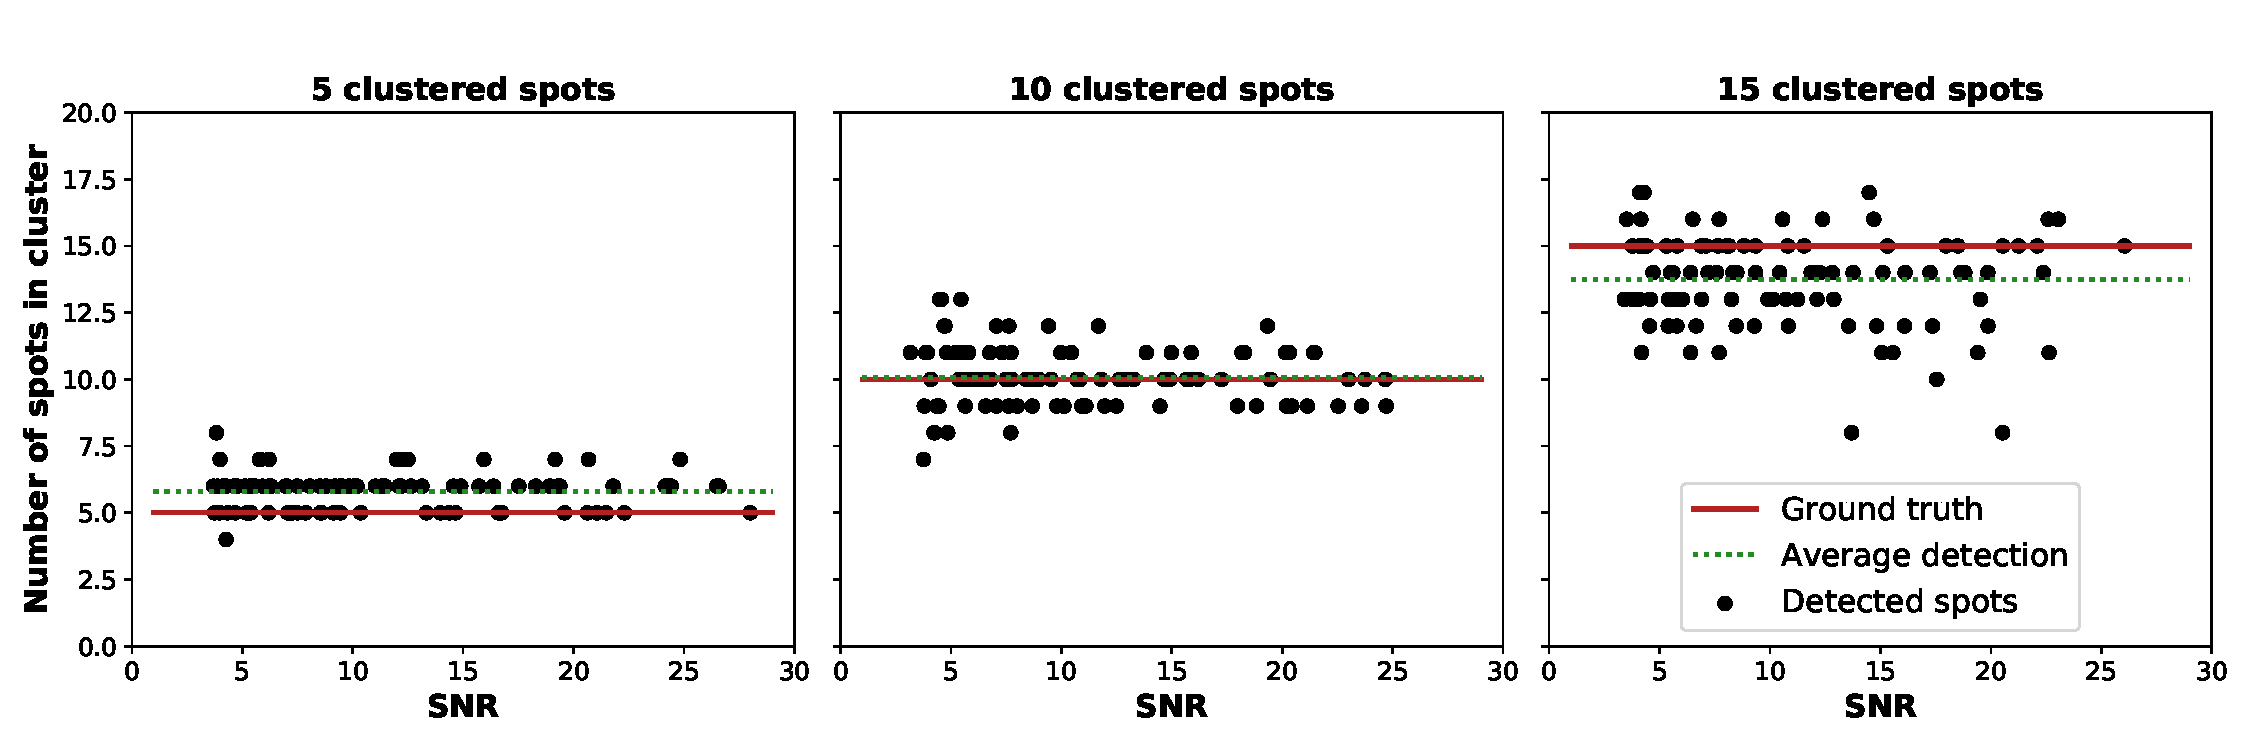
\includegraphics[width=1\textwidth]{figures/chapter2/cluster_along_noise}
    \caption[Evaluation of dense region decomposition]{Evaluation of dense region decomposition.
	 Number of spots estimated per cluster for different levels of noise and respectively 5 (\textit{left}), 10 (\textit{center}) or 15 (\textit{right}) simulated spots per cluster}
    \label{fig:cluster_results}
\end{figure}

\section{Conclusion}
\label{sec:detection_conclusion}

This chapter presents different methods from \emph{bigfish.detection} subpackage to perform spot detection in \ac{smFISH} images.
For this, we have re-implemented and extended algorithms first published in FISH-quant~\cite{mueller_fish-quant_2013}.
In particular, we have added a new scheme for thresholding that allows us to perform analysis of \ac{FISH} images without any manual intervention --- a pre-requisite for application at large scale.
Furthermore, we have provided methods and implementations for cluster detection and decomposition.
And finally, we have provided a framework for \ac{smFISH} image simulation in order to assess the performance of the various detection algorithms under different noise conditions.

Performance assessment of our methods for spot and cluster detection gave overall satisfying results, even for higher noise levels.
One limitation of the performance assessment we provide is the fact that it is based only on simulations.
Simulations clearly have many advantages for performance assessment, but also the inconvenience that they might not sufficiently represent domain shifts present in real data.
On the other hand, manual annotation is not a feasible alternative for this.
First, it is extremely time-consuming, and --- more importantly --- human annotators are also not necessarily in a position to decide whether a spot is a true \ac{mRNA} or not.
Another alternative that might provide additional insights and that we have not provided in this thesis, is a double-color \ac{FISH} against the same \ac{mRNA}.
However, also this assessment strategy is not perfect, as there is no guarantee that a given \ac{mRNA} will necessarily be marked in both channels.

With all the imperfections, we can nevertheless conclude that the performance of our detection algorithms is robust enough to be applied on a high content screening experiment.
Of course, several improvements are still possible.
We can expand the \ac{PSF} options as explained in~\ref{subsec:psf}.
Some alternative detection techniques that were published recently claim a better accuracy or faster runs like~\cite{bahry_rs-fish_2021, bouilhol_deepspot_2022}.
However, we feel that today, it is difficult to conclude on this, as performance assessment is not standardized, and the field is clearly lacking a general benchmarking strategy.
But in general, it would be another important step to provide Python implementations of these methods, and integrate them in FISH-quant v2.

% https://github.com/PreibischLab/RS-FISH/tree/master/documents/tool_comparison_for_paper % 4600 15
%%!TEX root = ../main.tex

\graphicspath{{./figures/chapter3/}}

\chapter{Single-cell segmentation}
\label{ch:chapter3}

\minitoc
\newpage

In this chapter, I review different techniques for nucleus and cell segmentation.
Recently, the solutions proposed to solve this problem have considerably improved, driven by the wave of deep learning models.

After a brief review of the literature in the first part, I describe the methods implemented in \emph{bigfish.segmentation} in a second part.
These methods are published in the paper~\cite{Imbert_fq_2022}:

\begin{center}
	\color{green}
	A. Imbert, W. Ouyang et al. (2022), \textit{FISH-quant v2: a scalable and modular tool for smFISH image analysis}, RNA, pp. $\operatorname{786--795}$, iSSN: $\operatorname{1355--8382, 1469--9001}$.
\end{center}

In a third part, I briefly present two projects for which I have contributed with the objective to boost segmentation efficiency, either by improving the consistency of segmentation masks or by reducing the number of training examples needed.
The former is a preliminary work with incomplete results; the latter was published at the ECCV Bioimage Computing Workshop (BIC)~\cite{Bonte_2022}:

\begin{center}
	\color{green}
	T. Bonte, M. Philbert et al. (2022), \textit{Learning with minimal effort: leveraging in silico labeling for cell and nucleus segmentation}, in 2022 European Conference on Computer Vision (ECCV 2022) Workshop on BioImage Computing \textit{(to be published)}.
\end{center}

\section{Segmentation of nuclei and cells in fluorescence microscopy}
\label{sec:segmentation_introduction}

First, I describe the segmentation task that comes in different flavors. 
%, its input and the expected output.
Then, I review different methods that address nucleus and cell segmentation, especially deep learning based models.

\subsection{Computer Vision for cell segmentation}
\label{subsec:segmentation_instance_introduction}

The most useful tasks of Computer Vision in bioimage analysis are classification, object detection and object segmentation. 
%Computer vision can be decomposed in several tasks.
Classification is concerned with predicting a label for a given input image. 
%A classification model classifies images according to whether they have a targeted object in their frame.
Object detection aims at both classifying and localizing objects inside an image, where localization normally amounts to returning the coordinates of the bounding box of the object. 
Of note, object detection is designed to detect several instances of the same object class. 
%A detection model goes further and usually returns coordinates of the bounding box of the object.
%Such model can localize the object in the image but also detect several occurrences of the same object class.
Finally, a segmentation model returns returns a mask for the targeted objects.
If the model does not distinguish between instances of the same object class, it is a semantic segmentation model. 
Semantic segmentation resumes to pixel classification, where each individual pixel is classified into object or background (or potentially different foreground classes). 
In contrast, the most important segmentation problem in bioimage analysis is instance segmentation, where the model not only distinguishes between foreground and background but also between different objects. This kind of models is of particular interest for cell and nuclei segmentation, as both cells and nuclei often touch each other. 

An example of instance segmentation with nuclei and cells is shown in Figure~\ref{fig:instance_segmentation_example}.
A unique identifier and segmentation mask are returned for every instance.
In Figure~\ref{fig:instance_segmentation_example}, segmentation masks have been postprocessed such that a nucleus has the same identifier as its corresponding cell.

\begin{figure}[]
    \centering
    
\includegraphics[width=\textwidth]{figures/chapter3/instance_segmentation}
    \caption[Example of instance segmentation]{Example of instance segmentation.
	(\textit{Left}) Nucleus masks.
	(\textit{Right}) Cell masks.
	Every nucleus and cell instance has a different colored mask.
	Plot built with \emph{bigfish}}
    \label{fig:instance_segmentation_example}
\end{figure}

For the rest of the chapter, I only consider 2D segmentation.
%This constraint often implies to project the input images in 2D.
Models for 3D segmentation are emerging in the literature, but as manual annotation in 3D is complex and time-consuming, it does not seem an interesting option for our applications. 

 % ground truth is particularly complex, 

% but are usually directly adapted from a 2D version or they require some difficult manual annotation in 3D images.

A specific difficulty with instance segmentation, compared to semantic segmentation, is the need to discriminate between two adjacent instances.
In case of cell segmentation, this is particularly important. For instance, if we wish to quantify cell shape properties or assess the number of \ac{RNA} inside a cell, it is essential to be able to extract the contours of the cells with high accuracy. 

%even more important because relevant spatial information can be extracted along the cell membrane.
%This highlights the need to be able to perform efficient segmentation to address specific phenotypes in cluttered cell images.

Even though it might be tempting in some applications to omit the cell segmentation step altogether and to classify images of entire cell populations~\cite{Godinez2017}, I believe that cell and nucleus segmentation add great value to the analysis pipelines as they enable one to assign every phenotype or pattern detected in an image to an individual cell. Segmentation is thus the corner stone of any single-cell analysis.
Instance segmentation is a critical step to capture information at the cell level, especially when the biological mechanism studied exhibits a high intracellular heterogeneity.

\subsection{Related work}
\label{subsec:segmentation_related_work}

\subsubsection{From mathematical morphology\dots}

Fluorescence Microscopy has been specifically designed to provide images, where structures of interest appear with high contrast, and irrelevant structures are invisible. This can greatly simplify the segmentation task, in particular when objects are isolated and can be easily discriminated from the background.
This is often the case for nuclei, with DAPI channel.
Therefore, a first approach, simple but often successful, is to threshold the image to discriminate instances from background, then identify each disconnected mask with a unique identifier to label the objects.
To avoid manual setting of the threshold for each image, automatic methods based on histogram intensity analysis can be exploited, such as Otsu thresholding~\cite{Otsu_1979}.
For clustered nuclei or images with crowded cells, this method does not work and more complex algorithms are needed.

A popular segmentation method for segmentation of nuclei and cells is the watershed algorithm~\cite{Beucher1979,Serra1983,Vincent_1991}.
An image is interpreted as a local topography (higher values are peaks and crests, lower values valleys and basins).
There are several variants of this method, but basically the algorithm requires three elements: the starting points from which we flood the image (the markers or seeds; the local minima as default), a relevant topographic representation of our image where the boundaries of the object have higher pixel values, and optionally a binary mask limiting the flooding area (the mask). The Watershed algorithm simulates a flooding where pixels are subsequently added to the extending seed regions in such a way that pixels with lower value are always processed first. Object boundaries are found where the extending seed regions meet. 

This is an attractive strategy for cell segmentation: we can use a previous result of nucleus segmentation as markers and the cell image with any fluorescent label to which we apply the watershed algorithm (possibly with its intensity values inverted such that background pixels get higher values).
Unfortunately, if we miss some nuclei at the beginning, the error impacts the rest of the computational pipeline: not only we miss potentially interesting cells, but we also wrongly assign cytoplasmic regions to cells where they do not belong.
For this reason, it is important that the nuclei detection returns accurate results.

Many other segmentation methods have been proposed in the computer vision literature.
Superpixels approaches, for instance, partition the image into multiple homogeneous regions with enforced compactness~\cite{Ren_2003}.
Low-level segmentation algorithms such as watershed itself can help form these regions by clustering pixels together~\cite{Machairas_2014}.
The segmentation task can also be addressed from the boundaries point of view.
Active contour models (or snake) rely on energy minimization techniques to deform a spline curve until it delineate the object outline~\cite{kass_snakes_1988}.

For most segmentation benchmarks, these methods have been outdated in recent years, with the emergence of deep learning models trained on large and diverse datasets.
However, mathematical morphology methods remains relevant for some use cases, especially to address unusual image modality or specific shape to segment.
Most importantly, these methods do not require manual annotation, which is often a bottleneck for medical or biological image segmentation.
Eventually, such algorithms can also inspire new learning-based models, like Deep watershed model that predicts a watershed energy map before extracting object instances from it~\cite{Bai_2017_CVPR}.

\subsubsection{\dots to deep learning models}

% recent successes
Deep learning literature for image segmentation has provided several powerful and consistent models.
Mostly based on \ac{CNN}, they have dramatically boosted computer vision applications.
This trend keeps influencing bioinformatics as well.

% U-Net
One of the seminal neural networks proposed for biomedical segmentation is U-Net~\cite{Ronneberger_unet}.
The network has a U-shaped architecture with an encoder and a decoder.
The former combines convolutional layers, non linear activation functions (ReLU) and max pooling operations to reduce spatial information and expand feature information.
The latter includes upsampling layers to return an output segmentation map that is postprocessed in order to build a (semantic) segmentation mask.
This architecture is now a classic and it is vastly reused by more recent work like StarDist~\cite{schmidt2018}, which is trained to predict star-convex polygons for each nucleus or cell instance.

% importance of dataset
One the main limitations of deep learning methods is the need for a large amount of annotated images to train the models.
Some of the first successful applications of \ac{CNN} involved large annotated dataset of natural images like ImageNet~\cite{Deng_2009} or COCO dataset~\cite{Lin_2014}.
Recent publications in biomedical segmentation include sometimes both a trained model and a release of an important dataset with segmented nuclei or cells.
For example, the research community benefits from an online challenge organized in 2018 about nucleus segmentation: the 2018 Data Science Bowl\footnote{\url{https://www.kaggle.com/c/data-science-bowl-2018}}.
This competition includes a large collection of images with different modalities (histopathology, fluorescence microscopy).

% NucleAIzer
NucleAIzer~\cite{hollandi_nucleaizer_2020} proposes a model inspired by the winning solutions of the 2018 challenge and trained on the released dataset.
It combines Mask R-CNN~\cite{He_2017_ICCV} and U-Net.
Post competition, it outperforms all the submitted methods of the competition.

% Cellpose
Cellpose~\cite{stringer_cellpose_2021} proposes a U-Net based model for nucleus and cell segmentation.
The network is trained to predict horizontal and vertical gradients of the topological cell map.
These gradients form a vector field where each pixel ''belonging to a given cell can be routed to its center''.
By grouping pixels converging to the same regions, individual instances can be identified.
Most importantly, authors have collected and manually annotated 608 cell images with various modalities.
Currently, this solution appears to be one of the most efficient.
The authors have extended their method by training it with several specialized datasets like TissueNet~\cite{Greenwald_2022} or bacteria images~\cite{cutler_omnipose_2022}.

% adaptated from natural image model
Another important factor for progress in segmentation is the state of the literature on natural image segmentation.
Indeed, several methods published for biomedical segmentations are inspired from a previous model trained on natural images.
For example, NucleAIzer reuses Mask R-CNN.
It is a \ac{CNN} which efficiently suggests regions of interest, detects object instances within these regions and performs instance segmentation with a fully convolutional branch.
When released in 2017, the model was state-of-the-art on the COCO dataset.
This relationship can also be observed with EmbedSeg~\cite{Lalit_2021} directly inspired by~\cite{Neven_2019_CVPR}.

\section{Nucleus and cell segmentation}
\label{sec:segmentation_nuc_cell}

In this section, I first describe a dataset I have annotated in order to train a deep learning segmentation model.
Then, I detail the solutions implemented in \emph{bigfish.segmentation} to segment both nuclei and cells.
In addition, several postprocessing functions are presented to refine any segmentation results.

\subsection{A new multichannel dataset}
\label{subsec:segmentation_data}

\begin{figure}[]
	\centering
	\minipage{0.5\textwidth}
		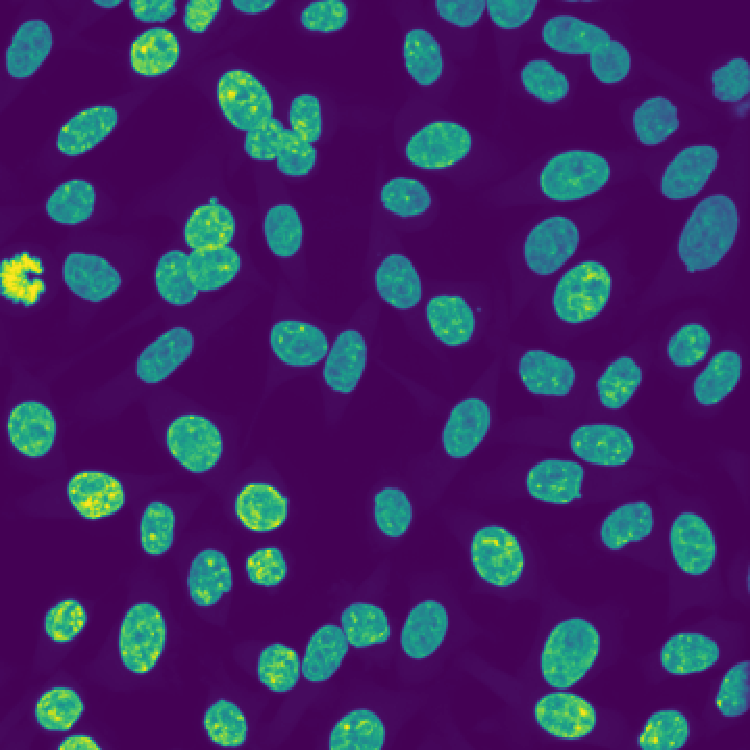
\includegraphics[width=0.95\linewidth]{figures/chapter3/dapi_BICD2}
		\subcaption{DAPI channel}
		\vfill
		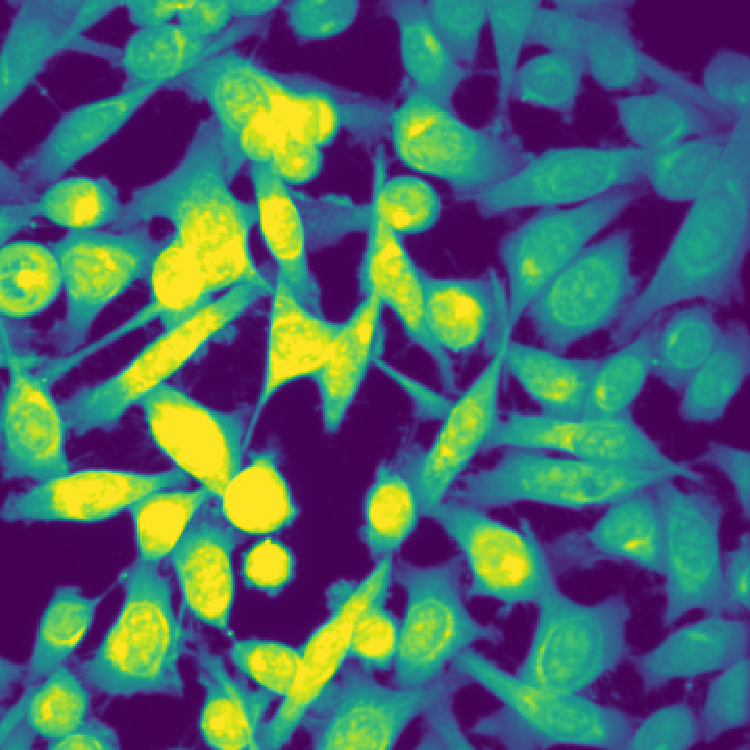
\includegraphics[width=0.95\linewidth]{figures/chapter3/cellmask_BICD2}
		\subcaption{CellMask\textsuperscript{\texttrademark} channel}
	\endminipage\hfill
	\minipage{0.5\textwidth}
		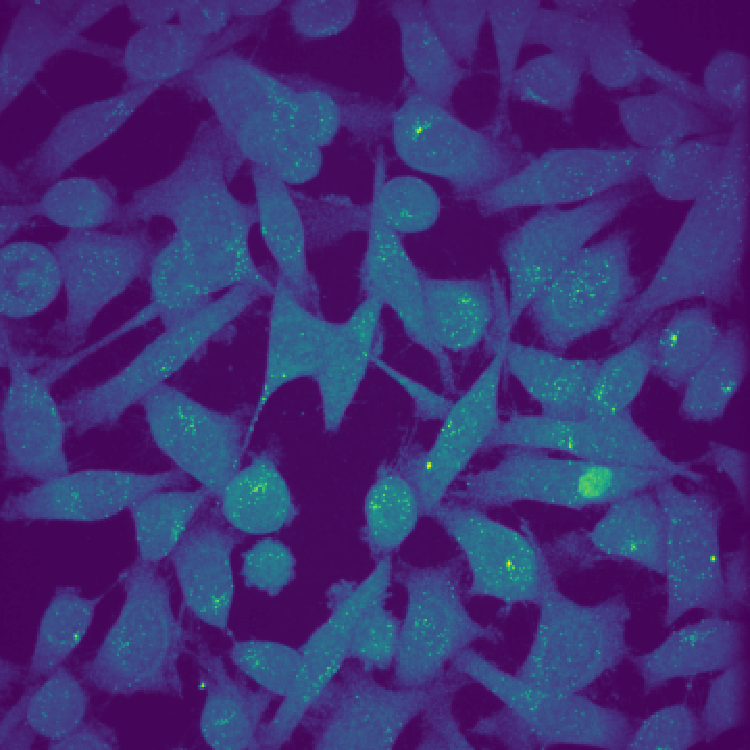
\includegraphics[width=0.95\linewidth]{figures/chapter3/smfish_BICD2}
		\subcaption{smFISH channel}
		\vfill
		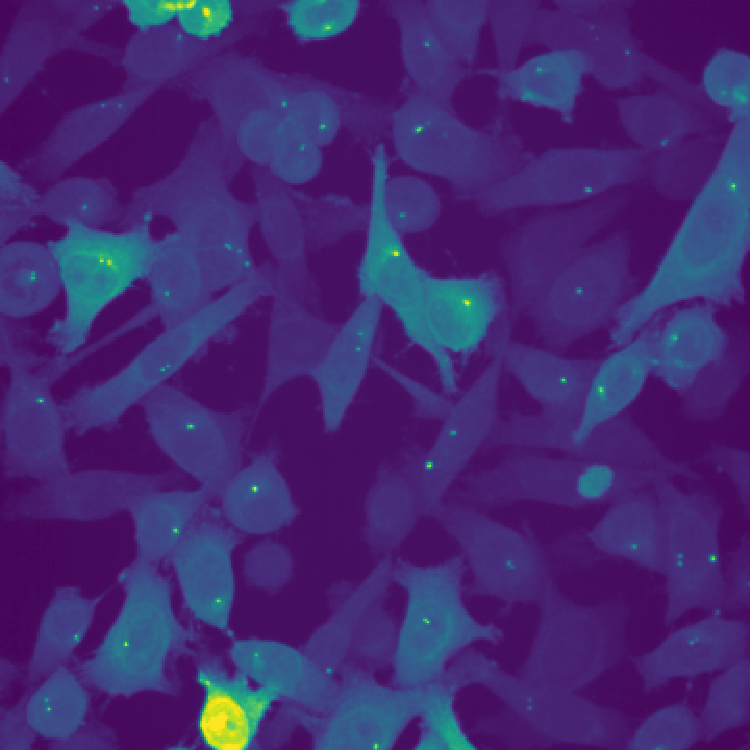
\includegraphics[width=0.95\linewidth]{figures/chapter3/gfp_BICD2}
		\subcaption{GFP channel}
	\endminipage
	\caption[Segmentation dataset]{Multichannel annotated images for nucleus and cell segmentation.
	Images are projected in 2D.
	Plot built with \emph{bigfish}}
	\label{fig:annotated_dataset_segmentation}
\end{figure}

I reuse the 4-channel images from~\cite{safieddine_choreography_2021} to build an annotated dataset for the segmentation task.
I randomly sample 180 \ac{FoV}s.
Each image includes one channel adapted for nucleus segmentation (DAPI) and three channels adapted for cell segmentation (\ac{smFISH}, CellMask\textsuperscript{\texttrademark} and a \ac{GFP} marker for the centrosome).
An example of these images is illustrated in Figure~\ref{fig:annotated_dataset_segmentation}.
The ground truth annotation is obtained in two steps: I pre-segment nuclei and cell with a Cellpose model~\cite{stringer_cellpose_2021}, then I manually correct these predictions.
In total, 4,026 cell instances are segmented, with their relative nucleus.

The initial goal for this dataset is to train segmentation models or compute some experiments to evaluate their consistency.
In particular, two kinds of evaluations can be tested.
The first one is about the consistency between nucleus and cell segmentation, two tasks often performed independently.
The dataset is annotated such that each instance has a nucleus and a cell mask, matching together.
This also enables a potential joint training of nucleus and cell segmentation.
The second possible evaluation is about the input heterogeneity.
Here, the cell related channels come from three different modalities of acquisition.
A priori, a model trained on CellMask\textsuperscript{\texttrademark} should be more efficient, but because this label is not always available in an experimental setup, it is interesting to train models robust enough to identify cells from different channels.

\subsection{Nucleus segmentation}
\label{subsec:segmentation_nuc}

Nucleus segmentation is usually the first task in cellular image analysis, applied on a DAPI channel for example.
An error during this step can propagate to the rest of the analysis, if the cell segmentation and identification is based on an initial nucleus segmentation.
In particular, missed nuclei or split nuclei are the kind of errors I want to prevent.
Even if thresholding technique is implemented in \emph{bigfish}, a simple deep learning model is also available for nucleus segmentation.

\subsubsection{A 3-class deep learning model}

The model is described in~\cite{Imbert_fq_2022}.
It uses an encoder-decoder architecture like U-Net~\cite{Ronneberger_unet}, with 4 downsampling stages.
In total, the spatial resolution of the input image is divided by 16 at the bottom of the model.
For each stage, I implement residual blocks, mimicking Cellpose model~\cite{stringer_cellpose_2021}.
Lastly, the upsampling stage is implemented following deconvolution techniques from~\cite{odena2016deconvolution} to prevent any checkerboard artifacts.

The nucleus segmentation problem is address like a pixel-wise classification problem with three classes: background, foreground and nuclear boundary.
My model assigns one of these three classes to each pixel.
The returned final mask is the foreground predicted surface, postprocessed with a dilation of 1 pixel.
This model is trained on the DAPI channel from the annotated dataset presented in~\ref{subsec:segmentation_data}, with a categorical cross-entropy loss.\\

\begin{minipage}{0.9\textwidth}
\begin{lstlisting}[language=Python]
import bigfish.segmentation as segmentation

# load pretrained model
model_nuc = segmentation.unet_3_classes_nuc()

# instance segmentation
nuc_label = segmentation.apply_unet_3_classes(
    model=model_nuc,
	image=image_nuc,
	target_size=256,
	test_time_augmentation=True)
\end{lstlisting}
\end{minipage}

\subsubsection{Multiple rounds of segmentation}

In \emph{bigfish.segmentation}, I implement a method to remove segmented nuclei from a DAPI channel, in order to perform a second round of segmentation.
This technique based on morphological reconstruction is useful if the employed segmentation method misses too many nuclei at first try.
These failures can be due to a heterogeneous DAPI signal between cells, to the presence of adjacent nuclei or instances with unusual shape.
I proceed with the following steps for the removal:

\begin{enumerate}
	\setlength\itemsep{0.1em}
	\item I dilate the binary mask of the segmented nuclei.
	\item In the original DAPI image, every pixels outside of the dilated mask are set to zero.
	This includes the background and the potentially missed nuclei.
	\item I perform a morphological reconstruction~\cite{Robinson_2004} of the missing nuclei by small dilation.
	This dilation is constrained by the original DAPI image.
	A pixel cannot have a dilated value greater than its original intensity.
	This way, the background pixels keep a low intensity and the missed nuclei (brighter in the original image) are partially reconstructed by the dilation.
	The reconstructed image only differs from the original one where the nuclei have been missed.
	\item I subtract the reconstructed image from the original one to get an approximate image of the missing nuclei.
	The latter is used to threshold a binary mask of the missing nuclei and ultimately extract their original pixel intensity from the original image.
\end{enumerate}

\noindent
Finally, after a second round of segmentation, the two obtained nucleus segmentation masks can be merged together.
Surprisingly, repetitive application of the same segmentation model seems to help improving the final segmentation.
In particular, this technique is applied in~\cite{CHOUAIB_2020}.\\

\begin{minipage}{0.9\textwidth}
\begin{lstlisting}[language=Python]
import bigfish.segmentation as segmentation

# first attempt of segmentation (with missing nuclei)
#nuc_label_1 = model(nuc_image)

# remove segmented nuclei
remaining_nuc_image = segmentation.remove_segmented_nuc(
	image=nuc_image,
	nuc_mask=nuc_label_1)

# second attempt of segmentation
#nuc_label_2 = model(remaining_nuc_image)

# merge nucleus labels
nuc_label = segmentation.merge_labels(nuc_label_1, nuc_label_2)
\end{lstlisting}
\end{minipage}

\subsection{Cell segmentation}
\label{subsec:segmentation_cell}

Cell segmentation is often more difficult.
It can involve images with cluttered cells, fluorescent labels with different quality or labels not initially designed to visualize the cytoplasm (for example, the \ac{smFISH} channel).
In addition, cells can exhibit even more diversity in their morphological shapes than nuclei, and a successful method with HeLa cells could fail with bacteria images.

A watershed algorithm is available in \emph{bigfish.segmentation} to discriminate adjacent cells.
A previous nucleus segmentation mask is used as marker.
Instead of the color pixel, the grayscale level of fluorescence intensity is used as input image (potentially regularized with the distance map from nuclei).

\subsubsection{A revisited deep watershed model}

I also implement a deep learning solution for cell segmentation, inpired by Deep Watershed~\cite{Bai_2017_CVPR} and the use of distance maps for nucleus segmentation~\cite{Naylor_2019}.
Two models are tested, with the same backbone architecture previously presented for nucleus segmentation: an encoder-decoder convolutional neural network with residual blocks.

First model uses only one input image with cell information (in my case, CellMask\textsuperscript{\texttrademark}, \ac{smFISH} or \ac{GFP}).
This model predicts two outputs: a binary mask of cell surface (like in semantic segmentation tasks) and a distance map to cell edges.
I reuse these outcomes in a watershed algorithm and segmented nuclei as seeds in order to return a segmentation mask for every cell instance.
Model is trained with a combined loss averaging a binary cross-entropy loss for the surface prediction and a mean absolute loss for the distance map.

Second model uses two input images, one for the nuclei and one for the cells.
In addition to the two previous output images, it predicts a third output: a distance map to nucleus edges.
Cell instances are obtained with the same strategy as above, namely by application of a watershed algorithm.
The idea is to add an input information about the nuclei and to force the model to take it into account by returning a nucleus related prediction.
I speculate this would make cell segmentation more accurate.
Finally, in \emph{bigfish.segmentation} the second model is implemented, with a double input strategy.\\

\begin{minipage}{0.9\textwidth}
\begin{lstlisting}[language=Python]
import bigfish.segmentation as segmentation

# load pretrained model
model_cell = segmentation.unet_distance_edge_double()

# instance segmentation
cell_label = segmentation.apply_unet_distance_double(
    model=model_cell,
    nuc=image_nuc,
    cell=image_cell,
    nuc_label=nuc_label,
    target_size=256,
	test_time_augmentation=True)
\end{lstlisting}
\end{minipage}

\subsubsection{Postprocessing and refinement}

Regardless of the segmentation method applied, \emph{bigfish.segmentation} includes different methods to clean and refine the segmentation masks.
The most simple operations consist in smoothing the mask boundaries with a median filter, removing the small disjoint masks or filling holes within the segmented areas.
By subtracting an eroded segmentation mask to a dilated one, I can also prevent boundaries contact and delimitate segmented instances.
An example of such refined results is illustrated in Figure~\ref{fig:instance_segmentation_example}.
Lastly, after two independent nucleus and cell segmentations, a method matches every identified cell with the right nucleus.\\

\begin{minipage}{0.9\textwidth}
\begin{lstlisting}[language=Python]
import bigfish.segmentation as segmentation
import bigfish.multistack as multistack

nuc_label = segmentation.clean_segmentation(
	nuc_label=nuc_label,
	delimit_instance=True)
cell_label = segmentation.clean_segmentation(
	cell_label=cell_label,
	smoothness=7,
	delimit_instance=True)
nuc_label, cell_label = multistack.match_nuc_cell(
	nuc_label=nuc_label,
	cell_label=cell_label,
	single_nuc=False,
	cell_alone=True)
\end{lstlisting}
\end{minipage}

\subsubsection{Segmentation evaluation}

The main advantages of the available deep learning models in \emph{bigfish.segmentation} is to offer an efficient in-house segmentation solution, without the need to use another API, package or framework.
It is fast to apply and can be a relevant first solution to try.
However, for more challenging segmentation problems, FISH-quant v2 still enables the use of external resources like Cellpose or StarDist.

Both nucleus and cell segmentation models are trained with Adam optimizer~\cite{Diederik_2015} until validation loss does not improve anymore.
I evaluate them with the mean Average Precision.
I compute the \ac{IoU} score for each pair of predicted and ground truth instances (whose value ranges between 0 and 1).
Prediction matches the ground truth if the \ac{IoU} is above a specific threshold.
Therefore, for a given threshold, I can compute True Positives (instances matched correctly), False Positives (predicted instances matching nothing), False Negatives (ground truth instances missed) and the \ac{AP} score such that:

\begin{equation}
	{\displaystyle \operatorname{AP} = \frac{\operatorname{TP}}{\operatorname{TP} + \operatorname{FP} + \operatorname{FN}}}
\end{equation}

\noindent
The mean Average Precision is the average of the \ac{AP} score for different \ac{IoU} thresholds between 0.5 and 0.95.
A higher value indicates a better agreement between prediction and ground truth instances.

Results for my deep learning implementations are shown in Table~\ref{table:segmentation_results}.
Evaluation is performed on the multichannel dataset extracted from~\cite{safieddine_choreography_2021}.
As expected, best results for cell segmentation are obtained with CellMask\textsuperscript{\texttrademark} input, while \ac{smFISH} and \ac{GFP} channels yielded similar \ac{AP} scores.
Interestingly, the addition of nucleus information in input slightly improves cell segmentation results for the \ac{smFISH} and \ac{GFP} channels.

\begin{table}[]
	\centering
	\begin{tabular}{| c | c | c | c | c |}
		\hline
		Model & DAPI & CellMask\textsuperscript{\texttrademark} & smFISH & GFP\\
		\hline
		3-class U-Net & \textbf{0.6} & - & - & -\\
		Distance map U-Net & - & \textbf{0.66} & 0.59 & 0.58\\
		Distance map U-Net (double input) & - & 0.65 & \textbf{0.63} & \textbf{0.62}\\
		\hline
	\end{tabular}
	\caption[Segmentation results]{Segmentation results for different input channels.
	Computed score is the mean Average Precision, the higher, the better.
	Best models are bold.
	Evaluation is performed over 19 images}
	\label{table:segmentation_results}
\end{table}

\section{Improving cell segmentation}
\label{sec:segmentation_improvements}

I have contributed to two projects with the aim to improve specific aspects of biomedical segmentation.
The first one is a personal project and consists in developing a deep learning version of the active contour algorithm.
However, this work is not finished and it yields incomplete results, so here I only present the main idea.
The second project results in a publication~\cite{Bonte_2022}.
It leverages in-silico labelling protocol to pre-train segmentation models.

\subsection{Snake-like model}
\label{subsec:segmentation_snake}

This project tries to address potential failures between nucleus and cell segmentation when these two tasks are performed independently.
Sometimes the cell is correctly segmented, but not the nucleus, sometimes it is the opposite.
If I cannot match a nucleus with a cell, the whole instance is discarded.
In addition, nucleus is often far easier to segment than cell.

The idea is to propagate or extend the cell outline from the nucleus one.
I want to base cell segmentation on a previous successful nucleus segmentation.
This is kind of what is already happening with watershed algorithm when the nucleus is used as starting seed.

Inspired by active contour models, the goal is to deform a spline curve around cell instance, but instead of solving an energy minimization problem a neural network would predict the deformation of the polygon.
Such method has already been proposed for natural image segmentation like Deep Snake~\cite{Peng_2020_CVPR} or DANCE~\cite{Liu_2021}.
However, these models need to first detect the candidate object instance and then initialize the deformable polygon from the detected bounding box.
Their entire pipeline relies on the performance of a detection model.
In my case, the cell outline would be initialized from the nucleus outline (much easier to segment), before being iteratively distorted by a fully convolutional network.

\subsection{In silico pre-training}
\label{subsec:segmentation_insilico}

We leverage \ac{ISL} task to pre-train segmentation model and mitigate the need for annotated training images.
\ac{ISL} consists in predicting fluorescent labels from bright-field or transmitted-light images~\cite{christiansen_silico_2018, ounkomol_label_free_2018}.
We replace an invasive fluorescent labeling by a numerical and computational one, like illustrated in Figure~\ref{fig:example_insilico}.
Furthermore, fluorescent channels are limited in numbers (up to 4 or 5).
Therefore, the ability to predict cell morphology from a label-free channel would save fluorescent channels for another probe or stain.
More complex experiments are possible.

\begin{figure}[]
    \centering
    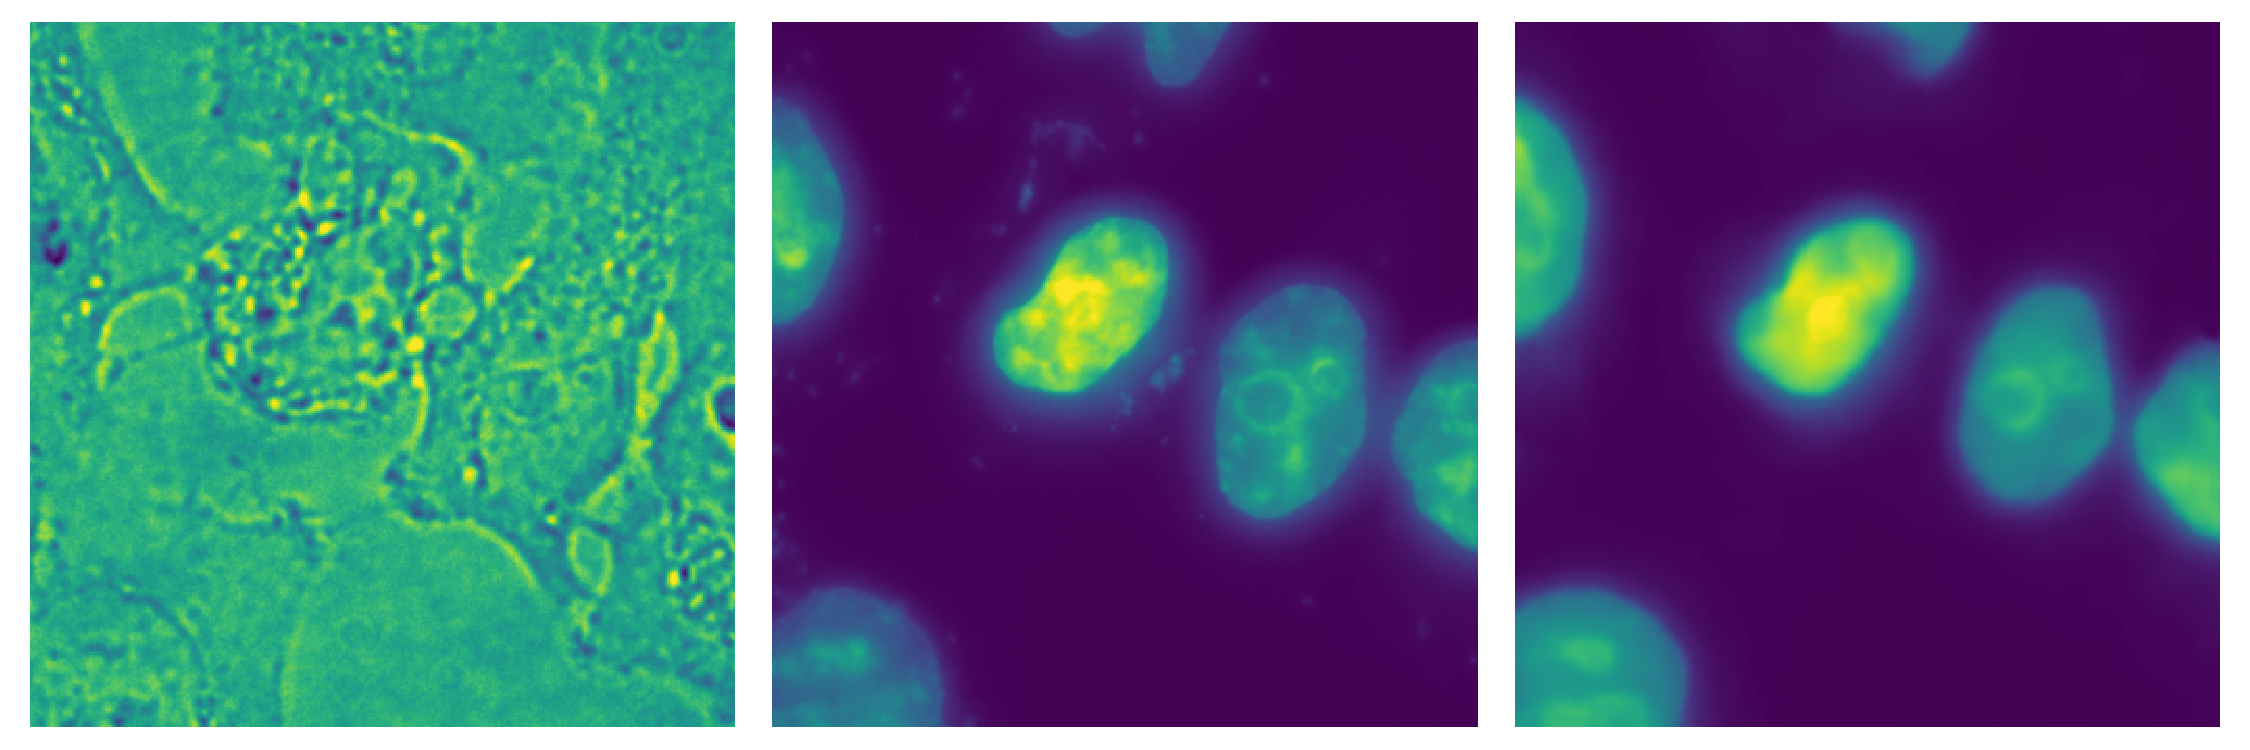
\includegraphics[width=\textwidth]{figures/chapter3/insilico_prediction}
    \caption[Example of in silico labeling]{Example of in silico labeling, from~\cite{Bonte_2022}.
	(\textit{Left}) Bright-field input image.
	(\textit{Center} Ground truth DAPI channel.)
	(\textit{Right}) Predicted DAPI}
    \label{fig:example_insilico}
\end{figure}

In~\cite{Bonte_2022}, we use the same model to perform \ac{ISL} and segmentation.
It is based on a U-Net architecture, with a DenseNet encoder branch~\cite{Huang_2017_CVPR}.
The first training on \ac{ISL} makes the model learn intermediate visual representations of the cell.
We speculate that these learned features are (partially) relevant for the segmentation task.
In this case, the following segmentation training should be more efficient.

In Figure~\ref{fig:results_insilico} we compare the \ac{IoU} score of the trained models for different training set size.
A second model pre-trained with a natural image classification task (from ImageNet~\cite{Deng_2009}) is also displayed for comparison purpose.
The difference in term of pre-training vanishes when the size of the training set increases.
However, pre-training a segmentation model with \ac{ISL} clearly compensates a low number of training images.

\begin{figure}[]
    \centering
    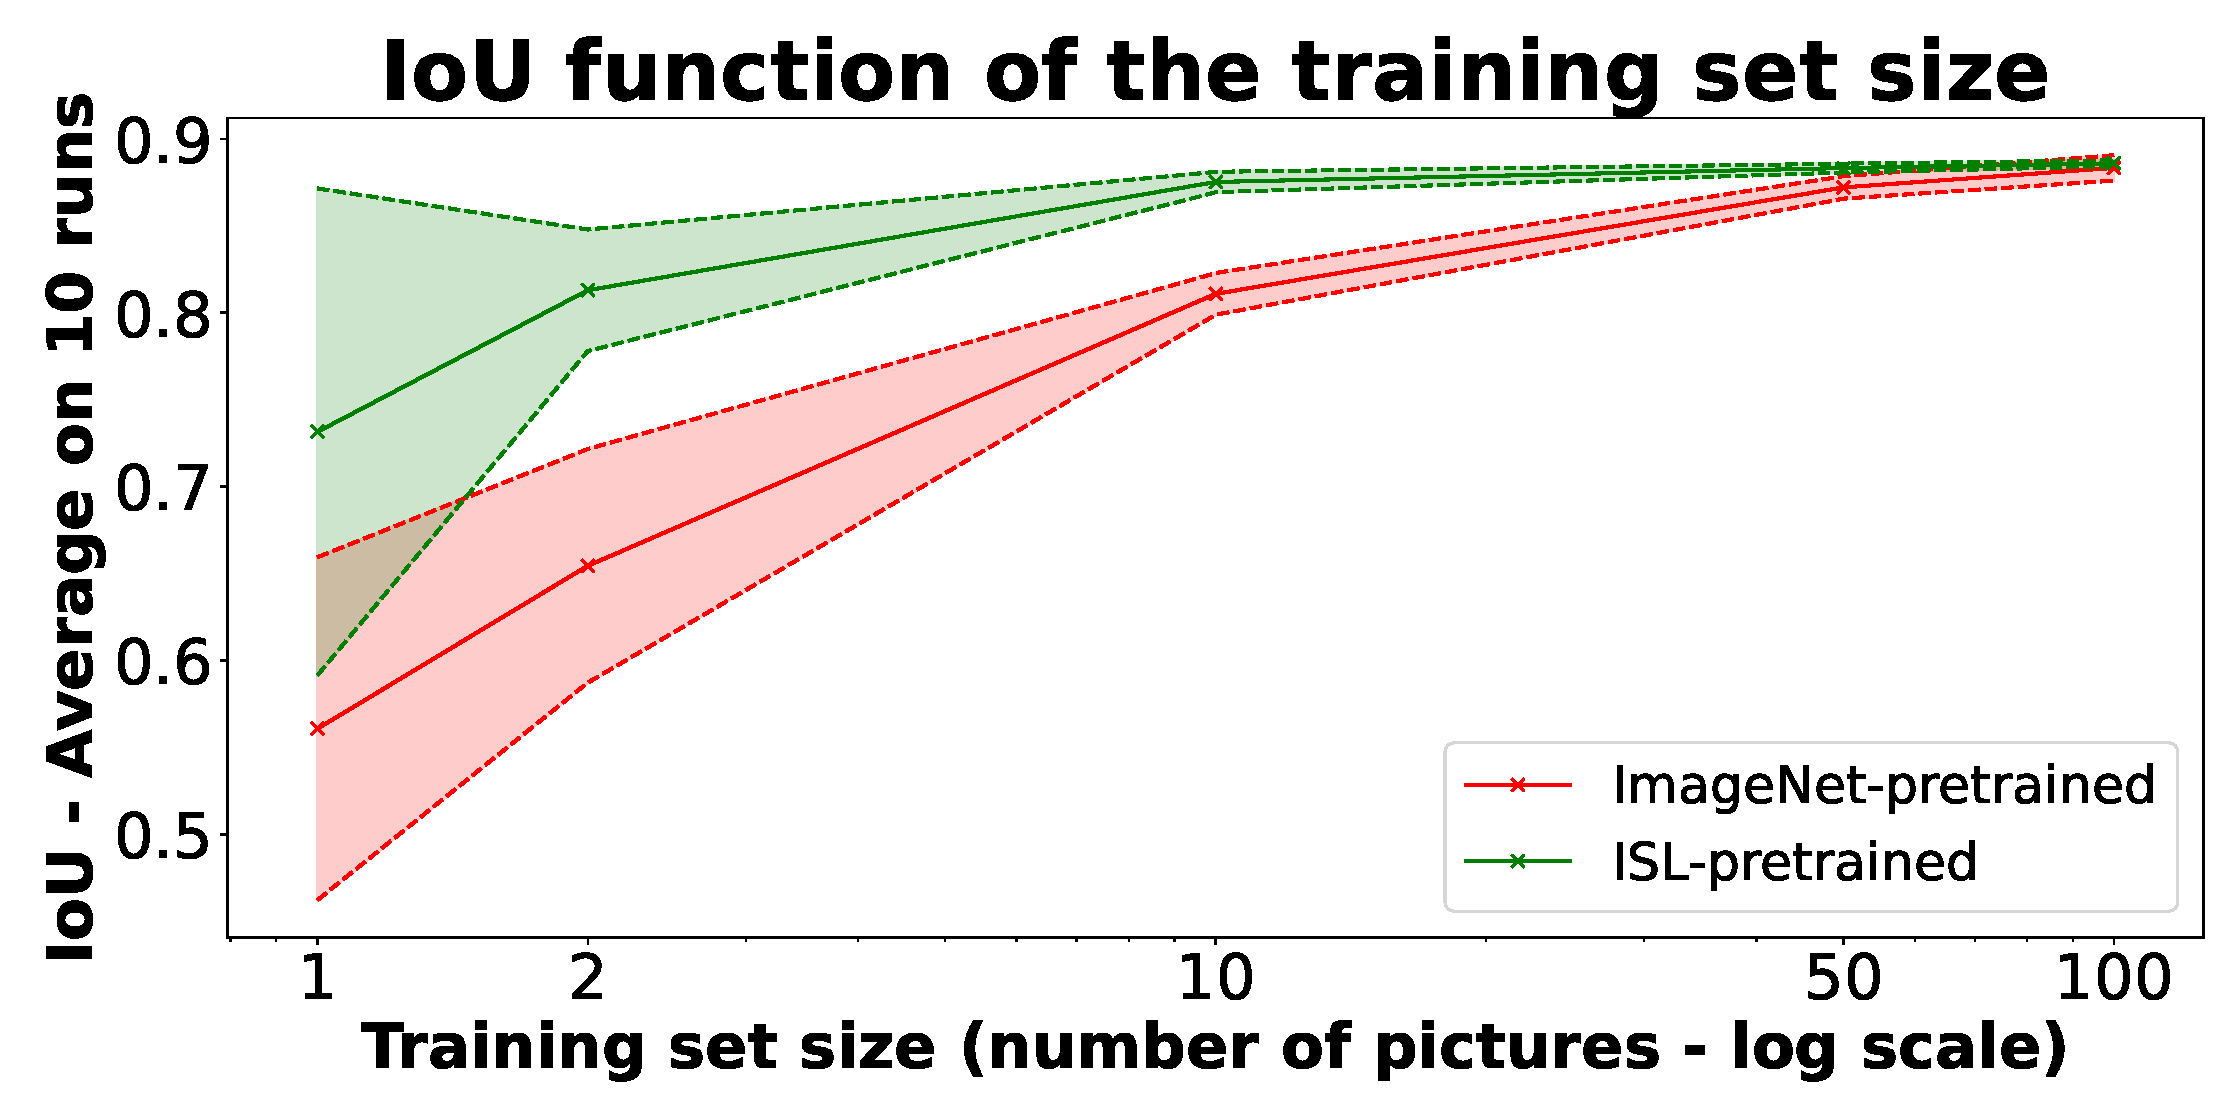
\includegraphics[width=\textwidth]{figures/chapter3/insilico_training_size}
    \caption[Results of in silico pre-training]{Results of in silico pre-training for a nucleus segmentation task, from~\cite{Bonte_2022}.
	IoU score for different training set size (the higher the better).
	Segmentation model with in silico pre-training (\textit{green}) is more efficient in low training dataset regime than model with ImageNet pre-training (\textit{red})}
    \label{fig:results_insilico}
\end{figure}

\section{Conclusion}
\label{sec:segmentation_conclusion}

This chapter details the different algorithms available in \emph{bigfish.segmentation} subpackage to segment nuclei and cells from fluorescent microscopy images.
The main interest of these methods is to propose in-house segmentation solutions, easy to use in few lines of code, and therefore complete the quantitative pipeline defined in FISH-quant.
Yet, the research community is quite dynamic concerning biomedical segmentation.
A lot of publications are released every year, with new datasets and improved techniques.
Beyond developing a potential state-of-the-art model (which would be surpassed a few months later), the ability to easily integrate results from external resources is essential for FISH-quant.
To this end, postprocessing methods are also implemented to format and refine segmentation masks.

Even if the segmentation has not been my main axis of research, I have explored some methods to alleviate limitations observed in cell segmentation.
During my PhD I have mainly worked with multichannel images considering both nuclei and cells.
For this reason, the consistency between nucleus and cell segmentation is critical.
Such consistency can be directly enforced by the way an algorithm works, like in a watershed transform, or learned through a specific training strategy.
Additionally, the need for a large amount of annotated images is still a hot topic in deep learning research.
The use of in silico techniques to pre-train models seems to mitigate this limitation. %
%%!TEX root = ../main.tex

\graphicspath{{./figures/chapter4/}}


\chapter{Spatial Feature Engineering}
\label{ch:chapter4}

\minitoc
\newpage

In this chapter we present and discuss different approaches to analyze \ac{RNA} localization patterns.
They require to quantify and measure indicators from fluorescent images.
To do so, we use a coordinate representation of cells, merging results from the detection~\ref{ch:chapter2} and segmentation~\ref{ch:chapter3} chapters.

We first present this representation, obtained with methods implemented in \emph{bigfish.multitask}.
In the second and third parts of this chapter we then present two different methods to compute spatial features.
We can manually design localization features or we can learn them, training a gradient-based pipeline on a pretext task.

The hand-crafted features are already implemented in \emph{bigfish.classification}.
The learned features section was mainly developed with the paper:

\begin{center}
	\color{green}
	Future paper to be released (ECCV workshop or arxiv)
\end{center}

\section{From images to coordinates}
\label{sec:image_coordinates}

We base our analysis on the coordinate representation of cells as illustrated in Figure~\ref{fig:cell_extracted_0}.
We exploit outcomes from detection and segmentation stages.
More precisely, for each individual cell we extract and identify coordinates of detected objects and segmentation masks.
As a reminder, current implementation in \emph{bigfish} allows a 2D or 3D detection, but only a 2D segmentation.
An extension to 3D segmentation masks is not planned, but could be easily implemented.
Any external methods for detection and segmentation could be used, as long as output formats match with \emph{bigfish} ones.

\begin{figure}[h]
    \centering
    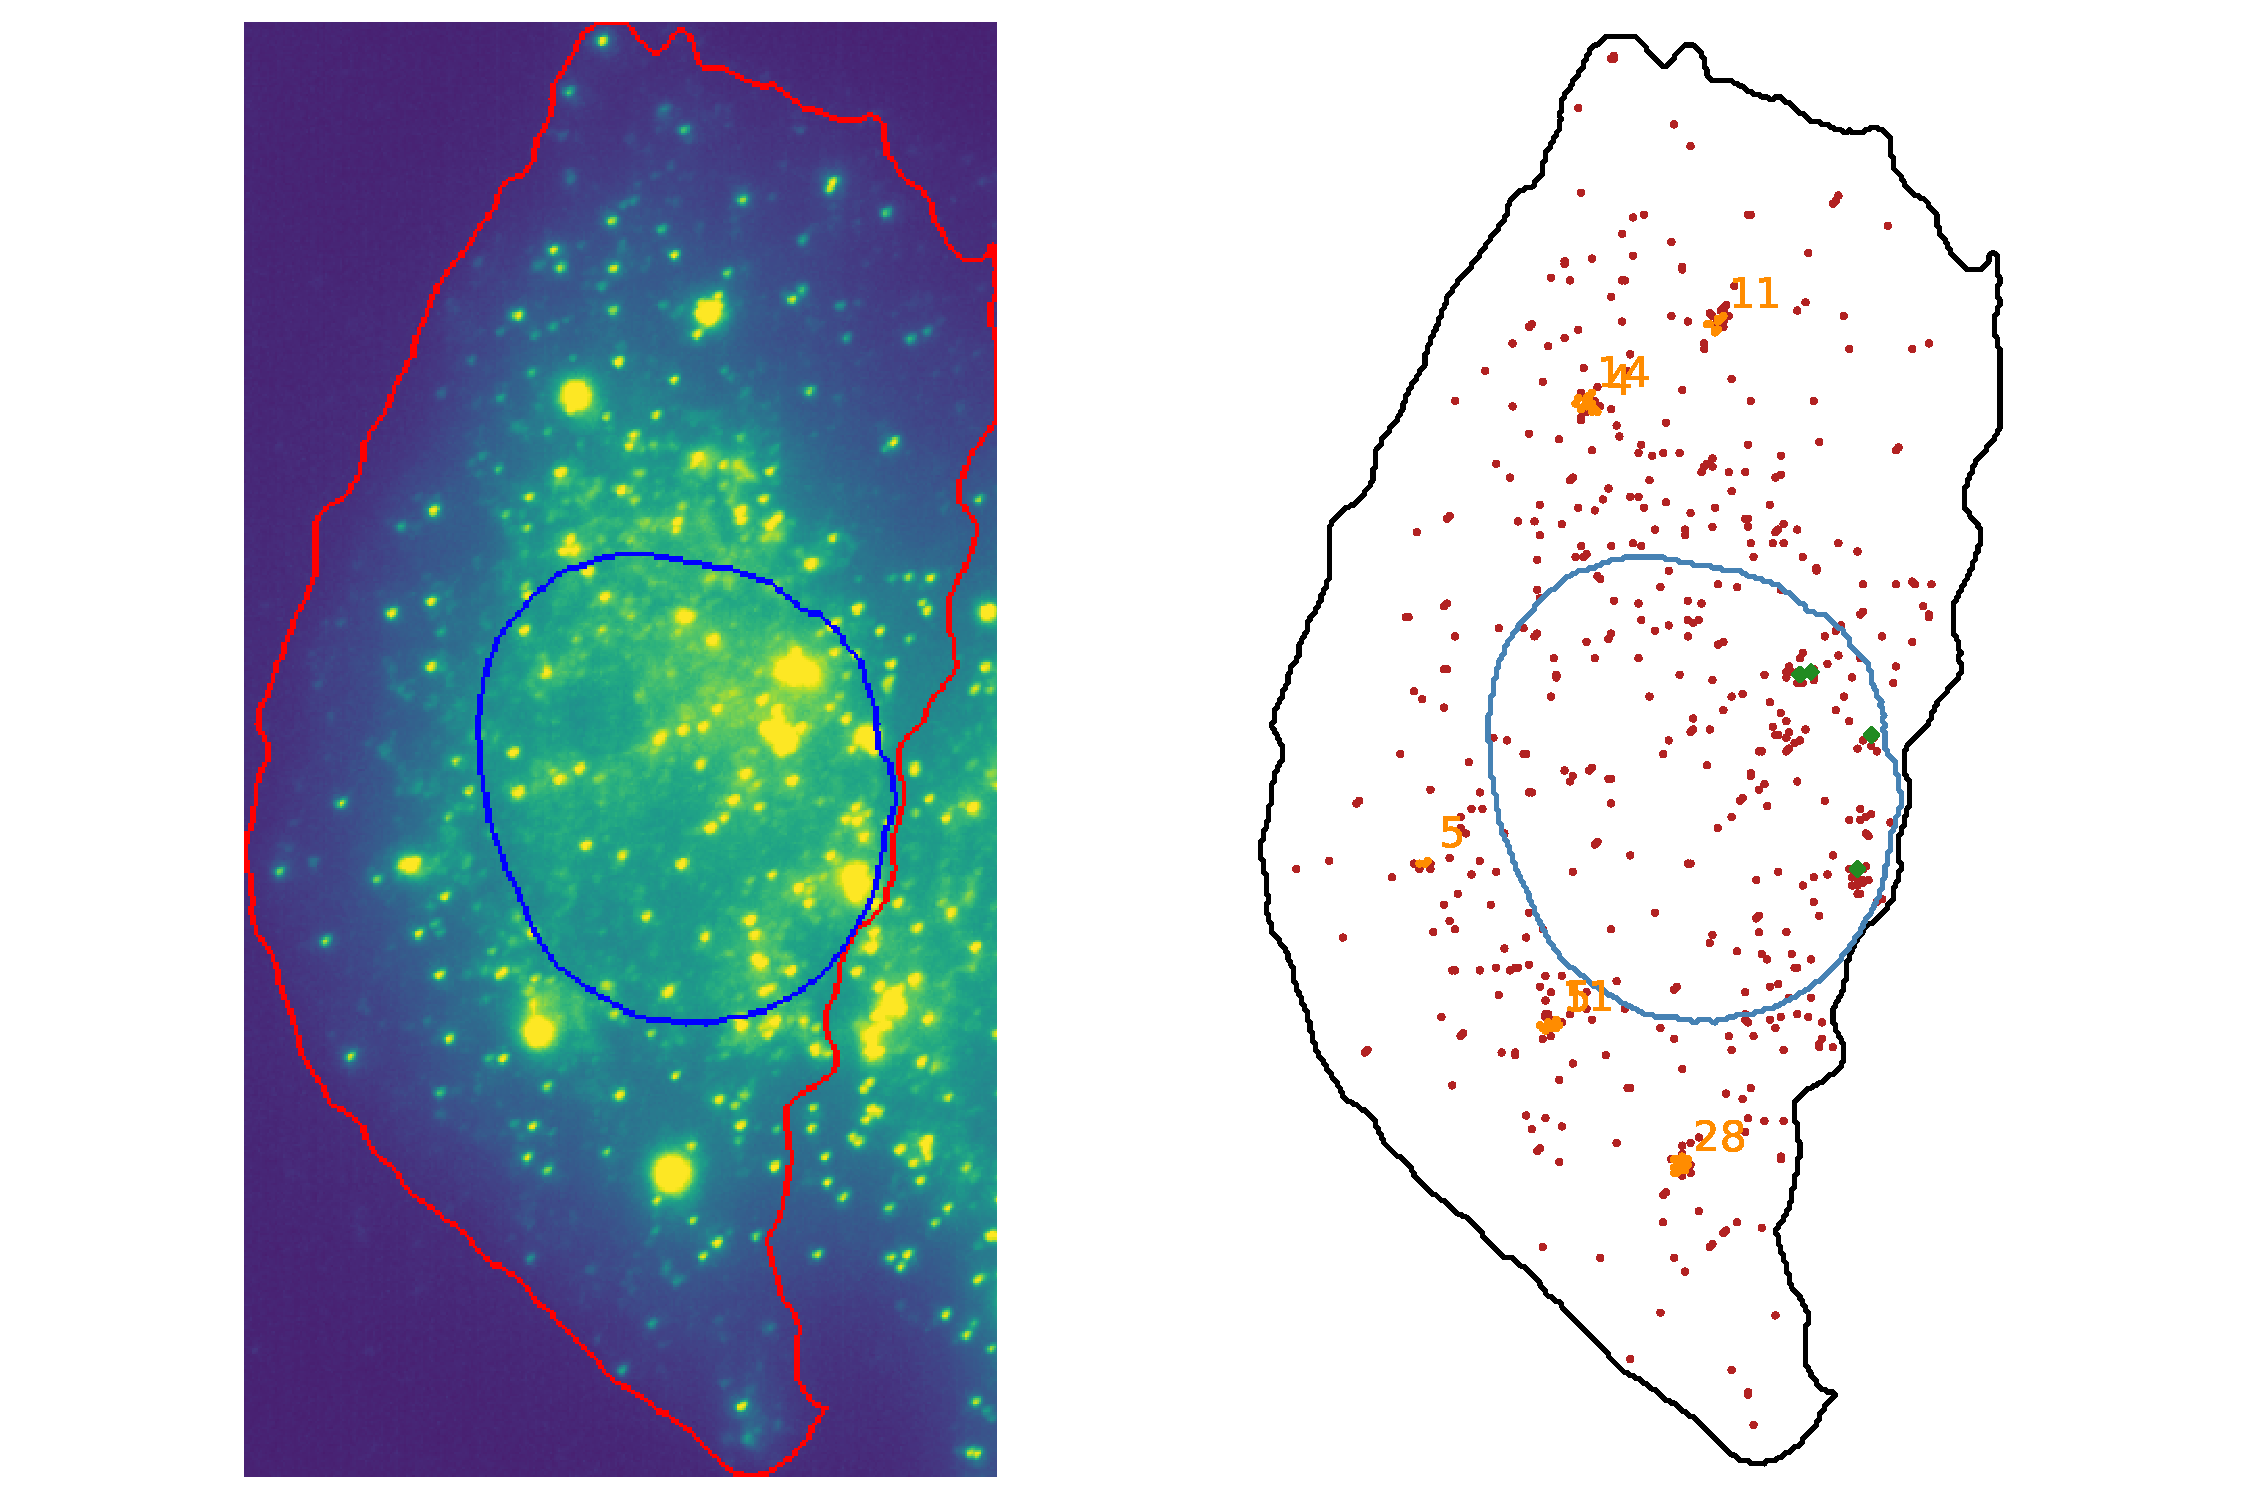
\includegraphics[width=\textwidth]{figures/chapter4/cell_extracted_0}
    \caption{Contrasted original image with segmented boundaries (\textit{left}) and coordinate representation (\textit{right}).
	Plot build with \emph{bigfish}}
    \label{fig:cell_extracted_0}
\end{figure}

\subsection{Object labelling}
\label{subsec:object_labelling}

In addition to detection and segmentation refinement, the possibility to merge results from both stages is highly valuable.
We can discriminate individual objects according to their localization in the cell.
A user might want to label a detected object if it locates within a segmented surface or not.
For example, some studies require to remove transcription sites before further analysis~\cite{CHOUAIB_2020}, or on the contrary to focus on them.
User could define a \ac{RNA} cluster inside nucleus as a transcription site, as opposed to the ones detected outside nucleus.
More generally, any detected object could be assigned to a specific cellular compartments, depending on the fluorescent labels available in the study.\\

% reference paper using transcription site only

\begin{minipage}{0.9\textwidth}
\begin{lstlisting}[language=Python]
import bigfish.multistack as multistack

# discriminate foci and transcription sites
spots_no_ts, foci, ts = multistack.remove_transcription_site(
	rna=spots,
	clusters=clusters,
	nuc_mask=nuc_label,
	ndim=3)
\end{lstlisting}
\end{minipage}

\subsection{Coordinate representation}
\label{subsec:coordinate_representation}

\subsubsection{Cell extraction}

To extract and summarize our \ac{FISH} results at the single cell level, the only requirement is a segmentation mask of the cell.
At least, user needs to perform instance segmentation to be able to identify individual cells.
Additional results are optional, but they greatly improve the quality of the information assigned to each cell.
Detected \ac{RNA} and cluster (or anything else detected) can be assigned to individual cells.
Nuclei segmentation masks make us able to delimitate nuclear membrane and define transcription sites or any nucleus-related object.
We can also crop input images around the identified cells, for every available channel.

In Figure~\ref{fig:cell_extracted_0} we can observe a cropped \ac{smFISH} image on the left, with cell and nuclear membranes in red and blue respectively.
On the right, these membranes are also visible (in black and blue respectively), in addition with \ac{RNA} spots (in red), \ac{RNA} clusters (in orange, with the estimated number of \ac{RNA} clustered) and transcription sites (in green).
With such \emph{extraction} we lose pixel-wise information like intensity values or image texture.
We also deeply rely on detection and segmentation performances to return meaningful coordinates.
Nonetheless, coordinate representation is a sparse and more natural representation for \ac{mRNA} localization pattern classification.
Indeed \ac{mRNA} molecules can be viewed as single point objects distributed in a 3D space.
Microscopic images with fluorescent labels are here the only medium we have to measure and approximate their localization, but still a medium.
ultimately, the original and relevant information is the 3D spatial coordinates of molecules we target.

Eventually we propose optional criteria to identify individual cells and refine the outcome.
First, we can ensure that only one nucleus is assigned to each cell.
Second, we can remove cropped cells at the border of the \ac{FoV}.
Their segmentation is incomplete and might bias final results.
Third, extracted cells can be filtered out according to the number of detected objects (especially the number of \ac{RNA}s).
By censoring empty cells, we remove potential outliers, detection or segmentation failures and therefore help a subsequent statistical analysis.\\

\begin{minipage}{0.9\textwidth}
\begin{lstlisting}[language=Python]
import bigfish.multistack as multistack

# extract cell-level results
fov_results = multistack.extract_cell(
    cell_label=cell_label,
    ndim=3,
    nuc_label=nuc_label,
    rna_coord=spots_no_ts,
    others_coord={"foci": foci, "transcription_site": ts},
    image=image_contrasted,
    others_image={"dapi": nuc_mip, "smfish": smfish_mip})
\end{lstlisting}
\end{minipage}

\subsubsection{Statistical description}

At this stage we can already compute standard, but useful statistics for every cell.
We measure cell and nucleus areas, but also \ac{RNA} distribution, inside and outside nucleus.
With cluster coordinates, estimation of cluster size is available, as well as proportion of clustered \ac{RNA}.
The \ac{RNA} proportion in specific cellular compartments are also noteworthy.
Such indicators are already relevant to quantify or validate meaningful biological insights.
For example, a recent study~\cite{cochard_rna_2022} uses \emph{bigfish} to estimate \ac{RNA} recruitment in bioengineered condensates (segmented from a \ac{GFP} channel).\\

\begin{minipage}{0.9\textwidth}
\begin{lstlisting}[language=Python]
import bigfish.multistack as multistack

# compute cell-level statistics
df = multistack.summarize_extraction_results(fov_results, ndim=3)
\end{lstlisting}
\end{minipage}

\section{Hand-crafted localization features}
\label{sec:hand_features}

We now present the first approach to analyze \ac{RNA} localization patterns in depth: we manually design spatial features.

\subsection{Related work}
\label{subsec:related_work_hand_features}

\subsubsection{Feature engineering with bioimages}

Bio-image computing field has long proposed quantitative frameworks and features to explore cellular mechanisms.
Some popular software includes complete analysis pipelines from image preprocessing to feature engineering.
For example CellProfiler~\cite{mcquin_cellprofiler_2018} allows researchers to count cell organelles and measure their size, analyze cell shape or extract pixel-wise texture information.
Expression level computation is also a standard, through proteome quantification.
CellCognition~\cite{held_cellcognition_2010} proposes a computational framework to annotate and classify relevant biological phenotypes, mostly through morphological measures.
More than 150 features are available.
Last but not least, ilastik~\cite{berg_ilastik_2019} also offers classification pipelines, with pixel-wise features such that intensity values, texture, brightness or color gradient.
Although useful and widely employed, these framework appear quickly limited for a \ac{smFISH} analysis which does not only rely on image texture or cell morphology.
More specialized libraries are needed.

\subsubsection{\ac{RNA} localization features}

Hand-crafted features to classify \ac{RNA} localization patterns were already developed in previous studies~\cite{battich_image-based_2013,samacoits_computational_2018}.
Generally such features are inspired by literature on spatial statistics~\cite{ripley2005spatial} and adapted for fluorescence microscopy images~\cite{lagache_statistical_2015,stueland_rdi_2019}.
Furthermore, several packages implement modules to perform \ac{smFISH} analysis and compute these hand-crafted features~\cite{mueller_fish-quant_2013,savulescu_dypfish_2019,mah_bento_2022}.

In~\cite{battich_image-based_2013}, authors designed 18 features ''that reflect the relative localization of each spot in a single cell, with respect to both the cell and other spots''.
They compute per-transcript features, then exploit their per-cell mean and standard deviation to identify subcellular localization patterns.
They even complete and extend their pipeline analysis in a subsequent work~\cite{stoeger_computer_2015}, by integrating segmentation and detection algorithms.

Two recent Python libraries greatly extend and facilitate the quantification of \ac{FISH} experiments.
DypFISH~\cite{savulescu_dypfish_2019} was developed to analyze \ac{RNA} and protein (co-)localization.
It includes features to investigate clustering and \ac{MTOC}-related patterns.
Across different imaging acquisitions of cells with a architecture constraints, they propose techniques to study \ac{mRNA}-protein spatial distribution~\cite{savulescu_interrogating_2021}.
Bento~\cite{mah_bento_2022} proposes modules to analyze images generated with \ac{SeqFISH} and \ac{MERFISH}.
They adapt feature extraction pipeline to highly multiplexed spatial transcriptomics data.

In the first FISH-quant version~\cite{mueller_fish-quant_2013} more than 20 features are implemented in MATLAB.
They are extensively evaluated in a recent publication~\cite{samacoits_computational_2018} with simulated localization patterns.
Compared to previous features developed in the literature~\cite{battich_image-based_2013}, they return a better performance to classify \ac{RNA} localization patterns.
A first set of features includes distance features between \ac{RNA} spots and cell or nucleus.
A second set of features involved the Ripley K-function~\cite{ripley2005spatial}:

\begin{equation}
	{\displaystyle K(r) = \frac{1}{n} \sum_{i = 1}^{n} \frac{N_i(r)}{\lambda}}
\end{equation}

\noindent
With $N_i$ Npi (r) the number of \ac{RNA}s in a circle of radius $r$ centered on the $i^{th}$ \ac{RNA} and $\lambda$ the total density of \ac{RNA}s in the cell
It quantifies the aggregation or dispersion of mRNAs
Several features are designed from these values, exploiting their maximum or their correlation with the radius $r$.
However, Ripley features are sensitive to boundary effects (\ac{RNA}s close to a membrane have a limited neighborhood) and require to be correctly normalized.
A third set of features is based on morphological operations, like opening, to identify cell extensions.
Lastly, dispersion and polarization indices are implemented.
Some of our own hand-crafted features are implementations or improvements of this work.

\subsection{Expert features}
\label{subsec:expert_features}

A large part of hand-crafted features we implemented in \emph{bigfish.classification} were initially designed for our own studies~\cite{CHOUAIB_2020,safieddine_choreography_2021,pichon_kinesin_2021}.
These features capture more specific information about \ac{RNA} localization, beyond surface areas (\emph{cell\_area} and \emph{nuc\_area}) or expression levels (\emph{nb\_rna}).

\subsubsection{Distance features}

We first reuse and adapt some distance features already implemented in the first FISH-quant version and presented in a recent paper~\cite{samacoits_computational_2018}.
Distances from cell or nuclear membranes are computed in 2D as we only use 2D segmentation results so far.
However, such features could be easily extended with 3D segmentation masks.
We compute the average distance between detected \ac{RNA}s and cell membrane \emph{index\_mean\_distance\_cell} such that:

\begin{equation}
	{\displaystyle \operatorname{index\_mean\_distance\_cell} = \frac{\overline{d_{cell}(x_i, y_i)}}{\lambda_{cell}}}
\end{equation}

\noindent
With $d_{cell}(x_i, y_i)$ the euclidean distance to the cell membrane for the rna $i$ and $\lambda_{cell}$ the expected average distance under uniform \ac{RNA} distribution.
A previous study~\cite{battich_control_2015} used the square root of cell area to normalize its distance features.
However, as noticed by~\cite{samacoits_computational_2018}, it does not take into account a potential heterogeneity in terms of cell morphology.
For this reason we approximate $\lambda_{cell}$ as the average value of the 2D distance map from the cell membrane.
Similarly, we compute the normalized average distance of \ac{RNA}s to the nucleus: \emph{index\_mean\_distance\_nuc}.
Alternative computation with the median function is available for these two features too.

Unlike the first FISH-quant version, we do not compute distances to cell or nucleus centroids, nor quantiles of the \ac{RNA} distance distribution.
These features might appear redundant to quantify distance information.

\subsubsection{Morphological features}

A second set of features is related to the localization of \ac{RNA} in specific cell compartments.
We already count the number of transcripts detected inside the nucleus.
More precisely, proportion of \ac{RNA}s inside the nucleus (\emph{proportion\_rna\_in\_nuc}) is a good enough indicator to identify intranuclear pattern.

\begin{figure}[h]
    \centering
    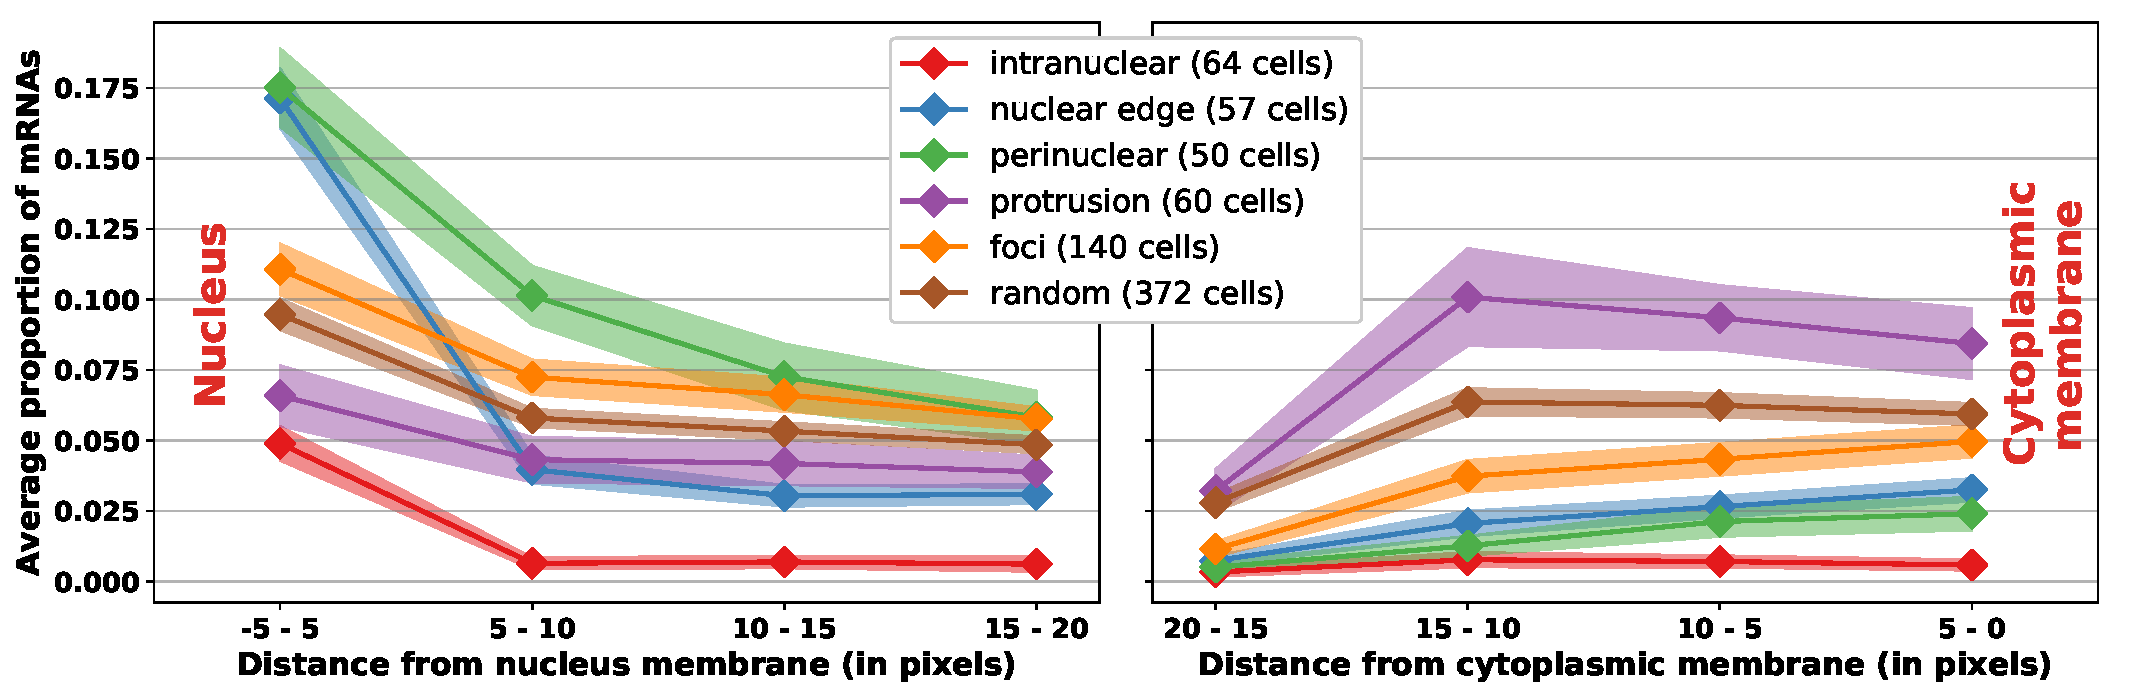
\includegraphics[width=\textwidth]{figures/chapter4/plot_topography}
    \caption{Proportion of mRNA at various distances from cell and nuclear membranes.
	Dataset and annotated patterns from~\cite{CHOUAIB_2020}.
	\textit{Colored areas} represent the 95\% confidence interval}
    \label{fig:features_topography}
\end{figure}

Still we can go further to partition cell regions.
We define a list of features to measure the distribution of \ac{RNA}s within different cell regions.
Regions of interest are delimited with concentric circles from cell or nuclear membranes, with an interval distance of 500nm each.
More precisely, area between 0 and 3000nm from the cell membrane is divided in six concentric regions.
In each region we compute \ac{RNA} proportion (\emph{proportion\_rna\_cell\_radius\_1000\_1500} for the proportion between 1000nm and 1500nm from the cell membrane) or we count the number of \ac{RNA}s we detect, normalized by the expected number of \ac{RNA}s under random distribution (\emph{index\_rna\_cell\_radius\_1000\_1500}).
We also define 5 more regions around the nuclear membrane between 500nm and 3000nm.
Another region is defined along the nuclear membrane, including detected \ac{RNA}s inside or outside the nucleus, but within 500nm from its membrane.
Likewise, proportion (\emph{proportion\_rna\_nuc\_radius\_500\_1000}) and normalized \ac{RNA} count (\emph{index\_rna\_nuc\_radius\_500\_1000}) are computed for all regions around the nuclear membrane.
When we manually annotate real cells and identify different localization pattern we measure how discriminative these features can be.
In Figure~\ref{fig:features_topography} we observe average \ac{RNA} proportion for the different regions we described.
The 95\% confidence interval is also reported in the plot.
Logically, nuclear edge and perinuclear patterns present a higher proportion of \ac{RNA} along the nuclear membrane.
On the opposite, cells with a protrusion pattern have a higher \ac{RNA} density along the cell membrane.

We focus on a last relevant region in a cell: protrusions.
To design features related to cell extension we first need to define such extension.
Like~\cite{samacoits_computational_2018} we define this region as the lost area after applying a morphological opening (an erosion followed by a dilation) to the cell mask.
For this operation we use a disk with 3000nm radius as a structuring element.
We then compute the proportion of \ac{RNA} (\emph{proportion\_rna\_protrusion}) or the normalized \ac{RNA} count (\emph{index\_rna\_protrusion}) in protrusion.

\subsubsection{Dispersion features}

We implement three features described and tested in a recent paper~\cite{stueland_rdi_2019} to quantify \ac{RNA} polarization and dispersion within the cell.

Polarization index is computed by comparing \ac{RNA} point cloud centroid and cell centroid:

\begin{equation}
	{\displaystyle \operatorname{index\_polarization} = \frac{\sqrt{(x_{rna} - x_{cell})^2 + (y_{rna} - y_{cell})^2}}{Rg_{cell}}}
\end{equation}

\noindent
With $(x_{rna}, y_{rna})$ the coordinates of the \ac{RNA} centroid and $(x_{cell}, y_{cell})$ the coordinates of the cell centroid.
The radius of gyration $Rg_{cell}$ normalizes the index for different cell sizes.
It is defined as the root-mean-squared distance between every cell pixel and the cell centroid.
The higher, the more polarized \ac{RNA}s are.

Dispersion index measures the dispersion of the \ac{RNA} point cloud.
In addition to the extracted coordinates, its computation also implies pixel intensities from the original \ac{smFISH} image:

\begin{equation}
	{\displaystyle \operatorname{index\_dispersion} = \frac{\frac{\sum_{i} r_i^2 I_i}{\sum_{i} I_i}}{\frac{\sum_{j} r_j^2 I_j}{\sum_{j} I_j}}}
\end{equation}

\noindent
With $r_i$ and $r_j$ the euclidean distance of \ac{RNA} $i$ and cell pixel $j$ to the \ac{RNA} centroid respectively, $I_i$ the pixel intensity of \ac{RNA} $i$ and $I_j$ the pixel intensity of cell pixel $j$.
Pixel intensity of transcripts distant from the \ac{RNA} centroid are overweighted.
As the index is normalized considering every pixel $j$ from the cell mask, it tends to 1 when \ac{RNA} point cloud is uniformly distributed.
A diffuse point cloud has a value greater than 1.
On the opposite, if \ac{RNA}s are concentrated anywhere in the cell, index value is lower than 1.

Peripheral distribution index measures how close the \ac{RNA}s localize to the cell periphery (\emph{index\_peripheral\_distribution}).
Its computation is similar to the dispersion index, but the \ac{RNA} centroid is replaced by the nucleus one in the equation.
A completely dispersed point cloud still has a value of 1, but it increases if \ac{RNA}s move toward the cell periphery, with a concentrated or diffused pattern.
Again, an aggregation of transcripts around the nucleus centroid (often close to the cell centroid too) decreases index value.

\subsubsection{Centrosomal features}

\begin{wrapfigure}{R}{0.40\textwidth}
	\begin{center}
	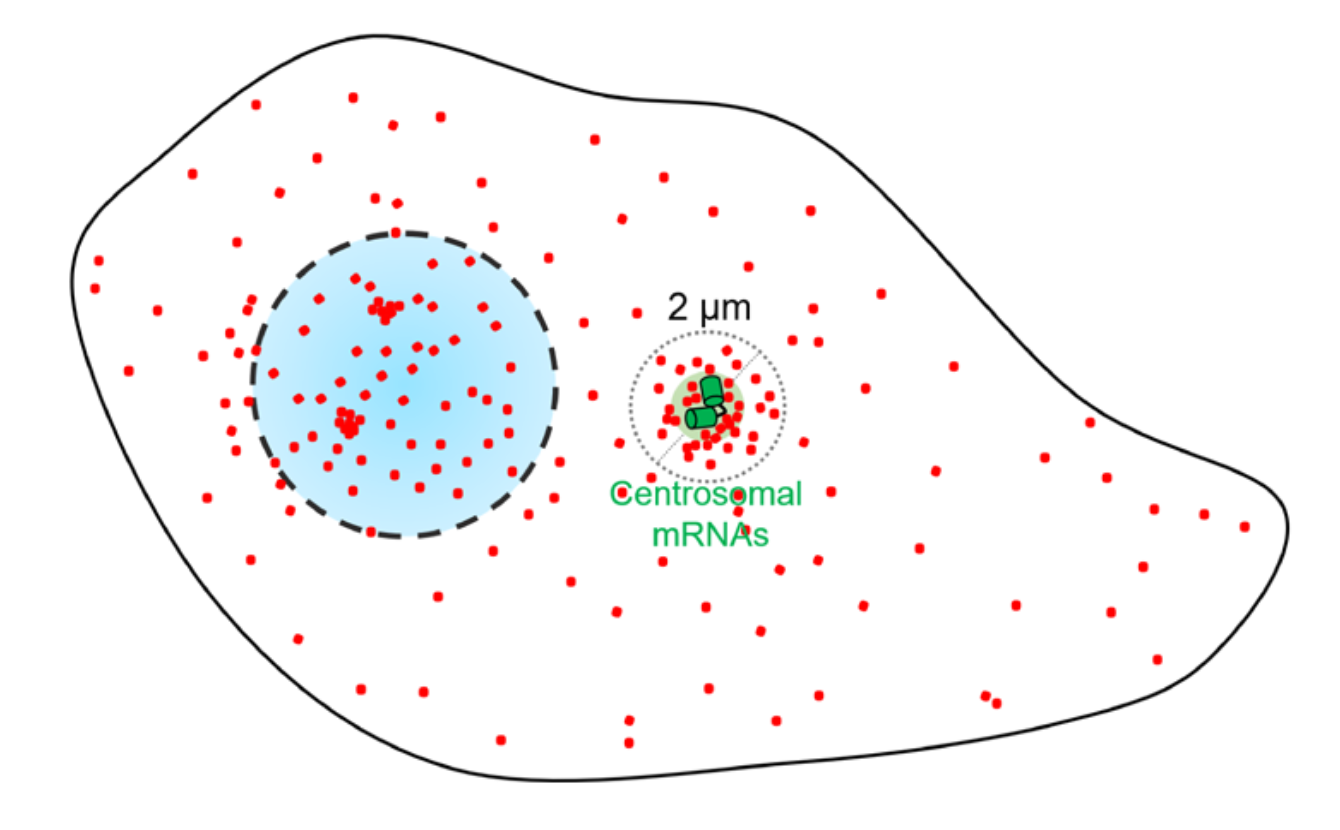
\includegraphics[width=\linewidth]{figures/chapter4/centrosomal_features}
	\caption{Centrosomal RNAs and its neighborhood from~\cite{safieddine_choreography_2021}}
	\label{fig:centrosome_features}
	\end{center}
\end{wrapfigure}

If we detect additional object and extract new coordinates besides individual and clustered \ac{RNA}s, more specific features can be designed.
For example, these objects can be cell organelles labelled during the experimentation.
We design such features with the centrosomes to further study \ac{RNA} localization related to the \ac{MTOC}~\cite{safieddine_choreography_2021}.

A first obvious feature is the average (or median) distance between \ac{RNA}s and the closest detected centrosomes (up to two centrosomes can be detected in the cell): \emph{index\_mean\_distance\_centrosome}.
Similarly to the distance features we compute with the cell or nuclear membranes, we compute the expected distance under uniform \ac{RNA} distribution for normalization.

A second set of features consists in delimiting an area around each centrome to be considered as centrosome's neighborhood.
In our case we manually choose a radius of 2000nm around centrosomes to define such areas, as illustrated in Figure~\ref{fig:centrosome_features}.
We can then compute the normalized \ac{RNA} count (\emph{index\_rna\_centrosome}) or the \ac{RNA} proportion (\emph{proportion\_rna\_centrosome}) in these regions.

Lastly, we derived a feature from the dispersion index described above.
We define a centrosomal dispersion index to quantify \ac{RNA} dispersion around centrosomes: \emph{index\_centrosome\_dispersion}.
We design it like the dispersion index, but instead of \ac{RNA} centroid, we use the closest centrosome coordinates to compute the euclidean distance.
The lower, the closer \ac{RNA}s localized to the centrosomes.

\subsubsection{Cluster features}

Concerning cluster localization patterns, we observed than our clustering method (see subsection~\ref{subsec:dense_decomposition}) already captures good enough information.
More specifically, number of detected clusters (\emph{nb\_foci}) or \ac{RNA} proportion inside these clusters (\emph{proportion\_rna\_in\_foci}) are relevant features to identify transcripts with a tendency for clustering.
As a consequence, and unlike~\cite{samacoits_computational_2018}, we do not implement diverse features based on the famous Ripley's K-function.
This would require tuning a lot more parameters than just reusing the detected number of clusters.\\

\begin{minipage}{0.9\textwidth}
\begin{lstlisting}[language=Python]
import bigfish.classification as classification

# compute features
features, features_names = classification.compute_features(
    cell_mask=cell_mask,  # individual cell mask
	nuc_mask=nuc_mask,  # individual nucleus mask
	ndim=3,
	rna_coord=rna_coord,
    smfish=smfish,
	voxel_size_yx=103,  # in nanometer
    foci_coord=foci_coord,
    compute_distance=True,
    compute_intranuclear=True,
    compute_protrusion=True,
    compute_dispersion=True,
    compute_topography=True,
    compute_foci=True,
    compute_area=True,
    return_names=True)
\end{lstlisting}
\end{minipage}

\section{Learned localization features}
\label{sec:learned_features}

A second approach to analyze \ac{RNA} localization patterns is to learn features.
To this end we design and train a deep learning model, PointFISH, on a simulated pretext task.
We then reuse the internal representation learned by the model as a point cloud embedding to discriminate \ac{RNA} localization patterns.
The later is evaluate on an experimental dataset.

\subsection{Related work}
\label{subsec:related_work_learned_features}

\subsubsection{Learning features and embeddings}

A neural network learns representations that we can use for transfer learning.
One advantage is to pretrained relevant representations on a first task with a large and general annotated dataset, before addressing a more difficult or specific task with sometimes a limited dataset available.
Such model can be used as a feature extractor by computing features from one of its intermediate layers.
Computer vision community progressively replaces hand-crafted features~\cite{Lowe_1999,Bay_2006} by deep learning features to analyze images.
Best convolutional neural networks pretrained on large and general classification challenges~\cite{He_2016_CVPR,Szegedy_2016_CVPR,Tan_2019,Huang_2017_CVPR} are used as backbone or feature extractor for more complex task like face recognition, detection or segmentation.
NLP community follows this trend as well with a heavy use of word embeddings~\cite{Mikolov_2013,Joulin_2016} or the more recent transformers models.
As a last example, with graph computation, node2vec~\cite{Grover_2016} learns ''task-independent representations'' for nodes in networks.

Such embedding has also the advantage to be a continuous and numerical representation.
This is especially useful when dealing with a non-structured data like text or graph.
With spage2vec~\cite{Partel_2021}, authors learn a low dimensional embedding of local spatial gene expression (expressed as graphs).
Eventually, they identify meaningful gene expression signatures by computing this embedding for tissue datasets.

\subsubsection{Convolutional features}

Because we analyze smFISH images, a first intuition would be to build a convolutional neural network to directly classify localization patterns from the fluorescent image.
This approach is actually already in place for protein localization.
Unlike RNA, proteins are usually studied with Green fluorescent protein (GFP) markers and are difficult to resolve individually.
In this case, they appear as a gradient of intensity in the fluorescent image and thus protein localization has often been approached like texture classification problem.
First studies~\cite{boland_automated_1998} for example compute a set of feature from the microscopy image before training a classifier.
With recent successes of deep learning, protein localization is now tackled with convolutional neural network, but still framed as a texture classification problem.
After crowdsourcing annotations for the Human Protein Atlas dataset~\cite{Uhlen_2015} (through a video game), researchers trained a machine learning model (Loc-CAT) from hand-crafted features to predict subcellular localization patterns of proteins~\cite{sullivan_deep_2018}.
In a second time, they organized an online challenge~\cite{ouyang_analysis_2019} where a majority of top-ranking solutions were based on convolutional neural networks.
For protein localization the shift from hand-crafted features to convolutional features is significant and allows more accurate and robust pipelines.

A recent perspective paper~\cite{Savulescu_2021} foster the use of deep learning models for RNA localization analysis.
Today, such analysis can be performed with fluorescent images or RNA sequencing.
Authors emphasize the recent successes and flexibility of neural nets with both types of input, and therefore the possibility to design a multimodal pipeline.
However, smFISH images have clear spots that can be individually resolved and easily detected.
Therefore, a texture classification approach seems suboptimal to address \ac{RNA} localization pattern recognition.

% references CNN for biological images
% Moen, E. et al. Deep learning for cellular image analysis. Nat. Methods https://doi.org/10.1038/s41592-019-0403-1 (2019).
% Godinez, W. J., Hossain, I., Lazic, S. E., Davies, J. W. & Zhang, X. A multi-scale convolutional neural network for phenotyping high-content cellular images. Bioinforma. Oxf. Engl. 33, 2010–2019 (2017).
% Hofmarcher, M., Rumetshofer, E., Clevert, D.-A., Hochreiter, S. & Klambauer, G. accurate prediction of biological assays with high-throughput microscopy images and convolutional networks. J. Chem. Inf. Model. 59, 1163–1171 (2019).
% Kraus, O. Z., Ba, J. L. & Frey, B. J. Classifying and segmenting microscopy images with deep multiple instance learning. Bioinformatics 32, i52–i59 (2016).

\subsubsection{Point cloud models}

We postulate that learning to classify RNA localization patterns directly from detected spots coordinates is the most efficient approach.
A point cloud has an unordered and irregular structure.
Projecting the coordinates into images or voxels~\cite{Maturana_2015} transforms the problem as an easier vision challenge, but it comes along with some input degradations.
It dramatically increases the memory needed to process the sample and loses relevant spatial information.
In case of \ac{RNA} point cloud, we have already explored this approach by using convolutional neural network on a binary image of the point cloud~\cite{dubois_deep_2019}.
It makes the recognition of 3D localization patterns harder~\cite{dubois_deep_2019}.
A more detailed description of the method is available in appendix~\ref{ch:convolutional_features}.

A recent paper~\cite{khater_caveolae_2019} proposes to train a machine learning pipeline to discriminate caveolae clusters from scaffolds clusters.
These cell structures can be recognized through the detection of caveolin-1 proteins and the shape of the resulting point clouds acquired from \ac{SMLM} techniques.
Authors compare three pipelines to address the problem: a random forest classifier trained on hand-crafted features, a convolutional neural network applied on the point cloud image and more importantly a PointNet fed directly with point cloud.
Albeit legitimate, the PointNet method is less successful for this task than the two others pipelines.
Possibly, this model is too naive.

PointNet~\cite{Qi_2017_CVPR} is a seminal work that leads the way for innovative models to address shape classification.
It directly processes point clouds with share MLPs and a max pooling layer, making the network invariant to input permutation.
However, the pooling step is the only way for the model to share information between close points, which ultimately limits its performance.
Yet, recent research dramatically improves point cloud modelling and especially the capture of local information.

PointNet++~\cite{Qi_2017} learns local geometric structures by recursively apply PointNet to different regions of the point cloud, in a hierarchical manner.
This way, local information can be conveyed through the network more efficiently.
DGCNN~\cite{Wang_2019} proposes a new EdgeConv layer where edge features are computed between a point and its neighbors.
Some models propose to adapt convolutions to point cloud by designing new weighting functions or kernel operations like PointCNN~\cite{Li_2018}, PointConv~\cite{Wu_2019_CVPR} or KPConv~\cite{Thomas_2019_ICCV}.
Another inspiration from the computer vision or NLP literature is the attention-based model.
To this end, PointTransformer~\cite{Zhao_2021_ICCV} proposes an attention layer to be applied to local regions within the point cloud.
Last but not least, PointMLP~\cite{ma2022rethinking} proposes a simple but still efficient network with a pure deep hierarchical MLP architecture.

\subsection{Problem statement}
\label{subsec:problem_statement}

We want to train a model, where we can provide directly the point cloud coordinates as an input and compute a continuous vector representation.
This representation can then be used for classification of different \ac{RNA} localization patterns.
Such a deep learning model might require a large volume of annotated data to reach a satisfying performance.
To generate such a large data sets, we used simulated data to train our point cloud model and then use it as a trained feature extractor.
Eventually we evaluate these learned features on a experimental dataset.

\begin{figure}[h]
	\centering
	\minipage{0.33\textwidth}
		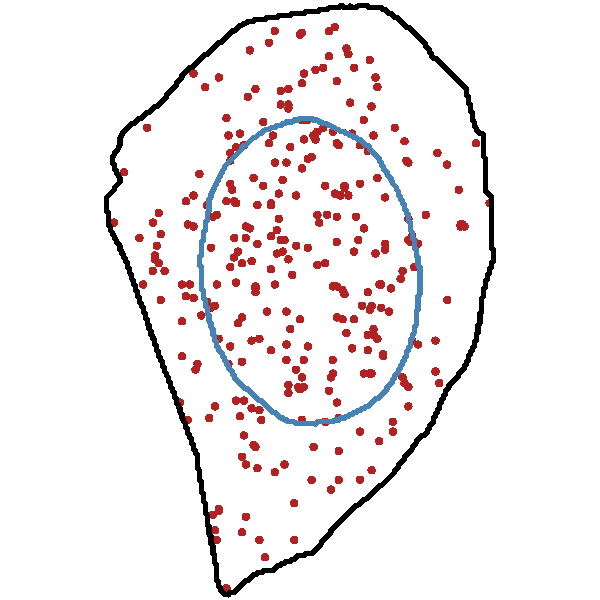
\includegraphics[width=\linewidth]{figures/chapter4/simulation_foci_10}
		\subcaption{10\% clustered RNA}
	\endminipage\hfill
	\minipage{0.33\textwidth}
		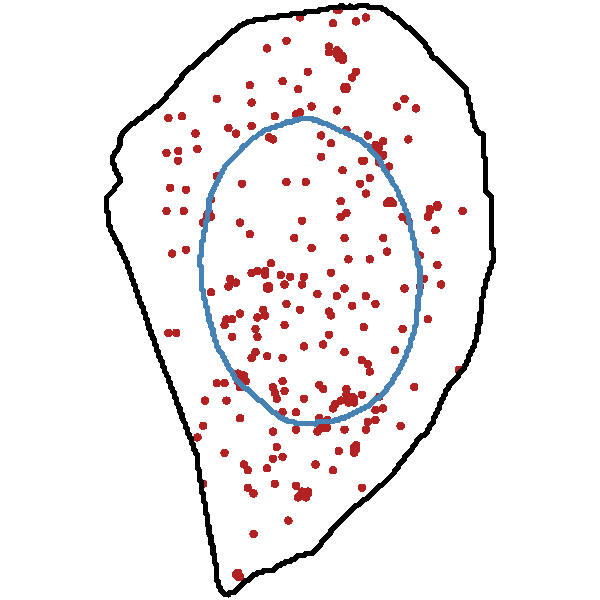
\includegraphics[width=\linewidth]{figures/chapter4/simulation_foci_50}
		\subcaption{50\% clustered RNA}
	\endminipage\hfill
	\minipage{0.33\textwidth}
		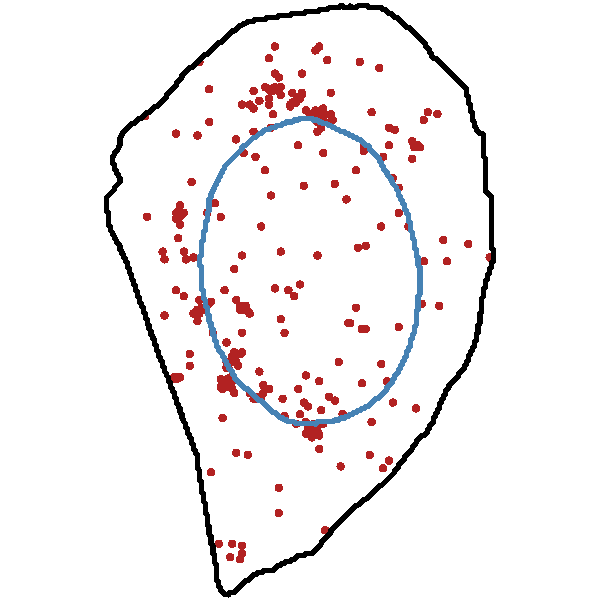
\includegraphics[width=\linewidth]{figures/chapter4/simulation_foci_90}
		\subcaption{90\% clustered RNA}
	\endminipage
	\caption{Foci pattern with increasing pattern strength simulated with \emph{simfish}}
	\label{fig:foci_panel}
\end{figure}

\subsubsection{Localization pattern simulations}

To build our simulated dataset, we use methods implemented in \emph{simfish}.
Our package exploits a template of 318 real cells to simulate realistic point clouds.
They were originally extracted for the first version of FISH-quant~\cite{samacoits_computational_2018} to simulate realistic cell and nucleus shapes.
We have the 3D segmentation masks for the cell and the nucleus.
In addition, we have manual annotations about potential protrusions, in case we want to simulate this specific pattern.
Several improvements are brought by \emph{simfish}:
\begin{itemize}
	\item We migrate to Python and do not rely on a proprietary framework anymore.
	\item We accelerate the simulation process.
	\item We extend the number of localization patterns available.
	\item We make simulations more consistent in terms of pattern strength.
\end{itemize}

Simulation's outcome includes the cell mask and its membrane coordinates (in 2D), the nucleus mask and its membrane coordinates (in 2D) and the \ac{RNA} coordinates (in 3D).
To match with the rest of the \emph{bigfish} pipeline, we voluntarily return 2D membrane coordinates.
A first parameter to set is the number of \ac{RNA}s $n$ we want to simulate.
To modulate the pattern strength, we set the proportion of \ac{RNA}s $p$ with a biased localization we want.
For example to simulate pattern with a moderate strength, we can simulate between 30\% and 50\% of the \ac{RNA} with the targeted localization bias, and the rest uniformly across the cell.
Lastly, we choose a pattern to simulate.

\begin{figure}[h]
	\centering
	\minipage{0.33\textwidth}
		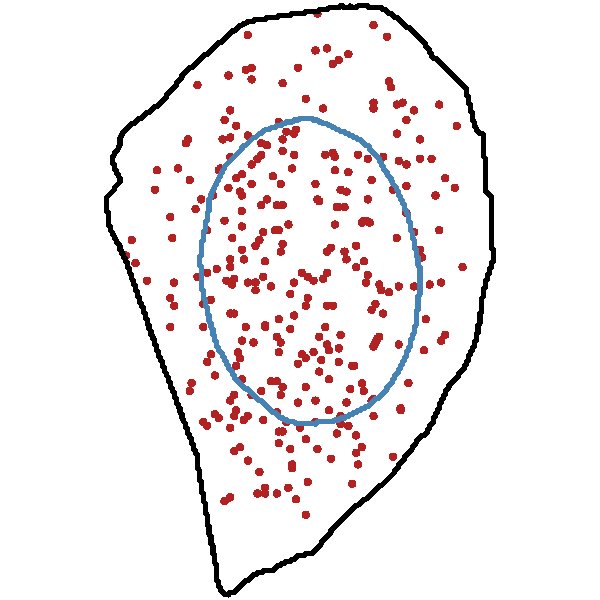
\includegraphics[width=\linewidth]{figures/chapter4/simulation_perinuclear_10}
		\subcaption{10\% perinuclear RNA}
	\endminipage\hfill
	\minipage{0.33\textwidth}
		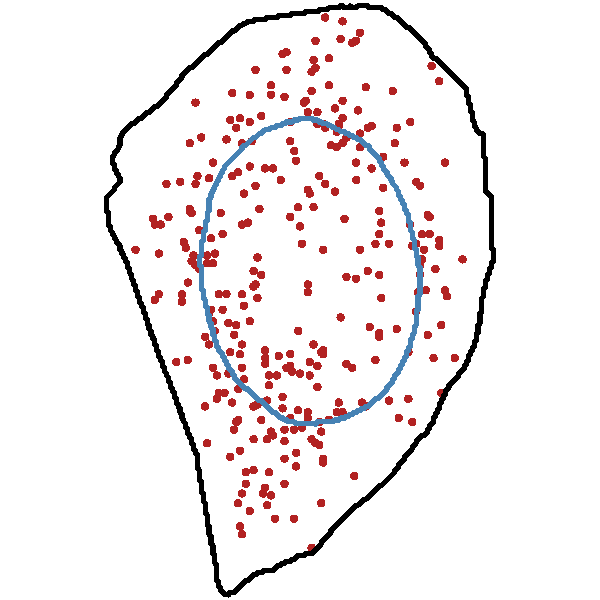
\includegraphics[width=\linewidth]{figures/chapter4/simulation_perinuclear_50}
		\subcaption{50\% perinuclear RNA}
	\endminipage\hfill
	\minipage{0.33\textwidth}
		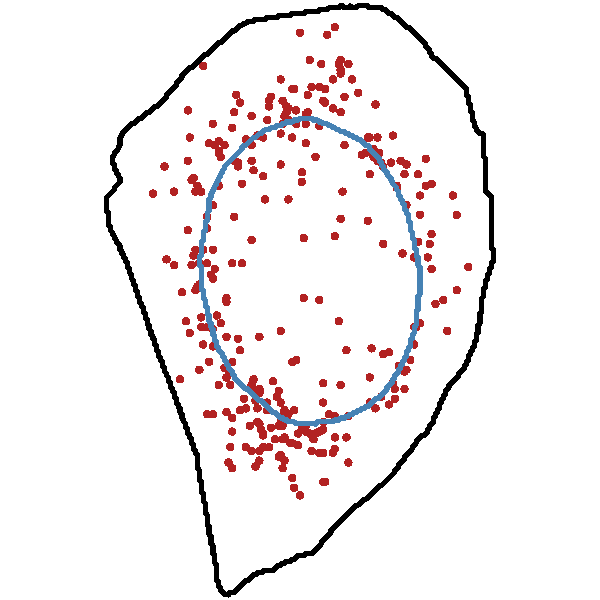
\includegraphics[width=\linewidth]{figures/chapter4/simulation_perinuclear_90}
		\subcaption{90\% perinuclear RNA}
	\endminipage
	\caption{Perinuclear pattern with increasing pattern strength simulated with \emph{simfish}}
	\label{fig:perinuclear_panel}
\end{figure}

The 9 patterns currently available are: random, foci, intranuclear, extranuclear, nuclear edge, perinuclear, cell edge, pericellular and protrusion.
Random pattern is the default pattern where \ac{RNA}s are simulated uniformly within the cell.
Foci pattern consists in a random number of \ac{RNA} clusters localizing outside the nucleus.
More precisely, we compute the total number of clustered \ac{RNA}s as $n_{pattern} = n \times p$.
We draw the expected number of \ac{RNA}s $\lambda$ per cluster from an uniform distribution between 5 and 21 \ac{RNA}s.
The number of clusters itself results from $n_{cluster}= \frac{n_{pattern}}{\lambda}$.
For each cluster, a distinct number of \ac{RNA}s is draw again with a Poisson distribution of mean $\lambda$.
Clusters are then localized outside the nucleus and remaining \ac{RNA}s uniformly in the cell.
In Figure~\ref{fig:foci_panel} we can observe foci simulations with an increasing pattern strength (from 10\% to 90\% of clustered \ac{RNA}s)

Others patterns are simulated with a common scheme.
In a first step we generate a probability map to bias the localization of $n_{pattern}$ \ac{RNA}s.
In a second step we complete the point cloud with random \ac{RNA}s until we reach the expected number of transcripts.
Intranuclear pattern has an uniform probability map inside the nucleus and zeros outside.
Extranuclear pattern is the exact opposite, with nonzero probabilities outside the nucleus and zeros inside.
Nuclear edge and cell edge have nonzero probabilities along the nuclear and cell membranes.
Similarly, perinuclear and pericellular are patterns where \ac{RNA}s are polarized towards nuclear and cell membranes.
Perinuclear probability map is build from the cell distance map.
We contrast the euclidean distance by computing its quadratic values.
The same operation is performed to build the pericellular probability map, using the nucleus distance map.
As a result, for pericellular pattern, \ac{RNA}s have a higher probability to localize in regions distant from nucleus.
Protrusion pattern has a uniform probability map within the annotated protrusion regions and zeros everywhere else.
In Figure~\ref{fig:perinuclear_panel} different perinuclear simulations can be observed as an example.
In addition, an overview of every simulated pattern is available in appendix~\ref{sec:appendix_simulations_pattern}.\\

\begin{minipage}{0.9\textwidth}
\begin{lstlisting}[language=Python]
import simfish as sim

# load template dataset
path_template_directory = load_extract_template(path_output)

# localization pattern simulation
instance_coord = sim.simulate_localization_pattern(
	path_template_directory,
	n_spots=150,
	pattern="intranuclear",
	proportion_pattern=0.6)
\end{lstlisting}
\end{minipage}

\subsubsection{Simulated dataset}

\begin{wraptable}{R}{0.50\textwidth}
	\centering
	\begin{tabular}{| c | c |}
		\hline
		Pattern & \# of cells \\
		\hline
		Random & 372\\
		Foci & 198\\
		Intranuclear & 73\\
		Nuclear edge & 87\\
		Perinuclear & 64\\
		Protrusion & 83\\
		\hline
	\end{tabular}
	\caption{Annotated experimental dataset}
	\label{table:real_dataset}
\end{wraptable}

With \emph{simfish} we simulate a dataset with 8 different localization patterns: random, foci, intranuclear, extranuclear, nuclear edge, perinuclear, cell edge and pericellular.
We choose these patterns since they represent a diverse panel of localization patterns in different subcellular regions.
We simulate for each pattern 20,000 cells with 50 to 900 \ac{RNA}s per cell, resulting in a full dataset of 160,000 simulated cells.
Random pattern excepted, every simulated pattern has a proportion of \ac{RNA}s with preferential localization ranging from 60\% to 100\%.
With random simulations the pattern strength has no effect.
We split our dataset between train, validation and test, with 60\%, 20\% and 20\% respectively.
In order to avoid data leakage, we make sure that simulations from the same cell template can't be assigned to different splits.
Finally, point clouds are augmented with random rotation along the up-axis, centered and normalized into the unit sphere.
In order to test how our trained features generalize to unknown localization patterns, we did not simulate \ac{RNA} localization in protrusions, while these localization class is present in the experimental dataset.
It also prevent our model from training on a too specific pattern.

\subsubsection{Experimental dataset}

We use the experimental dataset extracted from our study~\cite{CHOUAIB_2020} to validate the feature representation learned on simulated images.
Images are obtained from a \ac{smFISH} study in HeLa cells targeting 27 different genes, then processed with \emph{bigfish}.
After cleaning, it consists of 9710 individual cells, with cropped images and coordinates extracted.
Cells have on average 346 \ac{RNA}s in average and 90\% of them have between 39 and 1307 transcripts.
Furthermore, 810 cells have manually annotated localization patterns, as detailed in Table~\ref{table:real_dataset} and illustrated in Figure~\ref{fig:localization_patterns_racha_features}.
Importantly, these patterns are not mutually exclusive since cells can display several patterns at the same time (for example foci with a perinuclear distribution).
We use these annotations as a ground truth for validation.

\begin{figure}[h]
	\centering
	\minipage{0.2\textwidth}
		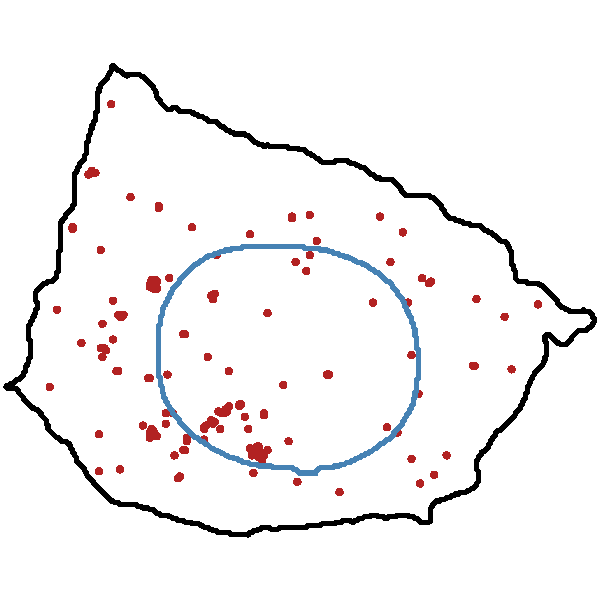
\includegraphics[width=\linewidth]{figures/introduction/real_coord_foci}
		\subcaption{Foci}
	\endminipage\hfill
	\minipage{0.2\textwidth}
		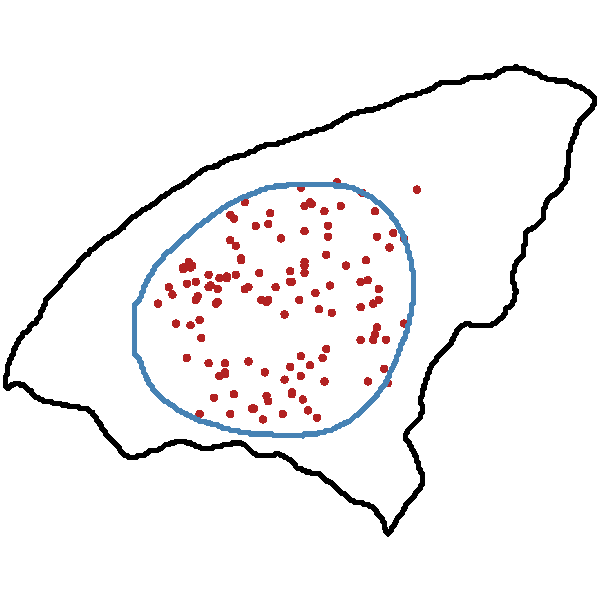
\includegraphics[width=\linewidth]{figures/introduction/real_coord_intranuclear}
		\subcaption{Intranuclear}
	\endminipage\hfill
	\minipage{0.2\textwidth}
		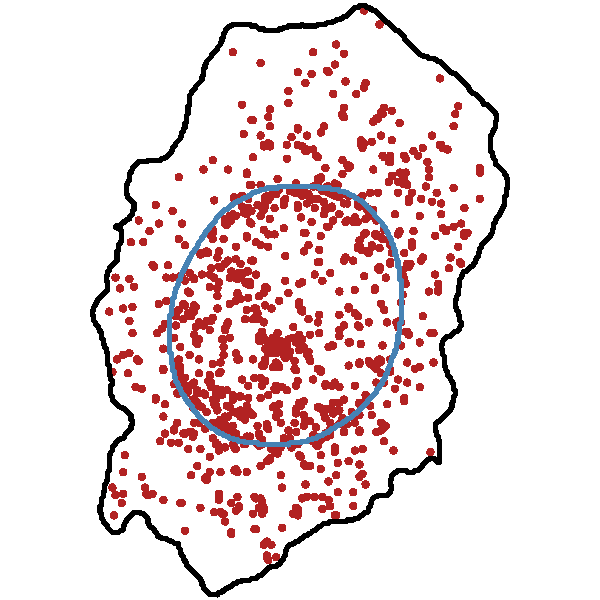
\includegraphics[width=\linewidth]{figures/introduction/real_coord_nuclear_edge}
		\subcaption{Nuclear edge}
	\endminipage\hfill
	\minipage{0.2\textwidth}
		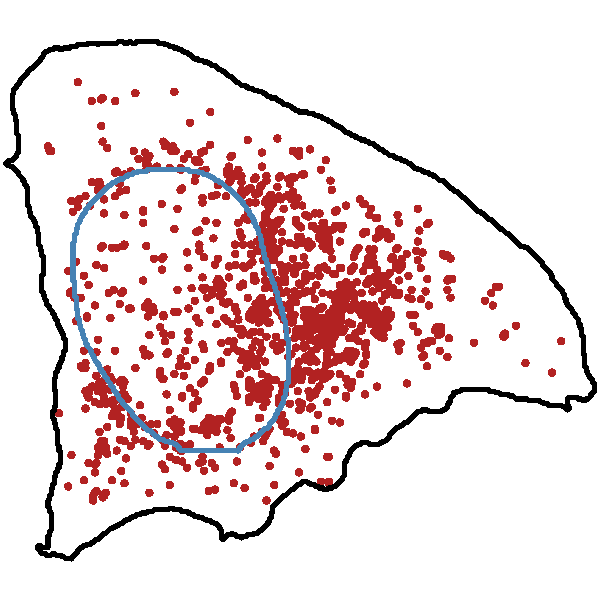
\includegraphics[width=\linewidth]{figures/introduction/real_coord_perinuclear}
		\subcaption{Perinuclear}
	\endminipage\hfill
	\minipage{0.2\textwidth}
		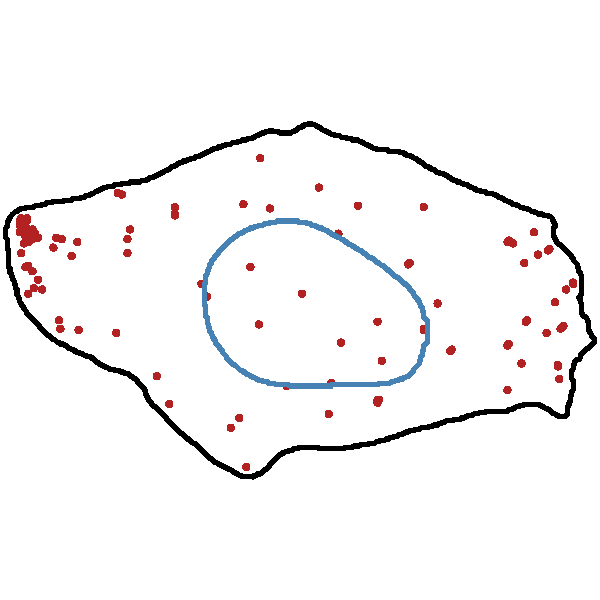
\includegraphics[width=\linewidth]{figures/introduction/real_coord_protrusion}
		\subcaption{Protrusion}
	\endminipage
	\caption{RNA localization patterns from~\cite{CHOUAIB_2020}.
	Coordinate representations with RNA spots (\textit{red}), cell membrane (\textit{black}) and nuclear membrane (\textit{blue}).
	Detection and segmentation results are extracted and visualized with \emph{bigfish}}
	\label{fig:localization_patterns_racha_features}
\end{figure}

\subsection{PointFISH}
\label{subsec:pointfish}

\subsubsection{Input preparation}

Besides the original \ac{RNA} point cloud, we can use an optional second input vector with our model.
Let's $X \in \mathbb{R}^{N \times 3}$ be the original input point cloud with $N$ the number of \ac{RNA}s.
We define our second input vector as $\tilde{X} \in \mathbb{R}^{N \times d}$ with $d \in \{1, 2, 3, 4, 5\}$.
The latter is composed of three contextual inputs.
First we can integrate morphological information by merging \ac{RNA} point cloud with 2D coordinates from the cell and the nucleus membranes.
Such coordinates are localized to the average height of the \ac{RNA} point cloud (0 if it is centered).
This morphological input substantially increases the size of the original point cloud, because we subsample 300 nodes from the cell membrane and 100 nodes from the nucleus one.
We also define an extra boolean vector to indicate the cell nodes and a second one to label the nucleus nodes.
By construction, each \ac{RNA} in the point cloud has then two \emph{False} values.
We end up with $X \in \mathbb{R}^{\tilde{N} \times 3}$ (with $\tilde{N} = N + 300 + 100$) and $\tilde{X} \in \{0, 1\}^{\tilde{N} \times 2}$ as inputs.
Second, we can compute the distance from cell and nucleus for every \ac{RNA} node.
This adds an extra input $\tilde{X} \in \mathbb{R}^{N \times 2}$.
Third, we can leverage the cluster detection algorithm from \emph{bigfish} in order to label each \ac{RNA} node as clustered or not.
It gives us a boolean $\tilde{X} \in \{0, 1\}^{N \times 1}$ to indicate if a RNA belongs to a RNA cluster of not.
Depending on whether or not we choose to add the morphological, the clustering or the distance information, we can exploit up to 5 additional dimensions of input.

\subsubsection{Model architecture}

We adopt the generic architecture introduced by PointNet~\cite{Qi_2017_CVPR}: successive point-wise representations with increasing depth followed by a max pooling operation to keep the network invariant by input permutation.
We incorporate state-of-the-art modules to learn efficient local structures within the point cloud.
As illustrated in Figure~\ref{fig:PointFISH_architecture}, we also adapt the network to the specificity of RNA point clouds.

\begin{figure}[h]
    \centering
    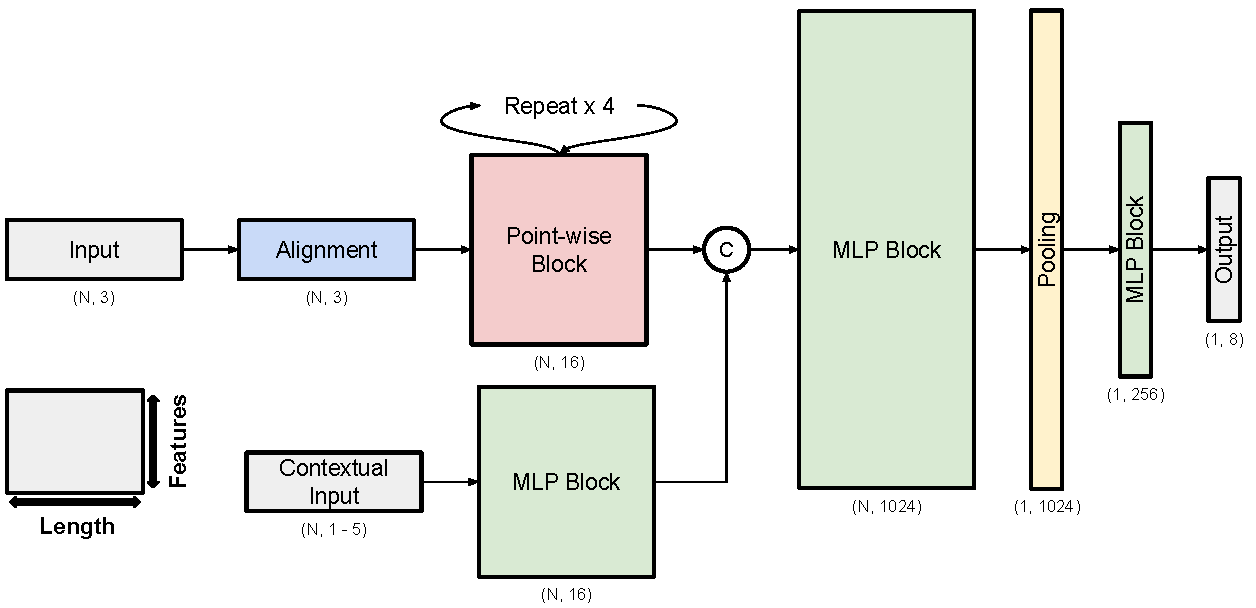
\includegraphics[width=1\textwidth]{figures/chapter4/PointFISH_architecture}
    \caption{PointFISH architecture.
	Width and height of \textit{boxes} represent output length and dimension, respectively.
	\textit{Tuples} represent output shapes}
    \label{fig:PointFISH_architecture}
\end{figure}

\paragraph{Point-wise Block}

Instead of shared MLPs like PointNet, we implement a multi-head attention layer based on point transformer layer~\cite{Zhao_2021_ICCV}.
First, we assign to each datapoint $x_i$ its 20 nearest neighbors $X(i) \subset X$, based on the euclidean distance in the features space.
We also compute a position encoding $\delta_{ij} = \theta(x_i - x_j)$ for every pair within these neighborhoods, with $\theta$ a MLP.
Three sets of point-wise features are computed for each datapoint, with shared linear projections $\phi$, $\psi$ and $\alpha$.
Relative weights between datapoints $\gamma(\phi(x_i) - \psi(x_j))$ are computed with the subtraction relation (instead of dot product as in the seminal attention paper~\cite{NIPS2017_3f5ee243}) and a MLP $\gamma$.
These attention weights are then normalized by softmax operation $\rho$.
Eventually, datapoint's feature $y_i$ is computed as weighted sum of neighbors value $\alpha(x_j)$, weighted by attention.
With the position encoding added to both the attention weights and the feature value, the entire layer can be summarized such that:

\begin{equation}
	{\displaystyle y_i = \sum_{x_j \in X(i)} \rho(\gamma(\phi(x_i) - \psi(x_j) + \delta_{ij})) \odot (\alpha(x_j) + \delta_{ij})}
\end{equation}

For a multi-head attention layer, process is repeated in parallel with independent layers, before a last linear projection merge multi-head outputs.
A shortcut connexion and a layer normalization~\cite{ba2016layer} define the final output of our multi-head attention layer.

\paragraph{Alignment Module}

Albeit optional, this module is critical.
Some papers stress the necessity to preprocess the input point cloud by learning a projection to \emph{align} the inputs coordinates in the right space~\cite{Qi_2017_CVPR,Wang_2019}.
In addition, density heterogeneity across the point cloud and irregular local geometric structures might require local normalization.
To this end, we reuse the geometric affine module described in PointMLP~\cite{ma2022rethinking} which transforms local datapoints to a normal distribution.
With $\{x_{i, j}\}_{j=1,\dots,20} \in \mathbb{R}^{20 \times 3}$, the neighborhood's features of $x_i$, we compute:

\begin{equation}
	{\displaystyle \{x_{i, j}\} = \alpha \odot \frac{\{x_{i, j}\} - x_i}{\sigma + \epsilon} + \beta}
\end{equation}

\noindent
Where $\alpha \in \mathbb{R}^3$ and $\beta \in \mathbb{R}^3$ are learnable parameters, $\sigma$ is the feature deviation across all local neighborhoods and $\epsilon$ is a small number for numerical stability.

\paragraph{Contextual Inputs}

Our \ac{RNA} point cloud does not include all the necessary information for a localization pattern classification.
Especially, we missed morphological information.
To this end, deep learning architectures allows flexible insertions.
Several contextual inputs $\tilde{X}$ can feed the network through a parallel branch, before concatenating \ac{RNA} and contextual point-wise features.
Our best model exploits cluster and distance information in addition to \ac{RNA} coordinates.

\subsection{Experiment}
\label{subsec:experiment}

\subsubsection{Training and evaluation on simulated patterns}

We train PointFISH on the simulated dataset.
Our implementation is based on TensorFlow~\cite{tensorflow_2015}.
We use Adam optimizer~\cite{Diederik_2015} with a learning rate from 0.001 to 0.00001 and an exponential decay (decay rate of 0.5 every 20,000 steps).
Model is trained for a maximum of 150 epochs, with a batch size of 32, but early stopping criterion is implemented if validation loss does not decrease after 10 consecutive epochs.
Usually model converges after 50 epochs.
We apply a 10\% dropout for the last layer and classifications are evaluated with a categorical cross entropy loss.
Even if localization patterns are not necessarily exclusive, for the simulations we trained the model to predict only one pattern per cell.
For this reason, we did not simulate mixed patterns and assume it could help the model to learn disentangled representations.
Training takes 6 to 8 hours to converge with a Tesla P100 GPU.

A first evaluation can be performed on the simulated test dataset.
Because each pattern is equally generated, a simple accuracy metric is enough.
On experimental dataset, imbalanced between localization patterns implies a more robust metric like F1-score.
With our best PointFISH models, we obtain a general F1-score of 95\% over the different patterns (see confusion matrix~\ref{fig:confusion_matrix}).

\begin{figure}[h]
    \centering
    \includegraphics[width=0.7\textwidth]{figures/chapter4/confusion_matrix}
    \caption{Confusion matrix with simulated patterns (normalized over the \textit{rows})}
    \label{fig:confusion_matrix}
\end{figure}

\subsubsection{Embedding extraction}

From a trained PointFISH model we can remove the output layer to get a feature extractor that computes a 256-long embedding from a \ac{RNA} point cloud.

\paragraph{Learned embedding}

We compute the embedding for the entire cell population studied in~\cite{CHOUAIB_2020}.
All the 9170 cells can be visualized in 2D using a UMAP projection~\cite{McInnes2018}.
In Figure~\ref{fig:umap_real} every point represents a cell.
Among the 810 annotated cells, those with a unique pattern are colored according to the localization pattern observed in their \ac{RNA} point cloud.
The rest of the dataset remains gray.
Overall, PointFISH embedding discriminates well the different localization patterns.
Intranuclear, nuclear edge and perinuclear cells form distinct clusters, despite their spatial overlap, as well as protrusions.
Cells with foci can be found in a separated clusters as well, but also mix with nuclear and perinuclear patterns.
This confusion is not surprising as a large number of cells in the dataset present a nuclear-related foci pattern: cells have \ac{RNA}s clustered in foci, which in turn are close to the nuclear envelope, in which case the cell would be labeled with both patterns.

\begin{figure}[h]
    \centering
    \includegraphics[width=\textwidth]{figures/chapter4/umap_real}
    \caption{UMAP embedding with learned features.
	Each point is a cell from dataset~\cite{CHOUAIB_2020}.
	Manually annotated cells are colored according to their localization pattern}
    \label{fig:umap_real}
\end{figure}

\paragraph{Supervised classification}

Because PointFISH already return meaningful embeddings, we can apply a simple classifier on top of these features to learn localization patterns.
We use the 810 manually annotated cells from the experimental dataset.
We compare the 15 hand-crafted features selected in~\cite{CHOUAIB_2020} with our learned embedding.
Every set of features is rescaled before feeding a classifier.
Expert features includes:

\begin{itemize}
	\item The number of foci and the proportion of clustered \ac{RNA}.
	\item The average foci distance from nucleus and cell (normalized by the expected distance with a random foci distribution).
	\item The proportion or \ac{RNA} inside nucleus.
	\item The average \ac{RNA} distance from nucleus and cell (normalized by the expected distance with a random \ac{RNA} distribution).
	\item The number of \ac{RNA}s detected in cell extensions (normalized by the expected number with a random \ac{RNA} distribution) and the peripheral dispersion index~\cite{stueland_rdi_2019}.
	\item The number of \ac{RNA}s within different relevant subcellular regions (normalized by the expected number with a random \ac{RNA} distribution).
\end{itemize}

\begin{figure}[h]
    \centering
	\includegraphics[clip, trim=0cm 0cm 0cm 1cm, width=\textwidth]{figures/chapter4/f1_SVC}
    \caption{F1-score distribution with localization pattern classification (SVC model)}
    \label{fig:f1_SVC_real}
\end{figure}

We design 5 binary classification tasks, one per localized pattern (random pattern is omitted).
The classifier is a SVC model~\cite{chang2011libsvm}.
For evaluation purpose, we apply a nested cross-validation scheme.
First a test dataset is sampled the dataset (20\%), then the remaining cells are used with a gridsearch to fit an optimal SVC model (with a 20\% validation split).
Parameters grid includes the choice between a linear or a RBF kernel and the strength of the regularization.
The entire process is repeated 50 times, with different test split, and F1-score for each classification task is returned.
This full evaluation pipeline is implemented with \emph{scikit-learn}~\cite{scikit-learn}.
F1-score's distribution over 50 splits are summarized in Figure~\ref{fig:f1_SVC_real}.
Learned features match performances of hand-crafted features selected for the tasks.
While the recognition of localization in protrusions is slightly worse, it is important to point out that we did not include simulations of this patterns in the training dataset.

\subsubsection{Ablation study}

We perform several ablation studies to evaluate the impact of different components in PointFISH model.
In the point cloud literature, papers often propose new modules to improve network's performances, but they implement them in slightly different architectures.
Heterogeneity in terms of normalization, latent dimensions or layer size complicate comparisons between techniques.
In order to isolate the importance of each element, we use a template architecture as illustrated in Figure~\ref{fig:PointFISH_architecture}.
Instead of comparing PointFISH with DGCNN, we compare PointFISH with an equivalent networks where attention layers are replaced by EdgeConv~\cite{Wang_2019}.
The rest of the network remains strictly identical.

\paragraph{Additional input}

\begin{wraptable}{R}{0.60\textwidth}
	\centering
	\begin{tabular}{| c | c | c | c |}
		\hline
		Distance & Cluster & Morphology & F1-score \\
		\hline
		\ding{55} & \ding{55} & \ding{55} & 0.42\\
		\checkmark & \ding{55} & \ding{55} & 0.74\\
		\ding{55} & \checkmark & \ding{55} & 0.45\\
		\checkmark & \checkmark & \ding{55} & $0.81^{\ast}$\\
		\checkmark & \checkmark & \checkmark & \textbf{0.82}\\
		\hline
	\end{tabular}
	\caption{Impact of contextual inputs.
	F1-score is averaged over 4 trainings with different random seeds.
	Best model is in bold.
	Reference model is labelled with $\ast$}
	\label{table:extra_inputs}
\end{wraptable}

We compare the use of \ac{RNA} point cloud only as input or the inclusion of contextual inputs through a parallel branch.
\ac{RNA} coordinates do not have any morphological information about the cell.
In Table~\ref{table:extra_inputs}, this design logically returns the lowest F1-score.
Three additional inputs are available: \ac{RNA} distance from cell and nucleus (\emph{distance}), \ac{RNA} clustering flag (\emph{cluster}) and the integration of cell and nucleus membrane coordinates (\emph{morphology}).
Best performances are reached with at least distance and cluster information.
Cell and nucleus coordinates do not increase significantly the classification and dramatically increase the computation time of the model (we need to process a larger point cloud).
In particular, cluster information greatly improves foci pattern recognition while distances boost others localization patterns.

\paragraph{Alignment module and Point-wise block}

To measure the impact of the geometric affine module~\cite{ma2022rethinking} we compare it with the TNet module implemented in PointNet~\cite{Qi_2017_CVPR}.
We also design a variant TNetEdge where MLP layers extracting point-wise independent features are replaced with EdgeConv layers.
Results are reported in Table~\ref{table:ablation}.
An alignment block seems critical at the beginning of the network.
However, the geometric affine module is both more efficient (F1-score of 0.81) and much lighter than TNet and TNetEdge.

From PointNet and DGCNN seminal papers we also compare the use of their respective point-wise blocks compare to our multi-head attention layer.
As expected, EdgeConv blocks convey a better information than PointNet by exploiting local neighborhood within point cloud (F1-score of 0.78 and 0.75 respectively).
Yet, they do not match the performance of multi-head attention layer.

Concerning these layers, we evaluate how the number of parallel heads can influence the performance of PointFISH.
By default, we use 3 parallel attention layers to let the model specialized its attentions vectors, but we also test 1, 6 and 9 parallel heads.
In Table~\ref{table:ablation} we only observe a slight benefit between the original point transformer layer~\cite{Zhao_2021_ICCV} (without one attention layer) and its augmented implementation.

% multiscale
% k neigbors

\paragraph{Latent dimensions}

The second part of PointFISH architecture is standardized: a first MLP block, a max pooling operation, a second MLP block and the output layer.
We quantify the impact of additional MLP layers within these blocks.
Our reference model returns an embedding with 256 dimensions (before the output layer).
In a MLP block, we use ReLU activation and layer normalization, but also increase or decrease the depth by a factor 2 between layers.
Before the pooling layer, the first MLP block includes 4 layers with an increasing depth (128, 256, 512 and 1024).
After the pooling layer, the second MLP block includes 2 layers with a decreasing depth (512 and 256).
Similarly, to return 128, 64 or 32 long embeddings, we implement 6 (128, 256, 512, pooling, 256 and 128), 5 (128, 256, pooling, 128 and 64) or 4 final layers (128, pooling, 64 and 32).
We observe in Table~\ref{table:ablation} a fall in performance for the lowest dimensional embedding (64 and 32).
This hyperparameter is also critical to design lighter models, with a division by 4 in terms of trainable parameters between a 256 and a 128 long embedding.

\begin{table}[h]
	\centering
	\begin{tabular}{| c | c | c | c | c | c |}
		\hline
		Alignment & Point-wise block & \# heads & \# dimensions & \# parameters & F1-score \\
		\hline\hline
		- & Attention layer & 3 & 256 & 1,372,608 & 0.73\\
		TNet & Attention layer & 3 & 256 & 1,712,521 & 0.74\\
		TNetEdge & Attention layer & 3 & 256 & 1,589,321 & 0.74\\
		\hline\hline
		Affine & MLP & - & 256 & 1,374,526 & 0.75\\
		Affine & EdgeConv & - & 256 & 1,387,006 & 0.78\\
		\hline\hline
		Affine & Attention layer & 9 & 256 & 1,403,334 & \textbf{0.82}\\
		Affine & Attention layer & 6 & 256 & 1,387,974 & \textbf{0.82}\\
		Affine & Attention layer & 3 & 256 & 1,372,614 & $0.81^{\ast}$\\
		Affine & Attention layer & 1 & 256 & 1,362,374 & 0.81\\
		\hline\hline
		Affine & Attention layer & 3 & 128 & 352,966 & 0.81\\
		Affine & Attention layer & 3 & 64 & 97,094 & 0.77\\
		Affine & Attention layer & 3 & 32 & 32,646 & 0.75\\
		\hline
	\end{tabular}
	\caption{Ablation studies on experimental dataset~\cite{CHOUAIB_2020}.
	F1-score is averaged over 4 trainings with different random seeds.
	Best models are bold.
	Reference model is labelled with $\ast$}
	\label{table:ablation}
\end{table}

\subsection{Discussion}
\label{subsec:discussion}

Being able to directly process list of points provides the community with a tool to integrate large datasets obtained with very different techniques on different model systems.
While the actual image data might look strikingly different between such projects, they can all be summarized by segmentation masks of nuclei and cytoplasm, and a list of coordinates of \ac{RNA} locations.
Besides being a straightforward approach, having methods that act directly on point clouds is also a strategic advantage.

The idea of training on simulated data provides us the opportunity to query datasets with respect to new localization patterns that have not yet been observed, and for which we do not have real examples so far.
In addition, this strategy allows us to control for potential confounders, such as cell morphology, or number of \ac{RNA}s.

We finally provide a generic method that can leverage these simulations, without the tedious process of handcrafting new features.
It is not necessary that the simulated patterns are optimized as to resemble real data.
They rather serve as a pretext task.
If a network is capable of distinguishing the simulated patterns, chances are high that the corresponding representation is also informative for slightly or entirely different patterns.
Likewise, representations trained on ImageNet can be used for tumor detection in pathology images.
We show this by omitting the protrusion pattern from the simulation.
Indeed, in Figure~\ref{fig:umap_real}, the protrusion patterns live in a particular region of the feature space, without specific training.

% reference ImageNet
% reference tumor detection in pathology images

As a future work, a first valuable task would be the development or the sourcing of annotated datasets with various cell lines and imaging conditions.
The difficulty to gather experimental training datasets can be overcome by simulations.
However, we still need to extend our evaluation across different benchmarks to assess the robustness of a point cloud model.
Among the examples of interest, recent publications~\cite{savulescu_interrogating_2021,mah_bento_2022} evaluate their methods on their own datasets, which include \ac{RNA} localization annotations.
Second, a better engineering of PointFISH could make contextual inputs irrelevant and only base predictions on the point cloud coordinates.
A third potential improvement concerns the segmentation.
We exploit so far a 2D segmentation because it is the more frequent usecase and the task for which we have a large number of trained models available.
Yet, a 3D segmentation mask would allow a more complete 3D point cloud mixing \ac{RNA} and cell datapoints.
This could also dramatically improve pattern representation.
Last but not least, training a point cloud model with a self-supervised training procedure would result in task-independent representations.
This could eventually help to generalize over unknown localization patterns.

\section{Conclusion}
\label{sec:analysis_conclusion}

We first present the coordinate representation of the cell, from which we base our feature engineering and our statistical analysis.
On the top of existing solutions to extract \ac{RNA} spots and cell morphology coordinates, we then list the different hand-crafted features we designed to quantify and classify \ac{RNA} localization patterns.
These features are implemented in \emph{bigfish.classification}.
Lastly, in the third section, we propose to directly process the extracted point clouds, without the need to design handcrafted features.
For this, we leverage coordinates of simulated localization patterns to train a specifically designed neural network taking as input a list of points and associated features that greatly enhance generalization capabilities.
Recent advances in point cloud analysis through deep learning models allows us to build a flexible and scalable pipeline that fit with \ac{RNA} point cloud specificity.
We show that this method is on par with carefully designed, handcrafted feature sets.

% learned features from convnet
% from features engineering to simulation engineering
% limitations % 7400 22
%\part{Applications}
%!TEX root = ../main.tex

\graphicspath{{./figures/chapter5/}}

\chapter{RNA localization by the numbers}
\label{ch:chapter5}

\minitoc
\newpage

In this chapter, I present several applications of the pipeline described in the previous chapters.
More specifically, I analyze experimental datasets in order to explore, quantify and validate biological insights about \ac{mRNA} localization.
Results from this chapter are computed from three different high content screening studies, totaling tens of transcripts observed through thousands of bioimages.

In the first section, I develop a general classification pipeline to identify generic \ac{mRNA} localization patterns from \ac{smFISH} images~\cite{CHOUAIB_2020}.
In the second section, exploiting the same dataset, I focus on a specific and novel clustering pattern: the translation factories.
These first two sections describe the work published in:

\begin{center}
	\color{green}
	R. Chouaib, A. Safieddine, et al. (2020), \textit{A dual protein-mRNA localization screen reveals compartmentalized translation and widespread co-translational RNA targeting}, Developmental Cell 54 (6), 773.
\end{center}

In the third section, I exploit a \ac{GFP} channel to visualize and detect centrosomes.
I observed a centrosomal localization patterns for different transcripts and mitosis phases~\cite{safieddine_choreography_2021}.
This work was published in:

\begin{center}
	\color{green}
	A. Safieddine, E. Coleno, et al. (2021), \textit{A choreography of centrosomal mRNAs reveals a conserved localization mechanism involving active polysome transport}, Nature Communications 12 (1), 1352.
\end{center}

In the fourth section, I detail several transcripts with a protrusion localization pattern~\cite{pichon_kinesin_2021}.
This last section mainly describes results presented in:

\begin{center}
	\color{green}
	X. Pichon, K. Moissoglu, et al. (2021), \textit{The kinesin KIF1C transports APC-dependent mRNAs to cell protrusions}, RNA 27 (12), 1528.
\end{center}

\section{A systemic quantification of RNA localization}
\label{sec:general_pattern_recognition}

In~\cite{CHOUAIB_2020}, I have implemented a quantitative pipeline to analyze the localizations of \ac{mRNA} molecules.
This work lays the foundation of the future Python packages developed in FISH-quant V2~\cite{Imbert_fq_2022}.
My contribution consists in classifying individual cells with one or several \ac{RNA} localization patterns.

\subsection{Introduction}
\label{subsec:introduction_general_pattern}

Most of \ac{mRNA}s have a random distribution throughout the cytoplasm, but some of them localize in specific subcellular regions.
This phenomenon has been previously reviewed in different papers~\cite{Blower_2013, Jung_2014, Eliscovich_2017, Bovaird_2018}.

Such localization can be related to either the \ac{RNA} metabolism, for example with untranslated \ac{mRNA}s stored and repressed in \ac{P-bodies} (but not degraded~\cite{Hubstenberger_2017}), or the protein metabolism with locally translated proteins.
This local synthesis concerns both mature proteins and nascent peptides.
Different cellular processes imply the delivery of mature proteins in specific subcellular regions and a local regulation of the proteome.
Local translation can contributes to cell fate determination during metazoan development, as observed in~\cite{melton_translocation_1987} with a clear modification of the Vg1 \ac{RNA} spatial distribution between mature and immature Xenopus oocytes.
In these same Xenopus embryos, cyclin B1 \ac{mRNA}s localized at the mitotic apparatus could also play an important role in the rapid cell division cycles observed during early embryogenesis~\cite{Groisman_2000}.
In mammal cells, \ac{RNA} localization influences cell polarization and motility, usually through actin localization at the cell edge~\cite{Lawrence_1986}.
Locally translated proteins are also known to be involved in axonal growth and so neural plasticity~\cite{VanDriesche_2018}.
Finally, by precisely controlling the \ac{mRNA} localization and the subsequent translation process, cells can avoid to release proteins at inappropriate places~\cite{Muller_myelin_2013} and help the synthesis of protein complexes~\cite{pichon_visualization_2016}.

Several mechanisms will drive the localization of \ac{mRNA}s.
Sometimes the nascent peptide can serve as a targeting signal, but most of the time the \ac{RNA} molecule itself will initiate its localization.
\ac{RNA} can also be trapped in specific subcellular compartments.
The molecule often include a zip-code sequence that is read by a \ac{RBP} and starts the assembly of a transport complex comprising different organelles or motor proteins.
Such complex can then directly convey the \ac{RNA} along the cytoskeleton~\cite{Blower_2013}.
Coupled with an anchoring mechanism at the targeted destination, it provides a better stability of the \ac{RNA} localization.

In~\cite{CHOUAIB_2020}, we claim that a global view of local translation in the whole cell and at the genomic level is still to come, despite recent progress.
In a pioneering work on Drosophila embryogenesis~\cite{lecuyer_global_2007}, authors analyze 3,370 genes and find that 71\% of them encode a transcript with a non-uniform localization pattern.
In human cell lines recent studies exploit and improve \ac{smFISH} techniques to image thousands of \ac{mRNA}s in the perinuclear region, the mitochondria and the cell membrane~\cite{battich_image-based_2013, Chen_2015, eng_seqfish_2019, Xia_2019}.
We take a step forward in studying \ac{mRNA} localization with human cell lines and a systematic approach.
We perform a quantitative analysis leveraging supervised and unsupervised methods in order to recognize up to 6 different localization patterns.
The current section emphasizes this quantitative pipeline that contributes to make our analysis scalable and more robust.

\subsection{Materials and methods}
\label{subsec:materials_general_pattern}

The quantitative pipeline used in this study and the existing work in FISH-quant V1 are the building blocks of FISH-quant V2.
Therefore, the various methods presented here were not yet packaged in \emph{bigfish}, but Python libraries that formed its foundation were already in used.
This work is developed in Python and the code repository is public\footnote{\url{https://github.com/Henley13/paper_translation_factories_2020}}.

\subsubsection{Experimental data}

At first more than 500 genes have been manually analyzed to identify potential transcripts with non random localization patterns within the cell.
In addition to different qualitative and manual observations performed over this dual \ac{RNA}-protein localization screen, we also develop a quantitative pipeline to systematically classify transcripts' localization patterns.
To this end, I exploit a dataset of 526 \ac{FoV}s, combining DAPI and \ac{smFISH} channels as illustrated in Figure~\ref{fig:fov_racha}.
The raw images stacks several 2D acquisitions to gather a 3D information of the \ac{FoV} with a z-spacing of 0.3μm.
Acquisitions are performed with a Zeiss Axioimager Z1 widefield microscope or a Nikon Ti fluorescence microscope, on human cell lines HeLa.
In total, this dataset is built from 57 independent experiments gathering observations from 27 different \ac{mRNA}s under different experimental conditions.

\begin{figure}[]
    \centering
    \includegraphics[width=\textwidth]{figures/chapter5/FoV_DYNLL2}
    \caption[Contrasted image with Dapi and smFISH channels]{Contrasted image with Dapi (\textit{left}) and smFISH (\textit{right}) channels.
	Images are projected in 2D.
	Targeted transcript is DYNLL2.
	Plot built with \emph{bigfish}}
    \label{fig:fov_racha}
\end{figure}

\subsubsection{Semi-automated RNA detection}

\ac{RNA} detection is performed with a Python implementation of FISH-quant v1~\cite{mueller_fish-quant_2013}.
I apply a \ac{LoG} filter on the 3D \ac{smFISH} images, then a local maximum detection algorithm.
However, a threshold value has to be set manually for every experiment to discriminate the actual spots from the noisy background blobs.
Large agglomeration of spots are decomposed with a gaussian mixture model, following~\cite{samacoits_computational_2018}.
Ultimately, \ac{RNA} clusters - namely foci - are detected with a DBSCAN algorithm~\cite{ester_density-based_1996} applied on the detected spots.
According to the way a DBSCAN cluster samples, a foci is then defined as a set of at least 5 points where for each point there is at least one other point from the foci within a 350 nanometers distance.
All foci overlapping the nuclear area in the projected 2D images are considered as a transcription site and removed from the analysis.
Percentages of \ac{RNA} in foci are then calculated as number of \ac{RNA} inside the cytoplasmic foci divided by the number of cytoplasmic \ac{RNA}s.

There are two main differences compared to the current detection methods implemented in FISH-quant and presented in Chapter~\ref{ch:chapter2}: a detection threshold has to be set manually and the decomposition of agglomerated spots has since been simplified.

\subsubsection{Cell and nucleus segmentation}

Nucleus segmentation is performed from the DAPI channel and cell segmentation from the cell autofluorescence in the \ac{smFISH} channel.
Segmentation is performed in 2D for both nuclei and cells, thus 3D images are projected in two dimensions using their maximal local focus values~\cite{tsanov_smifish_2016}.

Nuclei are segmented with NucleAIzer~\cite{hollandi_nucleaizer_2020}, a deep neural network pipeline trained with the annotations from the Data Science Bowl 2018 challenge\footnote{\url{https://www.kaggle.com/c/data-science-bowl-2018}}.
This pipeline is based on a Mask R-CNN architecture~\cite{He_2017_ICCV}, with optionally a fine-tuning of the segmented boundaries with a U-Net model~\cite{Ronneberger_unet}.
After a first round of segmentation, some nuclei are missing, so I remove the segmented nuclei from the DAPI channel and feed NucleAIzer with the remaining nuclei for a second round of segmentation.
Removing the segmented nuclei from the original image implies some morphological mathematics techniques as described in Chapter~\ref{ch:chapter3}.
This technique is now implemented in FISH-quant.

Cells are segmented with a watershed algorithm using nucleus masks as seeds.
A threshold value is set manually for every experiment to discriminate the cell surface from the background.
In case of poor results, some segmentation masks are corrected manually.
This is especially the case for transcript that tend to localize in cell protrusion.
Indeed, such localization pattern is highly sensitive to the segmentation accuracy.

\subsubsection{Localization feature engineering}

Based on the segmentation masks and the coordinates of the detected spots, I identify 9,710 individual cells with an average of 346 \ac{RNA}s per cell.
For each cell, I collect the cell and nucleus masks in 2D, the \ac{RNA} and the potential cluster coordinates in 3D.
In addition I save an image of the cell, for visualization purpose, and different information about the experiment (the presence of a treatment, the targeted gene, etc.).
Cropped cells, empty cells or cells with less than 30 detected \ac{RNA} inside are removed.
At this point, I have a coordinate representation of every cell, as presented in Chapter~\ref{ch:chapter4}.

I design and compute a set of 15 features to describe the spatial distribution of points inside the cell:
\begin{itemize}
	\setlength\itemsep{0.1em}
	\item The number of foci.
	\item The proportion of \ac{RNA} inside foci.
	\item The proportion of \ac{RNA} inside the nucleus.
	\item The average \ac{RNA} distance to the cell membrane, normalized by the value obtained under a uniform \ac{RNA} distribution.
	\item The average \ac{RNA} distance to the nucleus membrane, normalized by the value obtained under a uniform \ac{RNA} distribution.
	\item The average foci distance to the cell membrane, normalized by the value obtained under a uniform foci distribution.
	\item The average foci distance to the nucleus membrane, normalized by the value obtained under a uniform foci distribution.
	\item The proportion of \ac{RNA} inside cell protrusion.
	A protrusion region is defined by calculating the difference between the segmented cellular region and its morphological opening with a large window.
	\item The peripheral dispersion index, defined as the squared point distance to the centroid of the cell and normalized by the value obtained under a uniform \ac{RNA} distribution.
	\item The number of \ac{RNA}s within 515 nm from the nucleus membrane, normalized by the value obtained under a uniform \ac{RNA} distribution.
	\item The number of \ac{RNA}s between 515 nm and 1030 nm from the nucleus membrane, normalized by the value obtained under a uniform \ac{RNA} distribution.
	\item The number of \ac{RNA}s between 1030 nm and 1545 nm from the nucleus membrane, normalized by the value obtained under a uniform \ac{RNA} distribution.
	\item The number of \ac{RNA}s between 0 nm and 515 nm from the cell membrane, normalized by the value obtained under a uniform \ac{RNA} distribution.
	\item The number of \ac{RNA}s between 515 nm and 1030 nm from the cell membrane, normalized by the value obtained under a uniform \ac{RNA} distribution.
	\item The number of \ac{RNA}s between 1030 nm and 1545 nm from the cell membrane, normalized by the value obtained under a uniform \ac{RNA} distribution.
\end{itemize}

The apparent precision of the nanometer distances is just an artifact as the concentric regions are delimited visually from a sample of cell images.
Therefore, the width of these regions are defined in pixels, more precisely, with a 5 pixels width and a pixel size of 103 nm.

\subsubsection{Binary classification models}

\begin{figure}[]
	\centering
	\minipage{0.2\textwidth}
		\includegraphics[trim={0.5cm 0.5cm 0.5cm 0.5cm},clip,width=\linewidth]{figures/chapter5/plot_foci}
		\subcaption{Foci}
	\endminipage\hfill
	\minipage{0.2\textwidth}
		\includegraphics[trim={0.5cm 0.5cm 0.5cm 0.5cm},clip,width=\linewidth]{figures/chapter5/plot_intranuclear}
		\subcaption{Intranuclear}
	\endminipage\hfill
	\minipage{0.2\textwidth}
		\includegraphics[trim={0.5cm 0.5cm 0.5cm 0.5cm},clip,width=\linewidth]{figures/chapter5/plot_nuclear}
		\subcaption{Nuclear edge}
	\endminipage\hfill
	\minipage{0.2\textwidth}
		\includegraphics[trim={0.5cm 0.5cm 0.5cm 0.5cm},clip,width=\linewidth]{figures/chapter5/plot_perinuclear}
		\subcaption{Perinuclear}
	\endminipage\hfill
	\minipage{0.2\textwidth}
		\includegraphics[trim={0.5cm 0.5cm 0.5cm 0.5cm},clip,width=\linewidth]{figures/chapter5/plot_protrusion}
		\subcaption{Protrusion}
	\endminipage
	\caption[RNA localization patterns]{RNA localization patterns from~\cite{CHOUAIB_2020}.
	Coordinate representations with RNA spots (\textit{red}), cell membrane (\textit{black}) and nuclear membrane (\textit{blue}).
	Detection and segmentation results are extracted and visualized with \emph{bigfish}}
	\label{fig:localization_patterns_racha_features}
\end{figure}

I use these hand-crafted features to train several binary classifiers, one for each localization pattern we want to recognize.
Five specific localization patterns are defined - foci, intranuclear, nuclear edge, perinuclear, protrusion - and the random pattern is considered as a default one.
Figure~\ref{fig:localization_patterns_racha_features} illustrates an example of these patterns with a coordinate representation.

To train the classifiers, manual annotations are needed as a ground truth.
I generate panels with the cropped original image of the individual cells and their coordinate representations.
These panels are then manually tagged with the appropriate localization pattern.
The manual classification result has been independently checked by several trained microscopists.
Ultimately, I end up with 810 annotated cells.
Counts of the annotations are presented in Table~\ref{table:real_dataset_chapter5}.

\begin{wraptable}{L}{0.50\textwidth}
	\centering
	\begin{tabular}{| c | c |}
		\hline
		Pattern & \# of cells \\
		\hline
		Random & 372\\
		Foci & 198\\
		Intranuclear & 73\\
		Nuclear edge & 87\\
		Perinuclear & 64\\
		Protrusion & 83\\
		\hline
	\end{tabular}
	\caption[Count of annotated cells]{Annotated cells}
	\label{table:real_dataset_chapter5}
\end{wraptable}

One way to evaluate how relevant is the feature space is to investigate the distribution of the annotated cells within it.
To do so, I reduce the dimensionality with a \ac{t-SNE} transformation~\cite{vandermaaten_2008} in order to visualize the features point cloud.
From the multi-dimensional feature space, I obtain a 2D vector representation I can plot.
In term of setting, I initialize the \ac{t-SNE} with a PCA transformation first and use a perplexity value of 30.

I also define a supervised learning problem with the training of 5 independent binary Random Forest classifiers~\cite{breiman_random_2001}.
The choice to design the problem as several binary ones instead of one multi-class problem allows me to define the localization patterns as non mutually exclusives.
Indeed, an individual cell can display several patterns at the same time, like \ac{RNA} clusters (foci) localizing around the nuclear membrane (nuclear edge).
For each model, I build a training set including all the cells of one class and a subsampling of cells from others classes, such that the imbalance is 1:4 for the positive class.
This is a ''one vs.\ all'' training strategy.
Eventually, I exploit the \ac{OOB} error allowed by the random forest design.
In such manner, the model can ''be fit in one sequence, with cross-validation being performed along the way.''~\cite{hastie_elements_2009}.
Random forest is an ensemble model of tree classifiers.
Each tree is trained on a subsample of the observations and a subset of features.
This ensembling framework makes random forest quite robust to overfitting.
For every sample, an \ac{OOB} prediction can be computed using only the trees fitted without the sample.
I initialize the random forests with 100 trees, a maximal depth of 3 and a minimum number of samples per splitter node of 2.
During the training, for each split, I consider a subset of 10 features and entropy criterion.
In addition, input dataset is rescaled to have zero mean and unit variance.

\subsection{Results}
\label{subsec:results_general_pattern}

Thanks to their design or their normalization, the selected spatial features are mostly invariant to \ac{RNA} concentration.
They enable the use of unsupervised or supervised methods to classify cells among several localization patterns.

\subsubsection{Unsupervised visualization}

\begin{figure}[]
    \centering
    \includegraphics[width=\textwidth]{figures/chapter5/tsne_annotation_legend}
    \caption[t-SNE embedding of experimental cells]{t-SNE embedding from~\cite{CHOUAIB_2020}.
	Each point is a cell in the feature space after a t-SNE transformation.
	Manually annotated cells are colored according to their localization pattern.
	Cells that were not annotated or that had multiple patterns are colored in gray}
    \label{fig:tsne_annotation_racha}
\end{figure}

The resulting embedding from the \ac{t-SNE} algorithm can be observed in Figure~\ref{fig:tsne_annotation_racha}.
Cells with different patterns are localized in different regions of the embedded feature space.
Moreover, cells with the same annotations cluster in the same regions whether they correspond to the same gene or not.
With these observations it seems the hand-crafted features capture key information of the localization patterns and summarize well the manual annotations.

Initialized with a PCA transformation, a \ac{t-SNE} algorithm better preserves the global structure, thus enabling more relevant global interpretation.
In particular, we can discriminate at the top a large cluster of cells with a potential foci pattern from the rest of the cell population.
The resulting embedding also seems to polarize between nucleus-related patterns (bottom left) and the cell-related patterns (top right).
This polarization remains even among the subpopulation with potential foci pattern.
Such conclusion validates the design to let a cell being classified with several non-exclusive localization patterns.
Indeed, a foci can be localized in a relevant subcellular compartment.

\subsubsection{Gene aggregated classifications}

Not surprisingly, a feature space that discriminates well between classes also performs well when fed into a robust random forest classifier.
The \ac{OOB} accuracy score obtained for the different patterns is between 0.93 and 0.99, while a dummy classifier would return a 0.8 accuracy score (the dataset is built with 20\% positive samples).
The intranuclear pattern is the easiest to recognize.
In fact, it could be predicted by just thresholding the proportion of \ac{RNA} inside nucleus (almost all intranuclear cells have more than 80\% of their\ac{RNA}s that localize inside the nucleus).
On the opposite, the nuclear edge and perinuclear patterns are the most difficult to classify due to possible confusion with a random pattern or the lack of annotated cells.

\begin{wraptable}{R}{0.50\textwidth}
	\centering
	\begin{tabular}{| c | c |}
		\hline
		Pattern & Accuracy score\\
		\hline
		Random & -\\
		Foci & 0.95\\
		Intranuclear & 0.99\\
		Nuclear edge & 0.93\\
		Perinuclear & 0.93\\
		Protrusion & 0.94\\
		\hline
		\textit{Dummy classifier} & \textit{0.80}\\
		\hline
	\end{tabular}
	\caption[Random forest accuracy]{Random forest accuracy (OOB)}
	\label{table:accuracy_oob}
\end{wraptable}

For each cell, I can compute 5 binary predictions, one per pattern.
Individual cell is assigned to a pattern if the probability given by the random forest classifier for that pattern is higher than 0.5.
If no pattern is detected, cell is classified with a random localization pattern.
In total, I analyze 27 different genes through a population of 9,710 cells, with only one kind of transcript being targeted per cell.
The number of cells identified per gene varies, thus predictions are aggregated at the gene level.
This aggregation also facilitates the validation of biological insights and helps understanding the mechanism at stake for specific group of genes.
For every gene, I compute the proportion of cells displaying each indicated localization pattern.
Results are eventually reported in a heat map~\ref{fig:heatmap_racha}, for every gene and pattern.
Importantly, row values does not sum to one because classifiers (and so columns predictions) are independent.

\begin{figure}[]
    \centering
    \includegraphics[width=\textwidth]{figures/chapter5/heatmap_racha_2}
    \caption[Heat maps with localization pattern classification results]{Heat maps from~\cite{CHOUAIB_2020} with the fraction of cells classified in the indicated pattern.
	(\textit{Top heat map}) Genes whose RNAs shows a localization preference.
	Only values significantly different from negative controls are colored (p-value computed with Fisher's exact test).
	(\textit{Bottom heat map}) Negative control with genes whose RNAs localize randomly.
	(\textit{Left bars}) Manual annotations of the genes are indicated with the same color scheme than Figure~\ref{fig:tsne_annotation_racha}}
    \label{fig:heatmap_racha}
\end{figure}

We manually identify a group of random genes that can be used as a control group: KIF20B, MYO18A, SYNE2 and PLEC.
Therefore, it is possible to perform statistical testing over the aggregated predictions.
A Fisher's exact test can measure if the proportion of cells observed with a pattern is significantly greater than the proportion observed in the control group (with a $\text{p-value} < 10^{-3}$).
Genes whose transcripts present a significant localization preference are reported in Figure~\ref{fig:heatmap_racha}.

Overall, we observe consistent results with the manual annotations performed by the biologists (the colored annotations in the \ac{t-SNE} plot~\ref{fig:tsne_annotation_racha} and the vertical colored bars next to the heat map~\ref{fig:heatmap_racha}).
The agreement between automated and manual classification holds with a high degree of statistical significance, except for FLNA and KIF5B.
FLNA transcripts are manually identified with a potential cell edge pattern.
However, such localization is difficult to recognize with the quantitative pipeline, mostly because the pattern is visible in 3D while my cell segmentation, and the spatial features resulting from it, is in 2D.
For these reasons we do not study in depth this localization pattern.

\subsubsection{Recognition of five localization patterns}

Apart from KIF5B, others transcripts localizing in cytoplasmic extensions (or protrusions) are correctly identified: KIF1C, KIF4A, RAB13 and DYNLL2.
The frequency of this pattern varies a lot, between 14\% and 62\% of cells classified, respectively for DYNLL2 and RAB13.
Interestingly, this pattern concerns four \ac{RNA}s encoding motor proteins: the three kinesins KIF1C, KIF4A, KIF5B and DYNLL2.

MYH3, another transcript encoding motor protein, localizes partially in protrusions, although it is not its most frequent localization pattern.
Most of the time, MYH3 transcripts remain in the nucleus, exhibiting an intranuclear pattern.
This is the most easily recognizable pattern: more than 55\% of cells spotting MYH3 and CEP192 \ac{RNA}s show an accumulation of transcripts inside nucleus.

The two genes observed with a nuclear edge pattern, ASPM and SPEN, have 50\% and 55\% of cells identified with this localization, respectively.

Several genes are identified with \ac{RNA}s in the perinuclear area: AKAP1, AKAP9, AP1S2, ATP6A2, and HSP90B1.
They ranged from 13\% (HSP90B1) to 93\% (AKAP9) of cells classify with said pattern.
Even with a small number of cells, HSP90B1 shows a significant perinuclear pattern compared to the control group.
Such observation is consistent with previous biological information about this gene: it contains a signal peptide that leads the translation (and the subsequent protein) on the endoplasmic reticulum, resulting in a perinuclear pattern through a 2D \ac{smFISH} experiment.
This also suggests that HSP90B1 transcript co-localizes with its protein.

A large number of transcripts exhibit a cluster-like localization pattern we call foci.
We classify them in two groups that we detail in the next Section~\ref{sec:translation_factories}.
The first group gathers transcripts accumulating in \ac{P-bodies}: AURKA, HMMR, CEP170P1, CRKL and PAK2.
The second group includes ASPM, DYNC1H1, BUB1 and CTNNB1 transcripts, accumulating in non-\ac{P-bodies} clusters we call translation factories.
It is noteworthy to mention that a number of genes exhibits foci with another localization preference in parallel like ASPM (nuclear edge), DYNC1H1, AP1S2, AKAP1, HSP90B1 (perinuclear), KIF1C and RAB13 (protrusion).
In general, non-\ac{P-bodies} genes have a higher proportion of cells classified with a foci pattern: between 24\% (BUB1) and 69\% (ASPM) cells while \ac{P-bodies} genes have between 7\% (AURKA) and 31\% (HMMR) cells.
Likewise, in term of molecule concentration, non-\ac{P-bodies} genes present a higher proportion of \ac{mRNA} in foci, varying from 9\% (BUB1) to 28\% (CTNNB1), while \ac{P-bodies} accumulate between 2\% to 15\% of \ac{mRNA}s.
This foci quantification is in line with the previously reported estimations in the literature of 10\% to 20\% \ac{mRNA}s clustered in foci~\cite{Pillai_2005, Hubstenberger_2017}.

\subsubsection{Cell-to-cell variability}

If we focus on the individual cell instead of the gene, \ac{RNA} localization appears highly variable.
For example, with CTNNB1 transcripts, there is either no foci at all or more than 60\% of \ac{mRNA}s clustered, depending of the cell observed.
For a better quantification of this intercellular variability, additional figures are presented in Appendix~\ref{ch:cell_pattern_classification}.
Cells of specific genes are plotted on \ac{t-SNE}~\ref{fig:tsne_proba_gene} and single cell results are summarized in heat maps~\ref{fig:heatmap_racha_cells}.
Pattern probabilities returned by classification models vary from cell to cell.
For a given gene, cells are dispersed on the \ac{t-SNE} plot, although a majority of them still accumulate in the expected area.
Finally, some cells have several localization patterns simultaneously.
As listed before, it the case for the cells with localized \ac{RNA} clusters, combining a foci pattern with a protrusion or a nucleus-related pattern.
Likewise, MYH3 cells frequently show an intranuclear and protrusion pattern.

In conclusion, my quantitative pipeline corroborates the manual observations and measures a high degree of heterogeneity of \ac{RNA} localization across different cells.
This variability is a general phenomenon, at least for HeLa cells, since it is seen with nearly all the genes analyzed in~\cite{CHOUAIB_2020}.
In comparison, \ac{RNA} localization in embryos appears to be much more stereotyped.

\section{The case for translation factories}
\label{sec:translation_factories}

Beyond the generic pattern recognition pipeline I have implemented, another important quantitative result concerns the characterization of a cluster-like localization pattern we name \emph{translation factory}.
This analysis is part of a broader investigation about the co-localization of \ac{mRNA}s and their encoded proteins, a major contribution of~\cite{CHOUAIB_2020}

\subsection{Introduction}
\label{subsec:introduction_translation_factories}

Studies previously mentioned focus on \ac{RNA} localization, but do not detect translated proteins~\cite{lecuyer_global_2007, battich_image-based_2013, Chen_2015, eng_seqfish_2019, Xia_2019}.
This makes impossible a complete analysis of the local translation mechanisms and their functions.
In~\cite{CHOUAIB_2020}, we performed a high-content screen in HeLa cells and visualize simultaneously the \ac{mRNA} and its encoded protein.
More precisely, we exploit a library of HeLa cell lines with a \ac{BAC} including a \ac{GFP}-tagged gene~\cite{poser_bac_2008} in order to visualize the selected proteins.
In parallel, and without compromising the localization of the \ac{mRNA}, the tag can be targeted with a \ac{smFISH} probe, allowing us to spot the \ac{mRNA} molecules.

Along with \ac{RNA} localization patterns, we observe occurrences of local translation in several subcellular areas.
For example, the phenomenon is observed in the nuclear membrane with the ASPM and SPEN transcripts.
Some local translations are expected, like HSP90B1 (an endoplasmic reticulum protein), ATP6A2 (in endolysosomes) or AKAP1 (an \ac{RBP} at the surface of mitochondria).
Others are discoveries like AKAP9 or AP1S2, whose \ac{mRNA}s are known to localized respectively in the Golgi or on endosomes.

Previous studies have exploited SunTag to visualize single molecules of nascent proteins~\cite{pichon_visualization_2016, Pichon_2018, Wu_2016}.
Here, this technique allows us to confirm that both ASPM \ac{mRNA}s and nascent proteins localized in nuclear membrane, thus suggesting a local translation.

The rest of this section goes a bit further by focusing on a translation-dependent foci pattern that differs from the more common \ac{P-bodies}.
We find four transcripts that accumulate in clusters, but do not colocalized with \ac{P-bodies} markers: BUB1, DYNC1H1, CTNNB1 and ASPM.
We name such complex \emph{translation factory}, where specific \ac{mRNA}s accumulate to be translated, and not repressed.
Indeed, we observe in these clusters a co-concentration of \ac{RNA} with nascent proteins, like in Figure~\ref{fig:translation_factory}.
Finally, my second contribution to~\cite{CHOUAIB_2020} consists in quantify this unexpected phenomenon, exploiting my cluster detections methods and experiments with a translation inhibition protocol.

\begin{figure}[]
    \centering
    \includegraphics[width=\textwidth]{figures/chapter5/translation_factory}
    \caption[smFISH and SunTag images of DYNC1H1]{Colocalization between the DYNC1H1 transcript and its nascent protein, from~\cite{pichon_visualization_2016}.
	Transcripts and proteins are targeted with smFISH probes (\textit{Left}) and SunTag (\textit{Right}) respectively.
	\textit{Scale bar} is 10$\mu$m}
    \label{fig:translation_factory}
\end{figure}

\subsection{Materials and methods}
\label{subsec:materials_translation_factories}

In the continuation of the work presented in Section~\ref{sec:general_pattern_recognition}, the quantification is developed in Python and available online\footnote{\url{https://github.com/Henley13/paper_translation_factories_2020}}.

\subsubsection{Translation inhibition}

To analyze the role of translation in the \ac{mRNA} localization we perform several mirror experiments where translation is inhibited.
For this task we use puromycin or cycloheximide drugs.
The former inhibits translation by releasing the nascent peptide chain from the ribosomes.
On the opposite, the later inhibits translation by freezing the ribosomes on the \ac{mRNA}s.
The fact that such treatments would alter the localization pattern is an evidence that it's a translation driven mechanism.
Furthermore, by composing with these two treatments, we can clarify if a translation-dependent localization requires the whole protein translation or just its nascent peptide chain.
In the case of ASPM gene, we observe for example that the localization patterns (nuclear edge and foci) disappear with puromycin, but not with cycloheximide.
It suggests that the \ac{mRNA} localization requires the nascent protein.

For a quantification purpose we develop a \ac{smiFISH} screen to compare untreated cells and cells treated with puromycin for 10mn.
Coupled with my computational pipeline, I can measure the impact of a translation inhibition.

\subsubsection{Cluster detection}

Both on the treated and untreated cells I re-apply my spot detection algorithms, the decomposition of dense areas with large agglomeration of spots and ultimately the detection of \ac{RNA} clusters, directly from their detected coordinates (see Subsection~\ref{subsec:materials_general_pattern}).
It is important to note that the cluster detection is distinct from the dense area decomposition.
Such areas can indeed be processed in a way that no cluster is detected afterward.

\subsection{Results}
\label{subsec:results_translation_factories}

\subsubsection{Translation-dependent localization}

\begin{figure}[]
    \centering
    \includegraphics[width=\textwidth]{figures/chapter5/plot_puromycin}
    \caption[Box plot with the number of detected RNA clusters]{Box plot with the number of detected RNA clusters for different genes and treatments.
	Red diamonds are the mean and the \textit{whiskers} equal 1.5 the interquartile range}
    \label{fig:plot_puromycin}
\end{figure}

An obvious indicator to assess if a foci pattern is disrupted is the number of \ac{RNA} clusters detected per cell.
When I compare treated and untreated cells, the difference is clear for the four genes BUB1, DYNC1H1, CTNNB1 and ASPM.
Their transcripts usually accumulate in foci, but with the presence of puromycin drug, \ac{mRNA}s are dispersed within the cell and the number of detected clusters drops.
This is what we call translation factories: noteworthy cluster-like complexes where specific \ac{mRNA}s are translated.

As a comparison, in Figure~\ref{fig:plot_puromycin}, I perform the same analysis with HMMR, a gene classified as \ac{P-bodies}.
The difference is striking, as the foci pattern seems unchanged when early translational termination happens.
In addition, a dual-color \ac{smiFISH} allows us to visualize two different transcripts at the same time and thus to confirm that the foci detected with the four translation factories genes are not overlapping.
These are distinct and specialized \ac{RNA} complexes.

An analysis with a finer granularity is detailed in Appendix~\ref{ch:cell_pattern_classification} and especially in Figure~\ref{fig:tsne_proba_gene}.
For a same gene like DYNC1H1 the impact of inhibited translation (by puromycin) can be observed cell-to-cell.
Treated cells are much more dispersed in the \ac{t-SNE} plot.

\subsubsection{CTNNB1 factories}

Among the four genes with translation factories, cytoplasmic clusters of CTNNB1 \ac{mRNA} present a surprising regulation mechanism.
This \ac{mRNA} encodes the $\beta$-catenin protein, which is the main transcription factor of the Wnt signaling pathway~\cite{Grainger_2018}.
The later is notably known to play a role in carcinogenesis and embryogenesis.
The Wnt signal allows the $\beta$-catenin protein to translocate and accumulate in the nucleus in order to activate targeted transcriptions.

The existence of translation factories offers a new insight on the dynamic at stakes in the presence of Wnt.
$\beta$-catenin is degraded in a ''destruction complex'' that involves APC, AXIN, in addition to the kinases CK1$\alpha$ and GSK3~\cite{stamos_catenin_2013}.
When the Wnt pathway is activated, these molecules are recruited to the cell membrane and can no longer interact with $\beta$-catenin, thus stopping its degradation.
As a consequence, we observe that $\beta$-catenin is highly expressed and accumulates in the nucleus.
Interestingly, in the presence of Wnt, we also observe that the CTNNB1 \ac{mRNA} foci disappear.
This phenomenon suggests a relation between the degradation of $\beta$-catenin and the foci formation.
In~\cite{CHOUAIB_2020} we demonstrate that CTNNB1 translation factories rely on the nascent peptide chain, but it seems they also require the ''destruction complex''.
When the different components of this complex are disrupted, the \ac{mRNA} clusters tend to disappear.
Moreover, these components accumulate in the foci.
CTNNB1 translation factories are altogether sites of both $\beta$-catenin synthesis and degradation.
As~\cite{Chin_2020} summarizes it, these factories are ''sites of co-translational protein degradation, where CTNNB1 protein rapidly comes into contact with the destruction complex, offering an elegant mechanism to tightly control the cellular levels of potent signaling pathway effectors''.

\section{A translation and cell cycle dependent centrosomal pattern}
\label{sec:centrosomal}

In~\cite{safieddine_choreography_2021} the analysis pipeline is far more mature.
It benefits from the development of FISH-quant V2 and the improvements published in the literature about cell segmentation.
My contribution consists in quantifying the centrosomal localization pattern observed for some \ac{mRNA}s.

\subsection{Introduction}
\label{subsec:introduction_centrosomal}

We keep exploring specific \ac{RNA} localization patterns and local translation in~\cite{safieddine_choreography_2021}.
The paper focuses on transcripts localizing at the centrosomes.
They are the \ac{MTOC} in most animal cells and are composed of two centrioles surrounded with a \ac{PCM} - a highly structured mass of proteins.
These organelles are a heritage from ancient eukaryotic cells.
Plants, fungi (and some species of flatworm and flies) use a different mechanism to structure their \ac{MT}.

Centrosomes have an important role in cell division, in addition to regulate cell motility and polarity~\cite{wu_2017}.
Concerning cell division, centriole duplication ensures that each daughter cell inherits two centrioles after mitosis.
In G1 phase, there is one centrosome per cell, with two centrioles connected by a linker.
During S phase, nucleation of the procentrioles (the daughter centrioles) happens.
By G2 phase, these procentrioles elongate.
After the two centrioles pairs mature and the \ac{PCM} expands, the two centrosomes are separated during the G2-M transition.

First observations of a \ac{mRNA} accumulation at the centrosomes are made on Xenopus early embryos~\cite{Groisman_2000}, with cyclin B1 \ac{mRNA}s concentrating at the mitotic apparatus.
Subsequent approaches of microscopy with \ac{FISH} techniques allow to image \ac{mRNA} localization in Drosophila~\cite{lecuyer_global_2007, wilk_diverse_2016} and human cell lines~\cite{Sepulveda_2018, CHOUAIB_2020}.
As these \ac{mRNA}s encode for known centrosomal proteins, these studies suggest a phenomenon of local translation.

In~\cite{safieddine_choreography_2021}, we identify 8 \ac{mRNA}s with a centrosomal pattern.
Remarkably, these \ac{mRNA}s combine both spatial and temporal distribution patterns.
Their localization appear to be translation dependent, through the synthesis of a nascent protein, and cell cycle dependent.
Moreover, these \ac{mRNA}s conserved their properties in both human and drosophila cell lines.

\subsection{Materials and methods}
\label{subsec:materials_centrosomal}

The quantitative analysis presented here exploits an improved version of \emph{bigfish}, especially for the spot detection.
The main blocks that will be published in FISH-quant V2~\cite{Imbert_fq_2022} are already present.
This work is developed in Python and the code repository is public\footnote{\url{https://github.com/Henley13/paper_centrosome_2020}}.

\subsubsection{Experimental data}

With an Opera Phenix High-Content Screening System (PerkinElmer) we acquire 3D images with around 35 z-slices and a spacing of 0.3$\mu$m.
In total, and after curation, we collect 3,678 \ac{FoV}s of HeLa cell line spotting 12 different transcripts, sometimes treated with translation inhibitors like puromycin or cycloheximide.
In addition to the \ac{smFISH}, each image includes three fluorescent labels to visualize the nucleus (DAPI), the cell (CellMask\textsuperscript{\texttrademark}) and the centrosomes (Centrin1-\ac{GFP}) as illustrated in Figure~\ref{fig:fov_adham}.

\begin{figure}[]
    \centering
    \includegraphics[width=\textwidth]{figures/chapter5/FoV_BICD2}
    \caption[Contrasted image with CellMask\textsuperscript{\texttrademark}, smFISH and GFP channels]{Contrasted image with CellMask\textsuperscript{\texttrademark} (\textit{left}), smFISH (\textit{center}) and GFP (\textit{right}) channels.
	Targeted transcript is BICD2.
	Images are projected in 2D.
	Plot built with \emph{bigfish}}
    \label{fig:fov_adham}
\end{figure}

\subsubsection{RNA and centrosome detection}

In~\cite{safieddine_choreography_2021}, and for the first time, I use the threshold-free spot detection described in Chapter~\ref{ch:chapter2}.
This heuristic helps me to scale the detection to thousands of images.
\ac{RNA} detection is followed by the decomposition of dense areas and the detection of \ac{RNA} clusters, everything being processed from the \ac{smFISH} channel projected in 2D (for the sake of simplicity).

The novelty in this paper is the detection of centrosomes from a \ac{GFP} channel (projected in 2D too).
Since the centrosome appears as a much larger spot than the individual \ac{RNA} molecule, I detect it like I would detect a \ac{RNA} cluster, but in the \ac{GFP} channel and with tuned parameters.
It works surprisingly well and enables me to scale the centrosome detection as well.
The final results can be observed in Figure~\ref{fig:centrosomes}.

\begin{figure}[]
    \centering
    \includegraphics[width=\textwidth]{figures/chapter5/centrosomes}
    \caption[RNA and centrosome detection results]{Contrasted image with detected RNAs on a smFISH channel (\textit{left}) and detected centrosome on a GFP channel (\textit{right}).
	Targeted transcript is BICD2.
	Plot built with \emph{bigfish}}
    \label{fig:centrosomes}
\end{figure}

\subsubsection{Cell and nucleus segmentation}

Nucleus and cell segmentation is performed with a pretrained cellpose model~\cite{stringer_cellpose_2021}, respectively from the 2D DAPI and CellMask\textsuperscript{\texttrademark} channels.
It is based on a modified U-Net architecture~\cite{Ronneberger_unet} and trained on a dedicated and diversified dataset released by the authors.
The performance of a deep learning model like cellpose makes the segmentation step scalable with little or no manual intervention.
Here, I parametrize cellpose to segment nuclei with a diameter of 14.4$\mu$m and cells with a diameter of 22.7$\mu$m, in average.
It appears that cellpose is quite sensitive to the diameter set, a priori, as the model resizes the input image accordingly.
Ultimately, I check that every nucleus matches a segmented cell.
Isolated cells or isolated nuclei are removed.

Then, I extract and save the collected information for all individual cells.
Eventually, 54,263 individual cells are identified, with at least 10 detected \ac{RNA}s and 1 or 2 centrosomes.

\subsubsection{Centrosomal features and cell cycle classification}

I adapt the spatial features developed for~\cite{CHOUAIB_2020} to characterize a centrosomal \ac{RNA} pattern at the single-cell level.
In particular, I define the centrosomal region as a disk with 2000nm radius around the \ac{MTOC}.
This distance threshold is empirically set.
From there, I can compute any potential accumulation of \ac{RNA}s within centrosome's neighborhood, normalized by the expression level observed for each cell.
An example of such accumulation can be seen in Figure~\ref{fig:centrosomes}.
The detail of the different features implemented is described in Section~\ref{subsec:expert_features} and illustrated in Figure~\ref{fig:centrosome_features}.
All the features are based on the detection and segmentation results previously extracted.

In order to classify the cell cycle, we compute nucleus morphological features from the DAPI channel and the segmentation results using CellCognition~\cite{held_cellcognition_2010}.
Completed with manual annotations it allows us to discriminate interphase, early mitosis and late mitosis stages.

\subsection{Results}
\label{subsec:results_centrosomal}

\subsubsection{Centrosomal mRNAs}

\begin{figure}[]
    \centering
    \includegraphics[width=\textwidth]{figures/chapter5/plot_rna_centrosome}
    \caption[Box plot with the proportion of centrosomal mRNAs]{Box plot with the proportion of centrosomal mRNAs in cells (interphase and mitotic phase), for different genes and treatments.
	Red diamonds are the mean and the \textit{whiskers} equal 1.5 the interquartile range.
	HMMR, NUMA1 and ASPM (in \textit{gray}) are endogenous mRNAs, the rest are BAC-transcribed mRNAs.
	TRIM59, TTBK2, KIF1C and DYNC1H1 are used as control mRNAs.
	A one-sided Welch’s t-test is used to evaluate significance (***: p-value < 0.001)}
    \label{fig:plot_rna_centrosome}
\end{figure}

My contribution in~\cite{safieddine_choreography_2021} is to quantify what biologists named and classify as centrosomal \ac{mRNA}s.
Among the centrosomal protein-coding genes analyzed, we find 8 human \ac{mRNA}s that accumulate in centrosome's neighborhood: BICD2, NIN, CCDC88C, PCNT, CEP350, HMMR, NUMA1 and ASPM.
I design a quantitative pipeline to process a high-content screening dataset and compute the proportion of \ac{mRNA}s detected around a centrosome.
The results are reported in Figure~\ref{fig:plot_rna_centrosome}.
In addition to the centrosomal transcripts, I also process control genes without the studied pattern, for comparison purpose.
While TRIM59 and TTBK2 present no specific localization pattern, KIF1C and DYNC1H1 are respectively and frequently identified with protrusion and foci patterns (among other localizations).

Two main observations can be drawn from this plot.
First, most of the centrosomal \ac{mRNA}s present a higher proportion of transcripts around the centrosomes: from 4.4\% (ASPM) to 19.7\% (BICD2), against 4.0\% for the control genes, in average.
The difference is less evident with ASPM transcripts, for example, with a lower proportion  of centrosomal \ac{mRNA}s than DYNC1H1 (5.8\% in average).
As a control, DYNC1H1 transcripts accumulate in clusters and localize within the nuclear region and thus can be easily confused with a centrosomal pattern.
This can illustrate a limitation of my quantification.
If the centrosomal pattern is too complex to be characterized with only one spatial feature, the use of several centrosomal features, coupled with a classification pipeline could be beneficial, like in~\cite{CHOUAIB_2020}.
In addition, performing the spot detection on 2D projected images instead of 3D stacks leads to a loss of information for the final quantitative results.
Second, we can observe the impact of a puromycin treatment, with a drop of centrosomal \ac{mRNA}s.
A long puromycin treatment can even prevent the mitosis.
On the opposite, with a cycloheximide treatment, the pattern remains unchanged for most of the targeted genes.
Similarly to the translation factories, it suggests that the centrosomal pattern is driven by the presence of nascent peptide chains.

By exploiting live cell imaging and tracking \ac{mRNA} molecules we further demonstrate that their localization implies an active polysome transport.
In particular, ASPM polysomes appear to move at speeds ranging from 0.5 to 1$\mu$m/s, a rate compatible with motor-driven transport.

\subsubsection{A cell cycle regulated localization}

Several iterations between manuel annotations and an automated classifier help to identify mitotic cells according to their mitosis phases, and thus refine and deepen our results.
Five \ac{mRNA}s exhibit a centrosomal localization pattern during interphase and early mitosis: HMMR, BICD2, CEP350, PCNT and NIN.
In addition, HMMR is the only gene whose \ac{mRNA}s and proteins co-localized at cytokinetic bridge in telophase.
Lastly, ASPM and NUMA1 localize only during mitosis and CCDC88C in interphase.
However, while NUMA1 \ac{mRNA}s localize during early mitosis (prophase and prometaphase), a centrosomal accumulation of ASPM \ac{mRNA}s can be observed for every mitotic phase.
All in all, these results reveal an elegant \emph{choreography} of \ac{mRNA} localization, cell cycle regulated and translation driven.

\section{The key role of KIF1C in protrusion pattern}
\label{sec:protrusion}

In~\cite{pichon_kinesin_2021} I benefit from a proven and mature pipeline to extract quantitative results from a \ac{smFISH} high content screening study.
My contribution consists in quantifying a protrusion pattern manifested by the accumulation of \ac{mRNA}s in cell extensions.

\subsection{KIF1C and protrusion mRNAs}
\label{subsec:introduction_protrusion}

Three main \ac{RNA} transport mechanisms are reported in the literature: a localized protection from \ac{RNA} degradation, a random diffusion coupled with a targeted entrapment and an active \ac{RNA} transport along the cytoskeleton, with specific motor proteins~\cite{Medioni_2012, Bovaird_2018}.
In this section, we focus on the active transport mechanism.
As an example, in vertebrates, the $\beta$-actin \ac{mRNA} has a \emph{zipcode} sequence that the \ac{RBP} ZBP1 will recognize, hence allowing the transport of the \ac{mRNA} molecule along \ac{MT} and actin filaments~\cite{Oleynikov_2003}.

More specifically, we investigate the role of the kinesin KIF1C that accumulates in cell protrusion (see Figure~\ref{fig:heatmap_racha}) and encode a microtubule motor protein.
This protein interacts with a specific group of \ac{mRNA}s defined as APC-dependent (they require the APC protein to localize~\cite{wang_extracellular_2017}).
KIF1C protein binds a subset of these \ac{mRNA}s and transports them to cell extensions where they exhibit cluster-like structures: NET1, TRAK2 and RAB13 .
Interestingly, this kinesin protein also actively transports its own transcript to protrusions.

Finally, we demonstrate that KIF1C is needed to transport the APC-dependent \ac{mRNA}s to protrusions along \ac{MT} and to form their clusters.
Indeed, these foci are not observed in cell extensions when KIF1C motor is absent.
KIF1C seems to have a dual function as microtubule motor and ''\ac{mRNA} anchoring module promoting clustering''~\cite{pichon_kinesin_2021}.

\subsection{Quantification of peripheral mRNAs}
\label{subsec:materials_results_protrusion}

This study is an opportunity to exploit a proven FISH-quant V2~\cite{Imbert_fq_2022} and scale a quantitative analysis to identify protrusion \ac{RNA}s from HeLa cells.
I identify 27,644 individual cells, spotting \ac{mRNA}s from 40 different genes, including KIF1C, APC-dependent \ac{mRNA}s and control transcripts.
For every cell, I perform an automated spot detection, nucleus and cell segmentation, from 2D projected images.
I compute RDI Calculator features from~\cite{stueland_rdi_2019}, especially the peripheral distribution index that measures how close the \ac{RNA}s localize to the cell periphery (see Section~\ref{subsec:expert_features}).
The greater the value of the index, the more concentrated in the protrusion are the transcripts.

\begin{figure}[]
    \centering
    \includegraphics[width=\textwidth]{figures/chapter5/helacentrin_distribution_pdi}
    \caption[Histogram of the peripheral distribution index]{Histogram of the peripheral distribution index for two group of transcripts.
	Localized transcripts include: KIF1C, TRAK2 and NET1.
	Control transcripts include NEK9, NIN, NPM1, OBSL1, OLA1, PAX2, PKHD1, RGS14, SMAD7 and SPAST}
    \label{fig:xavier_pdi}
\end{figure}

In Figure~\ref{fig:xavier_pdi}, I compare the two groups of transcripts: KIF1C, TRAK2 and NET1, three \ac{mRNA}s that bind to KIF1C protein for active transport to the protrusions, and a control group unrelated to KIF1C.
For the peripheral distribution index, a completely random distribution has a value of 1.
Here, as expected, the protrusion \ac{mRNA}s exhibit a biased spatial distribution toward the cell extensions.
Finally, with RAB13 (that is not included in this analysis), KIF1C, TRAK2 and NET1 are the four transcripts that are enriched in cell protrusion and colocalized with their proteins.

\section{Conclusion}
\label{sec:conclusion_chapter5}

In this chapter I present several applications of FISH-quant V2.
Based on high content screening, from HeLa cell lines, I perform large scale quantitative analysis to support different biological insights.
In total, several dozens of transcripts have been analyzed across 100,000 individual cells and hundreds of fluorescent bioimages.

In~\cite{CHOUAIB_2020}, I exhibit the high level of heterogeneity in term of \ac{mRNA}s localization, for a given cell population.
The classification pipeline designed enables the identification of complex localization patterns: intranuclear, nuclear edge, perinuclear, foci and protrusion.
The foci pattern itself is gather actually two different cluster-like structures of \ac{mRNA}s.
The first one repressed transcripts and store them in \ac{P-bodies} until their degradation.
The second one, the translation factories, is a manifestation of local translation where \ac{mRNA} molecules and proteins co-localized in clusters.
Remarkably, such phenomenon of locally targeted translation is observed for other \ac{mRNA}s with different localization patterns.
For some cases, this localization even seems to be translation dependent and tends to disappear once the nascent protein synthesis is inhibited.
By extrapolating to the 20,000 human genes, we could expect to find a few hundred of translation factory structures may exist in a cell.

In~\cite{safieddine_choreography_2021}, a second set of localized transcript is analyzed with spatial and temporal dynamics.
I characterize \ac{mRNA}s with a centrosomal localization.
This pattern presents a temporal dynamic in addition to be translation dependent.
Cell cycle regulates the choreography and the localization of different \ac{mRNA}s around the centrosomes.

In~\cite{pichon_kinesin_2021}, the importance of the KIF1C motor protein is confirmed concerning the transport of APC-dependent transcripts to cell extensions.
Surprisingly, this proteins also bind its own \ac{mRNA}s along \ac{MT} which suggests the existence of a positive feedback loop to locally enrich cell protrusion with the needed \ac{mRNA}s.

Finally, translation might be compartmentalized to a much higher degree and with a finer granularity than anticipated.
It progressively reveals spatial and temporal dynamics as well as complex mechanisms to regulate the metabolism of nascent proteins. %
%\part{Conclusion}
%%!TEX root = ../main.tex

\chapter{Conclusion and perspectives}
\label{ch:conclusion}

\minitoc
\newpage

The objective of my PhD thesis was to design methods and software for the large-scale analysis and quantification of \ac{RNA} localization patterns from \ac{smFISH} images and to apply these methods to large-scale screens. 
%Overall, these different objectives have been achieved, in terms of methods, tools and biological applications.
This provides new opportunities to explore more advanced algorithms, incorporate new input modalities, or answer more challenging questions.

\section{Results of the thesis}
\label{sec:conclusion_thesis}

In \textbf{Chapter~\ref{ch:chapter1}}, I present FISH-quant v2, the general framework implemented and released during my PhD~\cite{Imbert_fq_2022}.
It is a user-friendly, open-source and Python-based tool that builds on and extends the initial MATLAB version of FISH-quant providing modules for the most common operations needed for a \ac{smFISH} analysis. 
FISH-quant v2 features a fully automatic spot detection and pre-trained deep learning models for cell and nuclei segmentation and a set of hand-crafted features designed to quantitatively describe the spatial distribution of \ac{RNA} inside cells. 
% Spot detection is scalable.
% Cell and nuclei segmentation includes pre-trained deep learning models.
% Feature engineering is simplified by the selection and the implementation of proven spatial features.
The software architecture is highly modular and flexible, allowing the design of customized workflows. 
%Modules are interchangeable and flexible.
%They can be combined to design a custom and complete pipeline or run independently.
FISH-quant v2 includes \emph{bigfish}, a general Python package for the analysis, a \ac{GUI}, the module \emph{simfish}, a Python package for simulations, as well as documentation and interactive examples.
In addition, the protocol and the analysis pipeline we have performed for different applications are described in a recent publication~\cite{safieddine_ht_smfish_2022}.

In \textbf{Chapter~\ref{ch:chapter2}}, I present detection methods integrated in FISH-quant v2.
An important improvement concerns the spot detection itself with the implementation of a heuristic to threshold the detected spots without any manual intervention.
This enables a large scale application of our methods.
Furthermore, I describe solutions to decompose regions with cluttered spots, detect clusters or analyze spot colocalization.
Finally, I explain how spot images are simulated in FISH-quant v2. Simulation plays a key role for the performance assessment of spot detection under different noise conditions.

In \textbf{Chapter~\ref{ch:chapter3}}, I present methods integrated in FISH-quant v2 to segment nuclei and cells.
It includes in-house deep learning models trained on various fluorescence microscopy images.
Most importantly, the ability to use external frameworks and models is facilitated with postprocessing methods to format and refine segmentation masks.
In addition, I describe contributions to other projects aiming at overcoming the need for massive image annotation for image segmentation, for instance by the use of in silico labeling for pre-training~\cite{Bonte_2022}.

In \textbf{Chapter~\ref{ch:chapter4}}, I present my different contributions to analyze \ac{RNA} distribution.
First, previous detection and segmentation results are summarized in a homogeneous coordinate representation of each identified cell.
Second, I present a set of features describing the spatial distribution of spots, which I implemented in FISH-quant v2, based on the extracted coordinates. This feature set is building on and extending features that have been previously used in our research group. 
%It facilitates the frequent feature engineering stage of any analysis pipeline and the subsequent statistical computation.
Third, I present alternative approaches to classify \ac{RNA} localization patterns, either with \ac{CNN}~\cite{dubois_deep_2019} or point cloud models~\cite{pointfish_2022}.
These alternatives also leverage a simulation framework that generates localization patterns at will and available in FISH-quant v2.

In \textbf{Chapter~\ref{ch:chapter5}}, I present three (published) applications of my quantitative methods.
In the first study~\cite{CHOUAIB_2020}, I design a classification pipeline to discriminate several generic \ac{RNA} localization patterns: intranuclear, nuclear edge, perinuclear, foci and protrusion.
I also detail additional quantifications performed on the impact of translation inhibitors for a newly characterized pattern, the \emph{translation factories}.
In the second study~\cite{safieddine_choreography_2021}, I focus on the centrosomal pattern and adapt my analysis pipeline to detect centrosomes at scale.
This enables a statistical description of several genes of interest.
In the third study~\cite{pichon_kinesin_2021}, I analyze the protrusion pattern and implement dedicated features recently described in the literature.
All in all, these studies include several dozens of transcripts, analyzed through 100,000 individual cells.
They reveal regulation mechanisms more complex than expected with various spatial and temporal dynamics.

\section{Perspectives on the future of smFISH analysis}
\label{sec:conclusion_future}

% better images --> easier task
Since the first design of \ac{smFISH} in the late 1990s, fluorescent microscopy techniques have dramatically improved.
Fluorophores are cheaper or brighter, or both.
The hybridization protocols are standardized and thus more reproducible.
The fluorescent images have a higher \ac{SNR} and this trend is likely to continue.
Therefore, in future experimental studies, the detection and segmentation steps could be facilitated.

% learning from simulations --> domain adaptation
\paragraph{Improving localization features}
In chapter \ref{ch:chapter4}, I have presented PointFISH, a neural network architecture that can directly process point clouds. This network was trained on simulated data. There is a number of possible improvements: first, we could improve the simulations themselves, for instance by investigating a larger diversity of patterns. An in-depth study of the relation between pattern strength and generalization capacity of the trained network would also be an interesting perspective. Furthermore, training on simulated data always represents the problem that the data distribution we have trained on does usually not match the distribution of real data. For this reason, the use of domain-adaptation might be a promising strategy to investigate. Finally, the use of self-supervised learning might also be an interesting alternative to training on simulations. 

% more compartments labeled
% in silico labeling
\paragraph{Reference markers}
The analysis of \ac{RNA} localization requires the segmentation of the cell boundary and ideally of structures inside the cell. The insights that can be gained from smFISH studies very much depend on the choice of the marked structures, as we have seen in chapter \ref{ch:chapter5}. An important extension is therefore the use of in silico labeling techniques. This would allow for instance to segment certain structures without the use of fluorescent labels, which in turn frees these channels to mark other structures. Such a strategy thus has the potential to enrich the description of the spatial RNA distribution by adding more reference structures. 

% cell stratification
\paragraph{Analysis of localization heterogeneity}
Another question that has not yet been addressed in detail is the explanation of localization heterogeneity. Indeed, we have seen in chapter \ref{ch:chapter5}, that for a given RNA not all cells show the same localization pattern, and that only a fraction of RNA molecules has preferential localization. It is not well understood where these differences come from. One possible explanation might be the cell cycle phase. It will therefore be interesting to assess the cell cycle phase, ideally by in silico labeling from phase contrast images or dedicated fluorescent markers, in order to stratify cells and to investigate which of the patterns are cell cycle dependent. On a larger perspective, other cell properties could be correlated to the observed patterns. For this reason, one important aspect to be investigated in the future will be to relate the localization information to other cellular properties.

% more channels
\paragraph{Analyzing transcriptomic profiles}
The most important trend today is the advent of experimental techniques such as MERFISH and seqFISH, that allow the imaging of tens or hundreds of RNAs in the same cells. From a computational point of view, the algorithmic steps (cell and nucleus segmentation, spot detection, etc.) still remain the same, but they have to be complemented by the joint analysis of different RNA channels. In most studies, these data are used to map each cell to a cell type or cell state, that is defined by the transcriptomic profile. If used in cell culture, this means that each cell is then equipped with an expression vector of multiple RNAs, the resulting cell type or state, the localization features for each of these RNAs and the morphological properties of the cell. The biggest challenge in these data is to deal with these high dimensional input data, to identify relationships between the input variables and to synthesize this extremely rich information to representations that can be interpreted biologically. FISH-quant v.2 offers solutions to some of these tasks, by providing tools for the basic image analysis and the analysis of localization features, but it is clear that we will need important extensions to tackle these additional challenges. 

% tissue
\paragraph{From cell culture to tissue}
While there are studies employing these transcriptomic techniques in cell culture, the most widely used application scenario concerns the study of tissue architecture. While in principle, the overall algorithmic steps remain similar, segmentation can be a bottleneck, as segmentation is much more difficult in tissue than in cell culture. Moreover, the degree of difficulty is very variable depending on the tissue type. Also spot detection can be complicated by the presence of auto-fluorescence, possibly requiring more refinement steps. Finally, the main task of such data is also different, because the RNA channels are mostly used for cell type calling. An important challenge is also to describe the spatial distribution of cells in the tissue. For this, there might be some methodological overlap with the analysis of subcellular localization patterns, but there are also important differences. Most importantly, spatial transcriptomics at cellular resolution is an expensive technique, and purely data-driven approaches might therefore be limited by the low number of data points. 

% segmentation
\paragraph{Data repositories and challenges}
On a more general perspective, bioimage analysis will continue to be driven by the generation of massive annotated datasets, and challenges. In the past, such challenges played an important role for the design and benchmarking of segmentation networks, such as Stardist, Nucleaizer and Cellpose. For protein localization patterns, the availability of large scale annotated data has also been instrumental. For these reasons, it would be very interesting to organize a challenge in the field of RNA detection and classification of localization patterns. Our simulation framework could play an important role for this: computational challenges often contain one sub-task related to simulated image data. 



% , which can be used for cell stratification, 

% , which can then again be used for cell stratification, potentially providing explanations of localization heterogeneity. Multi-channel data can also be used for co-localization analyses at a large scale. 

% % tissue


% % an atlas of all localization patterns


% % time-lapse



% Conversely, a second trend could enrich the final analysis and also come with new computational challenges.
% Recent experimental protocols enable the visualization of multiple elements simultaneously, at the single molecule level.

% % Recent experimental protocols enable the visualization of multiple elements simultaneously, at the single molecule level.
% % Multiplexing and sequential hybridization can target thousands of transcripts.
% % Polysome imaging enables dual-imaging experiments and would allow us to better investigate the role of \ac{RNA} in translational regulation.
% % Lastly, live cell imaging introduces a temporal dimension to modelize.

% Such novelties would require the adaptation of future computational frameworks.
% Overall, machine learning approaches should keep disseminating in bioinformatics.
% Computer vision methods to identify and extract relevant information from bioimages would need to increase their robustness and scalability to match advances in experimental protocols.
% This can take the form of few successful general models or the release of a zoo of specialized approaches, adapted to a diversity of bioimages.
% In the same time, computational frameworks should offer more refine and complex features or representation of the transcriptome.
% The progressive release of large and diversified datasets, with different cell lines and modalities of acquisitions, would also improve the training and evaluation of computational methods.
% However, with deep learning methods, beyond the volume of data, the real bottleneck is often the availability of a ground truth.
% Like with medical images, bioimages require manual annotations from biomedical experts and can be difficult to obtain.
% To alleviate this limitation, future models could leverage or deploy the current research about self-supervised or weakly supervised training, as well as active learning frameworks.

Altogether, new experimental methods, accompanied by computational methods will enable a more efficient exploration of the transcriptome and a better understanding of the mechanism and function of RNA localization and the spatial regulation of gene expression.
%Pipelines should be adapted from cultivated cell lines to actual tissues, from fundamental biological research to medical applications.
Obviously, there is still a lot of work to achieve for future researchers and I hope that my contribution with this thesis will be useful to the community.

\section{Publications}
\label{sec:conclusion_publications}

\subsubsection{First author or co-first author}

\begin{itemize}
	\item Racha Chouaib\footnote{Equal contribution}, Adham Safieddine\footnotemark[1], Xavier Pichon\footnotemark[1], \textbf{Arthur Imbert\footnotemark[1]}, Oh Sung Kwon, Aubin Samacoits, Abdel-Meneem Traboulsi, Marie-Cécile Robert, Nikolay Tsanov, Emeline Coleno, Ina Poser, Christophe Zimmer, Anthony Hyman, Hervé Le Hir, Kazem Zibara, Marion Peter, Florian Mueller, Thomas Walter, Edouard Bertrand (2020),\textit{A dual protein-mRNA localization screen reveals compartmentalized translation and widespread co-translational RNA targeting}, Developmental Cell 54 (6), 773.
	\item \textbf{Arthur Imbert}, Wei Ouyang, Adham Safieddine, Emeline Coleno, Christophe Zimmer, Edouard Bertrand, Thomas Walter, Florian Mueller (2022), \textit{FISH-quant v2: a scalable and modular tool for smFISH image analysis}, RNA, pp. $\operatorname{786--795}$, iSSN: $\operatorname{1355--8382, 1469--9001}$.
	\item \textbf{Arthur Imbert}, Florian Mueller, Thomas Walter (2022), \textit{PointFISH: learning point cloud representations for RNA localization patterns}, in 2022 European Conference on Computer Vision (ECCV 2022) Workshop on BioImage Computing \textit{(to be published)}.
\end{itemize}

\subsubsection{Co-author}

\begin{itemize}
	\item Rémy Dubois, \textbf{Arthur Imbert}, Aubin Samacoïts, Marion Peter, Edouard Bertrand, Florian Mueller, Thomas Walter (2019), \textit{A Deep Learning Approach To Identify mRNA Localization Patterns}, in 2019 IEEE 16th International Symposium on Biomedical Imaging (ISBI 2019), pp. $\operatorname{1386-1390}$, iSSN: $\operatorname{1945-8452}$.
	\item Adham Safieddine, Emeline Coleno, Soha Salloum\footnotemark[1], \textbf{Arthur Imbert\footnotemark[1]}, Abdel-Meneem Traboulsi, Oh Sung Kwon, Frederic Lionneton, Virginie Georget, Marie-Cécile Robert, Thierry Gostan, Charles-Henri Lecellier, Racha Chouaib, Xavier Pichon, Hervé Le Hir, Kazem Zibara, Florian Mueller, Thomas Walter, Marion Peter, Edouard Bertrand (2021), \textit{A choreography of centrosomal mRNAs reveals a conserved localization mechanism involving active polysome transport}, Nature Communications 12 (1), 1352.
	\item Xavier Pichon\footnotemark[1], Konstadinos Moissoglu\footnotemark[1], Emeline Coleno, Tianhong Wang, \textbf{Arthur Imbert}, Marie-Cecile Robert, Marion Peter, Racha Chouaib, Thomas Walter, Florian Mueller, Kazem Zibara, Edouard Bertrand, Stavroula Mili (2021), \textit{The kinesin KIF1C transports APC-dependent mRNAs to cell protrusions}, RNA 27 (12), 1528.
	\item Adham Safieddine, Emeline Coleno, Frederic Lionneton, Abdel-Meneem Traboulsi, Soha Salloum, Charles-Henri Lecellier, Thierry Gostan, Virginie Georget, Cédric Hassen-Khodja, \textbf{Arthur Imbert}, Florian Mueller, Thomas Walter, Marion Peter, Edouard Bertrand (2022), \textit{HT-smFISH: a cost-effective and flexible workflow for high-throughput single-molecule RNA imaging}, Nature Protocol.
	\item Thomas Bonte, Maxence Philbert, Emeline Coleno, Edouard Bertrand, \textbf{Arthur Imbert}, Thomas Walter (2022), \textit{Learning with minimal effort: leveraging in silico labeling for cell and nucleus segmentation}, in 2022 European Conference on Computer Vision (ECCV 2022) Workshop on BioImage Computing \textit{(to be published)}.
\end{itemize} %

\part{Appendices}
%\part*{Appendices} % not in minitoc

\begin{appendix}
    %!TEX root = ../../main.tex

\graphicspath{{../../figures/appendix/}}

\chapter{Simulations} \label{ch:appendix_simulation}

\newpage

\section{Spots and cluster simulations} \label{sec:appendix_simulations_spots}

\vfill

\noindent
Figure~\ref{fig:spots_mosaic} is a sample of simulated images of spots.
We modulate the number of spots and the intensity of the noise for each image.

\vfill

\begin{figure}[h]
    \centering
    \includegraphics[width=\textwidth]{figures/appendix/spots_mosaic}
    \caption{Simulations of spots under different noise regimes}
    \label{fig:spots_mosaic}
\end{figure}

\newpage

\null
\vfill

\noindent
Figure~\ref{fig:cluster_mosaic} use the same logic but with an unique cluster of spots simulated in the center.
This time, we modulate the number of spots inside the cluster.

\vfill

\begin{figure}[h]
    \centering
    \includegraphics[width=\textwidth]{figures/appendix/cluster_mosaic}
    \caption{Simulations of cluster under different noise regimes}
    \label{fig:cluster_mosaic}
\end{figure}

\newpage

\section{Localization pattern simulations} \label{sec:appendix_simulations_pattern}

\vfill

\begin{figure}[h]
    \centering
    \includegraphics[width=0.2\textwidth]{figures/appendix/random_1_300}
    \caption{Simulations of random spots}
    \label{fig:random_1_300}
\end{figure}

\vfill

\noindent
Figure~\ref{fig:random_1_300} is an example of random pattern with 300 simulated spots.
On the contrary, in figures~\ref{fig:all_patterns_1} and~\ref{fig:all_patterns_2} we can observe localized patterns, with 300 simulated spots as well, but different pattern strengths (10\%, 50\% and 90\% of localized spots).

\vfill

\begin{figure}[h]
    \centering
    \includegraphics[width=\textwidth]{figures/appendix/all_patterns_1}
    \caption{Simulations of localization patterns (first part)}
    \label{fig:all_patterns_1}
\end{figure}

\newpage

\null
\vfill

\noindent
Because we visualize plots in 2D, some of these localization patterns (simulated in 3D) can be misleading.
In particular, visualized in 2D, cell edge pattern can appear similar to random pattern, and nuclear edge pattern looks like intranuclear one.
Same difficulties can arise when one manually annotate real cell images.

\vfill

\begin{figure}[h]
    \centering
    \includegraphics[width=\textwidth]{figures/appendix/all_patterns_2}
    \caption{Simulations of localization patterns (second part)}
    \label{fig:all_patterns_2}
\end{figure}

	%!TEX root = ../../main.tex

\graphicspath{{../../figures/appendix/}}

\chapter{} \label{ch:}

\newpage

\section{} \label{sec:}

	%!TEX root = ../../main.tex

\graphicspath{{../../figures/appendix/}}

\chapter{Convolutional features} \label{ch:convolutional_features}

\newpage

A paper~\cite{dubois_deep_2019} published at my arrival in the CBIO team proposes to tackle the \ac{RNA} localization problem by learning intermediate features through a convolutional network:

\begin{center}
	\color{green}
	R. Dubois, A. Imbert, et al. (2019), \textit{A Deep Learning Approach To Identify mRNA Localization Patterns}, in 2019 IEEE 16th International Symposium on Biomedical Imaging (ISBI 2019), pp. $\operatorname{1386-1390}$, iSSN: $\operatorname{1945-8452}$.
\end{center}

\noindent
I have participated to this paper by running some experiments to affine the final results, but also by exploring some variants.
Here we present the improvements we obtained with convolutional features and the last results we reached after the paper publication.

\section{Localization features learned with convolutional neural network} \label{sec:learn_cnn_features}

A deep learning framework presents the advantage to simplify our feature engineering pipeline.
To this end, we directly train a convolutional neural network to classify different localization patterns from a 3-channels image.
Instead of an usual RGB image, we build an input image from the coordinate representation of the cell.
More specifically, we use the \ac{RNA} point cloud (projected in 2D), the 2D cell boundary and the 2D nucleus boundary.
The original paper stacks three layers: one image that assigns to each pixel the number of \ac{RNA}s detected in the pixel, one image with the nucleus boundary and one with the cell boundary.
We also have tested different input designs, replacing the last two boundary images by the binary masks (see figure~\ref{fig:surface_layers}) or the distance map.
Eventually, best results were obtained with binary masks.

\begin{figure}[h]
    \centering
    \includegraphics[width=\textwidth]{figures/appendix/surface_layers}
    \caption{Input images for the convolutional model}
    \label{fig:surface_layers}
\end{figure}

Usually, a neural network requires a large annotated dataset to reach good performance and generalized well.
We exploit the MATLAB simulation framework previously released by our group~\cite{samacoits_computational_2018}.
These simulations differ from \emph{simfish}, even if the original 318 cell templates from which we simulate are the same.
In particular, localization patterns and rules to modulate pattern strength are different.
They are greatly simplified in \emph{simfish}.
We simulated 200,000 cells to train, validate and test our model (with a stratified split of 60\%, 20\% and 20\% respectively).
We also use a real dataset with 10 different transcripts visualized across 2791 cells.
Unlike the original paper, we only simulate 5 different patterns: polarization patterns and cell edge were removed because too rare in the real dataset.

We use SqueezeNet~\cite{Iandola_2016} for the image classification task.
This model integrates compression techniques to keep a reasonable accuracy, but drastically reduces the number of parameters to train.
These techniques includes squeeze operations to decrease the feature dimension of the layers or a more efficient mix of different convolution kernel sizes.

\section{Results} \label{sec:results_cnn_features}

\begin{figure}[h]
    \centering
    \includegraphics[width=\textwidth]{figures/appendix/tsne_cnn}
    \caption{t-SNE projection of the learned features}
    \label{fig:tsne_cnn}
\end{figure}

We can evaluate the classification predictions for the simulated test dataset.
We observe on the confusion matrix~\ref{fig:confusion_matrix_cnn} that the model performs well with the foci pattern, the protrusion pattern (\emph{cellext}) and the intranuclear pattern (\emph{inNUC})).
On the opposite, we fail to predict nuclear edge pattern (\emph{nuc2D}) and random patterns are often confused with foci or intranuclear.
Globally, results are not as good as expected and do not generalize to all the frequent localization patterns observed in the transcriptome.

With the real dataset, we do not have annotations for each cell, but we can still observe more frequent patterns for some genes.
Indeed, the 10 genes selected present a diversity of localization patterns.
We collect the last network layer (before the classification head) and vizualize our cell population with a 2D t-SNE embedding~\cite{vandermaaten_2008,wattenberg2016}.
A first striking observation in figure~\ref{fig:tsne_cnn} is the high level of heterogeneity among the cells (even among the ones labelled with the same \ac{FISH}).
However, distinct clusters can be observed, relevant with the frequent pattern observed with the genes like the intranuclear pattern frequently observed with the CEP192, or the protrusion pattern frequent with KIF1C and RAB13.

\begin{wrapfigure}{L}{0.40\textwidth}
  \begin{center}
    \includegraphics[width=0.33\textwidth]{figures/appendix/confusion_matrix_cnn}
  \end{center}
  \caption{Confusion matrix}
  \label{fig:confusion_matrix_cnn}
\end{wrapfigure}

This study reveals two potential difficulties when we train neural network to learn intermediate features, instead of designing manual ones.
First, when the model makes a prediction, it is much more complicated to understand why it favours a pattern over another.
The internal representation built by the network are not easily accessible or easy to interpret.
There is no direct method to visualize these representations, to quantify the importance of a subregion from the input image in the prediction or to measure the confidence given to a prediction.
However, this is an active field of research and papers~\cite{Yarin_2016,olah2017feature,olah2018the} are investigating it.
Second, by exploiting images of coordinates, we lose a lot of information.
We project a potential 3D \ac{RNA} point cloud in 2D, use an inefficient dense representation (an image) of a sparse input (the \ac{RNA} point cloud) and convolutions might not be the right choice to deals with coordinates inputs~\cite{Rosanne_2018}.
	%!TEX root = ../../main.tex

\graphicspath{{../../figures/appendix/}}

\chapter{} \label{ch:}

\newpage

\section{} \label{sec:}

\end{appendix}

% backmatter
\backmatter

\clearpage

\bibliographystyle{lemieuxdumonde}
\bibliography{references1.bib,references2.bib,references3.bib,references4.bib,references5.bib}

\end{document}
